\documentclass[]{DissertateUSU}
\usepackage{lmodern}
\usepackage{amssymb,amsmath}
\usepackage{ifxetex,ifluatex}
\usepackage{fixltx2e} % provides \textsubscript
\ifnum 0\ifxetex 1\fi\ifluatex 1\fi=0 % if pdftex
  \usepackage[T1]{fontenc}
  \usepackage[utf8]{inputenc}
\else % if luatex or xelatex
  \ifxetex
    \usepackage{mathspec}
  \else
    \usepackage{fontspec}
  \fi
  \defaultfontfeatures{Ligatures=TeX,Scale=MatchLowercase}
\fi
% use upquote if available, for straight quotes in verbatim environments
\IfFileExists{upquote.sty}{\usepackage{upquote}}{}
% use microtype if available
\IfFileExists{microtype.sty}{%
\usepackage{microtype}
\UseMicrotypeSet[protrusion]{basicmath} % disable protrusion for tt fonts
}{}
\usepackage[top=2.5cm,bottom=2.5cm,right=2.5cm,left=2.5cm]{geometry}
\usepackage{hyperref}
\hypersetup{unicode=true,
            pdftitle={IA en los mercados financieros. Consecuencias y casos practicos},
            pdfauthor={Arnau Muns Orenga},
            pdfborder={0 0 0},
            breaklinks=true}
\urlstyle{same}  % don't use monospace font for urls
\usepackage{color}
\usepackage{fancyvrb}
\newcommand{\VerbBar}{|}
\newcommand{\VERB}{\Verb[commandchars=\\\{\}]}
\DefineVerbatimEnvironment{Highlighting}{Verbatim}{commandchars=\\\{\}}
% Add ',fontsize=\small' for more characters per line
\usepackage{framed}
\definecolor{shadecolor}{RGB}{248,248,248}
\newenvironment{Shaded}{\begin{snugshade}}{\end{snugshade}}
\newcommand{\AlertTok}[1]{\textcolor[rgb]{0.94,0.16,0.16}{#1}}
\newcommand{\AnnotationTok}[1]{\textcolor[rgb]{0.56,0.35,0.01}{\textbf{\textit{#1}}}}
\newcommand{\AttributeTok}[1]{\textcolor[rgb]{0.77,0.63,0.00}{#1}}
\newcommand{\BaseNTok}[1]{\textcolor[rgb]{0.00,0.00,0.81}{#1}}
\newcommand{\BuiltInTok}[1]{#1}
\newcommand{\CharTok}[1]{\textcolor[rgb]{0.31,0.60,0.02}{#1}}
\newcommand{\CommentTok}[1]{\textcolor[rgb]{0.56,0.35,0.01}{\textit{#1}}}
\newcommand{\CommentVarTok}[1]{\textcolor[rgb]{0.56,0.35,0.01}{\textbf{\textit{#1}}}}
\newcommand{\ConstantTok}[1]{\textcolor[rgb]{0.00,0.00,0.00}{#1}}
\newcommand{\ControlFlowTok}[1]{\textcolor[rgb]{0.13,0.29,0.53}{\textbf{#1}}}
\newcommand{\DataTypeTok}[1]{\textcolor[rgb]{0.13,0.29,0.53}{#1}}
\newcommand{\DecValTok}[1]{\textcolor[rgb]{0.00,0.00,0.81}{#1}}
\newcommand{\DocumentationTok}[1]{\textcolor[rgb]{0.56,0.35,0.01}{\textbf{\textit{#1}}}}
\newcommand{\ErrorTok}[1]{\textcolor[rgb]{0.64,0.00,0.00}{\textbf{#1}}}
\newcommand{\ExtensionTok}[1]{#1}
\newcommand{\FloatTok}[1]{\textcolor[rgb]{0.00,0.00,0.81}{#1}}
\newcommand{\FunctionTok}[1]{\textcolor[rgb]{0.00,0.00,0.00}{#1}}
\newcommand{\ImportTok}[1]{#1}
\newcommand{\InformationTok}[1]{\textcolor[rgb]{0.56,0.35,0.01}{\textbf{\textit{#1}}}}
\newcommand{\KeywordTok}[1]{\textcolor[rgb]{0.13,0.29,0.53}{\textbf{#1}}}
\newcommand{\NormalTok}[1]{#1}
\newcommand{\OperatorTok}[1]{\textcolor[rgb]{0.81,0.36,0.00}{\textbf{#1}}}
\newcommand{\OtherTok}[1]{\textcolor[rgb]{0.56,0.35,0.01}{#1}}
\newcommand{\PreprocessorTok}[1]{\textcolor[rgb]{0.56,0.35,0.01}{\textit{#1}}}
\newcommand{\RegionMarkerTok}[1]{#1}
\newcommand{\SpecialCharTok}[1]{\textcolor[rgb]{0.00,0.00,0.00}{#1}}
\newcommand{\SpecialStringTok}[1]{\textcolor[rgb]{0.31,0.60,0.02}{#1}}
\newcommand{\StringTok}[1]{\textcolor[rgb]{0.31,0.60,0.02}{#1}}
\newcommand{\VariableTok}[1]{\textcolor[rgb]{0.00,0.00,0.00}{#1}}
\newcommand{\VerbatimStringTok}[1]{\textcolor[rgb]{0.31,0.60,0.02}{#1}}
\newcommand{\WarningTok}[1]{\textcolor[rgb]{0.56,0.35,0.01}{\textbf{\textit{#1}}}}
\usepackage{graphicx,grffile}
\makeatletter
\def\maxwidth{\ifdim\Gin@nat@width>\linewidth\linewidth\else\Gin@nat@width\fi}
\def\maxheight{\ifdim\Gin@nat@height>\textheight\textheight\else\Gin@nat@height\fi}
\makeatother
% Scale images if necessary, so that they will not overflow the page
% margins by default, and it is still possible to overwrite the defaults
% using explicit options in \includegraphics[width, height, ...]{}
\setkeys{Gin}{width=\maxwidth,height=\maxheight,keepaspectratio}
\IfFileExists{parskip.sty}{%
\usepackage{parskip}
}{% else
\setlength{\parindent}{0pt}
\setlength{\parskip}{6pt plus 2pt minus 1pt}
}
\setlength{\emergencystretch}{3em}  % prevent overfull lines
\providecommand{\tightlist}{%
  \setlength{\itemsep}{0pt}\setlength{\parskip}{0pt}}
\setcounter{secnumdepth}{0}
% Redefines (sub)paragraphs to behave more like sections
\ifx\paragraph\undefined\else
\let\oldparagraph\paragraph
\renewcommand{\paragraph}[1]{\oldparagraph{#1}\mbox{}}
\fi
\ifx\subparagraph\undefined\else
\let\oldsubparagraph\subparagraph
\renewcommand{\subparagraph}[1]{\oldsubparagraph{#1}\mbox{}}
\fi

%%% Use protect on footnotes to avoid problems with footnotes in titles
\let\rmarkdownfootnote\footnote%
\def\footnote{\protect\rmarkdownfootnote}

%%% Change title format to be more compact
\usepackage{titling}

% Create subtitle command for use in maketitle
\providecommand{\subtitle}[1]{
  \posttitle{
    \begin{center}\large#1\end{center}
    }
}

\setlength{\droptitle}{-2em}

  \title{IA en los mercados financieros. Consecuencias y casos practicos}
    \pretitle{\vspace{\droptitle}\centering\huge}
  \posttitle{\par}
    \author{Arnau Muns Orenga}
    \preauthor{\centering\large\emph}
  \postauthor{\par}
    \date{}
    \predate{}\postdate{}
  
\newcommand{\yeardegree}{ Curso 2018-2019 } \newcommand{\degree}{ Doble grado en Economia y Estadistica }
 \newcommand{\field}{ Field }
 \newcommand{\chairperson}{ Chair Person }
 \newcommand{\committeeone}{ Committee Member 1 }
 \newcommand{\committeetwo}{ Committee Member 2 }
 \newcommand{\committeethree}{ Committee Member 3 }
 \newcommand{\committeefour}{ Committee Member 4 }
 \newcommand{\gradschoolguy}{ The Graduate School Individual }
 % Tables
      \usepackage{booktabs}
      \usepackage{threeparttable}
      \usepackage{array}
      \newcolumntype{x}[1]{%
      >{\centering\arraybackslash}m{#1}}%
      \usepackage{placeins}
      \usepackage{chngcntr}
      \counterwithin{figure}{chapter}
      \counterwithin{table}{chapter}
      \usepackage[makeroom]{cancel}
\usepackage{booktabs}
\usepackage{longtable}
\usepackage{array}
\usepackage{multirow}
\usepackage{wrapfig}
\usepackage{float}
\usepackage{colortbl}
\usepackage{pdflscape}
\usepackage{tabu}
\usepackage{threeparttable}
\usepackage{threeparttablex}
\usepackage[normalem]{ulem}
\usepackage{makecell}
\usepackage{xcolor}

\begin{document}
\maketitle

\pagenumbering{Roman}
\pagestyle{empty}
\copyrightpage

\newpage
\fancyhead[L]{Dedicación}
\fancyhead[R]{\thepage}
\fancyfoot[C]{}
\chapter*{\textbf{DEDICACIÓN}}

Este trabajo está dedicado a mi familia.

\newpage
\pagestyle{fancy}
\fancyhead[L]{Resumen}
\fancyhead[R]{\thepage}
\fancyfoot[C]{}
\chapter*{\textbf{RESUMEN}}

El término inteligencia artificial es hoy en día un concepto con el que
mucha gente ya está familiarizada. En realidad, empieza a estar presente
en todas las facetas del mundo. Ya sea de una manera consciente o no, la
sociedad del siglo XXI está ya intrínsecamente ligada a los procesos
informaticos y a los sistemas automatizados de inteligencia artificial.
Se pueden encontrar numerosas aplicaciones en el mundo real de sistemas
de inteligencia artificial y machine learning en campos como la
medicina, los deportes, la economía o los negocios. La implantación de
estos sistemas y, en especial, su auge, se debe al gran crecimiento en
cuanto a la disponibilidad de datos que ha experimentado nuestra
sociedad de la información. Este tipo de aplicaciones de IA aprovechan
este gran volúmen de datos para extraer toda la información posible de
ellos y, de esta manera, ayudar a elaborar tareas que requieren de una
cierta inteligencia humana pero que se han conseguido trasladar a los
sistemas informáticos. Desde el proceso de obtención de datos personales
que hacen las compañías detrás de las redes sociales, hasta los sistemas
de perfilado que tienen los bancos o las compañías de seguros, los
sistemas de IA afectan a la vida de cada ser humano en la sociedad
globalizada en la que vivimos actualmente, seamos conscientes de ello o
no.

\setlength\parskip{5ex}

En el presente trabajo se pretende elaborar un estudio sobre un sector
concreto como lo es el sector financiero. Este sector es uno de los
pilares fundamentales de los sistemas económicos actuales y juegan un
papel clave en todas las esferas sociales, desde las grandes compañías
hasta los principales agentes de consumo, las familias. A causa del
papel fundamental e indispensable en la sociedad del siglo XXI de este
sector, en el presente trabajo se pretende analizar el impacto que
tienen las aplicaciones actuales de inteligencia artificial y sistemas
basados en técnicas de machine learning en el sector financiero. En
primer lugar se analiza la evolución de la IA desde una perspectiva
histórica para posteriormente detallar ejemplos de aplicaciones actuales
de IA en el sector financiero. Con el contexto actual en mente se
pretende indagar en las consecuencias directas (y que ya están teniendo
lugar) de estas aplicaciones, así como analizar desde un prisma
económico los potenciales efectos que puede tener la aplicación de la IA
en el mundo de las finanzas de continuar su implantación con los ritmos
actuales. Anticipando un crecimiento casi exponencial, se proponen
distintos problemas que pueden aparecer en un futuro desde perspectivas
micro y macro económicas. Posteriormente se desarrollan distintas
aplicaciones de machine learning relacionadas con el sector financiero,
en especial con la inversión en mercados de activos. Se construye un
modelo conceptual de predicción de la dirección de movimiento del precio
de cierre de un stock y se analizan distintos tipos de
modelos/herramientas de ML con los que construirlo. También se elabora
otro tipo de aplicación con redes reuronales recurrentes o profundas
(tipo LSTM) sobre los precios de cierre de los activos financieros. Con
el objetivo de comparar las distintas herramientas con las que se
construyen los modelos de predicción de la dirección de movimiento, se
analizan los resultados y se desarrollan las conclusiones a las que se
llega, tanto respecto al futuro del desarrollo de la IA en el sector
financiero como respecto a los modelos creados.

\newpage
\fancyhead[L]{Palabras clave}
\fancyhead[R]{\thepage}
\fancyfoot[C]{}

\chapter*{\textbf{Palabras clave}}

Stock, Inteligencia artificial, Aprendizaje automático, Machine
Learning, Sector financiero, aprendizaje automático supervisado,
aprendizaje automático no supervisado, modelo predictivo, Trading
automático (negociación bursátil) precio de apertura, precio de cierre,
precio máximo y mínimo.

\newpage
\fancyhead[L]{Clasificación AMS}
\fancyhead[R]{\thepage}
\fancyfoot[C]{}
\chapter*{\textbf{Clasificación AMS}}

La clasificación AMS de este trabajo es: 91G99 \emph{Mathematical
finance, None of the above but in this field} \newpage
\fancyhead[L]{Índice} \fancyhead[R]{} \fancyfoot[C]{} \tableofcontents

\newpage
\fancyhead[L]{\textbf{Lista de Tablas}}
\fancyhead[R]{\thepage}
\fancyfoot[C]{}
\listoftables

\newpage
\fancyhead[L]{\textbf{Lista de Figuras}}
\fancyhead[R]{\thepage}
\fancyfoot[C]{}
\listoffigures

\newpage
\pagenumbering{arabic}

\newpage
\fancyhead[L]{INTRODUCCIÓN}
\fancyhead[R]{\thepage}
\fancyfoot[C]{}

\chapter{\textbf{INTRODUCCIÓN}}

\justifying
\setlength\parskip{5ex}

\noindent Hoy en día palabras como machine learning o inteligencia
artificial, o conceptos relacionados con aplicaciones de los mismos, nos
suenan relativamente familiares porque forman parte indiscutible del
mundo actual. Aunque no lo parezca, y no sea de conocimiento general,
este tipo de aplicaciones que intentan trasladar el pensamiento o
razonamiento humano a un lenguaje que los ordenadores sean capaces de
entender y reproducir fueron creadas de manera teórica en la segunda
mitad del siglo XX, así que en realidad tienen ya sus décadas de vida.
Lo sorprendente es que vienen teniendo un auge muy grande en la última
decada. Esto se debe a que las limitaciones prácticas que tenían estos
modelos en el momento de ser creados se han podido superar en los
últimos tiempos. Éstas limitaciones prácticas a las que se hace
referencia son básicamente la enorme capacidad computacional requerida
para poner en práctica todos estos algoritmos de IA. Ésto es lógico ya
que, si en realidad se intenta trasladar el razonamiento humano a un
orderador, éste tiene que ser capaz de procesas grandes cantidades de
información y realizar operaciones a una alta velocidad. En la época de
su creación las máquinas tenían una capacidad computacional muy inferior
a la actual, ya que el crecimiento que esta capacidad ha tenido en las
últimas décadas ha sido exponencial. La potencia computacional existente
hoy en día ha permitido el desarrollo de modelos que previamente no se
podían desarrollar a causa de las restricciones físicas en la
maquinaria. Además, este aumento de capacidad computacional viene
asociado con una reducción de los costes de las máquinas, cosa que
potencia la aparición de nuevos elementos de IA. El objetivo del
presente trabajo es el de analizar las el contexto actual de la IA en el
mundo de las finanzas, empezando con la evolución histórica que viene
teniendo la implantación de la IA en el sector financiero hasta la
actual situación y aplicaciones. En ese sentido se analiza la situación
actual para poder analizar cuáles han sido las consecuencias de la
implantación de la inteligencia artificial en los mercados financieros.
La motivación presente detrás de este trabajo está clara: en un mundo
donde los conceptos relacionados con la IA artificial están de moda,
personalmente creía necesaria la elaboración de un estudio riguroso que
detallara las aplicaciones actuales y las consecuencias de las mismas.

\justifying

\noindent En esta línea una de las tareas dentro del sector de las
finanzas que más se ha intentado desarrollar es la de intentar predecir
el precio de un stock, que ha sido una materia objeto de estudio desde
los últimos años. Los \emph{brokers} llevan años intentando implementar
y mejorar la manera en la que se predicen los precios futuros de los
stocks. Este esfuerzo se debe a la potencial utilidad de un modelo
preciso en cuanto a la predicción del precio ya que éste sería
indispensable para enriquirse haciendo \emph{trading}. Debido a la
complejidad de las series temporales de los precios una nueva rama de
investigación se está desarrollando rápidamente. Ésta rama de
investigación concentra los esfuerzos en intentar predecir la
\emph{dirección} del stock en cuestión en vez de intentar predecir el
precio exacto. Estos modelos de predicción de la dirección del
movimiento de los stocks, llamados SMD por sus siglas en inglés (Stock
Movement Direction), consiguen alcanzar un rendimiento predictivo
suficiente como para utilizarlos como complemento al análisi fundamental
a la hora de tomar una decisión de inversión. Sin embargo, gracias a la
aparición de nuevos modelos de ML tales como las redes neuronales
recurrentes, la predicción del precio de cierre en está empezando a
parecer plausible, y los modelos que se construyen en esta línea,
capaces de ser útiles ayudando en un proceso de toma de decisiones de
inversión.

\justifying

\noindent En el trabajo que se desarrolla a continuación se proponen
distintas aplicaciones utilizando modelos de IA y machine learning en un
sub-sector concreto del sector de las finanzas como es el de los
mercados inversiones en activos. De una manera general se pretende
mostrar como el abanico de posibilidades en este campo, en cuanto a los
distintos tipos de aplicaciones que se pueden realizar, es muy amplio.
De una manera más concreta las aplicaciones que se desarrollan a
continuación se pueden clasificar en dos grandes grupos. La
característica que los distingue es el objetivo final que tiene cada uno
de ellos. De una manera técnica se podría decir que los dos grupos de
experimentos se distinguen al ser la variable aleatoria que se pretende
modelizar de una naturaleza distinta. El primero consiste en el
desarrollo de un tipo de modelos concretos, los llamados SMD o modelos
de predicción de la dirección de movimiento del precio de un
\emph{stock} utilizando un conjunto de indicadores técnicos como
variables predictoras. Usando este tipo de modelos se elaboran distintos
experimentos los cuales se agrupan en 3 sub-tipos. Se realiza un primer
acercamiento detallado utilizando 4 empresas como ejemplo y con un tipo
de modelos llamados Random Forest. Posteriormente se aplica el mismo
marco conceptual sobre un conjunto más elevado de empresas utilizando
computación en paralelo sobre arquitectura distribuida para aumentar la
capacidad de cálculo. Finalmente se propone un ejemplo de aplicación de
estos modelos conceptuales construyendo otro tipo de modelos de
\emph{machine learning}, distintos al Random Forest, utilizando un
algoritmo automático de construcción de modelos, concepto conocido en
inglés como \emph{automatic machine learning}. El segundo gran grupo de
experimentos explora la posibilidad de predecir dos de los más
importantes valores a tener en cuenta en un mercado de inversión como
son, por un lado, el precio de cierre diario de una determinada acción
y, por otro, la rentabilidad diaria asociada a esa misma acción. Este
proceso de predicción se elabora utilizando un tipo de modelo concreto
de \emph{deep learning} llamado Long-Short Term Memory Recurrent Neural
Network. Este tipo de modelos permite conservar dependencias temporales
lejanas en el tiempo por lo que se considera un modelo potencialmente
útil a la hora de predecir tanto el precio de cierre como la
rentabilidad diaria de una acción en un mercado de inversión.

\justifying

\noindent Cabe destacar que todo el conjunto de experimentos que se
desarrollan en esta tesis, incluyendo el considerar dos tipos de
predicciones conceptuales (dirección y valor), está en línea con la idea
de poder utilizar todo este tipo de herramientas a la hora de considerar
una decisión de inversión real. Es decir, todos los experimentos se
elaboran teniendo en mente que el objetivo de su elaboración es formar
parte, por si mismos o al combinarse con otras herramientas, de una
plataforma que permita obtener la información necesaria para poder tomar
una decisión de inversión fundamentada. El poder predecir tanto la
dirección como el valor mismo que el precio de una acción puede tener
dentro de un mercado de inversión de una manera precisa sería sin duda
una ayuda fundamental para cualquier persona, profesional o no, que
quisiera plantearse una decisión de inversión en un mercado de acciones.

\newpage
\fancyhead[L]{METODOLOGÍA}
\fancyhead[R]{\thepage}
\fancyfoot[C]{}

\chapter{\textbf{METODOLOGÍA}}

\noindent En el siguiente apartado se procede a detallar la metodología
que se sigue en esta tesis. Para hacerlo se aborda desde 3 perspectivas.
En primer lugar se describe la metodología seguida en la redacción del
presente documento. En segundo lugar se explica el procedimiento o
metodología seguidos en el análisis económico de la situación actual y
sus consecuencias. En tercer y último lugar se detalla la metodología
seguida durante el proceso de modelado de la dirección de movimiento del
precio de cierre.

\noindent En cuanto a la redacción del presente documento se ha decidido
redactarlo utilizando el software R Markdown. Se ha procedido a
descargar una plantilla en LaTeX para la redacción de tesis o artículos
académicos y se ha adaptado a las necesidades de la presente tesis. Se
ha decidido proceder así para facilitar la interacción entre la
escritura de la tesis y el desarrollo de la modelización propuesta,
elaborada en R. Utilizando este marco de escritura con R Markdown,
controlando la forma y estilo con LaTeX y documento tipo .cls, se
consigue una interactividad completa entre el código estadístico escrito
en R y la redacción en formato .pdf del presente documento.
Técnicamente, la metodología de escritura de este trabajo con R Markdown
consiste en separar en un documento a parte cada una de la piezas que
conforman la tesis, de manera que se cargan en un documento general que
hace las veces de esqueleto vertebrador de la escritura de la tesis. De
esta manera se consigue tener cada apartado por separado, potenciando la
estructuración y simplicidad de un documento académico que podría ser,
de no seguir esta metodología, más difícil de escribir con un software
estadístico que con un editor de texto. Por lo que respecta a la
definición del estilo de esta tesis, cabe destacar que se ha hecho
acorde con las normas definidas por el documento oficial para los
trabajos del grado de Estadística.

\noindent \emph{Todos los documentos y archivos necesarios para compilar
y generar la presente tesis en formato .pdf se pueden encontrar en el
proyecto ``TFG'' de mi perfil personal de Git Hub
\url{https://github.com/ArnauMunsOrenga/TFG}}

\noindent En cuanto a la metodología que va a seguir el presente trabajo
en el análisis económico del marco actual es el siguiente: la
investigación académica se elabora a partir del análisis de tesis
doctorales, trabajos de final de máster y artículos académicos para
servir de base del análisis propuesto. En primer lugar se aborda la
evolución histórica de la inteligencia artificial, poniendo especial
atención en las aplicaciones financieras creadas durante el desarrollo
de este campo de estudio. En segundo lugar, se utiliza el análisis de
documentos de instituciones oficiales y artículos académicos para
repasar los \emph{use cases} o aplicaciones actuales de IA en el sector
financiero, así como las consecuencias asociadas a los mismos.
Finalmente se discuten los posibles efectos a nivel micro y macro
económico a partir del análisis de artículos elaborados por
instituciones relacionadas con la actividad y estabilidad económicas.

\noindent Por último, se detalla la metodología propuesta en cuanto a la
modelización que se lleva a cabo. En la figura II.1 se encuentra
detallado el proceso de modelado propuesto en el presente trabajo. La
variedad y el proceso de investigación llevado a cabo en este trabajo
corresponde con la parte de la elección de los modelos, que se desglosa
en el capítulo V. Es por eso que los pasos iniciales de la metodología
propuesta se comparten entre los distintos procesos de modelado
siguientes.

\centering

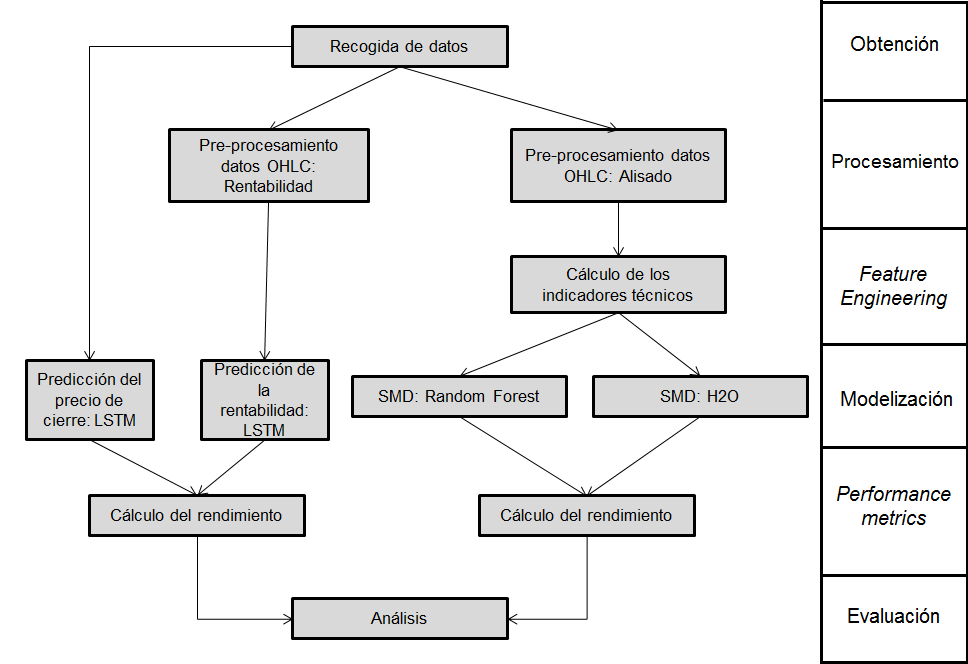
\includegraphics[width=6.51042in,height=8.33333in]{metodologia3.png}
\centering
\captionof{figure}{Metodología propuesta. Fuente: elaboración propia}

\justifying

\FloatBarrier
\newpage
\fancyhead[L]{CONSECUENCIAS DE LA IMPLANTACIÓN DE LA IA EN LOS MERCADOS FINANCIEROS}
\fancyhead[R]{\thepage}
\fancyfoot[C]{}

\chapter{\textbf{CONSECUENCIAS DE LA IMPLANTACIÓN DE LA IA EN LOS MERCADOS FINANCIEROS}}

\noindent En el presente capítulo se procede a analizar las
consecuencias de la implantación de la inteligencia artificial en los
mercados y el sector financiero. En primer lugar se analiza la
proyección histórica y la evolución de la inteligencia artificial como
campo de estudio, así como el desarrollo paralelo a lo largo de la
historia de las aplicaciones sobre el mundo de las finanzas de la misma.
Posteriormente se estudian las aplicaciones actuales de los modelos de
machine learning e IA para observar las consecuencias actuales y
discutir las posibles consecuencias futuras.

\FloatBarrier
\fancyhead[L]{Evolución histórica y contexto actual}
\fancyhead[R]{Capítulo \thechapter}
\fancyfoot[C]{\thepage}

\section{III.1 \textbf{Evolución histórica y contexto actual}}

\justifying

\noindent La Inteligencia Artificial, más conocida como AI por sus
siglas en inglés, es un campo de estudio que se ha venido desarollando
por oleadas los últimos 70 años. Sin embargo, este nuevo campo de la
ciencia tiene como fundamentos ideas y técnicas tomadas de otros campos
de estudio lárgamente establecidos. Estos otros campos son la filosofía;
tomando las ideas de razón, lógica y mente; las matemáticas, la cuál
aportó teorías sobre la lógica, deducción e inducción, probabilidad,
toma de decisiones y cálculo; la psicología, la linguística y la ciencia
computacional (Stuart Russel, 1995).

\setlength\parskip{5ex}

\textbf{Nacimiento, primera oleada expansiva y primer invierno}

\noindent El nacimiento de la inteligencia artificial se puede datar a
principios de la década de 1950, en la cual los científicos de la época
empezaron a plantearse por primera vez la posibilidad de crear máquinas
que pensaran. En este sentido, se empezaron a plantear la idea de crear
un cerebro artificial. Este primer periodo de la inteligencia artificial
culminará el año 1956 con la conferencia de Dartmouth la cual se puede
considerar el nacimiento de la IA al reunir a 11 matemáticos y
científicos en lo fué una gran lluvia de ideas alrededor del campo
(workshop, 2019).

\setlength\parskip{5ex}

\noindent En este sentido destaca, por ejemplo, la aportación que hizo
Alan Turing en la década de los 50. Turing escribió un artículo en el
cual especulaba con la posibilidad de crear máquinas que ``pensaran''.
En este sentido se dió cuenta de que ``pensar'' era un concepto difícil
de definir y por ello creó su famoso Test de Turing. Éste era una prueba
de la habilidad de una máquina de mostrar un comportamiento inteligente,
equivalente o indistiguible, del comportamiento inteligente de un
humano. La imagen siguiente ilustra el Test de Turing.

\centering

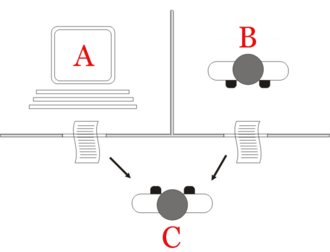
\includegraphics[width=3.125in,height=2.08333in]{Turing_test_diagram.png}
\centering
\captionof{figure}{Diagrama del Test de Turing. Fuente: Wikipedia, adaptado de "Turing Test: 50 Years Later", Saygin, 2000}

\setlength\parskip{5ex}
\justifying

\noindent El Test de Turing consiste básicamente en que el agente C, el
interrogador, tiene la tarea de intentar descubrir cuál de los dos
interrogados es una máquina, basándose sólamente en respuestas escritas
a ciertas preguntas. Si el interrogador no es capaz de distinguir cuál
de los dos agentes, A o B, es la máquina, se dice que esta máquina ha
pasado el test ya que es capaz de generar respuestas que son muy
parecidas a las respuestas que daría un humano. La idea que tenía Turing
es que si la máquina es capaz de pasar el test entonces es razonable
afirmar que la máquina estaba ``pensando'', al ser sus respuestas
indistinguibles a las que daría un humano.

\noindent La época que siguió a la conferencia de Dartmouth 1956 fue una
era de descubrimientos en el nuevo campo recién creado. Se desarrollaron
los primeros programas capaces de demostrar teoremas de geometría y
aprender los primeros idiomas como el Inglés. Sin embargo esta etapa de
desarrollo de los primeros programas de inteligencia artificial llegó a
su fin a mediados de los años 1970s. La limitada capacidad computacional
y potencia de procesamiento de las máquinas de la época dificultó que la
expansión continuara, al ser el límite material a las ideas de la época.
Pese a que las limitaciones computacionales fueron el principal
impedimento para que esta primera ola de desarrollo de la IA continuara,
otros problemas derivados como la pérdida de la financiación obtenida
durante la primera expansión o las críticas recibidas por parte de otros
científicos de distintos campos, como la filosofía, contribuyeron a la
finalización de esta primera etapa de expansión (Stuart Russel, 1995).

\textbf{Segunda oleada}

\noindent La segunda oleada la podemos ubicar en los años 1980s. Esta
etapa está definida por tener a los \textbf{sistemas expertos} como
centro gravitatorio. A principios de los años 80 este tipo de programas
de inteligencia artificial se empezaron a utilizar a nivel empresarial y
se popularizaron. Un sistema experto es un tipo de programa de
inteligencia artificial que resuelve cuestiones o problemas relacionados
con un campo de conocimiento muy específico, basándose en normas y
reglas lógicas derivadas del conocimiento de los expertos en esa
materia. Este tipo de programas intentan emular el comportamiento de
tendría un experto en un determinado campo de estudio al intentar
resolver el problema. Intentan crear, en definitiva, poder computacional
``inteligente'' que permita suplir al poder cerebral humano (Leondes,
2002). En este sentido fueron los primeros programas de inteligencia
artificial que se podían considerar útiles al tener un diseño
relativamente sencillo cuyo mantenimiento y desarrollo era relativamente
asequible. El alza de los sistemas expertos puso en el centro de la
inteligencia artificial el concepto de \textbf{conocimiento} y empezaron
a plantearse la idea de que la inteligencia podía derivarse del uso
intensivo de una gran fuente de conocimiento y la capacidad de
utilizarlo e interconectarlo de distintas maneras (Stuart Russel, 1995).

\noindent Fue llegados a este punto, con el auge de los sistemas
expertos, cuando aparecieron las primeras aplicaciones en el mundo de
las financias utilizando este tipo de sistemas computacionales. Uno de
los primeros programas que se propuso en el campo de la predicción
financiera fue el sistema experto llamado Protrader. Este sistema,
desarrollado por Ting-peng Lian y K.C Chen, fue capaz de precedir 87
puntos de caída del índice Dow Jones Industrial Average en 1986. Sus
funciones principales eran las de determinar una estrategia de inversión
óptima, ejecutar transacciones cuando eran necesarias y modificar la
base de su conocimiento mediante un mecanismo de aprendizaje. En la
figura 3.2 se puede observar un esquema de la arquitectura que tenía
este sistema experto. Más detalles pueden ser encontrados en (Chen,
1989).

\centering

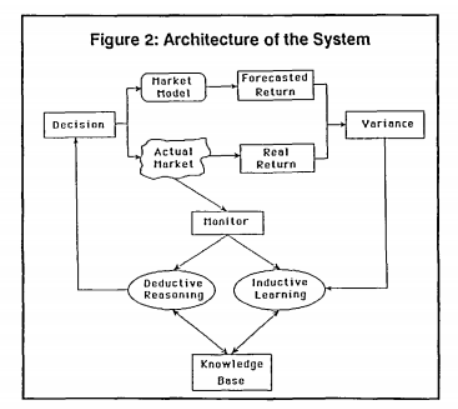
\includegraphics[width=5.20833in,height=3.64583in]{protrader.png}
\centering
\captionof{figure}{Esquema de funcionamiento de Protrader. Fuente: Chen, Liang (1989). Protrader: an Expert System for Program Trading}

\setlength\parskip{5ex}
\justifying

\noindent En esta época se desarrollaron y crearon otro tipo de
aplicaciones financieras de los sistemas expertos. Podemos encontrar
programas en el campo de la auditoría, así como en el de la
planificación financiera o los planes de inversión, ahorro y jubilación.
A su vez se empezó a explorar la posibilidad de utilizar la inteligencia
artificial en el campo de la detección del fraude, especialmente en la
decada de 1990. Uno de los programas que fue patrocinado por el
departamento del tesoro de Estados Unidos se llamaba FinCEN Artificial
Intelligence system (FAIS). Este sistema se puso en funcionamiento en el
año 1993 se podía utilizar para determinar casos de blanqueo de
capitales (Golberg, 1995). En el diagrama 3.3 se muestra la arquitectura
del FAIS. Este sistema era capaz de realizar más de 200.000
transacciones por semana, en una época en la que las transacciones eran
transcritas a mano. Por más de dos años el FAIS fue utilizado para
detectar 400 casos potenciales de blanqueo de capitales por un total de
1\$ billón (Golberg, 1995).

\centering

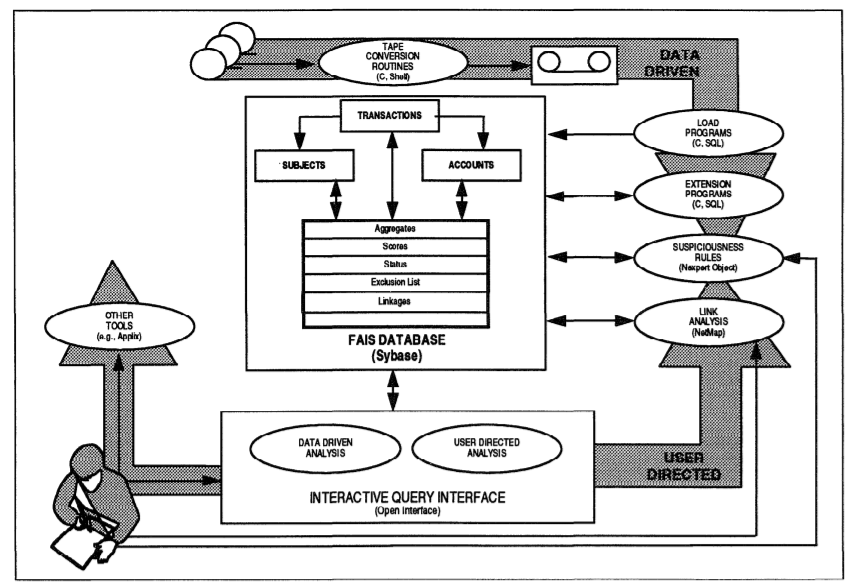
\includegraphics[width=5.98958in,height=6.77083in]{FAIS.png}

\centering
  \captionof{figure}{Esquema de funcionamiento del FAIS. Fuente: informe de la AAAI sobre FinCEN FAIS (1995)}

\setlength\parskip{5ex}
\justifying

\textbf{Tercera oleada y actualidad}

\noindent La tercera expansión de la inteligencia artificial es la que
estamos viviendo hoy en día. Empezó a principio de la década de los 90
con la unión de la inteligencia artificial con ideas económicas. La
definición de agente racional proveniente de la teoría de la decisión
casó con ideas de la ciencia computacional y apareció la definición de
agente inteligente. Los agentes inteligentes son sistemas que perciben
el entorno en el que están y toman acciones que maximizan sus
probabilidades de éxito. Son programas que vehiculan su actividad en
base a la obtención de objetivos dentro de un entorno concreto. Otro
ejemplo de los programas desarrollados a principios de los 90 es el
sistema conocido como Deep Blue, que fue el primer ordenador entrenado
para jugar al ajedrez que pudo batir al campeón mundial de ajedrez,
Garry Kasparov (McCorduck, 2004).

\noindent Estos avances a principios de la década de los 90 facilitaron
la enorme expansión de la inteligencia artificial a principio del siglo
XXI. Actualmente, la situación está dominada por el incremento en la
potencia computacional de los ordenadores, que permite procesar una
cantidad muy elavada de información de distintos tipos (Big Data), así
como la utilización de técnicas avanzadas de aprendizaje automático
aplicadas de manera exitosa en distintos campos de negocio. Es indudable
que la inteligencia artificial forma parte de nuestra vida diaria ya que
sus distintas aplicaciones se pueden apreciar de manera clara en la
sociedad de hoy en día. En general, los campos exitosos que se están
desarrollando en la actualidad son los siguientes:

\begin{enumerate}
\def\labelenumi{\roman{enumi})}
\item
  \textbf{Deep Learning}: Es un campo del machine learning que permite
  modelar altos niveles de abstracción en los datos con la construcción
  de redes neuronales más complejas. Los campos más desarrollados dentro
  del deep learning son las redes convolucionales profundas y las redes
  neuronales recurrentes (como las Long Short Term Memory). Su
  implantación en el mundo real es más que notoria ya que se utilizan de
  una manera satisfactoria, por ejemplo, en problemas de reconocimiento
  de imágenes.
\item
  \textbf{Big Data}: El término Big Data hace referencia al tipo de
  información que no puede ser capturada, tratada y procesada con los
  medios de software tradicionales, por lo que es necesario un nuevo
  paradigma para el tratamiento de este tipo de datos. A los datos Big
  Data se los suele caracterizar con 5 V's (aunque se pueden encontrar
  artículos que postulan incluso 8). Éstas son: Volúmen, Velocidad,
  Variedad, Valor y Veracidad. La V de volúmen hace referencia al tamaño
  de los datos Big Data, que suele alcanzar magnitudes superiores al
  TeraByte de capacidad. La Velocidad hace referencia a la alta
  frecuencia de generación de este tipo de datos, que junto con su
  elevado volúmen, hace necesaria una nueva manera de capturar estos
  datos de una manera frecuente y rápida. Variedad hace referencia al
  hecho de tener distintos tipos de información, todos ellos relevantes.
  Desde datos en formato tabular hasta imágenes o secuencias de texto.
  Valor hace referencia al hecho de que sean datos capaces de ayudar a
  solventar un problema y aportar valor añadido. Por último, la V de
  veracidad hace referencia al hecho de que sean datos en los que
  realmente se puedan basar ciertas conclusiones.
\end{enumerate}

\setlength\parskip{5ex}
\justifying

\noindent La figura 3.4 que se muestra a continuación permite obtener
una visión más general de la situación en la que se encuentra la
inteligencia artificial actualmente. El gran volúmen de datos
disponibles para ser tratados junto con el aumento de la capacidad
computacional han permitido tal evolución que se han desarrollado
distintas ramas dentro del mismo. El campo de la inteligencia artificial
se puede definir hoy en día como aquél dedicado a desarrollar sistemas
computacionales capaces de llevar a cabo tareas que tradicionalmente
requerían inteligencia humana para ser llevadas a cabo (Board, 2017). El
campo dentro del marco de la inteligencia artificial que más se está
desarrollado es el llamado Machine Learning o aprendizaje automático. Se
puede definir como el conjunto de métodos y algoritmos los cuales se
optimizan a través de la experiencia con intervención limitada o
inexistente de un agente humano (Board, 2017), (Jordan \& Mitchell,
2015). Estas técnicas, mezcladas con las procedentes del campo del Big
Data y el tratamiento masivo de datos, se utilizan para extraer
información de valor de conjuntos de datos muy grandes y que suelen
incorporar formatos no tabulares de información.

\centering

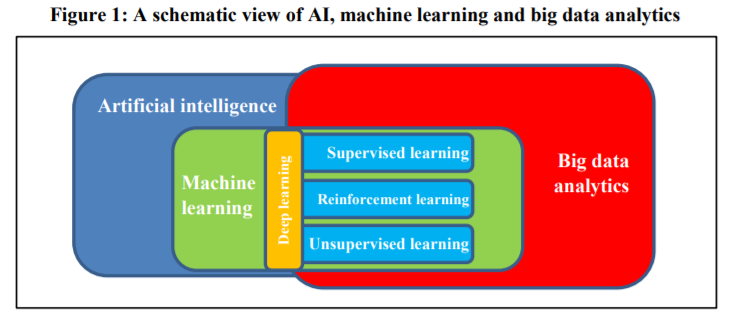
\includegraphics[width=4.6875in,height=2.60417in]{schemaAI.png}
\centering
\captionof{figure}{Esquema AI. Fuente: Artificial intelligence and machine learning in financial services. Financial Stability Board (FSB) 2017}

\setlength\parskip{5ex}
\justifying

\noindent En el mundo actual se pueden encontrar múltiples aplicaciones
de inteligencia artificial y modelos de machine learning. En este
sentido las empresas llamadas ``fintech'' ya se encuentran totalmente
implantadas en la sociedad actual. Esto es así debido a que son empresas
que prestan servicios financieros de una manera más dinámica que el
sector bancario o financiero tradicional, apoyándose en las nuevas
tecnologías y paradigmas de los sistemas de información de la
actualidad. Así mismo, estas empresas están ejerciendo un efecto
dinamizador en cuanto al desarrollo y digitalización de los sectores
bancarios y financieros más tradicionales. España contaba a finales de
2017 con 300 Fintech y ocupaba la sexta posición en el mundo por número
de compañías en el sector. Un informe elaborado por KPMG confirma que el
modelo de negocio mayoritario de las Fintech nacionales es el de
préstamos (21\%), seguido del sector de pagos (19\%) y el de inversión
(16\%) (Funcas, 2017).

\FloatBarrier
\fancyhead[L]{Aplicaciones y consecuencias}
\fancyhead[R]{Capítulo \thechapter}
\fancyfoot[C]{\thepage}

\section{III.2 \textbf{Aplicaciones y consecuencias}}

\noindent En un mundo donde los datos juegan un papel fundamental (hay
quién incluso los llama el petróleo del siglo XXI) y el tratamiento de
la información está totalmente implantado, todos los ámbitos de la
realidad se ven afectados. En el caso del mundo de las finanzas el
impacto ha sido profundo. En los últimos años el campo de la
inteligencia artificial ha sido capaz de crear sistemas computacionales
y aplicaciones en el campo de las finanzas. En la sección siguiente se
examinan los distintos campos del sector financiero en los cuales se
aplican actualmente técnicas de machine learning e inteligencia
artificial con el objetivo de poder examinar con detalle las
consecuencias actuales de su implantación así como las posibles
implicaciones futuras. Éstos son: (3.2.1) centrados en el cliente (o
\emph{front office}), que incluyen el \emph{credit scoring},
aplicaciones en el campo de los seguros de vida y no vida, y los
chat-bots encargados de interactuar con el cliente; (3.2.2) centrados en
las operaciones (o \emph{back office}), con casos como los modelos de
gestión del riesgo y modelos de impacto de mercado; (3.2.3) gestión de
carteras y inversión en mercados financieros; (3.2.4) casos en los que
instituciones financieras y empresas privadas aplican la IA y el
aprendizaje automático en regulación y supervisión; y (3.2.5) otras
aplicaciones.

\justifying

\FloatBarrier
\fancyhead[L]{Aplicaciones front office: centradas en el cliente}
\fancyhead[R]{Capítulo \thechapter}
\fancyfoot[C]{\thepage}

\subsection{III.2.1 \textbf{Aplicaciones front office: centradas en el cliente}}

\justifying

\textbf{Credit scoring}

\noindent La evaluación del crédito ha sido un método lárgamente usado
por los prestamistas a la hora de prestar o no un crédito. La capacidad
de evalúar el potencial riesgo del préstamo, otorgándole un valor, de un
determinado cliente es esencial para las compañías financieras. La
aplicación de técnicas de aprendizaje automático en este sector se está
estableciendo lárgamente entre las distintas instituciones encargadas de
prestar dinero. Tradicionalmente se han utilizado datos estructurados
como transacciones y el historial de pagos para crear modelos tales como
regresiones lineales o árboles de decisión para generar un ránking o
valoración de crédito. Sin embargo en la actualidad los prestamistas, ya
sean bancos o otras comañías, están utilizando ya otras fuentes de datos
no estructurados o semi estructurados tales como la actividad en las
redes sociales, uso del teléfono móvil o mensajes de texto. Este tipo de
datos permite a estas empresas obtener una visión más matizada de la
fiabilidad potencial que tendría un préstamo. La aplicación de modelos
de IA y ML sobre esta gran variedad de tipos de datos ha permitido a las
empresas prestamistas analizar factores cualitativos como el
comportamiento del consumo de los clientes o la valoración de la
voluntad de pagar el préstamo.

\setlength\parskip{5ex}

\noindent Una de las principales consecuencias de la capacidad de
manejar distintas fuentes de información ha sido el hecho de que
actualmente es que la segmentación de la calidad de los prestatarios se
hace a mayor escala, de una manera más rápida y más barata. En
definitiva esto radica en una \emph{decisión de crédito más rápida y
acurada} (Stefan Lessmann \& Thomas, 2015). Otra de las consecuencias de
la aplicación del machine learning en este sector es el hecho de que
puede ayudar a garantizar un mayor acceso al crédito. Esto es así ya que
los sistemas de evaluación de crédito tradicionales necesitan una
cantidad suficiente de datos históricos sobre crédito de esa persona
para poder considerarla apta para la evaluación. Si esta información no
está disponible, el valor de la evaluación del crédito no puede ser
generado y el cliente puede ser potencialmente incapaz de obtener un
crédito. Con el uso de fuentes de datos alternativas y la aplicación de
modelos de aprendizaje automático los prestamistas son capaces de llevar
a decisiones de crédito que hubieran sido imposibles anteriormente
(Board, 2017).

\setlength\parskip{5ex}

\noindent En general se pueden observar ventajas e inconvenientes de
utilizar inteligencia artificial o machine learning en el sector de la
evaluación del credito. Como ventaja se encuentra el hecho de que la IA
permite analizar una cantidad enorme de datos de una manera rápida. Esto
implica que el coste de evaluar los riesgos de los potenciales clientes
se verá reducido. Además, el hecho de introducir nuevos tipos de datos
puede permitir a las compañías el evaluar el riesgo de crédito de
individuos para los cuales no se podía evaluar utilizando los datos
tradicionales (historial de crédito). Es decir, la falta de historial de
crédito o una valoración anterior de crédito ya no serán más un
impedimento a la obtención de un crédito ya que otros indicadores de la
verosimilitud del pago están siendo utilizados por las compañías.

\setlength\parskip{5ex}

\noindent Sin embargo, el uso de complejos algoritmos de machine
learning puede conducir a una falta de transparencia con el consumidor.
Cuando se utilizan modelos de machine learning para construir una
valoración o puntuación de crédito, es generalmente más difícil el poder
ofrecer una explicación sobre esa valoración y la posterior decisión a
los clientes, auditores y supervisores. La faceta \emph{black box} que
tienen normalmente estos algoritmos lo complica. Además, ciertos autores
argumentan que la utilización de fuentes de datos alternaticvas, tales
como comportamiento online o fuentes de información financiera no
tradicionales, puede introducir \textbf{sesgo} en las decisiones de
crédito (O'Neil, 2016). En este sentido ciertas asociaciones de
consumidores han levantado la voz en cuanto al aspecto moral. Los
modelos de machine learning pueden llevar perfiles de prestatario que
tengan en consideración la raza o el género. Por ejemplo, estos modelos
pueden puntuar a un prestatario de una minoría étnica con un mayor
riesgo por defecto sólo porque prestatarios similares han tenido
tradicionalmente unas condiciones menos favorables de crédito.

\setlength\parskip{5ex}

\textbf{Servicios de seguros}

\noindent El sector de los seguros es uno de los sectores que más confía
en el análisis de datos y la inteligencia artificial para llevar a cabo
su negocio. De hecho, el análisi estadístico representa el núcleo
fundamental de este tipo de negocio. La capacidad de evalúar el precio
de un producto asegurador es esencial para este sector para poder ser
rentable. Todas estas técnicas se basan en un análisis masivo de grandes
bases de datos que las empresas aseguradoras han venido recolectando
desde hace años para evaluar el riesgo de un potencial cliente. De esta
manera consiguen ofrecer servicios más baratos a aquellas personas con
un menor riesgo potencial o inrcementarlo para aquellas personas con más
riesgo. Un claro ejemplo que el lector es posible que haya experimentado
es el hecho de ver como incrementa la cuota de su seguro de automóvil
después de tener un accidente de tráfico.

\setlength\parskip{6ex}

\noindent Sin embargo, muchas de las aplicaciones actuales de técnicas
de machine learning incorporan el análisis de datos desestructurados
para mejorar el proceso de suscripción de los seguros, apoyando la
asignación de un precio en función de las características del potencial
cliente, o para fortalecer estrategias de márketing hacia determinados
clientes (segmentación). Ejemplos de estos nuevos tipos de datos son los
datos en tiempo real y los datos con alta granularidad. Ejemplos de
estos últimos son datos relacionados con el comportamiento de compra
online o datos telemétricos provinientes de sensores en aparatos
electrónicos. En este sentido, estas empresas empiezan a explorar cómo
pueden aplicar la IA y el machine learning sobre datos de sensores
remotos, conectados a través del \emph{Internet of Things (IoT)}, para
detectar e intentar prevenir accidentes susceptibles de ser asegurados
(como accidentes de coche).

\setlength\parskip{5ex}

\textbf{Chat Bots}

\noindent Otra de las aplicaciones actuales de la inteligencia
artificial en el campo del \emph{front end} son los llamados ChatBots
que se encargan de interactuar con el cliente. Los Chat Bots son
programas automáticos que se encargan de asistir y/o ayudar a los
clientes en sus transacciones diarias o para resolver problemas. Estos
programas utilizan una rama del machine learning llamada NLP
(procesamiento del lenguaje natural) para interactuar con los clientes
en lenguajes naturales, ya sea por texto o por voz. Este tipo de
programas están siendo introducidos por numerosas compañías de servicios
financieros, especialmente en sus aplicaciones móviles o las redes
sociales, con el fin de agilizar la relación con el cliente y captar
nuevas generaciones de clientes.

\noindent Actualmente los algortimos Chat Bot que se están utilizando
son relativamente sencillos y se centran en informar al cliente y
resolver cuestiones sencillas. Sin embargo, los Chat Bots se están
moviendo cada vez más hacia las recomendaciones, especialmente en las
decisiones financieras importantes. Además, este tipo de modelos
permiten a las compañías obtener información de sus clientes gracias a
la interacción con estos programas. Ejemplos de sectores que utilizan
actualmente los Chat Bots en el mundo financiero son las instituciones
financieras y las compañías de seguros. Éstas utilizan los Chat Bots
para dar consejos sobre seguros en tiempo real.

\noindent Una de las principales consecuencias de la implantación de los
Chat bots en el \emph{front office} del sector financiero es algo muy
obvio pero a la vez muy importante. Este tipo de programas consiguen
reducir las relaciones humanas en el sector financiero. Es posible que
en un futuro un gran porcentage de las interacciones entre los clientes
y el sector financiero se hagan a través de este tipo de programas, o de
otros más complejos que se puedan desarrollar en el futuro.

\setlength\parskip{5ex}

\FloatBarrier
\newpage
\fancyhead[L]{Aplicaciones back office: centradas en las operaciones}
\fancyhead[R]{Capítulo \thechapter}
\fancyfoot[C]{\thepage}

\subsection{III.2.2 \textbf{Aplicaciones back office: centradas en las operaciones}}

\justifying

\textbf{Modelos de gestión de riesgo: validación y stress-tests}

\noindent El llamado back-testing, o validación de modelos de gestión de
riesgo, es importante para el secto bancario porque ha sido utilizado
tradicionalmente para evaluar si los modelos de riesgo de los bancos
funcionan bien o no. Este tipo de modelos agrupa por ejemplo modelos de
gestión de riesgo de crédito, de liquidez, de mercado (tipo de cambio,
tipo de interés, cotización\ldots{}) o riesgo operacional. La validación
de modelos se define como el conjunto de procesos y actividades que
tienen como objetivo el verificar que los modelos, en este caso de
riesgo, están rindiendo como se esperaba, en línea con los objetivos por
los cuales se diseñaron y para evaluar su posible impacto (Mitchell,
2016). En este sentido, los bancos están empezando a considerar el
machine learning para poder utilizar y hacer que tenga sentido grandes
bases de datos estructurados y no estructurados y para analizar el
output de los modelos primarios. El hecho de utilizar este gran conjunto
de herramientas financieras para realizar el back-testing o validación
de modelos permite considerar cambios en el comportamiento de los
mercados y otras tendencias, con el objetivo bienintencionado de reducir
la potencial infravaloración del riesgo en distintos escenarios
financieros (Mitchell, 2016).

\setlength\parskip{5ex}

\noindent Existen algunos ejemplos actuales de bancos que utilizan
modelos de aprendizaje automático no supervisados en sus validaciones de
modelos. Este tipo de modelos ayudan a los agentes validadores en el
monitoreo constante de los test de stress llevados a cabo internamente y
de una manera regulatoria, al ser éstos una ayuda para determinar si los
modelos de riesgo están rindiendo dentro de los límites aceptables o si
se están desviando de su objetivo principal. Además, pueden ofrecer
características o variables extra para los modelos de riesgo
operacional, tales como la vulnerabilidad de las distintas
organizaciones a los ciber ataques (Board, 2017).

\setlength\parskip{7ex}

\noindent A su vez, se está empezando a utilizar la inteligencia
artificial y técnicas de machine learning en el campo de los test de
estrés bancarios. Estas pruebas de resistencia bancaria consisten en
técnicas de simulación que tienen como objeivo determinar la capacidad
de estabilidad de una entidad bancaria. Consisten en exponer tanto las
carteras de activos como las de pasivos a diferentes situaciones para
evaluar las posibles reacciones o consecuencias. Este tipo de pruebas se
ha venido utilizando cada vez más después de la crisis financiera global
del año 2008. En este caso se utilizan modelos no supervisados de
aprendizaje automático para revisar grandes volúmenes de datos con el
objetivo de analizar cualquier sesgo en la selección de variables de
estos modelos de estrés. La consecuencia directa de la aplicación de la
IA en este tipo de pruebas es que conducen inevitablemente a mejores
modelos con mayor transparencia.

\setlength\parskip{5ex}

\textbf{Modelización del impacto de mercado}

\noindent El análisis de impacto de mercado consiste en evaluar el
efecto que tiene sobre los precios de mercado las acciones de
compra/venta (\emph{trading}) que hace una empresa. Para las compañías
de \emph{trading} es importante el poder evaluar el impacto que tienen
sobre los precios de mercado las operaciones que ejecutan, en especial
aquellas operaciones de gran volúmen. En este sentido es esencial para
ellas tener una estimación más precisa del impacto que tienen las
operaciones que ejecutan de manera que se pueda ajustar la periodicidad
de las mismas y minimizar los costes de ejecución de las operaciones.
Las compañías financieras están utilizando ya la IA para obtener más
información de los modelos que han utilizado históricamente, haciéndolos
más fuertes y potentes, así como para ayudar a identificar relaciones no
lineales entre las ordenes de compra y venta. Los modelos de machine
leaning que se están creando, llamados \emph{trading robots}, se
entrenan a ellos mismos para saber cómo reaccionar a los cambios en el
mercado (Day, 2017).

\setlength\parskip{5ex}

\noindent Algunos de los ejemplos concretos de herramientas que utilizan
el machine learning para modelizar el impacto de mercado son los
siguientes. Actualmente se utiliza la IA para identificar grupos de
bonos que se comportan de manera similar. De esta manera, las compañías
pueden agrupar distintos bonos o activos financieros en grupos
utilizando técnicas de \emph{cluster} con el objetivo de poder medir y
valorar la liquidez de los bonos de manera individual. Otro de los
ejemplos de aplicación de la IA en este campo es el uso que se hace de
ella para identificar cómo la sincronización de las operaciones puede
minimizar el impacto de mercado. Estos modelos intentar evitar el hecho
de programar operaciones muy cercanas en el tiempo con el objetivo de
esquivar tener un impacto de mercado mayor que la suma de los impactos
individuales. Estos modelos se utilizan para decidir la mejor
programación de las operaciones (temporalmente hablando) y para
modificar esta programación temporal a medida que la compra venta se va
produciendo a tiempo real. Para modelizar estos cambios de utilizan
técnincas de aprendizaje automático supervisado.

\FloatBarrier
\fancyhead[L]{Gestión de carteras e inversión en mercados financieros}
\fancyhead[R]{Capítulo \thechapter}
\fancyfoot[C]{\thepage}

\subsection{III.2.3 \textbf{Gestión de carteras e inversión en mercados financieros}}

\justifying

\textbf{Inversión y trading algorítmico}

\noindent Otro de los campos en los que se aplica actualmente la IA es
en el del \emph{trading algorítmico}. Estos sistemas de machine learning
son entrenados con información de grandes bases de datos relacionadas
con las condiciones cambiantes del mercado en cuestión y el precio para
extraer una decisión de inversión, compra o venta de una posición, y
colocarla en el mercado. Aquí entra en juego de nuevo el gran potencial
del big data y el machine learning a la hora de procesar un gran volúmen
de información de una manera muy rápida, potencialmente en tiempo real.
Estos algoritmos están constantemente analizando el mercado y posteando
acciones de compra o venta de una posición con una frecuencia muy
elevada. Es a causa de la gran velocidad en las interacciones con el
mercado generada con este tipo de sistemas que se los mercados
tradicionales se están adaptando al llamado \emph{High-Frequency Trading
(HFT)}. El \emph{trading} de alta frecuencia se soporta sobre este tipo
de algoritmos de \emph{trading} automático, que permiten alcanzar
niveles donde el ser humano no sería nunca capaz de llegar ya que no
podemos procesar tal cantidad de información de una manera tan rápida.

\setlength\parskip{5ex}

\noindent Las consecuencias de la implantación de las transacciones
bursátiles de alta fracuencia han sido tanto positivas y negativas. En
primer lugar una de las principales consecuencias positivas de la
aplicación del \emph{trading} algorítmico y la creación del llamado HFT
ya ha sido nombrada. Es el hecho de que las transacciones aumentan de
velocidad. Al ser transacciones automatizadas que se hacen de una manera
rápida en cuanto hay un cambio favorable en el mercado, también aumenta
en consecuencia el número de transacciones totales que se realizan en
ese mercado, a la par que disminuyen el número de transacciones con un
mayor volúmen. En otras palabras, transacciones de menor volúmen y más
rápidas. Otra de las consecuencias generales que se pueden apreciar es
que el hecho de introducir HFT, y la algorítmica en general, en los
mercados financieros de \emph{trading} es que se ha reducido el coste de
las transacciones. La razón es sencilla: es más asequible hacer
\emph{trading} o negociación bursátil con máquinas que con humanos, ya
que las primeras tienes ciertos beneficios tales como no requerir días
de vacaciones o no ponerse enfermos (entre otros). Es por eso que el
coste el coste de las transacciones se ha venido reduciendo a medida que
los mercados se han ido automatizando. El hecho de poder sustituir
factor de trabajo humano por factor capital, al reproducir las tareas
que anteriormente hacían los \emph{brokers} o \emph{traders}, tiene como
consecuencia directa una reducción del coste de las transacciones. En
tercer lugar, existen estudios que demuestran que la diferencia entre el
precio de compra/oferta y de venta/demanda en un mercado financiero,
también conocido como \emph{bid-ask spread}, se ha reducido a causa de
la implantación del HFT. Por consecuencia la liquidez, definida como el
valor disponible para comprar y vender dentro del rango de precios
Bid-Ask, se ha incrementado a lo largo del tiempo (Oliver Linton, 2018,
p. 13). Otra de las consecuencias positivas del HFT se puede encontrar
en términos de estabilidad y predictibilidad de los mercados. Hay una
gran evidencia que sugiere que la eficiencia del precio, en los mercados
financieros, se ha incrementado generalmente con el crecimiento de las
operaciones bursátiles basadas en computación (Oliver Linton, 2018). Se
ha comprovado que los traders de HFT tienden a mover las operaciones en
la dirección de los cambios de precios permanentes (eficientes, óptimos)
y en la dirección opuesta a los precios transitorios erráticos (Jonathan
Brogaard \& Riordan, 2013).

\setlength\parskip{5ex}

\noindent Es totalmente cierto que, por otro lado, el hecho de
incorporar las transacciones bursátiles de alta frecuencia en los
mercados financieros ha traído, y puede provocar en el futuro, ciertas
consecuencias no tan deseables. Uno de los principales argumentos que se
esgrime en numerosos estudios en contra del HFT es que éste aumenta la
volatilidad de los mercados, aludiendo al hecho de que la volatilidad es
más elevada en mercados más rápidos. Además, al ser un sistema nuevo, es
posible que este tipo de algoritmos, que unitariamente pueden ser
estables, terminen funcionando de una manera inconsistente o muy
inestable. Sin embargo, existen toda otra serie de estudios, analizados
en detalle en (Board, 2017) p.16, que ponen en evidencia una falta de
eventos empíricos que soporten esta teoría. En general los datos no
confirman el hecho de que el HFT haga que los mercados sean más
volátiles. Otra de las consecuencias negativas que podrían tener graves
implicaciones, especialmente en el futuro, es la que se puso de
manifiesto el día 6 de Mayo de 2010 en el índice E-mini S\&P 500 del
mercado de futuros en EEUU. En esta fecha se produjo lo que se llamó un
\emph{Flash-Crash}, es decir, un evento intra-día de corta duración en
la que se produce un desajuste profundo de los precios que no está
generado por ningún cambio en el valor fundamental de los activos que se
están comprando/vendiendo. En el caso del \emph{Flash-Crash} del 2010,
se ejecutranon en un corto plazo de tiempo muchos algoritmos de HFT con
órdenes de venta, motivo por el cual el precio presentó una gran
volatilidad durante unos minutos. La figura 3.5 muestra la trayectoria
del precio de los futuros en este mercado durante el crash, así como los
cambios en los precios entre transacciones consecutivas, medidos en
ticks. Gracias a ella podemos observar la gran velocidad con la que
cambió el precio y la increíble volatilidad durante este periodo.

\centering

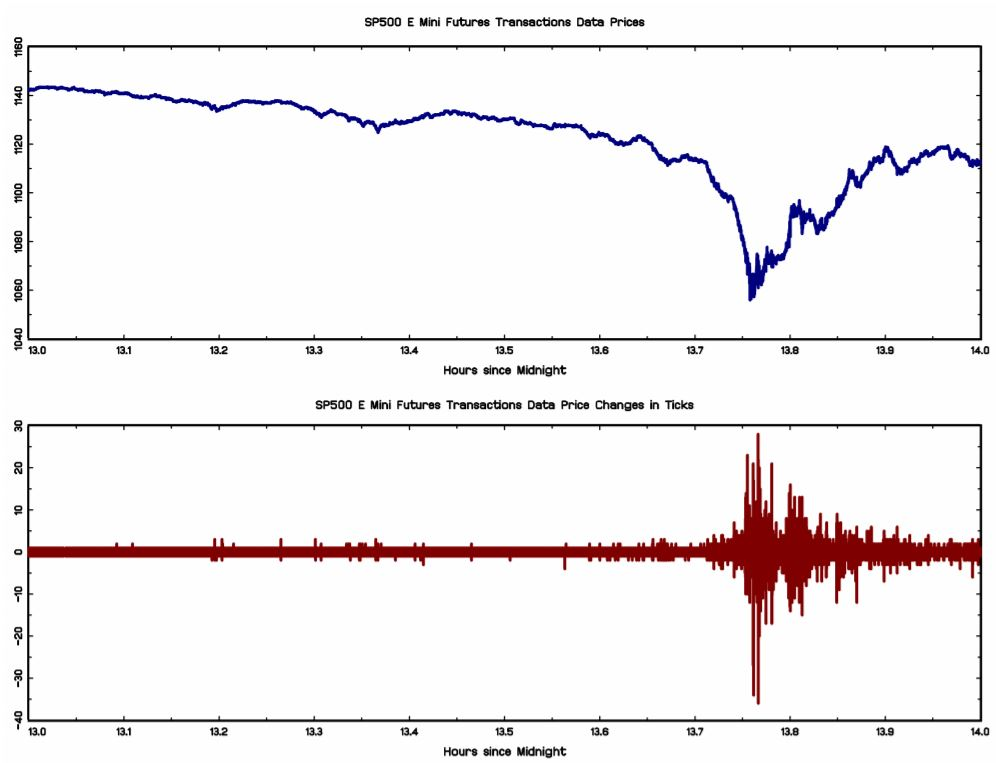
\includegraphics[width=7.8125in,height=5.20833in]{flashcrash1.JPG}
\centering
\captionof{figure}{Nivel de precios de los futuros Emini durante el flash crash y cambios en los precios entre transacciones consecutivas. Fuente: Implications of high-frequency trading for security markets, Oliver Linton, Soheil Mahmoodzadeh 2018}

\justifying
\setlength\parskip{5ex}

\noindent Una de las posibles causas de este \emph{Flash-Crash} se
encuentra detalladamente descrita en (Oliver Linton, 2018). En un
informe de la SEC/CFTC (2010) se propone como punto inicial una gran
orden de venta de 75000 contratos de futuros. Esto provocó que los
algoritmos de trading automático empezaran a interactuar entre ellos
tratando de absorver el gran volúmen. En general, este informe concluye
que los traders de alta frecuencia no fueron los que desencadenaron el
\emph{Flash-Crash} pero fueron sus respuestas a la presión de venta
inusual generada ese día, ejecutadas a gran velocidad, las que
provocaron que la volatilidad del mercado se viera amplificada.

\setlength\parskip{5ex}

\noindent Existen otros ejemplos de \emph{Flash-Crashes} entre los que
cabe destacar la comúnmente llamada ``Pesadilla en Wall-Street'' el 1 de
Agosto de 2012. En este caso, la compañia Knight Capital perdió
alrededor de 450 millones de dólares en unos pocos minutos a causa de un
``error de \emph{trading}'' que provocó un un desajuste transversal en
el NYSE. Otros ejemplos los podemos encontrar en los mercados de
divisas. Es el caso del llamado \emph{Sterling Flash Crash} ocurrido en
2016, donde el par GBP/USD, el tercero más líquido en el mundo,
disminuyó el valor un 9.66\% en 40 segundos (Oliver Linton, 2018).

\setlength\parskip{5ex}

\noindent En general, las transacciones bursátiles de alta frecuencia
pueden mejorar la calidad de los mercados, generando mayor liquidez,
reduciendo los márgenes entre precios de oferta y demanda (\emph{bid-ask
spread}) y aumentando la eficiencia. No obstante los beneficios que el
HFT aporta pueden venir con una serie de costes asociados, como ya se ha
destacado. La capacidad de estos sistemas automáticos de interactuar
entre ellos de una manera autónoma incrementa el riesgo de que se
produzcan eventos extremos que, aun siendo raros y excepcionales, se
inician y desarrollan a velocidades muy elevadas. Estas situaciones
generan grandes volúmenes de información que requieren largos periodos
de tiempo para ser analizados antes de ser entendidos.

\setlength\parskip{5ex}

\textbf{Gestión de carteras}

\noindent El uso de la inteligencia artificial y el machine learning en
el sector de la gestión de carteras es considerablemente importante.
Estas técnicas se utilizan para sacar provecho de la gran cantidad de
datos disponibles en los mercados para identificar nuevas señales en los
movimientos de los precios. Sin embargo, estas técnincas se fundamentan
en los mismos principios que las técnincas analíticas que ya se
utilizaban tradicionalmente. La idea es indentificar señales que
permitan hacer predicciones relacionadas con los precios o la
volatilidad de los \emph{stocks} para generar rentabilidades más grandes
y no correlacionadas. Especialmente se encuentra una gran implantación
en los fondos \emph{quant}, la mayoría de los cuales son fondos de
cobertura. A su vez se pueden encontrar también ejemplos de compañías
que utilizan técnicas de machine learning para recomendar a sus clientes
estrategias de inversión personalizadas y automatizadas, de manera que
se consigue un servicio personalizado ajustado a las necesidades
específicas de cada cliente.

\FloatBarrier
\fancyhead[L]{Regulación y supervisión}
\fancyhead[R]{Capítulo \thechapter}
\fancyfoot[C]{\thepage}

\subsection{III.2.4 \textbf{Regulación y supervisión}}

\justifying

\textbf{Detección de fraude}

\noindent Otra de las aplicaciones actuales es en el campo de la
detección de fraudes o anomaías. Los modelos y técnicas de inteligencia
artificial ayudan a identificar conductas o comportamientos que se
alejan de los patrones regulares. Estos modelos se utilizan por ejemplo
para detectar patrones complejos y para hacer hincapié en las
transacciones sospechosas que son potencialmente más serias y peligrosas
y que por lo tanto requieren una mayor atención y cuidado. Utilizando
estas técnicas junto con distintos métodos de machine learning para
analizar datos de una manera más desagregada de transacciones, perfiles
de clientes y distintos tipos de datos desestructurados, el mundo de la
inteligencia artificial se está utilizando para descubrir relaciones no
lineales entre los diferentes atributos o características (variables), y
para detectar patrones complejos que reflejen potencialmente un blanqueo
de capitales (Board, 2017). En este sentido ayuda a agilizar el trabajo
de los agentes institucionales encargados de velar por la seguridad
financiera. Estos modelos están entrenados con una información que se
genera a tiempo real y su utilidad real está en ser capaces de detectar
y bloquear una transacción potencialmente sospechosa de fraude para su
posterior revisión. Este tipo de sistemas ha permitido ahorrar a las
autoridades y empresas un gran volúmen de masa monetaria.

\setlength\parskip{5ex}

\noindent En la actualidad existen numerosos ejemplos de empresas
aplicando tecnologías de machine learning. Casos como los de
deepsense.ai o feedzai.com son bastante habituales a día de hoy. Estas
empresas se dedican a ofrecer soluciones en relación a la detección del
fraude a otras empresas. En este modelo B2B (empresa-empresa) permite a
los clientes obtener soluciones personalizadas basadas en modelos y
técnicas de análisis de datos e inteligencia artificial para poderlos
utilizar en su día a día. También existen otros casos de empresas
multinacionales que ya han incorporado este tipo de técnicas. Es el caso
de Mastercard que lanzó en 2016 su nuevo sistema llamado ``Decision
Intelligence''. Este sistema intenta resolver la problemática de los
falsos positivos de fraude en transacciones genuinas, es decir,
verdaderas, utilizando algoritmos y técnicas de machine learning.

\textbf{Compromiso regulatorio}

\noindent Otra de las aplicaciones actuales de la inteligencia
artificial y el machine learning se puede encontrar en el campo de la
regulación financiera donde las instituciones financieras las están
aplicando para hacer más potente el compromiso regulatorio. Un ejemplo
de las técnicas que éstas utilizan son el procesamiento del lenguaje
natural (NLP) para monitorear el comportamiento y la comunicación de los
\emph{traders}, con el objetivo de mantener la transparencia y la buena
conducta en los mercados. Este tipo de modelos se basan en datos tales
como emails, palabra hablada, mensajes intantáneos, documentos y otro
tipo de metadatos. A su vez, también se están utilizando los modelos de
procesamiento del lenguaje natural para interpretar, y hacer más
comprensibles, regulaciones financieras como el MiFID II. Con esto se
consigue el poder automatizar reglas de control basadas en este tipo de
regulaciones.

\FloatBarrier
\fancyhead[L]{Otras aplicaciones}
\fancyhead[R]{Capítulo \thechapter}
\fancyfoot[C]{\thepage}

\subsection{III.2.5 \textbf{Otras aplicaciones}}

\justifying

\textbf{Text mining y análisis de sentimiento}

\noindent Otra de las grandes aplicaciones de la inteligencia artificial
en general, y en especial en los sectores financieros, es la creación de
modelos de procesamiento del lenguaje natural (NLP). Las compañías
financieras y empresas FinTech ofrecen servicios basados en sistemas que
incluyen el procesamiento de todo tipo de noticias, textos en redes
sociales (social media) y arículos. La creción de regresores a partir de
información escrita potencia la capacidad predictiva de los modelos,
haciendo que sea aplicado hoy en día por numerosas empresas de servicios
de inversión. No son extraño casos como las compañías AlphaSense, Kensho
o Serimag, que ofrece servicios tales como verificación de documentos de
identificación on-line o la detección de cláusulas abusivas en las
escritura o contrato de una hipoteca
(\url{https://serimag.com/en/case-studies/}). Este tipo de modelos
consigue procesar una cantidad muy elevada de información, y como se
trata de leer documentos escritos, sobrepasan enormemente la capacidad
de lectura del ser humano. Es por eso que su aplicación sigue creciendo
dentro del sector financiero y se desarrolla en nuevas herramientas o
sistemas que utilizan esta técnica.

\noindent Otra de las aplicaciones del NLP es el análisis de
sentimiento. Este conjunto de técnicas se puede considerar un subtipo de
análisis dentro del gran campo de estudio dentro del procesamiento del
lenguaje natural. Se utiliza para añadir a los modelos predictivos el
punto de sentimiento que se deriva de los textos, en general datos de
redes sociales y noticias. De esta manera se pueden construir modelos
que procesen datos a tiempo real que se pueden utilizar como proxy del
estado de animo o sentimiento de ciertos actores económicos,
utilizándolos para la predicción, por ejemplo, de la dirección de los
mercados o para definir estrategias de inversión.

\FloatBarrier
\fancyhead[L]{Análisis económico: posibles efectos}
\fancyhead[R]{Capítulo \thechapter}
\fancyfoot[C]{\thepage}

\section{III.3 \textbf{Análisis económico: posibles efectos}}

\noindent Una vez analizadas las diferentes aplicaciones actuales de la
inteligencia artificial en el sector de las finanzas, y sus
consecuencias más directas, se procede a elaborar un análisis de las
posibles efectos o implicaciones de su implantación desde una
perspectiva económica. Concretamente se distribuye el análisis en dos
partes: por un lado desde una perspectiva micro económica (o micro
financiera) y, por otro, desde una perspectiva macro económica.

\FloatBarrier
\fancyhead[L]{Análisis micro-económico}
\fancyhead[R]{Capítulo \thechapter}
\fancyfoot[C]{\thepage}

\subsection{III.3.1 \textbf{Análisis micro-económico}}

\justifying

\noindent En primer lugar se analizan los posibles efectos de la
inteligencia artificial en los mercados financieros. Una de los
conocimientos globales que se tiene actualmente es el hecho de que la IA
y el machine learning tienen el potencial para mejorar substancialmente
la eficiencia en el procesamiento de información. Eso deriva
intevitablemente en una reducción de las asimetrías en la información
que tienen los agentes económicos y por lo tanto puede reforzar la
función de información del sistema financiero. Los mecanismos por los
cuales este refuerzo podría ocurrir incluyen los siguientes factores.
Por un lado, estos sistemas de IA puede permitir que ciertos agentes en
el mercado recojan y analicen datos a mayor escala. Con este análisis
los participantes del mercado son potencialmente capaces de entender
(mejor) la relación entre distintos factores y la formulación de los
precios de mercado. Ejemplos de los distintos factores que se pueden
relacionar con el proceso de definición de los precios de mercado son
los sentimientos o estádos de ánimo extraídos de las redes sociales o
las notícias gracias a técnicas de \emph{sentiment analysis}. Esto
podría reducir las asimetrías en la información y de esta manera
contribuir a la eficiencia y estabilidad de los mercados (véase
(Securities Commissions, 2017) p.~28). Por otro lado los modelos de
machine learning e IA pueden beneficiar a los participantes en un
mercado al reducir los costes asociados a su participación. Además la IA
pude permitir a los agentes ajustar sus estrategias de inversión de una
manera casi inmediata (o en tiempo real), como respuesta a una realidad
cambiante. De esta manera se reducen en general los costes de las
transacciones en el sistema a la par que se mejora el descubrimiento de
los precios (Board, 2017). Paralelamente se observan otras
posibilidades. Si los participantes en los mercados terminan pot
utilizar técnicas similares de machine learning los riesgos
correlacionados podrían derivar en riesgos de estabilidad de los
mercados. Es decir, si el uso de \emph{traders} basados en modelos de
aprendizaje automático se empieza a ser mejor, de una manera masiva, que
el \emph{trading} clásico, esto puede provocar que muchos agentes en el
futuro decidan también utilizar este tipo de técnicas y esdevengan, en
definitiva, un sistema que puede amplificar los \emph{shocks}
financieros, tanto positivos como negativos.

\noindent En segundo lugar se analizar los posibles efectos de la IA en
las instituciones financieras. Por un lado los sistemas de machine
learning pueden mejorar los ingresos y reducir los costes para las
mismas, ya que pueden mejorar el procesamiento de distintas operaciones
que este tipo de insituciones utilizan. Al tener éstos un gran
componente computacional, el hecho de incorporar el machine learning
para automatizar y mejorar procesos de negocio rutinarios puede
trasladarse en unos costes operacionales más bajos y, en general, hacen
que estas empresas sean más rentables. Por otro lado, y como ya se ha
analizado en la presente tesis, la IA y el machine learning se pueden
utilizar y se utilizan para la gestión del riesgo. Por ejemplo, técnicas
y modelos de gestión de riesgos de cola (distribuciones de riesgos con
las colas pesadas no normales). Además también se pueden utilizar para
detectar el fraude bancario o financiero, las transacciones sospechosas
y estimando el riesgo de ciber ataques mejorando, en definitiva, el
proceso de gestión del riesgo. Sin embargo todas estas herramientas
tienen un peligro potencial ya que pueden pasar por alto nuevas fuentes
de riesgo al no estar presentes en los datos históricos utilizados para
entrenar los modelos. Otro de los posibles efectos sobre las
instituciones financieras se analiza seguidamente. El hecho de que el
desarrollo en el campo de la inteligencia artificial sea de carácter
\emph{open source} y con un uso intensivo de datos puede animar a las
instituciones financieras a colaborar con otras e incluso con otros
sectores como el comercio on-line y las economías colaborativas. En este
sentido fomenta incrementar y potencial la colaboración inter-sectorial.

\noindent En general, en el caso de las instituciones financieras
reguladoras, la aplicación de la IA puede beneficiar al sector en
general ayudando a mejorar los sistemas actuales de control, gestión y
regulación. No obstante todos estos efectos positivos vienen con unos
riesgos potenciales asociados. La creación de modelos de toma de
decisiones automáticas, que normalmente se convierten en cajas negras,
puede hacer dificil para las instituciones financieras el captar cómo se
formulan las decisiones, especialmente en casos de inversión y
\emph{trading} (véase (Knight, 2017) para una descripción concisa de los
problemas de las \emph{black boxes} en la IA y la toma de decisiones).
Esto puede derivar en un serio problema cuando estos algoritmos causan
situaciones de \emph{Flash Crush} o cuando están relacionados con
eventos extremos. Esto sin duda significa una falta de transparencia en
torno a los sistemas de IA que puede ser problemático para las
instituciones a la hora de entender cómo y por qué han ocurrido los
eventos exremos o no deseados derivados de la aplicación de los mismos.

\noindent Otro de los potenciales riesgos de la IA es la falta de
transparencia en cuanto a las responsabilidades derivadas de las
posibles pérdidas económicas en los intermediaros que estos modelos
puedan causar. Por ejemplo en el caso de que una aplicación de IA
desarrollada por un tercero provoque grandes pérdidas. En este caso, es
la institución que provoca las gestión o movimiento la única responsable
de las pérdidas? O serán las instituciones capaces de gestionar las
potenciales demandas en contra de los desarrolladores de la aplicación?
En este sentido el debate está abiero, y habrá que seguir en el futuro
las noticias relacionadas con este tema. En este sentido, es posible que
la aplicación transversal de la IA en el sector financiero provoque
cambios en la manera en la que se regula este sector. Por último, cabe
destacar las grandes dependencias sobre terceros agentes que la
aplicación de la IA en finanzas tiene. El desarrollo de estas
aplicaciones se sostiene en general gracias a un gran número de empresas
tecnológicamente avanzadas que son las proveedoras de estos servicios.
Si las grandes instituciones financieras confían tanto en los terceros
agentes, se pueden generar grandes disrupciones en el sistema si estos
terceros agentes experimentan situaciones de alto riesgo o quiebras.
Especialmente en el futuro habrá que tener presente estos riesgos a la
hora de desarrollar herramientas de IA encargadas de misiones o tareas
consideradas críticas (Board, 2017).

\noindent En tercer lugar se analizan los potenciales efectos de la IA
en los consumidores e inversores. En general, ya se ha visto que la IA y
el machine learning tienen el potencial de reducir costes y de aumentar
la eficiencia de los servicios financieros y, por tanto, los
consumidores pueden verse beneficiados de distintas maneras. Uno de los
beneficios directos de la reducción de costes es que ésta puede verse
trasladada a los consumidores en forma de menores tasas y costes de
transacción. Además los consumidores e inversores pueden tener acceso a
una mayor variedad de servicios financieros. A su vez también pueden
facilitar unos servicios financieros mucho más customizados y
personalizados ya que la IA aplicada al big data (\emph{big data
science}) permite a las compañías analizar las características de los
clientes y, así, poder ofrecer servicios ajustados a diferentes perfiles
de cliente. Sin embargo, la utilización de estos datos de los
consumidores puede llevar a problemas de privacidad de datos y seguridad
de la información (véase (Kuroda, 2016) para más información acerca de
los problemas relacionados con la privacidad de los datos y IA). Gracias
al uso intensivo de este tipo de datos privados los modelos de machine
learning pueden llegar a ser discriminatorios por razones de raza, sexo,
religión, etc. Evitar este tipo de modelos discriminatorios en ambientes
como la evaluación del riesgo de crédito, modelos de acceso a crédito o
calculadores de cuotas de servicios de seguros.

\FloatBarrier
\fancyhead[L]{Análisis macro-económico}
\fancyhead[R]{Capítulo \thechapter}
\fancyfoot[C]{\thepage}

\subsection{III.3.2 \textbf{Análisis macro-económico}}

\justifying

\noindent En segundo lugar en el presente apartado se procede a analizar
las posibles consecuencias y efectos generados de la aplicación de la IA
en el sector financiero pero desde una perspectiva macro económica.

\noindent Para empezar se analiza el potencial impacto desde la
perspectiva del crecimiento económico. Se puede observar que los
servicios financieros apoyados en técnicas de machine learning y de IA
tienen el potencial de potenciar la eficiencia de la economía y de
contribuir al crecimiento económico a través de los siguientes
mecanismos (Wilkins, 2017):

\begin{enumerate}
\def\labelenumi{\roman{enumi})}
\item
  Fortaleciendo la eficiencia de los servicios financieros, gracias a
  una gestión más eficiente del riesgo que puede beneficiar al sistema
  de una manera agregada. A su vez, gracias a la ayuda que brinda a la
  hora de procesar información para el cálculo del valor fundamental de
  los activos, el machine learning puede ayudar a alinear mejor los
  fondos hacia los inversores y los proyectos de una manera más
  efectiva. Además el hecho de que el machine learning aplicado a los
  servicios financieros puede reducir el coste e incrementar la
  velocidad de las transacciones puede estimular las transacciones para
  las actividades económicas reales.
\item
  Facilitando la colaboración entre servicios financieros y distintas
  indústrias, que puede llegar a crear nuevos sectores o
  economías/servicios que, a su vez, ayude al crecimiento global de la
  economía. Un claro ejemplo de este punto es la colaboración entre el
  sector del comercio electónico y las economías basadas en el concepto
  de compartir (\emph{sharing economies}).
\item
  Estimulando la inversión en el propio sector de la inteligencia
  artificial y las áreas relacionadas. El hecho de que muchas compañías,
  no sólo del sector financiero, estén dispuestos a aplicar este tipo de
  herramientas o sistemas de IA genera mayor inversión en el sector que
  a su vez se traslada en una mayor inversión inter-sectorial y, así, en
  mayor crecimiento.
\end{enumerate}

\noindent Desde otras perspectivas macro económicas se destacan los
siguiente. En primer lugar, con la aplicación de la IA en el mercado
financiero es posible que afecte a los tipos y grados de
\textbf{concentración del capital} en los distintos mercados
financieros. Por ejemplo, el hecho de que todos estos sistemas de IA
estés intrínsecamente ligados al desarrollo tecnológico puede provocar
que el acceso a las más nuevas tecnologías en, por ejemplo, el sector de
la informática o la infraestructura Big Data, quede restringido a
empresas de gran capital al ser las únicas capaces de poder afrontar el
coste. Otro ejemplo podría ser que la aparición de un grupo reducido de
compañías ofreciendo servicios avanzados de machine learning podría
incrementar la concentración en el sector de cierto tipo de servicio
financiero. Por último se destaca el hecho de que las aplicaciones de
inteligencia artificial tienen el potencial para fortalecer la
interconectividad de los mercados y las instituciones financieras con
consecuencias inesperadas. Por ejemplo, el uso cada vez más frecuente de
las instituciones del Big Data puede generar mayores dependencias en
variables macroeconómicas que antes no se relacionabas, extraídas a
partir de sectores no financieros como el e-commerce. Sin embargo, si un
sector crítico de las instituciones financieras utiliza las mismas
fuentes de datos y las mismas estrategias algorítmicas, entonces es
posible que, bajo ciertas conficiones del mercado, un problema en esas
fuentes o algoritmos pueda afectar al mismo sector como si fuera un
único nodo, actuando como catalizadores del \emph{shock}.

\FloatBarrier
\newpage
\fancyhead[L]{CASOS PRÁCTICOS: MARCO}
\fancyhead[R]{\thepage}
\fancyfoot[C]{}

\chapter{\textbf{CASOS PRÁCTICOS: MARCO}}
\justifying

\noindent Una vez analizada la situación actual de la aplicación de la
IA en los mercados financieros, en cuanto a los \emph{use cases},
consecuencias y posibles efectos de la misma, se proceden a elaborar
distintas aplicaciones basadas en modelos estadísticos y de machine
learning. La motivación para la parte práctica del presente trabajo es
la crear distintos modelos que puedan llegar a tener una aplicación
práctica en el sector de las finanzas, especialmente en el campo de la
inversión en activos. Los modelos que se desarrollan a continuación son
únicamente un ejemplo de la gran variaded de técnincas, y sobretodo de
maneras de enfocarlas, que se pueden aplicar en este campo del sector
financiero.

\noindent Esta sección se estructura de la siguiente manera. En primer
lugar se describen teóricamente los modelos estadísticos y de machine
learning que se utilizaran posteriormente en los diferentes
planteamientos de los usos prácticos, así como las métricas de
rendimiento que se utilizan para evaluarlos. Posteriormente, cinco
apartados indagan en los cinco tipos de aplicaciones de IA que se
desarrollan en el presente trabajo, elaborando las conclusiones
extraídas a partir del análisis en el mismo apartado

\FloatBarrier
\fancyhead[L]{Definiciones de los modelos}
\fancyhead[R]{Capítulo \thechapter}
\fancyfoot[C]{\thepage}

\section{IV.1 \textbf{Definiciones de los modelos}}

\textbf{Random Forest}

\noindent Los árboles de decisión CART, llamados así por su nombre en
inglés \texttt{Classification\ and\ Regression\ Trees}, son un tipo de
modelos que se pueden utilizar para distintos tipos de aplicaciones de
aprendizaje automático. En resumidas palabras, el método consiste en
partir los datos a partir de un valor de cierta variable. Cada nodo
padre genera 2 nodos hijos al tratarse de un problema de clasificación
donde la variable respuesta tiene 2 clases. Esta partición se hace a
partir de un criterio de impureza de los datos de manera que los nodos
finales, llamados hojas, tengan la mayor pureza posible. Sin embargo los
árboles que se hacen crecer de una manera muy profunda, es decir árboles
muy grandes en cuanto al número de \emph{split} y la profundidad que
cogen, para aprender patrones altamente irregulares tienden a
sobreajustar los datos de entrenamiento (problema conocido en inglés
como \emph{overfitting}). Un ligero ruido en los datos puede causar que
el árbol crezca de una manera completamente diferente (Luckyson Khaidem,
2016, p. 7). Esto se debe al hecho de que los árboles de decisión tienen
poco sesgo pero una alta varianza, al hacer pocas asumpciones sobre la
variable respuesta (sesgo) pero altamente susceptibles a las variables
predictoras (varianza). En otras palabras, un árbol de decisión casi no
hace asumpciones sobre la variable objetivo (sesgo pequeño) pero es
altamente susceptible a variaciones de los datos que se utilizan como
input (alta varianza). Seguidamente se muestra una ejemplo sencillo de
cómo un árbol de decisión luce. Esta imagen representa el ejemplo en el
que se quiere predecir el género de una persona a partir de se altura y
su peso.

\centering

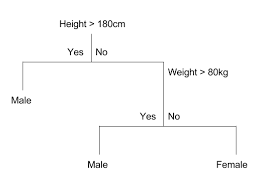
\includegraphics{CART.png} \centering
\captionof{figure}{Ejemplo de árbol de decisión. Fuente: Classification And Regression Trees for Machine Learning. Jason Brownlee, 2016}

\setlength\parskip{5ex}
\justifying

\noindent En este punto es cuando aparece el modelo de aprendizaje
automático llamado \texttt{Random\ Forest}. Este tipo de modelos superan
el problema explicado en el párrafo anterior entrenando múltiples
árboles de decisión en un subespacio del espacio formado por las
variables predictoras/explicativas, asumiendo como coste un ligero
incremento del sesgo. Esto significa que ninguno de los árboles del
bosque es entrenado con la totalidad de los datos de entrenamiento. Los
datos son recursivamente partidos en particiones, de manera que en un
nodo particular la partición se elabora haciendo una ``pregunta'' a una
de las variables. Por ejemplo, una partición podría estar hecha
``preguntándole'' a la variable \emph{Rate of Change 1 day} cuántos
datos tienen un valor superior/inferior a un cierto valor X. La elección
del criterio de partición de los datos se basa en alguna medida de
impureza tales como la Entropía de Shannon o la medida de impureza de
Gini. En el presente trabajo se utiliza la función \texttt{randomForest}
implementada en el paquete de R con el mismo nombre. Esta función
utiliza como medida de impureza a partir de la cual se particionan los
datos el índice de impureza de Gini (Liaw \& Wiener, 2002). Este índice
se utiliza como la función para medir la calidad de cada partición en
cada nodo. La impureza de Gini en el nodo N se calcula a partir de la
fórmula siguiente:

\[g(N)=\sum_{i\neq j}P(w_i)P(w_j)\]

\noindent Dónde \(P(w_i)\) es la proporción de casos donde la variable
respuesta toma la clase i. \(P(w_j)\) entonces es la propoción de casos
en los cuales la variable respuesta toma la clase j.

\noindent La manera heurística para escoger la mejor decisión de
particion en un nodo específico se basa en el hecho de conseguir la
mayor reducción posible de impureza. Es decir, la mejor partición
posible en un determinado nodo viene definida por la mayor ganancia de
información (variable que mejor particiona los datos / inclye más
observaciones en cada partición) o por la mayor reducción de impureza.
La ganancia de información que genera una determinada partición se puede
calcular con la fórmula siguiente:

\[\bigtriangleup I(N) = I(N) - P_L * I(N_L) - P_R*I(N_L)\]

\noindent Dónde \(I(N)\) es la medida de impureza (ya sea la impureza de
Gini o la entropía de Shannon) de un nodo \(N\). \(P_L\) es la
proporción de casos que en el nodo padre \(N\) van a parar al hijo
\textbf{izquierdo}. De un modo similar, \(P_R\) representa la proporción
de casos en el nodo padre \(N\) que se van a parar al nodo hijo
\textbf{derecho} después de realizar la partición. \(N_L\) y \(N_R\) son
los nodos hijos izquierdo y derecho, respectivamente.

\setlength\parskip{7ex}

\noindent Este tipo de modelos de aprendizaje automático son conocidos
como modelos \emph{ensemble}. En el núcleo de estos modelos está el
\emph{Bootstrap aggregating}, mayormente conocido como \emph{bagging}.
Esto significa que la predicción final se calcula como una media de la
solución obtenida con cada árbol construido sobre cada remuestra
generada con la técnica no paramétrica del \emph{bootstrap}. En otras
palabras: utilizando \emph{bootstrap} se calculan remuestras de los
datos con las cuales se contruye un árbol. Dentro de cada árbol
calculado sobre cada remuestra \emph{bootstrap} cada nodo es partido
utilizando la mejor variable dentro de la muestra de variables escogidas
aleatoriamente en cada nodo. Al final, la predicción del modelo es una
media de los valores obtenidos con todos estos árboles calculados sobre
las distintas remuestras \emph{bootstrap} (véase (Liaw \& Wiener, 2002)
p.~18 y (Dietterich, n.d.)). El método \emph{bagging} mejora la
estabilidad y la precisión de los algoritmos de aprendizaje. Al mismo
tiempo reduce la varianza y el sobreajuste, los cuales son un problema
relativamente común al construir árboles de decisión CART (véase
Luckyson Khaidem, 2016, p. 8 para un resumen del algoritmo escrito en
pseudocódigo).

\setlength\parskip{7ex}

\textbf{Modelos en h2o: AutoML}

\noindent En el apartado V.3 del presente trabajo se utiliza la función
\texttt{AutoML} del paquete \texttt{h2o} para hacer un análisis
automático sobre el modelo conceptual de predicción de la dirección de
movimiento del precio de cierre. Los modelos que esta función prueba son
los siguientes:

\begin{enumerate}
\def\labelenumi{\roman{enumi})}
\item
  \emph{Distributed Random Forest}. Este tipo de modelos incluyen tanto
  los modelos Random Forest descritos en el presente apartado como los
  modelos llamados Extremely Randomized Trees (Árboles aleatorizados de
  manera extrema). La diferencia entre este tipo de modelos (XRT) y los
  modelos Random Forest clásicos es que se añade otra capa de
  aleatoriedad en la manera en la que las particiones en cada nodo se
  calcula. Como en los Random Forest, se utiliza un subconjuto aleatorio
  de variables predictoras como candidatas en cada partición pero en vez
  de buscar el umbral que mejor discrimina (o parte) la base de datos,
  el umbral se construye aleatoriamente para cada variable candidata y
  el mejor de estos umbrales generados aleatoriamente se coge como la
  regla de partición. Esto normalmente permite reducir un poco más la
  varianza del modelo a expensas de un ligero incremento en el sesgo.
\item
  \emph{Generalized Linear Models}. Este tipo de modelos es ampliamente
  conocido. En este caso, al tratarse de un problema de clasificación,
  el modelo lineal generalizado que se prueba con la función
  \texttt{AutoML} es una regresión logística con variable respuesta
  binaria.
\item
  \emph{Extreme Gradient Boosting (Gradient Boosting Machine)}. Este
  tipo de modelos son considerados como modelos \emph{ensemble}.
  Consiste en construir árboles de clasificación de manera paralelizada
  para después hacer un \emph{ensemble} de ellos. Son en esencia modelos
  que se construyen por árboles de clasificación, cada uno construido
  con computación en paralelo.
\item
  \emph{DeepLearning (Fully-connected multi-layer artificial neural
  network)}. El modelo de deep learning que aplica el paquete \emph{h2o}
  está basado en una \emph{multi-layer feedforward artificial neural
  network} que se entrena utilizando el método de optimización llamado
  \emph{stochastic gradient descent} utilizando \emph{back-propagation}.
\item
  \emph{Stacked Ensemble}. El objetivo de los modelos \emph{ensemble} de
  machine learning es el de utilizar distintos modelos de aprendizaje
  automático para obtener un rendimiento mayor en cuanto a capacidad
  predictiva que la que podría obtener ninguno de los modelos
  individuales por si solo. De hecho, muchos de los modelos actuales de
  machine learning que se han vuelto populares son modelos
  \emph{ensemble}. Por ejemplo el mismo modelo Random Forest o las
  máquinas de gradientes potenciadas (Gradient Boosting Machine) son
  modelos \emph{ensemble} que utilizan métodos distintos para hacer este
  \emph{ensemble}. Los modelos Random Forest utilizan el método
  \emph{bagging (bootstrap aggregating)} mientras que los GBM utilizan
  el método del \emph{boosting}. Lo que permiten estos métodos es el
  coger un grupo de modelos más ``débiles'' (por ejemplo los árboles de
  decisión) para crear un único modelo más potente.
\end{enumerate}

\setlength\parskip{5ex}

\textbf{Long-Short Term Memory Recurrent Neural Network (LSTM)}

\noindent Este tipo de redes neuronales recurrentes, llamadas
simplemente LSTM, permiten resolver el problema que se planta con las
redes neuronales recurrentes tradicionales en cuanto a las dependencias
temporales alejadas en el tiempo. Las redes tradicionales presentan el
inconveniente de que no son capaces de recordar largas dependencias
temporales. Este tipo de redes, las LSTM, fueron introducidas por
Hochreiter \& Schmidhuber en 1997 y permiten solventar el problema de
las dependencias temporales grandes al permitir recordar información
durante largos periodos de tiempo. Para ayudar a la explicación de cómo
funcionan este tipo de redes neuronales se utilizan los gráficos creados
por (Olah, 2015), que utilizan una ilustración muy clara que permite una
explicación intuitiva de este tipo de modelos sin centrarse totalmente
en la formalidad matemática.

\noindent En primer lugar se presenta el esquema básico de una RNN LSTM.
Como todas las redes neuronales recurrentes se puede representar el
esquema como una cadena de módulos de red neuronal. La diferencia entre
las RNN clásicas y las LSTM es que su estructura interna es diferente ya
que tienen 4 redes neuronales internas en cada módulo en vez de una
simple capa.

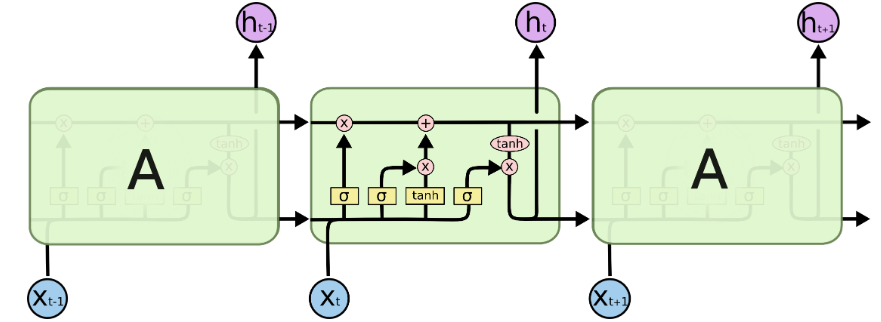
\includegraphics[width=6.25in,height=3.125in]{lstm1.png}
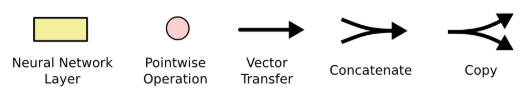
\includegraphics[width=5.20833in,height=0.83333in]{lstmlegend.png}
\centering
\captionof{figure}{Estructura general de una red neuronal recurrente LSTM. Fuente: (Olah, 2015)}

\setlength\parskip{5ex}
\justifying

\noindent La idea fundamental de este tipo de redes neuronales radica en
el llamado \emph{cell state} que en este caso está representado con la
línea que recorre la parte superior de la figura IV.3. Este \emph{cell
state} es el flujo de datos entre el módulo previo de la LSTM y el
módulo siguiente, y se ve afectado por la red LSTM que quita o añde
información a este flujo regulando este proceso a través de las
estructuras llamadas puertas o \emph{gates}. Estas puertas son redes
neuronales que deciden que cantidad de información previa va a afectar a
este flujo de datos o \emph{cell state}. Un módulo de LSTM tiene 4
puertas: 3 sigmoidales, que se encargan de decidir que porcentage de
información se mantiene y cuánto se olvida y una tanh que transforma el
rango de los valores entre -1 y 1.

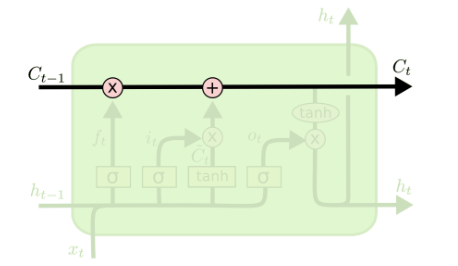
\includegraphics[width=4.42708in,height=2.08333in]{cellstate.png}
\centering
\captionof{figure}{Cell state. Cantidad de información que fluye a través de un módulo de la LSTM. Fuente: (Olah, 2015)}

\setlength\parskip{5ex}
\justifying

\hypertarget{primer-paso}{%
\paragraph{Primer paso}\label{primer-paso}}

\noindent El primer paso en la LSTM es decidir que información de
\(C_{t-1}\) se olvida, basado en \(h_{t-1}\) y \(x_t\). A esta puerta se
la conoce como la ``puerta del olvido'' y el proceso se elabora a través
de una capa sigmoidal, que decide qué partes de la información de
\(C_{t-1}\) hay que olvidar. Esta capa utiliza \(h_{t-1}\) y \(x_t\)
para sacar como output un valor entre 0 y 1 por cada número en el
\emph{cell state} \(C_{t-1}\). Un 1 representa ``recuerda totalmente
este elemento'' mientras que un 0 representa ``olvida totalmente este
elemento''.

\centering

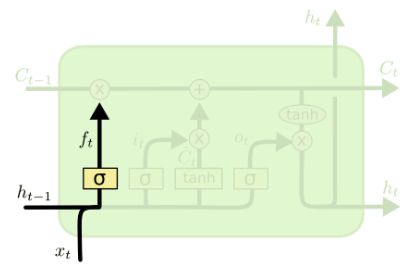
\includegraphics[width=6.25in,height=1.97917in]{firststeplstm.png}
\[f_t=\sigma \ (W_f \ \cdot \ [h_{t-1} \ , \ x_t] + b_f)\] \centering
\captionof{figure}{Primer paso o puerta en la LSTM. Fuente: (Olah, 2015)}

\setlength\parskip{5ex}
\justifying

\hypertarget{segundo-paso}{%
\paragraph{Segundo paso}\label{segundo-paso}}

\noindent En el segundo paso se decide qué nueva información se procede
a guardar en el \emph{cell state}. En primer lugar se encuentra una capa
sigmoidal llamada la ``puerta de entrada'' o ``\emph{input gate layer}''
que decide qué valores se procede a actualizar. A continuación una capa
con la función \textbf{tanh} crea un vector con los nuevos valores
candidatos \(\tilde{C_{t}}\) que pyede ser añadido al \emph{cell state}.
En otras palabras el proceso que tiene lugar en el segundo paso es el de
decidir que valores se van a actualizar y con que valor concreto lo van
a hacer. En el tercer paso se combinan estas dos puertas o capas para
actualizar el \emph{cell state}.

\centering

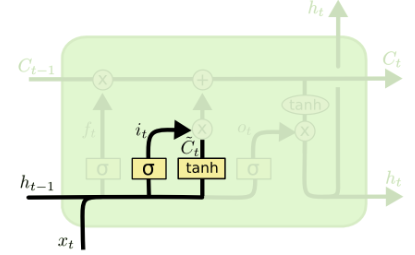
\includegraphics[width=6.25in,height=2.1875in]{secondsteplstm.png}
\[i_t = \sigma \ (W_i \ \cdot \ [h_{t-1} \ , \ x_t] + b_i)\]
\[\tilde{C}_t = tanh \ (W_C \ \cdot \ [h_{t-1} \ , \ x_t] + b_C)\]

\centering
  \captionof{figure}{Segundo paso en la LSTM. Puertas 2 y 3. Fuente: (Olah, 2015)}

\setlength\parskip{7ex}
\justifying

\hypertarget{tercer-paso}{%
\paragraph{Tercer paso}\label{tercer-paso}}

\noindent El tercer paso consiste en actualizar el antiguo \emph{cell
state}, o \(C_{t-1}\). En los pasos 1 y 2 ya se ha decidido qué
información olvidar y qué valores actualizar, junto con el valor
concreto que deben tener. Queda por tanto el trabajo de aplicar dichos
cambios. Se multiplica el antiguo \(C_{t-1}\) por \(f_t\), olvidando las
partes que se ha decidido previamente olvidar. Posteriormente se añade
\(i_t * \tilde{C_{t}}\), lo que crea los nuevos valores candidatos
escalador por el valor que indica cuánto se ha decidio actualizar cada
valor del \emph{cell state}.

\centering

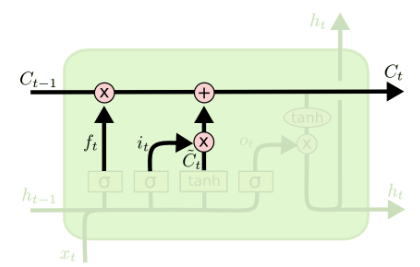
\includegraphics[width=6.25in,height=2.08333in]{thirdsteplstm.png}
\[C_t = f_t * C_{t-1} + i_t * \tilde{C}_t\]

\centering
  \captionof{figure}{Tercer paso en la LSTM. Aplicación de las puertas 1, 2 y 3. Fuente: (Olah, 2015)}

\setlength\parskip{5ex}
\justifying

\hypertarget{cuarto-paso}{%
\paragraph{Cuarto paso}\label{cuarto-paso}}

\noindent El cuarto y último paso consiste en decidir qué se va a
generar como \emph{output}. Este \emph{output} o resultado estará basado
en el \emph{cell state} pero será una versión filtrada del mismo. En
primer lugar se utiliza una capa sigmoidal la cual decide qué partes del
\emph{cell state} se sacarán como \emph{output}. Posteriormente se hace
pasar el \emph{cell state} a través de una capa \textbf{tanh} para
transformar los valores y ponerlos entre -1 y 1 y se multiplican por el
\emph{output} de la capa sigmoidal, de manera que sólo se sacan como
\emph{output} las partes que se deciden. De hecho, el proceso de
multiplicar la cantidad de memoria presente en el flujo que es
seleccionada por la capa \textbf{tanh} por la capa sigmoidal está
definiendo el volúmen de información que sale de la LSTM como output
hacia el siguiente módulo.

\centering

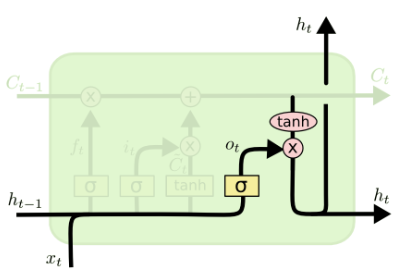
\includegraphics[width=6.25in,height=2.8125in]{laststeplstm.png}
\[o_t = \sigma \ (W_o \ \cdot \ [h_{t-1} \ , \ x_t] + b_o)\]
\[h_t=o_t * tanh(C_t)\]

\centering
  \captionof{figure}{Cuarto y último paso en la LSTM. Elección de la salida de la LSTM. Fuente: (Olah, 2015)}

\setlength\parskip{5ex}
\justifying

\noindent Finalmente cabe comentar que se construye una LSTM de tipo
\emph{STATEFULL}. Esto significa que todos los estados de la red son
propagados al siguiente \emph{batch}, de manera que no existe un proceso
de barajado interno sino que el estado de la muesta \(X_i\) será
utilizado en la computación de la muestra \(X_{i+bs}\) donde \(bs\) es
el tamaño del \emph{batch}.

\setlength\parskip{8ex}

\FloatBarrier
\fancyhead[L]{Métricas de rendimiento}
\fancyhead[R]{Capítulo \thechapter}
\fancyfoot[C]{\thepage}

\section{IV.2 \textbf{Métricas de rendimiento}}

\justifying

\hypertarget{modelos-de-clasificacion}{%
\paragraph{Modelos de clasificación}\label{modelos-de-clasificacion}}

\setlength\parskip{6ex}

\noindent Los modelos construidos están pensados para ser de ayuda a la
hora de tomar una decisión de compra o venta de un \emph{stock}. Si la
predicción es +1 (Up) se espera que el precio al cabo de
\(d=30, \ 60 \ y \ 90\) días sea superior al actual y entonces la acción
lógica del inversor sería \textbf{comprar}. Al contrario ocurriría si la
predicción fuera -1, lo cual significaría que se espera que el precio al
cabo de \(d\) días sea inferior. En este caso la decisión razonable a
tomar por parte del inversor sería \textbf{vender}. Una predicción
errónea puede causar grandes perdidas de dinero para el inversor. Por lo
tanto, se deben definir métricas que ayuden a evaluar la potencia
predictiva de los modelos construidos. Las métricas que se utilizan en
el presente trabajo para evaluar el rendimiento de los modelos de
clasificación que se crean a continuación son las siguientes:

\setlength\parskip{9ex}

\emph{Accuracy}

\noindent Esta métrica hace referencia a la proporción de casos
clasificados correctamente entre el total de casos con los que se prueba
el modelo. Se calcula a partir de la fórmula siguiente:

\[Accuracy = \frac{tp+tn}{tp+tn+fp+fn} \ \ \ \ \ \ \ \ \ \ \ \ \ \ (M.1)\]

\emph{Recall/Sensitivity}

\noindent Esta métrica mide la habilidad de un modelo clasificador de
identificar correctamente los casos positivos.

\[Sensitivity = \frac{tp}{tp+fn} \ \ \ \ \ \ \ \ \ \ \ \ \ \ (M.2)\]

\emph{Specificity}

\noindent Esta métrica mide la habilidad de un modelo clasificador de
identificar correctamente los casos negativos.

\[Specificity = \frac{tn}{tn+fp} \ \ \ \ \ \ \ \ \ \ \ \ \ \ (M.3)\]

\noindent Dónde,

\setlength\parskip{5ex}

\noindent tp = número de verdaderos positivos \(\equiv\) número de veces
en las que el caso era positivo y el modelo predice positivo

\noindent tn = número de verdaderos negativos \(\equiv\) número de veces
en las que el caso era negativo y el modelo predice negativo

\noindent fp = número de falsos positivos \(\equiv\) número de veces en
las que el caso era negativo y el modelo predice positivo

\noindent fn = número de falsos negativos \(\equiv\) número de veces en
las que el caso era positivo y el modelo predice negativo

\emph{Area Under the Curve (AUC)}

\noindent Directamente derivado de la curva ROC se define este
estadístico llamado Área bajo la curva. Como su nombre indica, se trata
de calcular el área que queda por debajo de la curva ROC. El objetivo de
esta métrica es el de calcular los distintos ratios de verdaderos
positivos y de falsos positivos para distintos umbrales definidos, no
sólo para el umbral de 0.5 de probabilidad. La idea es que de un
clasificador aleatorio se puede obtener tantos verdaderos positivos como
falsos positivos, que es lo que indica un AUC de 0.5 o la recta y=x en
la curva ROC. Por lo tanto, el AUC indica la capacidad del modelo
clasificador de obtener más verdaderos positivos que falsos positivos
para todos los umbrales posibles. Como se ha indicado, un AUC de 1
indicaria un modelo clasificador perfecto, capaz de predecir con un
100\% de acierto los verdaderos positivos y de no dar ningún falso
positivo mientras que un AUC de 0.5 indicaria el mismo número de falsos
positivos que de verdaderos positivos. El objetivo es, pues, el de
obtener un modelo clasificador que tengo un AUC entre 0.5 y 1 cosa que
significa que puede mejorar la predicción aleatoria. Otro de los usos
comunes de esta métrica es la de poder comparar modelos clasificadores
de manera que un mismo modelo será mejor que otro si su AUC es mayor.

\setlength\parskip{7ex}

\noindent La diferencia básica respecto a la \emph{accuracy} definida en
M.1 es que para calcular la \emph{accuracy} el usuario tiene que definir
un umbral a partir del cual se define la clasificación como ``1'' o
``0'' (caso positivo o negativo) mientras que el AUC está midiendo el
rendimiento del modelo \textbf{mientras el umbral varía sobre todo los
posibles valores}. En este sentido el AUC es una métrica más general que
no depende (no es función de) el umbral que se defina.

\setlength\parskip{5ex}

\hypertarget{modelos-de-regresion}{%
\paragraph{Modelos de regresión}\label{modelos-de-regresion}}

\noindent Para la evaluación de la LSTM sobre los precios se utilizan
las siguientes métricas:

\emph{MAPE}

\noindent Conocido por sus siglas en inglés, el Mean Absolute Percentage
Error representa el error medio percentual que obtenemos al hacer una
predicción. Se calcula de la siguiente manera:

\[MAPE = \frac{1}{n}\sum_{i=1}^{n}\frac{\left |  Actual_i \ -\ Predicted_i\right |}{Actual_i} \ \ \ \ \ \ \ \ \ \ \ \ \ \ (M.4)\]

\noindent  A su vez también se propone una medida alternativa de MAPE,
que ofrece una visión más compensada de los errores:

\[MAPE_2 = \frac{\sum_{i=1}^{n}\left |  Actual_i \ -\ Predicted_i\right |}{\sum_{i=1}^{n}Actual_i} \ \ \ \ \ \ \ \ \ \ \ \ \ \ (M.5)\]

\noindent Paralelamente a la medida de MAPE, cuyo rango de valores está
restringido entre 0 y 1, se presentan las siguientes dos métricas:

\[MAE = \frac{1}{n}\sum_{i=1}^{n}\left |  Actual_i \ -\ Predicted_i\right | \ \ \ \ \ \ \ \ \ \ \ \ \ \ (M.6)\]
\setlength\parskip{5ex}

\[RMSE = \sqrt{\frac{1}{n}\sum_{i=1}^{n}(Actual_i \ -\ Predicted_i)^2} \ \ \ \ \ \ \ \ \ \ \ \ \ \ (M.7)\]

\FloatBarrier
\newpage
\fancyhead[L]{CASOS PRÁCTICOS: EJECUCIÓN}
\fancyhead[R]{\thepage}
\fancyfoot[C]{}

\chapter{\textbf{CASOS PRÁCTICOS: EJECUCIÓN}}
\justifying

\FloatBarrier
\fancyhead[L]{Dirección de movimiento del precio: análisis detallado con Random Forest}
\fancyhead[R]{\thepage}
\fancyfoot[C]{}

\section{V.1 \textbf{Dirección de movimiento del precio de cierre: análisis detallado con Random Forest}}

\noindent En el apartado siguiente se elabora la primera aplicación
práctica de un sistema de inteligencia artificial sobre el sector de la
inversión en activos financieros. En este apartado se procede a
desarrollar un sistema clasificador que sea capaz de predecir la
dirección del movimiento de un determinado \emph{stock}. Concretamente,
el objetivo de este tipo de aplicación es el de desarrollar un sistema
que sea capaz de predecir si el precio de cierre de un activo será mayor
o inferior al del momento actual al cabo de una determinada ventana de
tiempo.

\noindent Se estructura la sección de la manera siguiente: en primer
lugar se explica la procedencia y se describe la base de datos
utilizada. En segundo lugar se explican los tratamientos de
procesamiento de los datos que se aplican sobre los datos sucios
extraídos previamente. A continuación se describen detalladamente los
procesos de creación de variables que se elaboran para poder utilizarlas
como \emph{inputs} del modelo. En última instancia se propone una
partición sobre los datos, previa a la realización de los experimentos y
al análisis de los resultados.

\FloatBarrier
\fancyhead[L]{Base de datos: Obtención y descripción}
\fancyhead[R]{Sección V.1}
\fancyfoot[C]{\thepage}

\subsection{V.1.1 \textbf{Base de datos: Obtención y descripción}}

\hypertarget{obtencion}{%
\paragraph{Obtención}\label{obtencion}}

\noindent Los datos con los que se va a realizar la modelización
descrita en este apartado se obtienen a través del paquete
\texttt{quantmod}. Este paquete se diseñó para assistir a los
\emph{traders} quantitativos en el desarrollo, evaluación y puesta en
funcionamiento de modelos de \emph{trading} basados en la estadística.
Concretamente, se utiliza la función \texttt{getSymbols} para obtener
los datos ya que permite cargar y manejar \texttt{Symbols} en un
ambiente especificado. Las posibles fuentes de datos son: Yahoo; Google,
aunque actualmente no funciona; Alphavantage, con la ventaja de que
podemos obtener datos intra-dia; MySQL, FRED, etc. Para obtener los
datos se procede a utilizar \emph{Yahoo Finance} como la fuente.

\setlength\parskip{5ex}

\noindent La metodología para la búsqueda de los distintos stocks con
los cuales entrenar los modelos predictivos empieza con la idea de
querer encontrar empresas representativas dentro de distintos sectores
estratégicos y con amplio impacto en la economía real. Además se
pretende que los stocks utilizados tengan rentabilidad financiera con el
objetivo de llevar el presente trabajo lo más cerca posible de una
situación real de inversión. Para ello se utiliza el portfolio a fecha
01/01/2019 del gran \emph{gurú} de las finanzas Warren Buffet
(\emph{Warren buffett}, n.d.). Dentro de las numerosas empresas
presentes en este portfolio se escogen los 3 \emph{stocks} del NYSE
(bolsa de nueva york) y una del NASDAQ.

\begin{table}[H]
\centering\begingroup\fontsize{10}{12}\selectfont

\begin{tabular}{l|l|l}
\hline
Simbolo & Nombre & Bolsa\\
\hline
AAPL & Apple Inc. & NASDAQ\\
\hline
WFC & Wells Fargo \& CO & NYSE\\
\hline
KO & Coca-Cola Company & NYSE\\
\hline
AXP & American Express CO & NYSE\\
\hline
\end{tabular}
\endgroup{}
\end{table}
\centering
  \captionof{table}{Stocks utilizados}

\setlength\parskip{7ex}
\justifying

\noindent Al hecho de que los \emph{stocks} que forman la base de datos
formen parte del portfolio de uno de los \emph{gurús} del mundo de las
finanzas y la inversión, se le suma también el hecho de que las empresas
escogidas son empresas multinacionales con un gran capital que ocupan
una posición destacada sus respectivos mercados, siendo representativas
de cada uno de los sectores en los cuales operan. Seguidamente se
describen brevemente las actividades de las cuatro compañías, siendo
éstas el sector retail, sector tecnológico y sector de los servicios
financieros o banca.

\textbf{Coca - Cola Company}

\noindent The Coca-Cola Company es una empresa multinacional de bebidas
estadounidense. Tiene su sede en Atlanta, Georgia y es conocida por
comercializar el refresco más consumido del mundo: la Coca-Cola. Esta
bebida azucarada se creó en 1886 y forma parte de la historia moderna
del mundo. Actualmente esta compañía está considerada una de las más
grandes corporaciones de EEUU.

\textbf{Apple INC.}

\noindent Apple, Inc.~es una empresa estadounidense del sector
tecnológico que diseña y produce equipos electrónicos, software y
hardware y ofrece servicios en línea. Es una compañía multinacional de
gran renombre y trascendencia en los últimos años al ser los creadores
del iPhone, el famoso teléfono inteligente, así como el ordenador
personal Mac o el reproductor de música iPod. También ofrece el
desarrollo de su propio sistema operativo que está presente en todos sus
productos.

\textbf{American Express}

\noindent American Express Company (NYSE AXP) es una empresa dedicada a
los servicios de finanzas, entre los cuales destaca la emisión de una
tarjeta de crédito que lleva su mismo normbre y que es bastante popular
en estados unidos. Esta compañía fue fundada en 1850.

\textbf{Wells Fargo \& Company}

\noindent Wells Fargo \& Co.~es una compañía de servicios financieros
que opera a nivel internacional. Se trata de uno de los bancos más
importantes en los Estados Unidos, considerándose entre los 4 más
potentes. Tiene su sede en California y es el resultado de una
adquisición por parte de Norwest Corporation de Californa Wells Fargo \&
Co.~en el año 1998.

\hypertarget{descripcion}{%
\paragraph{Descripción}\label{descripcion}}

\noindent Después de utilizar la función \texttt{getSymbols} se obtiene
una tabla para cada stock con un formato estandarizado. Se obtienen 5
series temporales con periodicidad diaria que hacen referencia a los
precios de \textbf{apertura}, \textbf{cierre}, \textbf{máximo},
\textbf{mínimo} y \textbf{volúmen}. Además se incluye el precio ajustado
pero esta variable no será utilizada en este trabajo. Todas las
variables presentes en la base de datos utilizada son numéricas.

\setlength\parskip{5ex}
\justifying

\noindent Los datos utilizados en este trabajo compreden el período 2000
- 2018, siendo el día \texttt{2000-01-01} la primera observación de cada
serie temporal. La última observación de la base de datos es
\texttt{2018-12-31}.

\setlength\parskip{5ex}
\justifying

\noindent La función \texttt{str} permite visualizar fácilmente la
estructura y formato que presentan en R las distintas tablas de la base
de datos inicial. En el siguiente output se muestra como ejemplo la
empresa Coca-Cola Company.

\centering

\begin{verbatim}
## 'data.frame':    4778 obs. of  6 variables:
##  $ KO.Open    : num  29 28.2 28.2 28.5 28.9 ...
##  $ KO.High    : num  29 28.4 28.7 28.8 30.4 ...
##  $ KO.Low     : num  27.6 27.8 28 28.3 28.9 ...
##  $ KO.Close   : num  28.2 28.2 28.5 28.5 30.4 ...
##  $ KO.Volume  : num  10997000 7308000 9457400 7129200 11474000 ...
##  $ KO.Adjusted: num  12.3 12.3 12.4 12.4 13.2 ...
\end{verbatim}

\setlength\parskip{5ex}
\justifying

\emph{Tablas descriptivas}

\noindent Se explora descriptivamente los datos analizando los
estadísticos descriptivos . Para cada empresa, se obtienen los distintos
estadísticos de cada una de las variables descritas previamente. Para
ello se elaboran 4 tablas que hacen referencia a los distintos
estadísticos, calculados sobre los distintos precios y el volúmen, para
una misma empresa.

\begin{table}[H]
\centering\begingroup\fontsize{10}{12}\selectfont

\begin{tabular}{l|l|l|l|l|l|l}
\hline
  & Min. & 1st Qu. & Median & Mean & 3rd Qu. & Max.\\
\hline
Open & 18.55 & 23.49 & 28.75 & 31.43 & 40.4 & 50.82\\
\hline
High & 18.8 & 23.72 & 29.01 & 31.66 & 40.6 & 50.84\\
\hline
Low & 18.5 & 23.26 & 28.47 & 31.19 & 40.15 & 50.25\\
\hline
Close & 18.54 & 23.5 & 28.77 & 31.44 & 40.39 & 50.51\\
\hline
Volume & 2.147M & 9.821M & 12.972M & 14.692M & 17.49M & 124.169M\\
\hline
\end{tabular}
\endgroup{}
\end{table}
  \captionof{table}{Estadísticos descriptivos para los distintos precios de Coca-Cola Company}

\setlength\parskip{5ex}
\justifying

\noindent Como se puede apreciar en la tabla V.2 el rango que han tomado
los precios de cierre para la empresa Coca-Cola CO. en el período
estudiado se mueve entre 18.54 y 50.51. El precio medio de cierre para
el período estudiado es de 31.44 dólares.

\begin{table}[H]
\centering\begingroup\fontsize{10}{12}\selectfont

\begin{tabular}{l|l|l|l|l|l|l}
\hline
  & Min. & 1st Qu. & Median & Mean & 3rd Qu. & Max.\\
\hline
Open & 0.93 & 4.37 & 26.13 & 51.65 & 90.52 & 230.78\\
\hline
High & 0.94 & 4.47 & 26.53 & 52.13 & 91.37 & 233.47\\
\hline
Low & 0.91 & 4.21 & 25.66 & 51.12 & 89.72 & 229.78\\
\hline
Close & 0.94 & 4.36 & 26.1 & 51.64 & 90.52 & 232.07\\
\hline
Volume & 9.835M & 52.133M & 93.003M & 119.542M & 156.041M & 1855.41M\\
\hline
\end{tabular}
\endgroup{}
\end{table}
  \captionof{table}{Estadísticos descriptivos para los distintos precios de Apple Inc.}

\setlength\parskip{5ex}
\justifying

\noindent Como se puede apreciar en la tabla V.3 el rango que han tomado
los precios de cierre para la empresa Apple Inc.~en el período estudiado
se mueve entre 0.94 y 232.07. El precio medio de cierre para el período
estudiado es de 51.64 dólares, superior al de la empresa Coca-Cola CO.

\begin{table}[H]
\centering\begingroup\fontsize{10}{12}\selectfont

\begin{tabular}{l|l|l|l|l|l|l}
\hline
  & Min. & 1st Qu. & Median & Mean & 3rd Qu. & Max.\\
\hline
Open & 9.99 & 41.14 & 50.19 & 55.59 & 69.94 & 113.99\\
\hline
High & 10.66 & 41.58 & 50.89 & 56.16 & 70.45 & 114.55\\
\hline
Low & 9.71 & 40.5 & 49.72 & 55 & 69.56 & 112\\
\hline
Close & 10.26 & 41.04 & 50.22 & 55.59 & 70.08 & 112.89\\
\hline
Volume & 0.837M & 3.85M & 5.314M & 6.979M & 7.965M & 90.337M\\
\hline
\end{tabular}
\endgroup{}
\end{table}
  \captionof{table}{Estadísticos descriptivos para los distintos precios de American Express CO.}

\setlength\parskip{5ex}
\justifying

\noindent Como se puede apreciar en la tabla V.4 el rango que han tomado
los precios de cierre para la American Express CO. en el período
estudiado se mueve entre 10.26 y 112.89. El precio medio de cierre para
el período estudiado es de 55.59 dólares, ligeramente superior al de la
empresa Apple Inc..

\begin{table}[H]
\centering\begingroup\fontsize{10}{12}\selectfont

\begin{tabular}{l|l|l|l|l|l|l}
\hline
  & Min. & 1st Qu. & Median & Mean & 3rd Qu. & Max.\\
\hline
Open & 8.65 & 25.95 & 31.19 & 35.19 & 45.82 & 65.89\\
\hline
High & 8.94 & 26.29 & 31.48 & 35.56 & 46.23 & 66.31\\
\hline
Low & 7.8 & 25.54 & 30.84 & 34.82 & 45.47 & 65.66\\
\hline
Close & 8.12 & 25.91 & 31.2 & 35.2 & 45.97 & 65.93\\
\hline
Volume & 1.774M & 9.129M & 15.235M & 23.412M & 27.088M & 478.737M\\
\hline
\end{tabular}
\endgroup{}
\end{table}
  \captionof{table}{Estadísticos descriptivos para los distintos precios de Wells Fargo and CO.}

\setlength\parskip{5ex}
\justifying

\noindent Como se puede apreciar en la tabla V.5 el rango que han tomado
los precios de cierre para la empresa Wells Fargo and CO. en el período
estudiado se mueve entre 8.12 y 65.93. El precio medio de cierre para el
período estudiado es de 35.2 dólares, ligeramente superior al de
Coca-Cola CO. inferior al de \texttt{AAPL} y \texttt{AXP}.

\emph{Visualización gráfica}

\noindent Seguidamente se explora gráficamente el precio de cierre para
cada una de las empresas, al ser éste la variable a partir de la cual se
calculará la variable respuesta sobre la que hacer predicción. El
objetivo de este tipo de análisis es poder visualizar el tipo de
evolución que han presentado los distintos \emph{stocks} durante el
período de estudio.

\setlength\parskip{5ex}
\justifying

\noindent En el siguiente gráfico se representa el precio de cierre de
Coca-Cola Company para el período comprendido entre el 03/01/2000 y
28/12/2018.

\begin{center}\includegraphics{figures/unnamed-chunk-31-1} \end{center}
  \captionof{figure}{Precio de cierre de Coca-Cola Company 03/01/2000 - 28/12/2018}

\setlength\parskip{5ex}
\justifying

\noindent En el siguiente gráfico se representa el precio de cierre de
Apple Inc.~para el período comprendido entre el 03/01/2000 y 28/12/2018.

\begin{center}\includegraphics{figures/unnamed-chunk-32-1} \end{center}
  \captionof{figure}{Precio de cierre de Apple Inc. 03/01/2000 - 28/12/2018}

\setlength\parskip{5ex}
\justifying

\noindent En el siguiente gráfico se representa el precio de cierre de
Wells Fargo and CO. para el período comprendido entre el 03/01/2000 y
28/12/2018.

\begin{center}\includegraphics{figures/unnamed-chunk-33-1} \end{center}
\centering
  \captionof{figure}{Precio de cierre de American Express CO. 03/01/2000 - 28/12/2018}

\setlength\parskip{5ex}
\justifying

\noindent En el siguiente gráfico se representa el precio de cierre de
Wells Fargo and CO. para el período comprendido entre el 03/01/2000 y
28/12/2018.

\begin{center}\includegraphics{figures/unnamed-chunk-34-1} \end{center}
\centering
  \captionof{figure}{Precio de cierre de Wells Fargo and CO. 03/01/2000 - 28/12/2018}

\setlength\parskip{5ex}
\justifying

\noindent A partir de esta exploración gráfica se descubre que 3 de las
4 empresas (KO, AXP y WFC) presentan un comportamiento relativamente
similar. Como se puede observar en la figura V.1, V.3 y V.4 la evolución
de \texttt{KO,\ AXP\ y\ WFC} en el período estudiado presenta una
tendencia, en general, creciente. Si se analiza en detalle el lector
puede detectar 3 etapas claramente destacada en la evolución de estos
stocks, siendo la primera de ellas distinta en el caso de Wells Fargo \&
CO. Estos 3 períodos claramente diferenciados son los correspondientes a
los años 2000-2007, 2008-2010 y 2011-2018.

\textbf{2000-2006}

\noindent En el caso de las empresas Coca-Cola CO. y American Express
CO. la primera etapa (2000 - inicios de 2006) corresponde a la
relajación de los mercados financieros posterior al \emph{boom de las
.com}. La segunda mitad de los 90 fueron una época de expansión
económica en la cual se produjo un boom financiero en USA (ver Urban
Jermann, 2003) que se relajó a partir de finales de milenio.

\textbf{2006-2008}

\noindent Esta relajación fué seguida por la segunda etapa, un período
de crecimiento económico y de los mercados financieros que se produjo a
partir del 2006 y hasta el 2008. Esta etapa de crecimiento fué previa a
la gran recesión mundial que tuvo lugar a partir del año 2008 (ver
(Andrew K. Rose, 2011), (DeLong, 2009), (P.R. Lane, 2011) pp.~77-110
para más información{]}.

\textbf{2008-2010}

\noindent Posterior al crecimiento experimentado a nivel global antes
del año 2008, se produjo la última gran crisis financiera que ha tenido
lugar a nivel global. Es bien sabido que el problema financiero que se
expandió a Europa empezó en USA, a causa de los paquetes de activos
financieros de alto riesgo mezclados con otro tipo de activos
financieros. Esta crisis se ve representada en los gráficos gracias al
socavón que presentan los precios de cierre de las empresas consideradas
como ejemplo entre el 2008 y el 2010. Cabe destacar que ,como se puede
apreciar a partir de las gráficas anteriores, la empresa Apple Inc.~es
la única empresa de las 4 consideradas como ejemplo que no fue
fuertemente afectada durante este periodo de crisis, experimentando sus
precios un ligero decremento durante este periodo (ligero en comparación
con las otras empresas).

\textbf{2010 - Actualidad}

\noindent La etapa posterior a la gran crisis financiera mundial del
2008-2010 ha sido una etapa de crecimiento, tal como demuestra el hecho
de que las 4 empresas consideradas presentan un crecimiento de los
precios de cierre. Especialmente en Europa, a partir de las políticas de
austeridad creadas después de la crisis, lideradas por Alemania,
permitieron una situación económica favorable para el crecimiento, al
mantener el BCE el precio del dinero (el tipo de interés) prácticamente
al nivel de 0.

\setlength\parskip{5ex}
\justifying

\emph{Descriptiva financiera}

\noindent Seguidamente se muestran las distintas tablas comparativas de
los distintos precios obtenidos inicialmente. Éstas incluyen la media,
la desviación típica o volatilidad del precio y el coeficiente de
variación, el cual es un estadístico utilizado de manera frecuente para
medir la volatilidad de un stock al ser una variable que no tiene en
cuenta las unidades de medida. Esto significa que permite comparar
distintos stocks en cuanto a volatilidad se refiere sin tener en cuenta
la magnitud que éstos presenten.

\noindent Este tipo de visualización permite analizar más detenidamente
cada uno de los precios y poder compararlos fácilmente entre todas las
empresas. Es además una buena manera de analizar a priori la
predictibilidad de los distintos precios al poder comparar los distintos
coeficientes de variación. La idea de evaluar la predictibilidad de una
serie temporal con el coeficiente de variación sugiere que es más fácil
de predecir una serie temporal con un comportamiento más estable, esto
es, con menos unidades de desviación típica por unidad de media
(Gilliland, 2009).

\begin{table}[H]
\centering\begingroup\fontsize{10}{12}\selectfont

\begin{tabular}{l|r|r|r}
\hline
Nombre & Media & Desv\_std & CoV\\
\hline
Apple Inc. & 51.64595 & 55.925416 & 1.0828616\\
\hline
Wells Fargo \& CO & 35.19440 & 11.806917 & 0.3354771\\
\hline
Coca-Cola Company & 31.42690 & 8.652774 & 0.2753302\\
\hline
American Express CO & 55.58608 & 21.112421 & 0.3798149\\
\hline
\end{tabular}
\endgroup{}
\end{table}
\centering
  \captionof{table}{Estadísticos descriptivos para el precio de apertura (Open).}

\begin{table}[H]
\centering\begingroup\fontsize{10}{12}\selectfont

\begin{tabular}{l|r|r|r}
\hline
Nombre & Media & Desv\_std & CoV\\
\hline
Apple Inc. & 52.13167 & 56.386960 & 1.0816258\\
\hline
Wells Fargo \& CO & 35.56184 & 11.819827 & 0.3323739\\
\hline
Coca-Cola Company & 31.66443 & 8.670834 & 0.2738351\\
\hline
American Express CO & 56.16119 & 21.131090 & 0.3762579\\
\hline
\end{tabular}
\endgroup{}
\end{table}
\centering
  \captionof{table}{Estadísticos descriptivos para el precio máximo (High).}

\begin{table}[H]
\centering\begingroup\fontsize{10}{12}\selectfont

\begin{tabular}{l|r|r|r}
\hline
Nombre & Media & Desv\_std & CoV\\
\hline
Apple Inc. & 51.12417 & 55.450009 & 1.0846143\\
\hline
Wells Fargo \& CO & 34.82003 & 11.805231 & 0.3390357\\
\hline
Coca-Cola Company & 31.18907 & 8.644319 & 0.2771585\\
\hline
American Express CO & 55.00056 & 21.083165 & 0.3833264\\
\hline
\end{tabular}
\endgroup{}
\end{table}
\centering
  \captionof{table}{Estadísticos descriptivos para el precio mínimo (Low).}

\begin{table}[H]
\centering\begingroup\fontsize{10}{12}\selectfont

\begin{tabular}{l|r|r|r}
\hline
Nombre & Media & Desv\_std & CoV\\
\hline
Apple Inc. & 51.63773 & 55.925371 & 1.0830331\\
\hline
Wells Fargo \& CO & 35.19502 & 11.807079 & 0.3354758\\
\hline
Coca-Cola Company & 31.43855 & 8.656529 & 0.2753476\\
\hline
American Express CO & 55.58724 & 21.099819 & 0.3795803\\
\hline
\end{tabular}
\endgroup{}
\end{table}
\centering
  \captionof{table}{Estadísticos descriptivos para el precio de cierre (Close).}

\setlength\parskip{5ex}
\justifying

\noindent Como se puede apreciar en la tabla V.9, las compañías American
Express y Apple Inc.~son las que presentan un precio de cierro medio
mayor, superando en ambos casos los 50 dólares/acción. A su vez son las
2 compañías que presentan una desviación estándard del precio de cierre
mayor, siendo la de Apple la mayor de todas con 55.93. Esto se debe al
hecho de que Apple presenta una gran tendencia creciente en los precios
de cierre desde el año 2000 y el cálculo de la desviación estándard no
es capaz de eliminar este efecto de la tendencia. Este hecho también se
aprecia en el cálculo del coeficiente de variación, que en el caso de
Apple es superior a 1. Por otro lado, la empresa que presenta unos
resultados menores es Coca-Cola CO., con un menor precio de cierre medio
(31.44dólares/acción) y menores desviación típica y coeficiente de
variación.

\setlength\parskip{5ex}
\begin{table}[H]
\centering\begingroup\fontsize{10}{12}\selectfont

\begin{tabular}{l|r|r}
\hline
Nombre & Media & Varianza\\
\hline
Apple Inc. & 0.077 & 7.203\\
\hline
Wells Fargo \& CO & 0.018 & 5.699\\
\hline
Coca-Cola Company & 0.011 & 1.679\\
\hline
American Express CO & 0.015 & 5.004\\
\hline
\end{tabular}
\endgroup{}
\end{table}
\centering
  \captionof{table}{Momentos calculados sobre los logaritmos de la rentabilidad (*log returns*)}

\setlength\parskip{5ex}
\justifying

\noindent En la tabla anterior se muestra la media y la varianza de las
rentabilidades de las distintas empresas durante el periodo estudiado.
La empresa que ofrece una mayor rentabilidad media es Apple, pero a su
vez presenta una mayor varianza. En este sentido las empresas Wells
Fargo y American Express no parecen tan recomendables al presentar
rentabilidades medias de menos del 0.02\% y varianzas de más de 5
puntos. Esto significa que estos stocks aportan, de media, unas
rentabilidades relativamente bajas en comparación con el riesgo que
habría que asumir. En este caso una opción más balanceada en términos de
rentabilidad-riesgo es la de Coca-Cola ya que tiene una rentabilidad
media de 0.01\% con un riesgo de 1.7.

\setlength\parskip{5ex}
\justifying

\FloatBarrier
\fancyhead[L]{Procesamiento de los datos}
\fancyhead[R]{Sección V.1}
\fancyfoot[C]{\thepage}

\subsection{V.1.2 \textbf{Procesamiento de los datos}}

\noindent Siguiendo la metodología propuesta en la figura 2.1, en primer
lugar se procede a elaborar una transformación de todas las
variables/precios iniciales. Esta transformación suaviza los datos con
el objetivo de remover la variación aleatória y/o el ruido, haciendo que
los modelos predictivos de dirección de movimiento elaborados
posteriormente sean capaces de detectar más fácilmente una tendencia a
largo plazo de los precios dentro del comportamiento de los mismos
(Luckyson Khaidem, 2016, p. 4). El objetivo es, por un lado, crear la
variable respuesta utilizando el precio de cierre alisado y, por otro,
calcular los indicadores técnicos detallados en la sección 5.3 para,
posteriormente, utilizarlos como variables predictoras.

\setlength\parskip{7ex}

\noindent Por un lado se utilizan las medias móviles exponenciales a 30,
60 y 90 días como nuevas representaciones de los precios. De esta manera
se obtiene una nueva representación de los precios en la cual se ha
removido la variación aleatória y el ruido. Seguidamente se muestran las
gráficas para las medias móviles exponenciales del precio de cierre para
la empresa Coca-Cola CO. con el objetivo de visualizar el alisado que se
obtiene al aplicar este cálculo. A medida que se añaden más datos en el
cálculo de las medias se obtiene un mayor alisado.

\justifying

\noindent Por otro lado se aplica el mismo tipo de alisado exponencial
aplicado por (Luckyson Khaidem, 2016, p. 4). El objetivo es el mismo que
en el caso del cálculo de las medias móviles. El estadístico alisado
exponencialmente de un serie temporal \(Y\) se puede calcular
recursivamente, desde el momento en el que se disponga de dos
observaciones, de la manera siguiente:

\setlength\parskip{5ex}

\[ S_0 = Y_o \]
\[ S_t = \alpha*Y_y+(1-\alpha)*S_{t-1} \ \ \ \ \forall \ \ t>0 \ \ \ \ \ \ \ \ \ \ \ \ \ \ \ \ (1)\]

\setlength\parskip{8ex}

\noindent donde \(0 < \alpha < 1\) es el factor de alisado. El método
del alisado exponencial otorga más peso a las observaciones más
recientes en tanto que hace decrecer exponencialmente el peso de las
observaciones más antiguas. (cita articulo, formula internet). Valores
elevados de \(\alpha\) provocan que el nivel de alisado quede reducido,
de manera que en el caso extremo en el que \(\alpha=1\) el estadístico
exponencialmente alisado es igual que la observación. Es decir
\(S_t=Y_t \ \ \ \ si \ \alpha=1\). En el presente trabajo se aplica la
fórmula anterior sobre cada uno de los precios y el volúmen con un
factor de alisado \(\alpha=0.05\) para conseguir un alisado más
pronunciado que en el caso de las medias móviles exponenciales.

\justifying

\noindent A su vez se presentan la siguiente tabla para poder visualizar
la disminución de variabilidad que se obtiene tras aplicar las distintas
medias móviles exponenciales al precio de cierre de las distintas
empresas. La volatilidad se evalúa en este caso con el coeficiente de
variación para permitir la comparabilidad:

\begin{table}[H]
\centering\begingroup\fontsize{10}{12}\selectfont

\begin{tabular}{l|r|r|r|r}
\hline
Nombre & CoV\_EMA30 & CoV\_EMA60 & CoV\_EMA90 & CoV.exp.smooth.alpha.0.05\\
\hline
Apple Inc. & 1.0799103 & 1.0746436 & 1.0686425 & 1.0852714\\
\hline
Wells Fargo \& CO & 0.3322648 & 0.3290268 & 0.3263450 & 0.3336280\\
\hline
Coca-Cola Company & 0.2735308 & 0.2716672 & 0.2700638 & 0.2722442\\
\hline
American Express CO & 0.3763897 & 0.3725283 & 0.3686093 & 0.3746762\\
\hline
\end{tabular}
\endgroup{}
\end{table}
  \captionof{table}{Comparativa coeficiente de variación entre las distintas medias móviles exponenciales}

\setlength\parskip{5ex}
\justifying

\noindent Una vez alisados los precios de los distintos \emph{stocks} se
procede a calcular tanto la variable respuesta como las variables
predictoras, en este caso los indicadores técnicos, a partir de éstos.

\FloatBarrier
\fancyhead[L]{Creación de variables}
\fancyhead[R]{Sección V.1}
\fancyfoot[C]{\thepage}

\subsection{V.1.3 \textbf{Creación de variables}}

\setlength\parskip{5ex}

\hypertarget{variable-respuesta}{%
\paragraph{Variable respuesta}\label{variable-respuesta}}

\noindent Después de aplicar ambos tipos de alisado sobre los datos se
obtienen 4 bases de datos para cada una de las empresas, las cuales
hacen referencia a los precios transformados con las medias móviles
exponenciales de 30, 60 y 90 días y utilizando la formula del alisado
exponencial. En total la base de datos contiene ahora 16 tablas, 4 para
cada empresa.

\setlength\parskip{5ex}

\noindent En este momento se define la variabe respuesta a partir de las
distintas transformaciones del precio de cierre de siguiendo la fórmula
siguiente:

\[ Target_t =\begin{cases}Up & Close_{t+d} > Close_{t} \\Down & Close_{t+d} < Close_{t}\end{cases} \ \ \ \ \ \ \ \ \ \ \ \ \ \ \ \ \ (2)\]
\noindent donde:

\begin{itemize}
\tightlist
\item
  Close\_t es el precio de cierre del activo en el día ``t''.
\end{itemize}

\setlength\parskip{8ex}

\noindent La variable respuesta en \(t\) toma el valor \(Up\) si el
precio de cierre a día \(t+d\) es superior al precio de cierre del día
actual \(t\). Del mismo modo, la variable respuesta en \(t\) toma el
valor \(Down\) si el precio de cierre en \(t+d\) es inferior al precio
de cierre del día actual \(t\).

\setlength\parskip{5ex}
\justifying

\noindent En la mayoría de la literatura revisada se construye la
variable respuesta para la observación correspondiente al día \(t\)
comparando el precio de cierre de se día con el precio de cierre de un
día anterior \(t-d\) (véase (Yakup Kara, 2011) p.~5313, (Masoud, 2014)
p.~610). Económicamente esta variable está midiendo si el precio actual
ha tenido una evolución positiva, o no, respecto al valor que
presentaba, por ejemplo, hace un mes. Posteriormente se calculan las
variables predictoras, esto es, los indicadores técnicos, a partir de
los precios OHLC medidos el día \(t\). En este caso los modelos de
aprendizaje automático obtienen, en general, buenos rendimientos y son
capaces de clasificar una nueva observación. Sin embargo este modo de
calcular la variable respuesta no brinda al inversor una herramienta
útil para argumentar sus decisiones de compra o venta ya que para
predecir la variable respuesta en \(t\), que está calculada a partir del
precio de cierre, se utilizan indicadores técnicos calculados, a su vez,
con el precio de cierre. Es decir en el momento en el que se pueden
obtener los directamente con el precio de cierre anterior para ver si el
precio ha subido o no. Es por eso que en esta tesis se ha decidido
construir la variable respuesta de una manera distinta, al ser el
objetivo del mismo el de construir un modelo predictivo que sea útil a
la hora de tomar una decisión de inversión. Por eso se ha decidido
construir la variable respuesta como la construida en ((Luckyson
Khaidem, 2016), p.~4, (Han, 2012) p.~16 y (Kim, 2003) p.~4). Creando la
variable a predecir de este modo, el inversor puede utilizar los precios
en \(t\) para predecir la dirección que tomará el precio de ese
\emph{stock} al cabo de 1, 2 y/o 3 meses.

\setlength\parskip{8ex}

\noindent Se ha decidido definir 3 valores para \(d\) a la hora de
calcular la variable respuesta. Así se obtienen 3 tipos de variable
respuesta a predecir para cada tipo de alisado aplicado a los precios de
cada empresa. Estos 3 tipos hacen referencia a los distintos momentos en
el futuro para los que se hace la predicción. En este caso, pues, se van
a realizar predicciones sobre la dirección que tomará el precio a 1, 2 y
3 meses vista. De este modo se consigue una tabla 4x3 de combinaciones
posibles para la definición del modelo entre el periodo de alisado
exponencial y el número de días en el futuro sobre el que se quiere
predecir. Teniendo en cuenta que en la base de datos sólo se tienen
datos de los días laborables, se ha decidido establecer el valor de
\(d\) acorde con la tabla siguiente para aproximar la predicción
extactamente a 1, 2 y 3 meses:

\begin{table}[H]
\centering\begingroup\fontsize{10}{12}\selectfont

\begin{tabular}{l|r}
\hline
Prediccion & d\\
\hline
1 mes & 20\\
\hline
2 meses & 40\\
\hline
3 meses & 60\\
\hline
\end{tabular}
\endgroup{}
\end{table}
  \captionof{table}{Periodos de predicción}

\setlength\parskip{7ex}
\justifying

\noindent Las tablas siguientes muestran la proporción de observaciones
que representan cada una de las dos clases de la variable respuesta en
las distintas empresas para los distintos tipos de alisado aplicados:

\emph{Coca Cola CO.}

\setlength\parskip{5ex}
\begin{table}[H]
\centering\begingroup\fontsize{10}{12}\selectfont

\begin{tabular}{l|r|r|r|r|r|r}
\hline
\multicolumn{1}{c|}{ } & \multicolumn{2}{c|}{Predicción 1 mes} & \multicolumn{2}{c|}{Predicción 2 meses} & \multicolumn{2}{c}{Predicción 3 meses} \\
\cline{2-3} \cline{4-5} \cline{6-7}
  & r1.Down & r1.Up & r2.Down & r2.Up & r3.Down & r3.Up\\
\hline
EMA30 & 45.44301 & 54.55699 & 43.25759 & 56.74241 & 41.37343 & 58.62657\\
\hline
EMA60 & 43.64758 & 56.35242 & 40.69246 & 59.30754 & 38.91393 & 61.08607\\
\hline
EMA90 & 40.71536 & 59.28464 & 38.97612 & 61.02388 & 39.25254 & 60.74746\\
\hline
Alisado exponencial & 45.06095 & 54.93905 & 42.76066 & 57.23934 & 40.46206 & 59.53794\\
\hline
\end{tabular}
\endgroup{}
\end{table}
  \captionof{table}{Proporción de la variable respuesta Coca-Cola CO.}

\setlength\parskip{7ex}

\noindent Como se puede observar en la tabla anterior la variable
respuesta está relativamente bien balanceada en la mayoría de los casos.
Cuanto más lisos són los datos, es decir, mayor el periodo de cálculo de
las medias móviles exponenciales, mayor es la proporción de días en los
que el precio al cabo de 1, 2 y 3 meses ha sido superior (Up). A su vez,
para un mismo tipo de alisado sobre los datos, se observa que cuanto más
lejos se predice la dirección del precio de cierre, mayor es el
porcentage de días en los que el precio de cierre ha sido más elevado.
En este caso, esto significa que si el \emph{stock} presenta una
tendencia creciente, como es el caso para esta empresa, el hecho de
predecir su dirección en un futuro más lejano hace que se la variable
respuesta se desbalancee a favor de los días con dirección Up.

\setlength\parskip{5ex}

\emph{Apple Inc.} \setlength\parskip{5ex}

\begin{table}[H]
\centering\begingroup\fontsize{10}{12}\selectfont

\begin{tabular}{l|r|r|r|r|r|r}
\hline
\multicolumn{1}{c|}{ } & \multicolumn{2}{c|}{Predicción 1 mes} & \multicolumn{2}{c|}{Predicción 2 meses} & \multicolumn{2}{c}{Predicción 3 meses} \\
\cline{2-3} \cline{4-5} \cline{6-7}
  & r1.Down & r1.Up & r2.Down & r2.Up & r3.Down & r3.Up\\
\hline
EMA30 & 34.08754 & 65.91246 & 31.83266 & 68.16734 & 30.30497 & 69.69503\\
\hline
EMA60 & 31.92169 & 68.07831 & 30.26288 & 69.73712 & 29.62009 & 70.37991\\
\hline
EMA90 & 28.82844 & 71.17156 & 28.26414 & 71.73586 & 27.45733 & 72.54267\\
\hline
Alisado exponencial & 33.18621 & 66.81379 & 31.21570 & 68.78430 & 29.71598 & 70.28402\\
\hline
\end{tabular}
\endgroup{}
\end{table}
  \captionof{table}{Proporción de la variable respuesta Apple Inc.}

\setlength\parskip{7ex}

\noindent En el caso de la empresa Apple Inc.~la variable respuesta no
está balanceada en ninguno de los casos. En la tabla \(5.13\) se puede
observar que cuanto menor sea el nivel de alisado en los datos,
correspondiente a la EMA de 30 días, más cerca estará la variable
respuesta de estar balanceada (34\% Down - 66\% Up). Esto significa que
cuanto más alisados sean los datos y más elevada sea \(d\) en la fórmula
\(2\) más desbalanceada estará la variable respuesta para esta empresa,
alcanzado un máximo de 27.3\% Down - 72.7\% Up. Esta proporción tan
desbalanceada se explica por la fuerte tendencia creciente de los
precios de cierre de AAPL dentro del período de estudio.

\emph{American Express CO.} \setlength\parskip{5ex}

\begin{table}[H]
\centering\begingroup\fontsize{10}{12}\selectfont

\begin{tabular}{l|r|r|r|r|r|r}
\hline
\multicolumn{1}{c|}{ } & \multicolumn{2}{c|}{Predicción 1 mes} & \multicolumn{2}{c|}{Predicción 2 meses} & \multicolumn{2}{c}{Predicción 3 meses} \\
\cline{2-3} \cline{4-5} \cline{6-7}
  & r1.Down & r1.Up & r2.Down & r2.Up & r3.Down & r3.Up\\
\hline
EMA30 & 41.48869 & 58.51131 & 42.25950 & 57.74050 & 38.68629 & 61.31371\\
\hline
EMA60 & 39.88083 & 60.11917 & 38.85446 & 61.14554 & 36.35973 & 63.64027\\
\hline
EMA90 & 36.45320 & 63.54680 & 36.45945 & 63.54055 & 34.13264 & 65.86736\\
\hline
Alisado exponencial & 41.27785 & 58.72215 & 41.40988 & 58.59012 & 38.53328 & 61.46672\\
\hline
\end{tabular}
\endgroup{}
\end{table}
  \captionof{table}{Proporción de la variable respuesta American Express CO.}

\setlength\parskip{5ex}

\noindent En el caso de la empresa American Express CO. la variable
respuesta está en general ligeramente desbalanceada y presenta el mismo
patrón de crecimiento del desbalanceo que las empresas Coca Cola CO. y
Apple Inc, alcanzando el máximo balanceo entre las clases de la variable
respuesta con la combinación de alisado con EMA 30 días y predicción a
un mes vista (41\% Down - 59\% Up).

\emph{Wells Fargo \& CO.} \setlength\parskip{5ex}

\begin{table}[H]
\centering\begingroup\fontsize{10}{12}\selectfont

\begin{tabular}{l|r|r|r|r|r|r}
\hline
\multicolumn{1}{c|}{ } & \multicolumn{2}{c|}{Predicción 1 mes} & \multicolumn{2}{c|}{Predicción 2 meses} & \multicolumn{2}{c}{Predicción 3 meses} \\
\cline{2-3} \cline{4-5} \cline{6-7}
  & r1.Down & r1.Up & r2.Down & r2.Up & r3.Down & r3.Up\\
\hline
EMA30 & 40.85430 & 59.14570 & 40.34827 & 59.65173 & 41.82128 & 58.17872\\
\hline
EMA60 & 39.66801 & 60.33199 & 39.53836 & 60.46164 & 39.83687 & 60.16313\\
\hline
EMA90 & 38.63782 & 61.36218 & 38.00817 & 61.99183 & 37.15705 & 62.84295\\
\hline
Alisado exponencial & 40.87852 & 59.12148 & 40.12241 & 59.87759 & 41.28868 & 58.71132\\
\hline
\end{tabular}
\endgroup{}
\end{table}
  \captionof{table}{Proporción de la variable respuesta Wells Fargo and CO.}

\setlength\parskip{5ex}

\noindent En el caso de la empresa Wells Fargo \& CO. la variable
respuesta está, en general, ligeramente desbalanceada y presenta el
mismo patrón de crecimiento del desbalanceo que las empresas Coca Cola
CO., Apple Inc y American Express CO.. La variable respuesta calculada
para este \emph{stock} presenta un máximo balanceo con la combinación de
alisado con EMA 30 días y predicción a un mes vista (40.8\% Down -
59.2\% Up). El caso de esta empresa es distinto al de las anteriores en
el hecho de que el balanceo entre las clases de la variable respuesta
aumenta conforme se predice más en futuro para el caso de alisado
exponencial de los datos. Cuando se analiza este tipo de alisado, la
variable respuesta está más balanceada cuando se predice a 3 meses vista
que cuando se predice a 1 mes vista.

\setlength\parskip{5ex}
\justifying

\hypertarget{variables-predictoras-regresores}{%
\paragraph{Variables predictoras /
regresores}\label{variables-predictoras-regresores}}

\noindent En esta tesis se utilizan distintos indicadores técnicos como
variables predictoras de los modelos que se construyen posteriormente.
Los indicadores técnicos son estadísticos que se calculan a partir de
los precios OHLC que presenta un \emph{stock}. Muchos managers de
inversión e inversores en el mercado de \emph{stocks} aceptan y utilizan
generalmente ciertos indicadores técnicos como señales de las tendencias
futuras del mercado (véase Kim, 2003). Algunos indicadores técnicos son
efectivos en mercados con tendencia y otros rinden mejor en mercados no
cíclicos y sin tendencia (véase Ray Tsaih, 1998). En mucha de la
literatura revisada en torno a la previsión del precio de los
\emph{stocks} con indicadores técnicos queda probada la utilidad de
éstos como variables predictoras en modelos de predicción tanto del
precio como de la dirección de movimiento de los mismos (An-Sing Chena,
2003). En este trabajo se han seleccionado distintos indicadores
técnicos para utilizarlos como variables predictoras a partir de la
revisión de artículos de expertos en la materia como ((Kim, 2003) (Han,
2012) (Yakup Kara, 2011) (C.L. Huang, 2009) (Manish Kumar, 2006) (Y.
Nakamori, 2005)). Seguidamente se detallan los indicadores técnicos
utilizados y las fórmulas necesarias para calcularlos.

\setlength\parskip{7ex}

\noindent Para facilitar el cálculo de los siguientes indicadores se ha
creado una función de \texttt{R} llamada
\texttt{feature\_extraction\_finance}. Esta función recibe un
\texttt{data.frame} con los precios OHLC y el volúmen de un \emph{stock}
y devuelve otro \texttt{data.frame} en el cual cada observación
representa una fecha y cada columna una variable, siendo la primera de
ellas la variable respuesta.

\emph{Aroon}

\noindent Aroon es un indicador que puede descubrir el inicio de
tendencias. Consiste en tres índices entre los cuales se escogen los dos
primeros para utilizarlos como variables predictoras. Éstos están
definidos en las fórmulas TI.1 y TI.2.

\[ AroonUp = 100*(\frac{n-PeriodSinceHighestHigh}{n}) \ \ \ \ \ \ \ \ \ \ \ \ \ \ (IT.1)\]
\[ AroonDown = 100*(\frac{n-PeriodSinceLowestLow}{n}) \ \ \ \ \ \ \ \ \ \ \ \ \ \ (IT.2)\]

\emph{Media móbil simple 10 días}

\noindent La media móbil simple, SMA por sus siglas en inglés, calcula
la media de los precios en un período de tiempo.

\[ SMA_{10}=\frac{Close_t+Close_{t-1}+...+Close_{t-10}}{10} \ \ \ \ \ \ \ \ \ \ \ \ \ \ (IT.3)\]

\emph{Momentum}

\noindent Este indicador técnico mide la cantidad que el precio de un
\emph{stock} ha variado respecto \(d\) días en el pasado. Se procede a
utilizar como variables predictoras los indicadores Momentum con
\(d=1,2,3,4,5,10 \ y \ 15\) calculados a partir de la fórmula (IT.4).

\[Mom_d = Close_t - Close_{t-d} \ \ \ \ \ \ \ \ \ \ \ \ \ \ (IT.4)\]

\emph{Rate of Change}

\noindent El ratio de cambio, ROC por sus siglas en inglés, calcula la
variación de un precio respecto \(d\) días en el pasado expresado en
porcentage (véase ROC en Ulrich, 2018). En este trabajo se calcula el
ratio de cambio respecto \(d=1 \ y \ 9\) días en el pasado utilizando la
fórmula (IT.5).

\[ROC_d = (\frac{Close_t - Close_{t-d}}{Close_{t-d}})*100 \ \ \ \ \ \ \ \ \ \ \ \ \ \ (IT.5)\]

\emph{Stochastic oscillator: fast \%K, fast \%D \& slow \%D}

\noindent El indicador técnico llamado Stochastic oscillator relaciona
la localización del precio de cierre de cada día en relación con el
rango de valores que ha tomado en los últimos \(d\) días. En esta
disertación se utilizan como variables predictoras los estadísticos fast
\%K, fast \%D y slow \%D. El hecho de que el indicador sea llamado
\emph{fast} hace referencia a que los precios con los que se han
calculado esos indicadores no han sido alisados. De manera contraria, el
hecho de que el indicador sea llamado \emph{slow} se refiere a que se ha
calculado a partir de precios alisados. En este caso, al calcular los
distintos indicadores a partir de precios ya alisados, el hecho de que
un indicador sea \emph{slow} significa que se ha calculado a partir de
precios doblemente alisados. Los períodos utilizados para el cálculo de
estos indicadores técnicos son \(dFastK = 14, nFastD = 3, nSlowD = 3\),
correspondientes a los valores por defecto de la función \texttt{stoch}
del paquete \texttt{TTR}. Para el cálculo de estos indicadores se han
utilizado las fórmulas siguientes:

\[fast \ K = (\frac{Close_t\\-LowestLow_{t-d}}{HighestHigh_{t-d}\\-LowestLow_{t-d}})*100 \ \ \ \ \ \ \ \ \ \ \ \ \ \ (IT.6)\]

\noindent Dónde \(LowestLow_{t-d}\) y \(HighestHigh_{t-d}\) hacen
referencia al precio de cierre mínimo más pequeño y al máximo más grande
de los últimos \(t-d\) días.

\[fast \ D = MovingAverage(fastK)=\frac{\sum_{i=0}^{n-1}fastK_{t-i}}{n} \ \ \ \ \ \ \ \ \ \ \ \ \ \ (IT.7)\]
\[slow \ D = MovingAverage(slowK)=\frac{\sum_{i=0}^{n-1}slowK_{t-i}}{n} \ \ \ \ \ \ \ \ \ \ \ \ \ \ (IT.8)\]

\emph{Stochastic Momentum Index}

\noindent Este indicador técnico calcula el valor relativo del precio de
cierre respecto el punto medio del rango de precios de los pasados
\(d\). Es parecido al oscilador estocástico pero con respecto al punto
medio del rango de precios y no respecto al rango total. En otras
palabras mide cuán cerca está el precio de cierre respecto el centro del
rango de precios de los pasados \(d\) días. El cálculo de este indicador
se desarrolla en las fórmulas siguientes:

\[cm = Close_t - \frac{(HighestHigh\\-LowestLow)}{2}\]
\[hl = HighestHigh\\-LowestLow\] \[cmMA = EMA(EMA(cm))\]
\[hlMA = EMA(EMA(hl))\]
\[SMI = 100 * \frac{cmMA}{\frac{hlMA}{2}} \ \ \ \ \ \ \ \ \ \ \ \ \ \ (IT.9)\]
\noindent En la presente disertación se utilizado como característica de
los datos el estadístico calculado con la fórmula (IT.9). Los períodos
utilizados para el cálculo de las medias móbiles exponenciales son los
valores por defecto (véase SMI en Ulrich, 2018).

\emph{Relative Strenght Index}

\noindent El índice de fuerza relativa, llamado RSI por sus siglas en
inglés, es un indicador que pretende medir la fuerza del \emph{stock} en
el movimiento que presenta actualmente. Calcula la ratio de los
recientes precios crecientes respecto el movimiento absoluto de los
precios (véase RSI en Ulrich, 2018). Se ha calculado a partir de la
fórmula siguiente:

\[RSI=100 - \frac{100}{1+RS} \ \ \ \ \ \ \ \ \ \ \ \ \ \ (IT.10)\]
\[RS=\frac{ganancias \ medias}{pérdidas \ medias}=\frac{\frac{\sum_{i=0}^{n-1}Up_{t-i}}{n}}{\frac{\sum_{i=0}^{n-1}Dw_{t-i}}{n}}\]
\noindent Dónde \(Up_t\) representa el cambio de los precios al alza y
\(Dw_t\) el cambio de los precios a la baja en el momento \(t\)

\emph{Indicador Williams Accumulation/Distribution}

\noindent Este indicador técnico pretende identificar la tendencia del
mercado y medir la presión del mismo. Es llamado Williams AD por sus
siglas en inglés y se calcula utilizando las fórmulas (IT.11), (IT.12) y
(IT.13) (véase williamsAD en Ulrich, 2018):

\noindent \(Si \ Close_t > Close_{t-1}\ entonces\)

\(AD_t = AD_{t-1}+Close_t- min(Low_t, Close_{t-1}) \ \ \ \ \ \ \ \ \ \ \ \ \ \ (IT.11)\)

\noindent \(Si \  C_t < C_{t-1} \ entonces\)
\[AD_t = AD_{t-1} + max(High_t, Close_{t-1}\\-Close_t) \ \ \ \ \ \ \ \ \ \ \ \ \ \ (IT.12)\]
\(Si \  C_t = C_{t-1} \ entonces\)
\[AD_t = AD_{t-1} \ \ \ \ \ \ \ \ \ \ \ \ \ \ (IT.13)\]

\emph{Indicador Williams Percentage Range}

\noindent Este indicador técnico se calcula de un modo parecido al
indicador estocástico fast \%K. Es un indicador \emph{momentum} que mide
niveles de sobreventa y sobrecompre. Se ha calculado a partir de la
fórmula (IT.14).

\[WPR = \frac{HighestHigh_n - Close_t}{HighestHigh_{n}-LowestLow_{n}}*100 \ \ \ \ \ \ \ \ \ \ \ \ \ \ (IT.14)\]

\emph{Indicador Moving Average convergence divergence}

\noindent Este indicador es más conocido por sus siglas en inglés: MACD.
Este indicador es un oscilador que calcula la diferencia entre dos
medial móbiles exponenciales, una ``rápida'' (n=12) y un ``lenta''
(n=26), las cuales pueden reflejar tendencias en el movimiento de los
precios (véase MACD en Ulrich, 2018). Ha sido calculado a partir de la
fórmula (IT.15)

MACD = EMA(stockPrices,12) − EMA(stockPrices,26) (IT.15)

\emph{Indicador Commodity Channel Index}

\noindent Este indicador es comúnmente conocido como CCI por sus siglas
en inglés. Se utiliza para descubrir los principios y finales de
tendencias en \emph{securities} (véase Lambert, 1980). Se calcula a
partir de las fórmulas siguientes. El valor utilizado como variable
predictora en este trabajo es el calculado con la fórmula (IT.16)

\[TP_t=\frac{High_t+Low_t+Close_t}{3}\] \[MATP_t = MovingAverage(TP,n)\]

\[MDTP= \frac{\sum_{i=1}^{n}|TP_{t-i+1}-MATP_t|}{n}\]

\[CCI=\frac{TP_t-MATP_t}{0.015MDTP_t} \ \ \ \ \ \ \ \ \ \ \ \ \ \ (IT.16)\]

\emph{Indicador On Balance Volume}

\noindent Este indicador se llama OBV por sus siglas en inglés y mide el
flujo de dinero dentro y fuera de un \emph{stock}. Es una medida del
flujo monetario que presenta un \emph{stock}. Su cálculo viene dado por
las fórmulas (IT.17), (IT.18) y (IT.19):

\noindent \(Si \  Close_t > Close_{t-1} \ entonces\)
\[OBV_t = OBV_{t-1} + Volume_t \ \ \ \ \ \ \ \ \ \ \ \ \ \ (IT.17)\]
\(De \ otro \ modo \ si \  Close_t < Close_{t-1} \ entonces\)
\[OBV_t = OBV_{t-1} - Volume_t \ \ \ \ \ \ \ \ \ \ \ \ \ \ (IT.18)\]
\(De \ otro \ modo\)
\[OBV_t = OBV_{t-1} \ \ \ \ \ \ \ \ \ \ \ \ \ \ (IT.19)\]

\setlength\parskip{5ex}

\emph{Indicador Average True Range}

\noindent El indicador rango medio verdadero, ATR por sus siglas en
inglés, es un grupo de estadísticos que estima la volatilidad de una
serie temporal (Wilder, 1978). Su cálculo viene dado por las fórmulas
siguientes:

\[TrueHigh = max(High_t, Close_{t-1})\]
\[TrueLow = min(Low_t, Close_{t-1})\] TR\_t= TrueHigh\_t − TrueLow\_t
(IT.20)

\[ATR =\frac{TR_{t-1} * (n \ menos \ {1}) + TR_t}{n} \ \ \ \ \ \ \ \ \ \ \ \ \ \ (IT.21)\]

\noindent En el presente trabajo se utilizan como variables predictoras
las fórmulas del verdadero rango y el verdadero rango medio definidas en
las ecuaciones (IT.20) y (IT.21). Además se utiliza también una variante
del verdadero rango calculada en la fórmula (IT.22)

TR2\_t = (Close\_t − TrueLow\_t)/(TrueHigh\_t − TrueLow\_t) (IT.22)

\emph{Indicador Trend Detection Index}

\noindent Este índice de detección de tendencias se llama TDI por sus
siglas en inglés. Se utiliza para descubrir el inicio y el final de
tendencias móbiles (véase TDI en Ulrich, 2018). Su cálculo viene dado
por las ecuaciones siguientes:

\centering

Mom = precio − precio\_\{periodo\}

\justifying

\[MomAbs = |Mom|\]
\[DI = \sum_{i=1}^{n}Mom_i \ \ \ \ \ \ \ \ \ \ \ \ \ \ (IT.23)\]
\[DIAbs = |DI|\] \[DIAbsSum=\sum_{i=1}^{n}DIAbs\]
\[DIAbsSum2=\sum_{i=1}^{2n}DIAbs\]

\setlength\parskip{5ex}

TDI = DIAbs−(DIAbsSum2−DIAbsSum) (IT.24)

\noindent Se utilizan como variables predictoras los indicadores DI y
TDI definidos en las ecuaciones (IT.23) y (IT.24)

\emph{Indicador Welles Wilder's Directional Movement Index}

\noindent Este indicador se conoce generalmente como ADX. ADX consiste
en 4 indicadores llamados Índice Direccional Poisitvo (DIp), Índice
Direccional Negativo (DIn), Índice Direccional (DI) y el Índice
direccional Medio (ADX) (véase Wilder, 1978).

\noindent HiDiff = High\_\{t-1\} − High\_t

\setlength\parskip{5ex}

\noindent LoDiff = Low\_\{t\} − Low\_\{t-1\}

\noindent
\(Si \  HiDiff < 0 \ y \ LoDiff < 0 \ \ o \ \ HiDiff = LoDiff \ entonces\)

\[DIp = 0\] \[DIn = 0\] \(Si \ HiDi f f > LoDiff \ \ entonces\)

\[DIp = HiDiff\]

\[DIn = 0\] \(Si \ HiDiff < LoDiff \ \ entonces\)

\[DIp = 0\]

\[DIn = LoDiff\]

\[DX = \frac{DIp \\ − DIn}{DIp +DIn} \ \ \ \ \ \ \ \ \ \ \ \ \ \ (IT.25)\]

\[ADX =\frac{ADX_{t-1} * (n \ menos\  1) + DX_t}{n} \ \ \ \ \ \ \ \ \ \ \ \ \ \ (IT.26)\]

\noindent Se procede a utilizar las ecuaciones (IT.25) y (IT.26) como
variables predictoras en el modelo. Por añadidura también se utiliza
como variable predictora la ratio dada en la ecuación (IT.27)

\[PN_{ratio}=\frac{DI_p}{DI_n} \ \ \ \ \ \ \ \ \ \ \ \ \ \ (IT.27)\]

\emph{Indicador Bollinger Bands}

\noindent Este indicador llamado Bandas de Bollinger, más conocido por
sus siglas en inglés BB, es utilizado para medir la volatilidad de un
\emph{stock} y compararla con el nivel para un período de tiempo (véase
BBands en Ulrich, 2018). Se ha calculado a partir de la fórmula
siguiente (IT.28).

\[TP_t=\frac{High_t+Low_t+Close_t}{3}\]

\[BandWidth_t = 2*F *σ(T P_t) \ \ \ \ \ \ \ \ \ \ \ \ \ \ (IT.28)\]
\noindent En este trabajo se utiliza la ecuación IT.28 como variable.
Las bandas superior e inferior están a F desviaciones típicas por encima
y por debajo de la banda intermedia. En este caso \(F=2\).

\noindent En todos los casos:

\begin{itemize}
\item
  \(Close_t\) es el precio de cierre del stock en el momento \(t\)
\item
  \(Low_t\) es el precio mínimo del stock en el momento \(t\)
\item
  \(High_t\) es el precio máximo del stock en el momento \(t\)
\end{itemize}

\justifying

\FloatBarrier
\fancyhead[L]{Experimentos}
\fancyhead[R]{Sección V.1}
\fancyfoot[C]{\thepage}

\subsection{V.1.4 \textbf{Experimentos}}

\justifying

\emph{Partición muestras de entrenamiento, validación y test}

\noindent Una vez calculada la variable respuesta y las variablex
explicativas/predictoras se procede a construir los modelos predictivos.
En primer lugar se particionan los conjuntos de datos en las muestras de
entrenamiento, validación y test. En la muestra de entrenamiento se
encuentran los datos con los que se entrarán los modelos, es decir, son
los datos a partir de los cuales los modelos van observar el fenómeno de
estudio y van a aprender sobre él. La muestra de validación se utiliza
para obtener una optimización de los hyper parámetros. En inglés este
proceso se llama \emph{hyper-parameter fine tunning}. Finalmente, la
muestra test la forman los datos sobre los cuales se va a evaluar el
rendimiento de los modelos entrenados con los datos \emph{train +
validation} después de tunear los hyper parámetros.

\setlength\parskip{8ex}

\noindent Las series temporales de precios necesitan un tratamiento
especial al momento de hacer las particiones entre muestras de
entrenamiento, validación y test ya que se debe mantener la estructura
temporal inherente en los datos.

\begin{itemize}
\tightlist
\item
  Muestra de entrenamiento: 2000-2015
\item
  Muestra de validación: 2016
\item
  Muestra de test: 2017-2018
\end{itemize}

\setlength\parskip{8ex}

\noindent Los modelos que se construyen requieren una muestra de
entrenamiento considerable al tener que captar largas tendencias en los
precios. Además los hyper parámetros que se deben optimizar, en el caso
del Random Forest, no son demasiados y por eso se decide utilizar 17
años de entrenamiento y sólo 6 meses para la muestra de validación y
test.

\emph{Modelización y resultados}

\emph{Random Forest}

\setlength\parskip{5ex}

\noindent Para realizar los experimentos utilizando este modelo descrito
en el apartado 6.1 del presente trabajo se optimiza el parámetro
\texttt{mtry} (véase Philipp Probst \& Boulesteix, 2018). Acorde con la
documentación de la función \texttt{randomForest} que se puede consultar
en (Liaw \& Wiener, 2002), el parámetro \texttt{mtry} controla el número
de variables aleatóriamente muestreadas que son candidatas en cada
\emph{split} del árbol. Es decir, es el número de variables a tener en
cuenta en cada \emph{split} a partir de las cuales se selecciona la que
mejor particiona los datos. Esta optimización se hace sobre la muestra
de validación utilizando como métrica el \% de casos mal clasificados.
Esto significa que se selecciona el valor de \texttt{mtry} que
propocione un menor porcentage de casos mal clasificados (1-accuracy).

\setlength\parskip{5ex}

\noindent Seguidamente se muestra una tabla resumen con el valor óptimo
del hyper parámtero \texttt{mtry} para cada tipo de alisado de cada
empresa. Además se incluye en la tabla el valor de \emph{accuracy}
obtenido con cada modelo sobre la muestra de validación utilizando el
parámetro óptimo \texttt{mtry} para cada tipo de alisado.

\begin{table}[H]
\centering\begingroup\fontsize{10}{12}\selectfont

\begin{tabular}{l|r|r|r|r|r|r}
\hline
\multicolumn{1}{c|}{ } & \multicolumn{2}{c|}{Predicción 1 mes} & \multicolumn{2}{c|}{Predicción 2 meses} & \multicolumn{2}{c}{Predicción 3 meses} \\
\cline{2-3} \cline{4-5} \cline{6-7}
  & mtry1m & accuracy1m & mtry2m & accuracy2m & mtry3m & accuracy3m\\
\hline
EMA30 & 13 & 63.09524 & 2 & 54.76190 & 2 & 60.71429\\
\hline
EMA60 & 2 & 63.49206 & 2 & 56.34921 & 2 & 49.60317\\
\hline
EMA90 & 2 & 58.33333 & 4 & 75.00000 & 2 & 67.46032\\
\hline
Alisado exponencial & 2 & 63.09524 & 16 & 66.26984 & 3 & 63.49206\\
\hline
\end{tabular}
\endgroup{}
\end{table}
  \captionof{table}{Coca Cola CO.: valores optimizados para mtry y accuracy obtenida}

\setlength\parskip{5ex}

\noindent Como se puede observar para la empresa Coca-Cola CO. el mejor
resultado, es decir la \emph{accuracy} obtenida más alta, para la
predicción a 1 mes se obtiene con el alisado correspondiente a una media
móbil exponencial a 30 días con un valor de 63.5\%. Para la predicción a
2 meses el mejor resultado es de 75\% de accuracy y se obtiene alisando
los datos con una EMA de 90 días (el mejor resultado global para la
muestra de validación). Por lo que respecta a la predicción a 3 meses el
mejor resultado se obtiene alisando los datos con una EMA 90 días con un
valor de 67.46\%. Para esta empresa no se aprecia un patrón de
crecimiento de la \emph{accuracy} sino más bien unos resultados
repartidos más o menos uniformente entre los distintos experimentos
realizados.

\begin{table}[H]
\centering\begingroup\fontsize{10}{12}\selectfont

\begin{tabular}{l|r|r|r|r|r|r}
\hline
\multicolumn{1}{c|}{ } & \multicolumn{2}{c|}{Predicción 1 mes} & \multicolumn{2}{c|}{Predicción 2 meses} & \multicolumn{2}{c}{Predicción 3 meses} \\
\cline{2-3} \cline{4-5} \cline{6-7}
  & mtry1m & accuracy1m & mtry2m & accuracy2m & mtry3m & accuracy3m\\
\hline
EMA30 & 29 & 79.36508 & 11 & 67.46032 & 14 & 66.66667\\
\hline
EMA60 & 26 & 80.15873 & 2 & 66.66667 & 23 & 72.22222\\
\hline
EMA90 & 28 & 87.30159 & 2 & 69.84127 & 18 & 73.80952\\
\hline
Alisado exponencial & 27 & 78.96825 & 11 & 68.65079 & 11 & 63.09524\\
\hline
\end{tabular}
\endgroup{}
\end{table}
  \captionof{table}{Apple Inc.: valores optimizados para mtry y accuracy obtenida}

\setlength\parskip{5ex}

\noindent Como se puede apreciar en la tabla 6.2, para la empresa Apple
Inc.~la situación es diferente. Se obtienen, en general, mejores
resultados que en el caso de la empresa Coca Cola. Para la predicción a
1 mes el mejor resultado se obtiene con un alisado utilizando EMA de 90
días con una \emph{accuracy} del 87.30\%. Para la predicción hecha a 2
meses el mejor resultado es un 69.84\% de accuracy obtenido con un
alisado EMA 90 días. Para el caso en el que la predicción es a 3 meses
el mejor resultado es de un 73.81\% de \emph{accuracy} con un alisado de
EMA 90 días. Es decir, en el caso de la empresa Apple Inc el mejor
resultado global se obtiene prediciendo si la media móbil exponencial a
90 días del precio de cierre estará más alta o no a 1 meses vista. En
este caso los mejores resultados se obtienen con una predicción hecha a
1 mes vista con los datos fuertemente alisados. El hecho de predecir si
al cabo de un mes la media móbil exponencial del precio de cierre
calculada con 90 días será más alta o no, es de ayuda para el inversor
ya que significa que el precio de cierre al cabo de un mes será más
alto. Esto se debe al hecho de que si la EMA 90 días será más alta al
cabo de un mes significa que los precios de ese último mes han sido más
altos.

\begin{table}[H]
\centering\begingroup\fontsize{10}{12}\selectfont

\begin{tabular}{l|r|r|r|r|r|r}
\hline
\multicolumn{1}{c|}{ } & \multicolumn{2}{c|}{Predicción 1 mes} & \multicolumn{2}{c|}{Predicción 2 meses} & \multicolumn{2}{c}{Predicción 3 meses} \\
\cline{2-3} \cline{4-5} \cline{6-7}
  & mtry1m & accuracy1m & mtry2m & accuracy2m & mtry3m & accuracy3m\\
\hline
EMA30 & 9 & 79.76190 & 2 & 53.96825 & 2 & 63.88889\\
\hline
EMA60 & 2 & 73.80952 & 2 & 54.36508 & 5 & 76.19048\\
\hline
EMA90 & 10 & 74.60317 & 31 & 57.93651 & 2 & 80.15873\\
\hline
Alisado exponencial & 2 & 79.76190 & 3 & 59.92063 & 4 & 77.38095\\
\hline
\end{tabular}
\endgroup{}
\end{table}
  \captionof{table}{American Express CO.: valores optimizados para mtry y accuracy obtenida}

\setlength\parskip{8ex}

\noindent Los resultados obtenidos para la empresa American Express CO.
son globalmente mejores en los casos en los que la predicción está hecha
para el siguiente mes y para al cabo de 3 meses. Para el caso en el que
la predicción se hace a 1 mes, el mejor resultado obtenido es de 79.76\%
de \emph{accuracy} en la muestra de validación y se corresponde a un
alisado de los datos utilizando la fórmula del alisado exponencial. A su
vez se obtiene el mismo resultado con los datos alisados mediante una
media móbil exponencial de 30 días. Para el caso en el que la predicción
se hace a 2 meses el mejor resultado que se obtiene es de 59.92\% de
\emph{accuracy} en el caso de alisar los datos con la fórmula del
alisado exponencial. Este resultado es ligeramente superior al que se
obtendría con una predicción aleatória (50\%). El resultado que se
obtiene en el caso de la predicción hecha a 3 meses ya que en el mejor
de los casos, cuando se alisan los datos con una media móbil exponencial
de 90 días, es de 80.16\% de \emph{accuracy} (mejor resultado global).
Esto significa que, para esta empresa, la mejor clasificación se obtiene
prediciendo si la EMA 90 días será más alta o no al cabo de 3 meses. En
esencia, este caso de predicción representa que se está analizando si el
incremento de los precios ha hecho que la media móbil exponencial haya
subido los últimos 3 meses.

\begin{table}[H]
\centering\begingroup\fontsize{10}{12}\selectfont

\begin{tabular}{l|r|r|r|r|r|r}
\hline
\multicolumn{1}{c|}{ } & \multicolumn{2}{c|}{Predicción 1 mes} & \multicolumn{2}{c|}{Predicción 2 meses} & \multicolumn{2}{c}{Predicción 3 meses} \\
\cline{2-3} \cline{4-5} \cline{6-7}
  & mtry1m & accuracy1m & mtry2m & accuracy2m & mtry3m & accuracy3m\\
\hline
EMA30 & 4 & 67.85714 & 2 & 50.00000 & 2 & 41.66667\\
\hline
EMA60 & 3 & 64.68254 & 2 & 50.39683 & 2 & 54.36508\\
\hline
EMA90 & 3 & 65.87302 & 2 & 55.15873 & 13 & 64.28571\\
\hline
Alisado exponencial & 4 & 69.84127 & 3 & 58.33333 & 3 & 55.95238\\
\hline
\end{tabular}
\endgroup{}
\end{table}
  \captionof{table}{Wells Fargo and CO.: valores optimizados para mtry y accuracy obtenida}

\setlength\parskip{5ex}

\noindent En el caso de Wells Fargo \& CO. los resultados sobre la
muestra de validación se pueden observar en la tabla 6.4. Son, en
general, peores que los resultados obtenidos con la empresa Apple Inc.~y
American Express CO.. Para la predicción hecha a 1 mes el mejor
resultado se obtiene utilizando la fórmula de alisado exponencial (2)
con una \emph{accuracy} de 69.84\% (mejor resultado global para esta
empresa). Esto significa que sobre la muestra de validación
aproximadamente el 70\% de los casos queda bien clasificado. En el caso
de la predicción a 2 meses el mejor resultado obtenido es de 58.33\% de
\emph{accuracy} obtenido alisando los datos con la fórmula de alisado
exponencial (2). El mejor resultadao cuando la predicción se hace a 3
meses vista es del 64.28\% de \emph{accuracy}.

\emph{Resultados sobre muestra test}

\noindent Una vez optimizados los valores del hyper parámetro
\texttt{mtry} se entrenan los modelos con las muestras de entrenamiento
+ validación con el objetivo de testar el modelo con los datos de test.
En total se construyen 48 modelos: 4 por cada tipo de variable respuesta
y, a su vez, 4 por cada empresa. En las tablas siguientes se muestran
los valores de \emph{accuracy}, \emph{sensitivity} y \emph{specificity}
de los distintos modelos sobre los datos test.

\begin{table}[H]
\centering\begingroup\fontsize{10}{12}\selectfont

\begin{tabular}{l|r|r|r|r|r|r|r|r|r}
\hline
\multicolumn{1}{c|}{ } & \multicolumn{3}{c|}{Predicción 1 mes} & \multicolumn{3}{c|}{Predicción 2 meses} & \multicolumn{3}{c}{Predicción 3 meses} \\
\cline{2-4} \cline{5-7} \cline{8-10}
  & acc1m & sensi1m & speci1m & acc2m & sensi2m & speci2m & acc3m & sensi3m & speci3m\\
\hline
EMA30 & 41.16 & 95.21 & 17.61 & 45.12 & 94.17 & 27.86 & 58.05 & 98.17 & 44.88\\
\hline
EMA60 & 64.45 & 86.51 & 56.62 & 77.66 & 91.67 & 73.37 & 75.51 & 85.71 & 72.04\\
\hline
EMA90 & 84.20 & 92.56 & 81.39 & 65.08 & 93.28 & 55.26 & 69.84 & 91.53 & 61.92\\
\hline
Alisado exponencial & 48.65 & 90.91 & 32.66 & 43.60 & 93.86 & 27.09 & 66.44 & 89.09 & 58.91\\
\hline
\end{tabular}
\endgroup{}
\end{table}
  \captionof{table}{Coca Cola CO.: Metricas de rendimiento sobre muestra test}

\setlength\parskip{5ex}

\begin{table}[H]
\centering\begingroup\fontsize{10}{12}\selectfont

\begin{tabular}{l|r|r|r|r|r|r|r|r|r}
\hline
\multicolumn{1}{c|}{ } & \multicolumn{3}{c|}{Predicción 1 mes} & \multicolumn{3}{c|}{Predicción 2 meses} & \multicolumn{3}{c}{Predicción 3 meses} \\
\cline{2-4} \cline{5-7} \cline{8-10}
  & acc1m & sensi1m & speci1m & acc2m & sensi2m & speci2m & acc3m & sensi3m & speci3m\\
\hline
EMA30 & 67.15 & 60.16 & 69.69 & 51.41 & 42.05 & 53.62 & 18.37 & 100.00 & 9.09\\
\hline
EMA60 & 64.86 & 77.17 & 61.95 & 55.31 & 61.54 & 54.94 & 59.64 & 13.04 & 62.20\\
\hline
EMA90 & 74.22 & 63.27 & 75.46 & 63.99 & 27.27 & 65.83 & 19.50 & 100.00 & 16.86\\
\hline
Alisado exponencial & 54.26 & 56.78 & 53.44 & 52.28 & 97.10 & 44.39 & 41.72 & 62.50 & 39.65\\
\hline
\end{tabular}
\endgroup{}
\end{table}
  \captionof{table}{Apple Inc.: Metricas de rendimiento sobre muestra test}

\setlength\parskip{5ex}

\begin{table}[H]
\centering\begingroup\fontsize{10}{12}\selectfont

\begin{tabular}{l|r|r|r|r|r|r|r|r|r}
\hline
\multicolumn{1}{c|}{ } & \multicolumn{3}{c|}{Predicción 1 mes} & \multicolumn{3}{c|}{Predicción 2 meses} & \multicolumn{3}{c}{Predicción 3 meses} \\
\cline{2-4} \cline{5-7} \cline{8-10}
  & acc1m & sensi1m & speci1m & acc2m & sensi2m & speci2m & acc3m & sensi3m & speci3m\\
\hline
EMA30 & 54.26 & 89.23 & 41.31 & 54.88 & 97.20 & 42.09 & 50.79 & 68.33 & 48.03\\
\hline
EMA60 & 70.27 & 91.46 & 65.91 & 58.57 & 97.78 & 54.33 & 53.51 & 31.25 & 55.26\\
\hline
EMA90 & 70.27 & 96.97 & 68.30 & 59.65 & 100.00 & 56.84 & 66.67 & 0.00 & 68.69\\
\hline
Alisado exponencial & 66.53 & 83.33 & 60.94 & 47.29 & 100.00 & 36.55 & 47.62 & 72.55 & 44.36\\
\hline
\end{tabular}
\endgroup{}
\end{table}
  \captionof{table}{American Express CO.: Metricas de rendimiento sobre muestra test}

\setlength\parskip{5ex}

\begin{table}[H]
\centering\begingroup\fontsize{10}{12}\selectfont

\begin{tabular}{l|r|r|r|r|r|r|r|r|r}
\hline
\multicolumn{1}{c|}{ } & \multicolumn{3}{c|}{Predicción 1 mes} & \multicolumn{3}{c|}{Predicción 2 meses} & \multicolumn{3}{c}{Predicción 3 meses} \\
\cline{2-4} \cline{5-7} \cline{8-10}
  & acc1m & sensi1m & speci1m & acc2m & sensi2m & speci2m & acc3m & sensi3m & speci3m\\
\hline
EMA30 & 67.98 & 68.38 & 67.61 & 68.55 & 71.30 & 65.80 & 62.13 & 77.48 & 39.66\\
\hline
EMA60 & 69.85 & 65.96 & 73.58 & 63.99 & 53.50 & 75.69 & 63.27 & 68.16 & 57.14\\
\hline
EMA90 & 78.38 & 77.08 & 79.82 & 67.25 & 60.82 & 74.54 & 65.99 & 80.93 & 48.78\\
\hline
Alisado exponencial & 67.98 & 57.87 & 77.64 & 71.58 & 72.29 & 70.87 & 59.64 & 87.01 & 22.46\\
\hline
\end{tabular}
\endgroup{}
\end{table}
  \captionof{table}{Wells and Fargo CO.: Metricas de rendimiento sobre muestra test}

\setlength\parskip{5ex}
\justifying

\includegraphics{figures/unnamed-chunk-62-1.pdf}
\captionof{figure}{Heatmap de la accuracy obtenida con los modelos Random Forest sobre muestra test. Fuente: elaboración propia}

\setlength\parskip{5ex}
\justifying

\noindent La representación de la accuracy obtenida sobre la muestra de
prueba con los distintos modelos Random Forest permite visualizar de una
manera más global. En general los mejores resultados se obtienen
prediciendo si el precio de cierre será superior o inferior al cabo de
un mes. Este resultado se puede observar de manera general para las 4
empresas estudiadas. Otro resultado que se puede apreciar fácilmente
para las 4 empresas es el hecho de que el mejor rendimiento se obtiene a
corto plazo (prediciendo a 1 mes) utilizando los datos alisados con una
EMA 90 días. Este resultado tiene una fácil interpretación: este tipo de
alisado es el más agresivo en cuanto a la fuerza del mismo. Esto
significa que se remueven de una manera más clara los movimientos día a
día y se conserva de una manera más fuerte la tendencia general.

\setlength\parskip{5ex}
\justifying

\noindent Sin embargo cuando se analiza el resultado para cada una de
las empresas, se puede apreciar que el resultado es totalmente distinto.
Para el caso de AAPL se puede observar que el rendimiento del modelo
predictivo se reduce a medida que se aleja en el tiempo la predicción.
Cuando se intenta predecir si el precio será superior o inferior al cabo
de tres meses, el rendimiento que se obtiene es inferior al 50\% de
accuracy

\includegraphics{figures/unnamed-chunk-63-1.pdf}
\captionof{figure}{Heatmap de la sensitividad obtenida con los modelos Random Forest sobre muestra test. Fuente: elaboración propia}

\setlength\parskip{5ex}
\justifying

\setlength\parskip{5ex}
\justifying

\includegraphics{figures/unnamed-chunk-64-1.pdf}
\captionof{figure}{Heatmap de la especificidad obtenida con los modelos Random Forest sobre muestra test. Fuente: elaboración propia}

\setlength\parskip{5ex}
\justifying

\emph{Importancia de las variables}

\noindent A la hora de construir los árboles que conforman el bosque
aleatorio ciertas variables son más importantes que otras. Éstas son las
variables que consiguen partir mejor la base de datos, es decir, son las
que consiguen que los nodos hijos sean los más puros posibles. En otras
palabras: las variables más importantes a la hora de crear las
particiones son aquellas que consiguen una mayor reducción de la
impureza. En este sentido en las tablas siguientes se muestran las 4
variables más importantes para cada modelo construido con un alisado
distinto. Dichas variables estan ordenadas de mayor a menor
decrecimiento medio en la medida de impureza de Gini (Liaw \& Wiener,
2002).

\begin{table}[H]
\centering\begingroup\fontsize{10}{12}\selectfont

\begin{tabular}{l|r|l|r|l|r|l|r|l}
\hline
\multicolumn{1}{c|}{ } & \multicolumn{8}{c}{Variables ordenadas de mayor a menor importancia de izq. a dcha.} \\
\cline{2-9}
  & Var1 & Var1.n & Var2 & Var2.n & Var3 & Var3.n & Var4 & Var4.n\\
\hline
EMA30 + target 1mes & 210.17236 & ROC1 & 161.98600 & mom1 & 150.57163 & wAD & 146.11927 & atr\\
\hline
EMA30 + target 2mes & 127.77545 & atr & 121.04040 & sma10 & 118.66516 & wAD & 113.56721 & OBV\\
\hline
EMA30 + target 3mes & 141.33800 & atr & 125.01709 & wAD & 122.34676 & sma10 & 121.82152 & tr\\
\hline
EMA60 + target 1mes & 113.69941 & ROC1 & 102.59613 & mom1 & 96.56371 & mom2 & 85.95530 & mom4\\
\hline
EMA60 + target 2mes & 94.68379 & wAD & 91.55005 & sma10 & 90.65286 & atr & 85.77600 & OBV\\
\hline
EMA60 + target 3mes & 106.37693 & wAD & 104.92131 & OBV & 104.06340 & atr & 99.49582 & sma10\\
\hline
EMA90 + target 1mes & 104.72720 & ROC1 & 96.25954 & mom2 & 95.08068 & mom1 & 92.52522 & mom3\\
\hline
EMA90 + target 2mes & 113.73057 & ROC1 & 102.42608 & mom1 & 101.54729 & sma10 & 101.16146 & wAD\\
\hline
EMA90 + target 3mes & 101.19810 & sma10 & 99.34100 & wAD & 93.82961 & OBV & 85.61232 & atr\\
\hline
exp smooth + target 1mes & 103.17506 & mom1 & 101.03113 & ROC1 & 89.66250 & atr & 83.22613 & mom3\\
\hline
exp smooth + target 2mes & 233.27022 & wAD & 221.35309 & atr & 186.85535 & sma10 & 169.24715 & OBV\\
\hline
exp smooth + target 3mes & 151.05664 & atr & 148.20306 & wAD & 138.30116 & sma10 & 134.13610 & OBV\\
\hline
\end{tabular}
\endgroup{}
\end{table}
  \captionof{table}{Coca Cola CO.: Importancia de las variables en los modelos Random Forest}

\setlength\parskip{5ex}

\begin{table}[H]
\centering\begingroup\fontsize{10}{12}\selectfont

\begin{tabular}{l|r|l|r|l|r|l|r|l}
\hline
\multicolumn{1}{c|}{ } & \multicolumn{8}{c}{Variables ordenadas de mayor a menor importancia de izq. a dcha.} \\
\cline{2-9}
  & Var1 & Var1.n & Var2 & Var2.n & Var3 & Var3.n & Var4 & Var4.n\\
\hline
EMA30 + target 1mes & 512.15204 & ROC1 & 98.93951 & mom1 & 96.63055 & tdi & 88.19676 & di\\
\hline
EMA30 + target 2mes & 144.51919 & ROC1 & 121.75086 & atr & 118.99892 & sma10 & 102.01047 & wAD\\
\hline
EMA30 + target 3mes & 186.49601 & sma10 & 144.89187 & ROC1 & 134.81112 & OBV & 134.41703 & wAD\\
\hline
EMA60 + target 1mes & 681.73270 & ROC1 & 102.46408 & mom2 & 87.15053 & mom1 & 74.47985 & ADX\\
\hline
EMA60 + target 2mes & 90.74460 & ROC1 & 76.35801 & RSI & 75.34084 & ROC9 & 67.89531 & wAD\\
\hline
EMA60 + target 3mes & 362.46061 & ROC1 & 144.70053 & wAD & 142.20835 & sma10 & 130.94650 & OBV\\
\hline
EMA90 + target 1mes & 848.39350 & ROC1 & 105.87283 & mom1 & 61.86987 & ADX & 53.94166 & sma10\\
\hline
EMA90 + target 2mes & 97.99641 & ROC1 & 85.52830 & PNratio & 73.11995 & mom2 & 71.66828 & mom3\\
\hline
EMA90 + target 3mes & 330.79862 & ROC1 & 165.57534 & PNratio & 128.86718 & wAD & 111.52754 & ROC9\\
\hline
exp smooth + target 1mes & 561.39281 & ROC1 & 147.15549 & mom1 & 82.34155 & tdi & 76.80978 & OBV\\
\hline
exp smooth + target 2mes & 200.86483 & ROC1 & 113.88077 & sma10 & 112.14525 & atr & 105.30881 & wAD\\
\hline
exp smooth + target 3mes & 173.31736 & sma10 & 144.74850 & ROC1 & 141.58538 & OBV & 132.46565 & wAD\\
\hline
\end{tabular}
\endgroup{}
\end{table}
  \captionof{table}{Apple Inc.: Importancia de las variables en los modelos Random Forest}

\setlength\parskip{5ex}

\begin{table}[H]
\centering\begingroup\fontsize{10}{12}\selectfont

\begin{tabular}{l|r|l|r|l|r|l|r|l}
\hline
\multicolumn{1}{c|}{ } & \multicolumn{8}{c}{Variables ordenadas de mayor a menor importancia de izq. a dcha.} \\
\cline{2-9}
  & Var1 & Var1.n & Var2 & Var2.n & Var3 & Var3.n & Var4 & Var4.n\\
\hline
EMA30 + target 1mes & 165.25920 & mom1 & 130.46414 & mom2 & 127.02326 & ROC1 & 119.09421 & wAD\\
\hline
EMA30 + target 2mes & 120.43286 & sma10 & 113.36900 & wAD & 111.34118 & OBV & 104.51818 & atr\\
\hline
EMA30 + target 3mes & 131.57874 & atr & 116.53550 & sma10 & 115.22161 & OBV & 110.56381 & wAD\\
\hline
EMA60 + target 1mes & 118.07516 & mom1 & 102.09144 & ROC1 & 98.61755 & mom2 & 87.88118 & mom3\\
\hline
EMA60 + target 2mes & 99.28404 & atr & 97.13480 & wAD & 94.38705 & sma10 & 93.67309 & OBV\\
\hline
EMA60 + target 3mes & 181.81561 & atr & 144.75734 & sma10 & 141.83627 & tr & 125.10676 & wAD\\
\hline
EMA90 + target 1mes & 268.16814 & mom2 & 266.96414 & mom1 & 167.93294 & mom3 & 131.28383 & ROC1\\
\hline
EMA90 + target 2mes & 323.00340 & mom1 & 212.68465 & mom2 & 187.82489 & tr & 141.22069 & ADX\\
\hline
EMA90 + target 3mes & 107.27084 & tr & 103.53848 & atr & 89.91923 & sma10 & 82.61953 & OBV\\
\hline
exp smooth + target 1mes & 106.15558 & ROC1 & 99.54442 & mom2 & 94.38816 & mom1 & 82.79137 & mom3\\
\hline
exp smooth + target 2mes & 130.72584 & sma10 & 128.00214 & wAD & 123.68470 & OBV & 110.90271 & atr\\
\hline
exp smooth + target 3mes & 167.67349 & atr & 151.07365 & sma10 & 140.54419 & wAD & 138.35228 & OBV\\
\hline
\end{tabular}
\endgroup{}
\end{table}
  \captionof{table}{American Express CO.: Importancia de las variables en los modelos Random Forest}

\setlength\parskip{5ex}

\begin{table}[H]
\centering\begingroup\fontsize{10}{12}\selectfont

\begin{tabular}{l|r|l|r|l|r|l|r|l}
\hline
\multicolumn{1}{c|}{ } & \multicolumn{8}{c}{Variables ordenadas de mayor a menor importancia de izq. a dcha.} \\
\cline{2-9}
  & Var1 & Var1.n & Var2 & Var2.n & Var3 & Var3.n & Var4 & Var4.n\\
\hline
EMA30 + target 1mes & 103.91043 & ROC1 & 96.13491 & mom1 & 95.50823 & wAD & 94.68811 & sma10\\
\hline
EMA30 + target 2mes & 113.57309 & sma10 & 111.78549 & OBV & 110.34820 & wAD & 99.16066 & atr\\
\hline
EMA30 + target 3mes & 130.20298 & sma10 & 124.84470 & OBV & 121.70352 & wAD & 117.96892 & atr\\
\hline
EMA60 + target 1mes & 117.78181 & ROC1 & 100.53238 & mom1 & 93.98690 & mom2 & 91.03978 & mom3\\
\hline
EMA60 + target 2mes & 98.24817 & atr & 97.38317 & sma10 & 95.30748 & OBV & 92.67769 & wAD\\
\hline
EMA60 + target 3mes & 121.26242 & sma10 & 118.51177 & OBV & 114.25443 & wAD & 107.39861 & atr\\
\hline
EMA90 + target 1mes & 127.60044 & ROC1 & 112.53211 & mom2 & 111.11757 & mom1 & 85.74894 & mom5\\
\hline
EMA90 + target 2mes & 86.82101 & atr & 84.25939 & wAD & 83.97373 & sma10 & 81.06038 & ROC1\\
\hline
EMA90 + target 3mes & 208.36783 & atr & 201.44860 & sma10 & 166.60851 & OBV & 162.17772 & tr\\
\hline
exp smooth + target 1mes & 104.95205 & ROC1 & 102.02345 & sma10 & 98.82828 & mom1 & 94.50204 & wAD\\
\hline
exp smooth + target 2mes & 126.40056 & sma10 & 119.46090 & wAD & 116.75480 & OBV & 108.83301 & atr\\
\hline
exp smooth + target 3mes & 158.43065 & sma10 & 143.52487 & wAD & 137.79011 & OBV & 127.47351 & atr\\
\hline
\end{tabular}
\endgroup{}
\end{table}
  \captionof{table}{Wells and Fargo CO.: Importancia de las variables en los modelos Random Forest}

\setlength\parskip{5ex}

Seguidamente se da respuesta a una serie de preguntas en relación a
cuáles han sido las variables o indicadores técnicos más importantes en
la creación de los distintos Random Forest:

\noindent i) Cuál ha sido la variable más importante en el \emph{split}
con la frecuencia absoluta más alta de \textbf{entre todos los modelos
de todas las empresas}?

\begin{verbatim}
## 
##  mom2    tr   wAD  mom1   atr sma10  ROC1 
##     1     1     3     4    10    10    19
\end{verbatim}

Como se observa a partir del resultado anterior la variable que se
escoge más veces como variable más importante a la hora de hacer las
particiones es el \emph{Rate of Change}, seguida por la \emph{simple
moving average 10 days} y el \emph{Average True Range}.

También se muestra en proporción:

\begin{verbatim}
## 
##  mom2    tr   wAD  mom1   atr sma10  ROC1 
##  2.08  2.08  6.25  8.33 20.83 20.83 39.58
\end{verbatim}

\noindent ii) Cuál ha sido la variable más importante en el \emph{split}
con la frecuencia relativa más alta de \textbf{entre todos los modelos
para cada empresa}?

\textbf{Coca-Cola CO.}

\begin{verbatim}
## 
##  ROC1   atr   wAD  mom1 sma10 
## 33.33 25.00 25.00  8.33  8.33
\end{verbatim}

\textbf{Apple Inc.}

\begin{verbatim}
## 
##  ROC1 sma10 
## 83.33 16.67
\end{verbatim}

\textbf{American Express CO.}

\begin{verbatim}
## 
##   atr  mom1 sma10  mom2  ROC1    tr 
## 33.33 25.00 16.67  8.33  8.33  8.33
\end{verbatim}

\textbf{Wells \& Fargo CO.}

\begin{verbatim}
## 
## sma10  ROC1   atr 
## 41.67 33.33 25.00
\end{verbatim}

\FloatBarrier
\fancyhead[L]{Dirección de movimiento del precio: análisis masivo con Random Forest}
\fancyhead[R]{Sección V.2}
\fancyfoot[C]{\thepage}

\section{V.2 \textbf{Dirección de movimiento del precio: análisis masivo con Random Forest}}

\noindent En el presente apartado se procede a utilizar el modelo de
predicción de la dirección de movimiento del precio de cierre
desarrollado en el apartado anterior en una aplicación masiva. El hecho
de que se considere una aplicación masiva hace referencia a que el
modelo SMD definido en la sección V.1 se aplica, después de construir
una función que permite generalizar su aplicación, de una manera
iterativa sobre un conjunto predefinido de \emph{stocks}, paralelizando
el cálculo. En este sentido se puede entender que es una aplicación
masiva ya que no se aplica sobre un conjunto específico de empresas sino
que se lanza de manera general para un conjunto mucho mayor de empresas.
El objetivo es lo que distingue esta sección de la anterior: mientras
que en la anterior el centro del análisis consiste en visualizar cómo
rinde cada empresa con este tipo de modelos, lo interesante de este
apartado es poder analizar más globalmente (o masivamente) el resultado
de este tipo de modelos sobre un conjunto con un gran número de
empresas. Esta aplicación no deja de ser un ejemplo adaptado para este
trabajo y limitado por la capacidad computacional disponible en el
momento de su creación. Cabe decir que la presente lógica de aplicación
del modelo SMD se puede extender fácilmente si se dispone de mayor
capacidad computacional.

\noindent En primer lugar se descargan los datos de 01-01-2000 a
06-05-2019 de 165 empresas con los símbolos correlativos del NYSE. La
selección de las empresas del NYSE es consecutiva empezando con el
símbolo ETG. Posteriormente se aplica de manera iterativa el modelo de
predicción de la dirección de movimiento definido en el apartado
anterior utilizando el modelo Random Forest con los parámetros por
defecto (número de variables a probar en cada split = sqrt(p) donde p es
el número de regresores y número de árboles a crecer). Las particiones
de muestra de entramiento y test que se utilizan para evaluar el modelo
se construyen con las siguientes proporciones: train = 85\% y test =
15\%. Para crear estas particiones se mantiene, como en el caso
anterior, el factor temporal. Sin embargo, en este caso se definen las
particiones en proporción al no tener el mismo número de datos
disponibles para todas las empresas. Por lo que respecta al tipo de
alisado en los datos que se elabora antes de construir las variables y
ajustar los modelos, para este apartado se ha restringido el perímetro y
sólo se ha utilizado un alisado exponencial del precio con una EMA a 90
días. Los símbolos o compañías que se analizan en este apartado son las
siguientes:

\begin{verbatim}
##   [1] "ETG"   "ETH"   "ETJ"   "ETM"   "ETN"   "ETO"   "ETR"   "ETV"  
##   [9] "ETW"   "ETY"   "EV"    "EVC"   "EVF"   "EVG"   "EVN"   "EVR"  
##  [17] "EVRI"  "EVT"   "EXC"   "EXD"   "EXG"   "EXK"   "EXP"   "EXPR" 
##  [25] "EXR"   "F"     "FAF"   "FAM"   "FBC"   "FBP"   "FC"    "FCAU" 
##  [33] "FCF"   "FCN"   "FCT"   "FCX"   "FDP"   "FDS"   "FDX"   "FE"   
##  [41] "FENG"  "FEO"   "FF"    "FFA"   "FFC"   "FFG"   "FGB"   "FGP"  
##  [49] "FHN"   "FICO"  "FII"   "FIS"   "FIX"   "FL"    "FLC"   "FLO"  
##  [57] "FLR"   "FLS"   "FLT"   "FLY"   "FMC"   "FMN"   "FMO"   "FMS"  
##  [65] "FMX"   "FMY"   "FN"    "FNB"   "FNF"   "FNV"   "FOE"   "FOF"  
##  [73] "FOR"   "FR"    "FRA"   "FRC"   "FRO"   "FRT"   "FSD"   "FSM"  
##  [81] "FSS"   "FT"    "FTI"   "FTK"   "FTS"   "FUL"   "FUN"   "G"    
##  [89] "GAB"   "GAM"   "GATX"  "GBAB"  "GBL"   "GBX"   "GCAP"  "GCI"  
##  [97] "GCO"   "GCV"   "GD"    "GDL"   "GDO"   "GDOT"  "GDV"   "GE"   
## [105] "GEF"   "GEL"   "GEN"   "GEO"   "GES"   "GF"    "GFF"   "GGB"  
## [113] "GGG"   "GHC"   "GHL"   "GIB"   "GIL"   "GIM"   "GIS"   "GJH"  
## [121] "GJO"   "GJP"   "GJR"   "GJS"   "GJT"   "GJV"   "GLP"   "GLT"  
## [129] "GLW"   "GM"    "GME"   "GNC"   "GNRC"  "GNT"   "GNW"   "GOF"  
## [137] "GOL"   "GOLD"  "GPC"   "GPI"   "GPK"   "GPM"   "GPN"   "GPRK" 
## [145] "GPS"   "GPX"   "GRA"   "GRC"   "GRX"   "GS"    "GS-PD" "GSH"  
## [153] "GSK"   "GSL"   "GTN"   "GTS"   "GTT"   "GTY"   "GUT"   "GVA"  
## [161] "GWR"   "GWW"   "GYB"   "GYC"   "H"
\end{verbatim}

\noindent Al ser un ejercicio con un coste computacional elevado, para
el presente trabajo se ha decidido \textbf{paralelizar el cálculo} de
los distintos modelos utilizando los núcleos del ordenador con el que se
ha trabajado. En este caso el cálculo se ha paralelizado utilizando 3
núcleos, de manera que en cada uno de ellos se ha calculado por separado
todo el proceso de modelización SMD: Recogida de datos, procesamiento de
alisado con EMA 90, \emph{feature extraction}, modelización y evaluación
de los resultados utilizando la \emph{accuracy} obtenida con el modelo
de clasificación. El proceso de cálculo de los 3 modelos (uno para cada
ventana de predicción en el futuro) con las 165 empresas tomó alrededor
de 5 horas aun habiendo paralelizado el cálculo con 3 núcleos.

\noindent La evaluación de los resultados se hace desde tres
perspectivas. En primer lugar se elabora un \emph{heatmap} con la
\emph{accuracy} obtenida sobre muestra de prueba con cada una de las 3
ventanas de predicción hacia el futuro: 1, 2 y 3 meses. El objetivo de
esta herramienta gráfica es múltiple. Por un lado permite la
visualización global de los resultados, a la vez que aporta una primera
imagen de lo buenos que son los resultados. La idea es que si se pinta
el \emph{heatmap} de los resultados obtenidos y el resultado es
generalmente bueno (alta \emph{accuracy}) el color predominante en el
gráfico debería ser el rojo, indicando que la mayoría de los valores
están por encima del umbral del 50\%. Seguidamente se presenta el
\emph{heatmap}:

\begin{center}\includegraphics{figures/unnamed-chunk-77-1} \end{center}
\centering
  \captionof{figure}{Heatmap de la accuracy obtenida sobre muestra test SMD masivo para 165 empresas. Fuente: elaboración propia}

\setlength\parskip{5ex}
\justifying

\noindent Como se puede apreciar en la figura V.8 el resultado es,
generalmente, positivo. El color que predomina en el \emph{heatmap} es
el color rojizo, señal de que los resultados son generalmente superiores
al 50\% de accuracy sobre la muestra test. Es un buen resultado. Esto
significa que para la mayoría de empresas sobre las que se ha probado
masivamente este tipo de modelización el resultado es positivo. Sin
embargo, también permite observar como para algunas empresas el
resultado no es tan positivo en según que ventana de predicción, así
como diversas empresas cuyo rendimiento no es generalmente elevado, al
presentar unos valores de \emph{accuracy} inferiores al 50\% en todas
las ventanas de predicción. Estos hechos se aprecian a partir de los
valores en azul presentes en el \emph{heatmap}. El hecho de que para
algunas empresas el resultado en términos de \emph{accuracy} sean tan
malos se puede deber a varias razones. En primer lugar es posible que,
para algunas empresas, este tipo de modelo no mejore la predicción base
que se podría hacer lanzando una moneda. En otras palabras, para
determinadas empresas el hecho de utilizar datos alisados y indicadores
técnicos para predecir la dirección de movimiento puede no mejora la
predicción \emph{naive}. En segundo lugar, los malos resultados se
pueden deber a otro simple hecho: durante el periodo de prueba (test) el
comportamiento de los datos es completamente nuevo, es decir, totalmente
diferente de los patrones mostrados en la muestra de entrenamiento. Esto
explica el hecho de los malos resultados en muestra test ya que el
modelo que se entrena con los datos de entrenamientos aprende una serie
de relaciones que no se repiten durante el periodo de prueba. En otras
palabras: el modelo se evalúa con unos datos que no se corresponden con
los datos con los cuales se entrenó el modelo y, por lo tanto, el
resultado obtenido en términos de \emph{accuracy} son realmente malos
(inferiores a un 50\%).

\noindent Para ilustrar este último punto se analiza en detalle una de
las empresas con las que se obtienen peores resultados. Es el caso de la
empresa Ferrellgas (FGP), una empresa americana de distribución de gas
natural. Los resultados de \emph{accuracy} obtenidos con los datos de
FGP son los siguientes:

\begin{verbatim}
##    acc1m acc2m acc3m stock
## 49 30.04 12.04  10.1   FGP
\end{verbatim}

\noindent El gráfico V.9 siguiente muestra toda la serie temporal con
una línea que separa las muestras de entrenamiento y test:

\begin{center}\includegraphics{figures/unnamed-chunk-80-1} \end{center}
\centering
  \captionof{figure}{Precio de cierre empresa Ferrellgas (FGP). Fuente: elaboración propia}

\setlength\parskip{5ex}
\justifying

\noindent Como se puede observar en el gráfico anterior, los malos
resultados que obtiene el modelo SMD aplicado a los datos alisados con
una EMA 30 de la empresa FGP se deben al hecho de que el periodo de test
muestra un comportamiento totalmente distinto al periodo de
entrenamiento. El potente descenso que presentan los precios de cierre
diarios al inicio del periodo de prueba representa un cambio estructural
en los datos. Los modelos a 1, 2 y 3 meses que se entrenan con los datos
anteriores a este drop no son capaces de predecir correctamente los
datos del periodo de test ya que el patrón cambia totalmente. Sin
embargo, los malos resultados obtenidos de accuracy no significan que el
modelo no hubiera funcionado mejor si el periodo de entramiento no
consistiera en un cambio estructural en los datos. Este punto realza el
hecho de que, posiblemente, ningún modelo entrenado con los datos
históricos de esta compañía sea útil para predecir el futuro de los
precios de cierre al existir un cambio estructural en los datos a partir
de 2016. En este caso, como es evidente, no se puede en ningún caso
utilizar de manera práctica el modelo creado para predecir la dirección
de movimiento del precio de cierre de esta empresa.

\setlength\parskip{5ex}
\justifying

\noindent En segundo lugar se presenta una forma alternativa de
visualizar el conjunto de los resultados de \emph{accuracy} obtenidos
con las diferentes empresas y ventanas temporales. Al tener 165 empresas
se tienen 165 valores de \emph{accuracy} para cada una de las ventanas
temporales con lo que se puede graficar la densidad que representa esta
muestra de valores con tal de visualizar la distribución de los
resultados. En este caso se decide utilizar la función \texttt{density}
en vez de graficar simplemente el histograma de los datos para conseguir
un resultado más suavizado. Además, la densidad de la distribución de
los resultados de \emph{accuracy} para cada ventana temporal se presente
en un mismo gráfico para facilitar la interpretabilidad y comparación de
los resultados.

\begin{center}\includegraphics{figures/unnamed-chunk-81-1} \end{center}
\centering
  \captionof{figure}{Distribución de los resultados de accuracy sobre muestra test en las 3 ventanas temporales consideradas. Fuente: elaboración propia}

\setlength\parskip{5ex}
\justifying

\noindent Como se puede apreciar en la figura V.10 los resultados
obtenidos son, en general, buenos en el sentido de que la mayoría de
modelos mejoran la predicción naive de 50\% en cada clase de la variable
respuesta. En general las tres distribuciónes, correspondientes a las
distintas ventanas de predicción, no son distribuciones simétricas. Al
contrario, son distribución con asimetría a la izquierda (negativa) en
el sentido de que tiene una cola pesada en los valores bajos. Esto
significa que se obtienen en general resultados positivos pero que
existen ciertos resultados negativos en las distintas ventanas de
predicción que hacen que las distribuciones de los resultados estén
sesgadas hacia valores bajos. Si se entra en el detalle, la primera
conclusión que se puede extraer de este gráfico es la misma que en el
apartado V.1: estos modelos parecen rendir mejor cuando la predicción
está más cerca en el tiempo. Es decir, cuando más hacia el futuro se
intenta predecir menor es la precisión obtenida. Esto se observa a
partir de analizar el gráfico anterior y de ver que conforme se aumenta
la ventana de predicción la media de los resultados obtenidos cada vez
es más baja. Además, las colas tienden a aumentar cosa que significa que
conforme más hacia el futuro se intenta predecir más resultados por
debajo del umbral del 50\% se obtienen.

\noindent Sin embargo la media de \emph{accuracy} obtenida para todas
las empresas es mayor del 50\% en todas las ventanas de predicción con
lo que se demuestra que, en general y excepto casos excepcionales, los
modelos de predicción de la dirección de movimiento del precio de cierre
a partir de indicadores técnicos son capaces de aportar valor añadido y
mejorar la predicción ingenua del 50\% de probabilidad asociada al hecho
de subir o bajar. El hecho de que se obtengan mejores resultados cuanto
más corta sea la ventana de predicción hacia el futuro no debería
sorprender al lector ya que tiene una explicación sencilla. Se predice
mejor cuanto más cerca en el tiempo ya que las variables predictoras con
las que se define el modelo de predicción de dirección del movimiento
son indicadores técnicos extraídos a partir de los datos OHLC. Estos
indicadores no dejan de ser estadísticos calculados a partir del precio
y su propósito es el de indicarnos diferentes patrones o tendencias que
se vienen dando en los precios.

\noindent Los indicadores técnicos pueden ayudar a predecir futuros
movimientos en el precio pero es natural que los modelos predigan mejor
cuanto más cerca en el tiempo. La descripción de la situación actual de
un precio, que es en definitiva la información extraída a partir de los
indicadores técnicos, es potencialmente útil para predecir el futuro
pero es, evidentemente, más útil cuanto más cerca en el tiempo se mire
hacia el futuro.

\noindent Este hecho se repite de manera habitual en cualquier proceso
predictivo que involucre una descripción de la situación actual. En
general, si se quiere predecir el futuro en base a cómo están las cosas
en el momento actual, es lógico que se prediga mejor una situación
cercana en el tiempo (que es consecuencia directa de las cosas que están
ocurriendo en este momento) más que una situación lejana en el tiempo
que es en parte consecuencia de las cosas que pasan en el momento actual
pero también puede incluir otros elementos que pasan entre el momento
actual y el momento lejano en el futuro.

\noindent Para analizar descriptivamente las distribuciones también se
aplica un descriptivo básico de los 4 momentos centrales de estas
distribuciones. Con este análisis descriptivo se pueden reafirmar los
resultados anteriores: cuanto más alejada en el futuro se hace la
predicción, mayor variabilidad se obtiene en el resultado para todas las
empresas; cuanto más alejada en el futuro se hace la predicción, menor
es la asimetría negativa presente en los resultados (ya que aparecen más
frecuentemente resultados malos o menores del 50\% de \emph{accuracy});
cuanto más alejada en el futuro se hace la predicción, menor es el
coeficiente de kurtosis, indicando una menor concentración de los
resultados y, a su vez, una ampliación de las colas.

\begin{verbatim}
##              acc1m      acc2m      acc3m
## Mean      71.72824  66.165091  60.937394
## Variance 174.20021 173.896540 240.207407
## Skewness  -1.20486  -0.717815  -0.562482
## Kurtosis   1.74246   0.934674   0.028270
\end{verbatim}

\setlength\parskip{5ex}
\justifying

\noindent En tercer lugar se analizan los datos desde una perspectiva
más descriptiva. Por un lado se calcula un descriptivo básico de todas
las muestras de \emph{accuracy} obtenidas para cada ventana temporal.

\begin{verbatim}
##      acc1m           acc2m           acc3m      
##  Min.   :19.61   Min.   :12.04   Min.   :10.10  
##  1st Qu.:66.85   1st Qu.:60.20   1st Qu.:51.35  
##  Median :75.12   Median :68.52   Median :63.44  
##  Mean   :71.73   Mean   :66.17   Mean   :60.94  
##  3rd Qu.:80.25   3rd Qu.:75.35   3rd Qu.:71.55  
##  Max.   :93.09   Max.   :92.35   Max.   :90.27
\end{verbatim}

\noindent Como se puede apreciar a partir del cálculo anterior, los
mejores resultados se obtienen, en general, cuando la ventana de
predicción es a 1 mes vista. Esto refuerza la conclusión desarrollada en
el apartado anterior. Los modelos de predicción de la dirección de
movimiento funcionan mejor cuanto más cerca en el tiempo se intente
predecir. Para el caso de la predicción a un mes vista se obtiene una
media de 71.73\% de \emph{accuracy} en las 165 empresas utilizadas
mientras que la media es de 66.17\% y 60.94\% para los casos en los que
la predicción es a 2 y 3 meses, respectivamente. Este descriptivo básico
permite ver numéricamente la asimetría hacia la izquierda presente en
las distribuciones de los resultados al ser en todos los casos la
mediana superir a la media. Esto significa que las distribuciones son
asimétricas con cola pesada a la izquierda. Otro hecho característico
que se puede resaltar es que para los tres casos se alcanza más del 50\%
de \emph{accuracy} en el primer quartil. Además, cabe destacar el hecho
que de la \emph{accuracy} máxima obtenida para las tres ventanas de
predicción es superior al 90\% sobre muestra de entrenamiento.

\noindent Por otro lado se presentan los ránkings con las 10 empresas
que han obtenido mejores resultados en cada una de las ventanas
temporales de previsión. Con esta tercera manera de visualizar los
resultados se pueden analizar para qué empresas los modelos obtienen un
mejor rendimiento sobre muestra test. En este sentido, se trata de
encontrar las empresas para las cuales estos modelos funcionan mejor de
manera que la confianza al utilizarlos en un caso real de inversión sea
máxima. En la tabla V.28 que se presenta a continuación se muestran
estos datos:

\begin{table}[H]
\centering\begingroup\fontsize{10}{12}\selectfont

\begin{tabular}{r|l|r|l|r|l}
\hline
\multicolumn{2}{c|}{Predicción 1 mes} & \multicolumn{2}{c|}{Predicción 2 meses} & \multicolumn{2}{c}{Predicción 3 meses} \\
\cline{1-2} \cline{3-4} \cline{5-6}
acc1m & stock & acc2m & stock & acc3m & stock\\
\hline
93.09 & FSD & 92.35 & GF & 90.27 & FSD\\
\hline
92.91 & GJT & 92.03 & FSD & 89.32 & FCAU\\
\hline
91.05 & FEO & 91.99 & FCAU & 88.76 & GUT\\
\hline
89.40 & GPN & 90.24 & GJT & 87.77 & GJT\\
\hline
88.77 & FCT & 88.55 & GDO & 86.63 & GDO\\
\hline
88.72 & FICO & 88.33 & FCT & 85.78 & GF\\
\hline
88.36 & EXPR & 86.83 & FBP & 84.31 & FENG\\
\hline
87.78 & FTK & 85.20 & FENG & 83.79 & FRC\\
\hline
87.59 & FBP & 83.80 & GOL & 83.71 & GOL\\
\hline
87.59 & GF & 82.44 & GPK & 83.05 & FCT\\
\hline
\end{tabular}
\endgroup{}
\end{table}
\centering
  \captionof{table}{Top 10 empresas con mejor rendimiento sobre muestra test para cada ventana de predicción.}

\setlength\parskip{5ex}
\justifying

\noindent Gracias a esta tabla se puede priorizar la inversión en las
empresas con las que se obtiene un mejor resultado. La idea es que para
las empresas dentro del top 10 en \emph{accuracy} queda demostrado que
este tipo de modelo tiene un buen rendimiento en términos de capacidad
predictiva.. Si en el futuro los precios no experimentan ningún cambio
estructural cabe esperar que se puedan utilizar estos modelos como ayuda
en el momento de tomar una decisión de inversión o a la hora de crear un
algoritmo de trading automático.

\FloatBarrier
\fancyhead[L]{Dirección de movimiento del precio: Automatic Machine Learning}
\fancyhead[R]{Sección V.3}
\fancyfoot[C]{\thepage}

\section{V.3 \textbf{Dirección de movimiento del precio: Automatic Machine Learning}}

\noindent En el siguiente apartado se procede a utilizar el paquete de R
\textbf{h2o} para construir distintos modelos de machine learning. La
compañía \textbf{h2o} es una organización fundamentada en el concepto de
\emph{open-source} y constituye un sistema preparado para la computación
ML. Concretamente en este apartado se procede a utilizar la función
\texttt{AutoML} que se incluye en este paquete. El procedimiento es el
siguiente: se aplica la función autoML con el mismo perímetro que en el
apartado V.1 pero reducido, es decir, sobre 1 de las 4 empresas que se
toman como ejemplo (KO) y con los alisados utilizando una EMA y ventanas
de predicción. Se limita la aplicación de este apartado a una de las 4
empresas tomadas como ejemplo a causa de las limitaciones
computacionales que se tienen durante la escritura de la presente tesis.
En esencia ambos apartados son lo mismo en tanto que aplican el mismo
tipo de modelo conceptual (predicción de la dirección de movimiento del
precio de cierre). La diferencia radica en el tipo de modelo que se
aplica: mientras que en el apartado V.1 se prueba el modelo Random
Forest básico, en este apartado se deja a la función \texttt{AutoML}
probar todos los modelos que incluye (definidos en el apartado IV.1). El
marco para este apartado es el mismo que en el apartado V.1 en cuanto a
las empresas utilizadas como ejemplo, los alisados y ventanas de
predicción y las particiones de muestra train y test.

\noindent La función \texttt{AutoML} funciona de la siguiente manera.
Con el objetivo de automatizar el proceso de entrenamiento de los
modelos de machine learning de aprendizaje supervisado, se utilizan
máquinas virtuales java para paralelizar el cálculo de los distintos
modelos en los diferentes núcleos del ordenador con el que se lance, de
manera que se prueba un modelo distinto de manera paralela. Una vez
calculados todos los modelos se evalúan sobre la muestra de prueba y se
elabora lo que los creadores del paquete llaman \emph{leaderboard} o, lo
que es lo mismo, una lista con los modelos que han obtenido un mejor
rendimiento sobre la muestra de prueba. En el presente trabajo se
construye una función que aplica la función \texttt{AutoML} para la base
de datos y compañía que se deseen. Este función coge el \textbf{mejor}
modelo, es decir, el modelo que queda primero en esta tabla de modelos
con mejores rendimientos. El lector debe notar que, dependiendo de la
compañía, tipo de alisado en los datos y ventana de predicción, el mejor
modelo escogido puede ser distinto.

\noindent En cuanto a los parámetros utilizados para lanzar la función
\texttt{AutoML} se definen los siguientes. En primer lugar se fija una
semilla para permitir la reproducibilidad de los resultados. También se
define el parámetro \texttt{nfolds=0} para evitar la cross-validación ya
que se desea mantener la estructura temporal de los datos. Además se
limita el número máximo de modelos a probar a un número de 10 para
agilizar el cálculo y se indica a la función que se quiere balancear la
variable respuesta. En cuanto a las métricas con las que se evalúa el
modelo se utiliza el AUC y la \emph{accuracy}.

\noindent Uno de los argumentos en contra de este tipo de funciones es
que normalmente son funciones \emph{black box} en el sentido que no
muestran lo que están haciendo por dentro. Sin embargo, el objetivo de
este apartado es doble: por un lado, el de aplicar distintos modelos de
machine learning a los aplicados en el apartado V.1 del presente trabajo
sobre el mismo modelo conceptual de predicción de la dirección de
movimiento del precio de cierre y, por otro, el de mostrar que en el
futuro el valor añadido no estará en el hecho de contruir manualmente
los modelos (se está probando que se puede hacer automáticamente) sino
más bien el de definir modelos conceptuales que tengan buena capacidad
predictiva.

\noindent En primer lugar se carga la librería y se inicializa el
espacio de trabajo \emph{h2o} con sus respectivas máquinas virtuales. El
mensaje informativo sobre las características del clúster que se crea al
inicializar la librería se muestran a continuación:

\setlength\parskip{5ex}
\centering

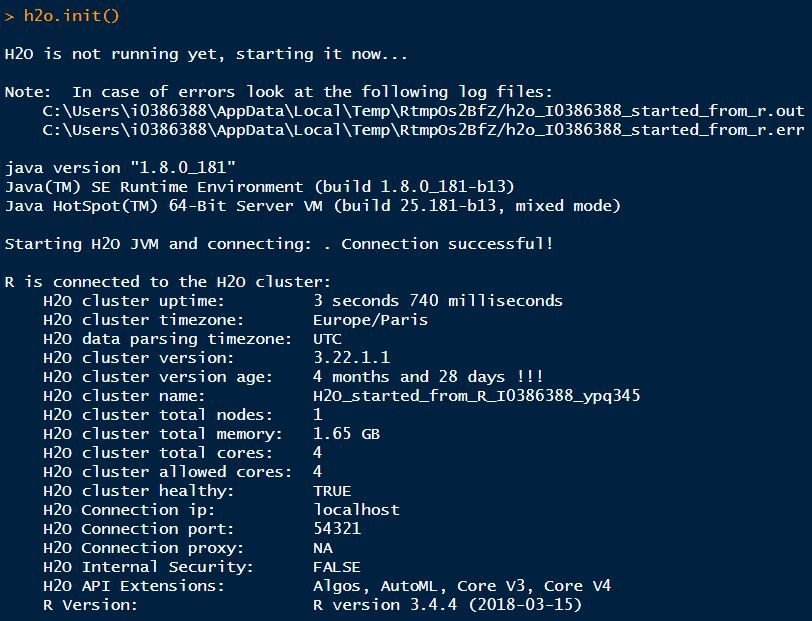
\includegraphics{h2o.png} \centering
\captionof{figure}{Información obtenida al inicializar el clúster h2o}

\setlength\parskip{5ex}
\justifying

\noindent Como se puede apreciar en la figura anterior, entre la
información que ofrece el paquete h2o ofrece inicializarse se encuentra
el mensaje al arrancar las máquinas virtuales Java sobre las que
trabaja, así como información relativa a la versión de los clústers que
se están utilizando, el nombre, número de nodos y núcleos que se procede
a utilizar, la memoria total y datos sobre la connectividad.

\noindent Para facilitar la aplicación de la función \texttt{AutoML} de
h2o se crea una función personalizada con 3 parámetros. Basta con
introducir la muestra de entramiento y la muestra de prueba, así como un
carácter con el nombre de la empresa (en este caso, combinación de
empresa + alisado + ventana de predicción). Esta función devuelve un
dataframe con las métricas AUC y \emph{accuracy} (con umbral de 0.5) ya
que son las métricas que se utilizan en el presente trabajo para evaluar
los modelos de clasificación binaria SMD. A su vez también se incluye la
etiqueta, o nombre, del modelo que mejor ha rendido sobre la muestra de
entrenamiento de entre todos los que la función \texttt{AutoML} prueba.
Esta función se puede encontrar en el anexo de esta testis, en el
apartado V.3.

\noindent Seguidamente se presentan los resultados para todas las
combinaciones de alisado y ventana de predicción sobre la empresa
Coca-Cola CO, ordenados de mayor a menor AUC.

\begin{table}[H]
\centering\begingroup\fontsize{10}{12}\selectfont

\begin{tabular}{l|r|r|l}
\hline
Company & AUC & Accuracy & Model\\
\hline
KO\_60\_2m & 0.9643794 & 0.6008677 & GBM\_4\_AutoML\_20190527\_133104\\
\hline
KO\_90\_1m & 0.9489899 & 0.7442827 & DRF\_1\_AutoML\_20190527\_133503\\
\hline
KO\_90\_2m & 0.9266426 & 0.7548807 & GLM\_grid\_1\_AutoML\_20190527\_133724\_model\_1\\
\hline
KO\_60\_3m & 0.9196836 & 0.7596372 & GLM\_grid\_1\_AutoML\_20190527\_133305\_model\_1\\
\hline
KO\_90\_3m & 0.9184683 & 0.6598639 & GLM\_grid\_1\_AutoML\_20190527\_133916\_model\_1\\
\hline
KO\_fun\_2m & 0.9123692 & 0.8546638 & DeepLearning\_1\_AutoML\_20190602\_194503\\
\hline
KO\_30\_3m & 0.8804991 & 0.5374150 & GBM\_5\_AutoML\_20190527\_132432\\
\hline
KO\_fun\_3m & 0.8796759 & 0.5736961 & GBM\_grid\_1\_AutoML\_20190602\_194733\_model\_1\\
\hline
KO\_60\_1m & 0.8794880 & 0.7879418 & GLM\_grid\_1\_AutoML\_20190527\_132816\_model\_1\\
\hline
KO\_30\_2m & 0.8525171 & 0.4295011 & GBM\_5\_AutoML\_20190527\_131607\\
\hline
KO\_fun\_1m & 0.7841235 & 0.4989605 & GLM\_grid\_1\_AutoML\_20190602\_194134\_model\_1\\
\hline
KO\_30\_1m & 0.6883664 & 0.5093555 & GLM\_grid\_1\_AutoML\_20190527\_125958\_model\_1\\
\hline
\end{tabular}
\endgroup{}
\end{table}
\centering
  \captionof{table}{Resultados modelo SMD aplicado a la empresa Coca-Cola KO utilizando automatic machine learning en h2o}

\setlength\parskip{5ex}
\justifying

\noindent En general el resultado de los modelos es bueno. Por lo que
respecta a la accuracy calculada con un umbral de 0.5 es en general
superior al 50\% de accuracy. A su vez, en obtienen unos AUC
relativamente elevados. El paquete h2o ha demostrado ser efectivo en
cuanto a la construcción de modelos con buen rendimiento. Todos menos un
modelo aplicados sobre los datos de la empresa Coca Cola obtienen un AUC
por encima de 0.85. En este caso el mayor AUC es de 0.96 y se obtiene
con un Gradient Boosting Machine sobre los datos de Coca Cola alisados
con una EMA a 60 días y prediciendo si el precio de cierre será más
elevado o más bajo a 2 meses vista. Seguidamente aparecen los modelos
sobre los datos alisados con EMA 90 días a 1 y 2 meses vista con AUC de
0.95 y 0.93 respectivamente. Los resultados obtenidos con el machine
learning automático son sorprendentemente buenos en relación al AUC
sobre muestra test. El hecho de que el rendimiento del modelo parezca
mejor usando el AUC en vez de la accuracy se debe a que la métrica
\textbf{accuracy} depende de un umbral predefinido (0.5), y posiblemente
el umbral óptimo para los modelos definidos no sea el de 0.5.

En cuanto a los distintos modelos escogidos cabe destacar que en 5 de
los 9 modelos escogidos para las 9 combinaciones de alisado y ventana de
predicción ha sido la regresión logística, etiquetada en este caso como
GLM\_grid

\noindent Finalmente se hace un ejercicio interesante, el de comparar la
\emph{accuracy} mostrada en la tabla anterior usando el paquete h2o con
la accuracy de los mismos modelos construidos en el apartado V.1. En
este caso los modelos son comparables al estar evaluados utilizando el
mismo periodo de prueba.

\begin{table}[H]
\centering\begingroup\fontsize{10}{12}\selectfont

\begin{tabular}{l|r|r|r|r|r|r}
\hline
Alisado & acc1m.h20 & acc1m & acc2m.h20 & acc2m & acc3m.h20 & acc3m\\
\hline
Alisado exponencial & 49.90 & 48.65 & 85.47 & 43.60 & 57.37 & 66.21\\
\hline
EMA30 & 50.94 & 41.16 & 42.95 & 45.12 & 53.74 & 57.82\\
\hline
EMA60 & 78.79 & 64.66 & 60.09 & 77.66 & 75.96 & 75.51\\
\hline
EMA90 & 74.43 & 84.41 & 75.49 & 65.08 & 65.99 & 69.84\\
\hline
\end{tabular}
\endgroup{}
\end{table}
\centering
  \captionof{table}{Comparativa de rendimiento obtenido con Random Forest con parámetros optimizados manualmente y los modelos construidos con ML automático H2O}

\setlength\parskip{5ex}
\justifying

\noindent Como se puede apreciar en la tabla anterior, los resultados de
accuracy calculada con un umbral de 0.5 son en general mejores
utilizando los modelos construidos automáticamente usando el paquete
H2O. Sin embargo sí que existen ciertas combinaciones para las cuales
los modelos Random Forest construidos, cuyos parámetros se optimizan
manualmente. No se aprecia ningún patrón claro que pueda distinguir para
que combinaciones es mejor qué modelo. Sin embargo, lo que sí se aprecia
es la diferencia que existe en cuanto a la carga de trabajo que supone
la construcción de ambos tipos de modelado. Mientras que la construcción
del modelo Random Forest requiere de un procedimiento de optimización de
parámetros manual, en el sentido que hay que escribir el proceso que
elabore el \emph{grid-search}, el proceso de modelado utilizando el ML
automático con el paquete H2O no requiere más que unas líneas de código
para elaborar el mismo tipo de optimización sobre muestra de validación,
previo al cálculo de las métricas sobre la muestra de entrenamiento.
Habiendo observado que los resultados son el general mejores, si más no
parecidos, utilizando ambos tipos de modelado, queda claro que el
\emph{trade-off} entre carga de trabajo y tiempo versus los resultados
lo gana el paquete H2O. Cabe destacar además que el hecho de construir
un modelo Gradient Boosting Machine y optimizarlo ``a mano'' es mucho
más laborioso que el de construir un Random Forest en cuanto a
complejidad del código, por lo que la opción de modelado con autoML de
H2O aparece muy atractiva a nivel usuario para según que tipo de
procesos de modelado. Por el contrario aparece como parte negativa el
carácter \emph{black-box} que tienen este tipo de sistemas automáticos
de machine learning, teniendo que confíar el usuario en los cálculos y
resultados que se ofrecen.

\FloatBarrier
\fancyhead[L]{Predicción de la rentabilidad: LSTM-RNN}
\fancyhead[R]{Sección V.4}
\fancyfoot[C]{\thepage}

\section{V.4 \textbf{Predicción del precio: LSTM-RNN}}

\noindent En el presente apartado se procede a construir una red
neuronal recurrente tipo LSTM para predecir los precios de cierre de la
empresa Coca Cola Co.. En hecho de escoger esta empresa está justificado
por distintas razones. En primer lugar el hecho de que solo sea una
empresa y no las 4 utilizadas como ejemplo en el apartado V.1 se debe a
que la capacidad computacional de la que se dispone es limitada. El
proceso de entrenamiento de un modelo de estas características requiere
de una elevada capacidad computacional para poder realizarse en un
periodo de tiempo relativamente razonable. En segundo lugar el hecho de
que sea Coca Cola y no una de las otras 3 empresas responde a lo
observado en el apartado V.1.1. Esta empresa es la que ofrece una opción
relativamente balanceada entre rentabilidad y riesgo. En tercer lugar la
tendencia creciente presente en parte de la serie parece ser
relativamente fuerte y la LSTM pueda probablemente captarlo.

\noindent Para emprezar se elabora el plan de entrenamiento del modelo
lstm. Con el procedimiento que se detalla a continuación permite obtener
una evaluación del rendimiento de este tipo de modelos en distintos
trozos de la serie temporal. En este caso se contruyen 6 submuestras que
conforman el plan de entrenamiento, cada una con 996 días en la muestra
de entrenamiento y 83 en la muestra de test. El por qué de esta
configuració se explica posteriormente en la parte de ajuste de los
parámetros. El tercer parámetro que define la partición del plan de
entrenamiento es el que controla la separación entre las ventanas
móviles. En este caso se define en 650 días. Esto significa que la
distancia entre el inicio de las series temporales en cada partición
está separado por 650 días. En definitiva el desarrollo que tiene este
apartado es el siguiente: por simplicidad, se procede a entrenar una
LSTM para cada partición creada, utilizando la misma combinación de
hyperparámetros para este modelo. En este apartado no se elabora una
optimización exhaustiva de los hyperparámetros de este modelo, que es de
hecho donde está la gran complejidad de los algoritmos de machine
learning, sino que se define una combinación de los mismos, que se
podría considerar como referencia para futuras optimizaciones. Esto es
así ya que en el momento de la elaboración de este trabajo no se dispone
de la capacidad computacional adecuada para poder elaborar una tarea de
semejante magnitud, al ser el periodo de tiempo considerado
relativamente elevado (18 años) y al ser el número de combinaciones de
hyper parámetros que hay que probar muy elevada. El hecho de entrenar
disintos modelos en distintos periodos de tiempo ofrece la posibilidad
de analizar el rendimiento de estos modelos con distintas predicciones a
lo largo del tiempo. El hecho de reducir el tamaño de la muestra de
entrenamiento para cada LSTM hace que el proceso de entrenamiento sea
mucho más rápido, con la contrapartida de que los modelos que se crean
no están ofreciendo todo su potencial.

\justifying

\noindent En la gráfica que se muestra a continuación se pueden ver
representadas las distintas particiones de la serie temporal de los
precios de cierre de Coca-Cola sobre los cuales se va a entrenar una
LSTM-RNN con el fin de testearla en los 83 días de muestra de prueba,
graficados en rojo.

\centering

\justifying

\begin{center}\includegraphics{figures/unnamed-chunk-90-1} \end{center}
\centering
  \captionof{figure}{Plan de entrenamiento de la LSTM para los precios de cierre. Fuente: elaboración propia}

\setlength\parskip{5ex}
\justifying

\noindent También se muestra el gráfico ampliado.

\begin{center}\includegraphics{figures/unnamed-chunk-91-1} \end{center}
\centering
  \captionof{figure}{Plan de entrenamiento de la LSTM para los precios de cierre. Ampliado. Fuente: elaboración propia}

\setlength\parskip{5ex}
\justifying

\noindent Una vez se tienen listas las particiones se procede a la
creación de los modelos LSTM sobre cada una de ellas. Cabe decir que la
implementación que se hace en este trabajo de los modelos LSTM se
soporta en el entorno Keras. En este caso se ha decidido utilizar la
implementación del entorno en keras en R, utilizando el paquete
\texttt{keras}, en vez de hacerlo en Python para mantener la integridad
de todo el trabajo en cuanto al software / lenguaje que se utiliza para
escribir y realizar los apartados de la presente tesis. Esta decisión
tiene implicaciones ya que el paquete \texttt{keras}, aunque trabaja
``por debajo'' con el entorno de programación TensorFlow, no permite
tener un control a tan bajo nivel de todos los hyper parámetros que se
pueden optimizar en un modelo de estas características.

\noindent Como se ha apuntado previamente, en el presente trabajo se
elaboran los modelos LSTM con una cierta combinación de parámetros,
debido a la alta capacidad computacional que requiere el hecho de hacer
el proceso de \emph{rolling origin cross validation} que este tipo de
modelos requieren para optimizar sus hyper parámteros. Los pasos en el
proceso de creación de estos modelos se detallan a continuación:

\begin{enumerate}
\def\labelenumi{\roman{enumi})}
\item
  En primer lugar se separan los datos de cada partición en sendas
  muestras de entrenamiento y prueba, teniendo la primera 996
  observaciones, es decir, días con valor en el precio de cierre de la
  empresa Coca Cola, mientras que la muestra de prueba consta de 83
  días. Esta separación entre muestras de entrenamiento y prueba
  responde al hecho que, a causa de la forma requerida del tensor de
  entrada en el modelo, el número de observaciones en la muestra de
  entrenamiento tiene que ser divisible entre el número de observaciones
  de la muestra de prueba, de manera que el resultado sea un número
  entero.
\item
  En segundo lugar se preprocesan los datos. En este caso se aplica en
  primer lugar la raíz cuadrada a los datos. Este proceso ayuda a
  reducir la varianza y eliminar los outliers. En segundo lugar se
  estandarizan los datos, restándoles la media y dividiéndolos por su
  desviación típica. Este proceso también se conoce como escalar y
  centrar los datos.
\item
  En tercer lugar se transforma la forma de los datos. Éstos necesitan
  ser transformados a forma de tensor, ya que es la forma requerida por
  este tipo de modelos. El concepto de tensor se puede pensar como una
  entidad algebraica que generaliza los conceptos de escalar, vector y
  matriz. Se podría entender como un vector de matrices, en este caso.
  En el presente trabajo la forma del tensor se detalla posteriormente
  en este apartado. Se construyen pues los tensores input y output de
  las muestras de entrenamiento y prueba.
\item
  En cuarto lugar se definen los hyper parámetros y se construye la
  función que se aplicará a cada partición para entrenar la LSTM. En
  cuanto a los parámetros, se presenta una restricción añadida a la
  descrita en el apartado i). El cociente entre el número de
  observaciones de la muestra de entrenamiento y el parámetro llamado
  \emph{batch size}, o tamaño del grupo, tiene que resultar también en
  un número entero. Esta regla también se aplica al número de
  observaciones en la muestra de prueba. El hyper parámetro \emph{batch
  size} controla el número de muestras, u observaciones, sobre las que
  se trabaja antes de actualizar los parámetros internos de la LSTM o
  pesos da la red. De hecho, es el número de observaciones que se
  utilizan para hacer las predicciones y así poder calcular el error que
  permite optimizar los pesos de la red. En el presente trabajo este
  parámetro se fija en 1 de manera que se está utilizando sólo 1
  observación a la vez para actualizar los parámetros internos del
  modelo. Esta configuración a la hora de utilizar el algoritmo de
  optimización del descenso del gradiente (Gradient Descent) para
  optimizar los pesos de la red se llama Stochastic Gradient Descent. Se
  sabe que fijar el \emph{batch size} en un valor pequeño aportan ruido
  y añaden un efecto regularizador que permite generalizar mejor.
  (Dominic Masters, 2018) presentan unos resultados en los que confirman
  que utilizando un valor pequeño para el parámetro \emph{batch size} se
  consigue obtener una estabilidad en el entrenamiento y una mejor
  generalización, dado una capacidad computacional, a través de un
  amplio abanico de experimentos.Otro de los parámetros que se fijan
  durante el entrenamiento de las LSTM es el número de épocas. Este
  hyper parámetro define el número de veces que el algoritmo va a
  aprender de todo el conjunto de datos. Es decir, terminar una época
  significa que cada muestra u observación en el conjunto de
  entrenamiento ha tenido la oportunidad de actualizar los parámetros
  internos del modelo o pesos de la red. Las épocas se fijan en 100 para
  limitar el tiempo de entrenamiento. También se fijan a 100 las
  unidades, o redes neuronales, internas de la LSTM. Este parámetro
  también se conoce como neuronas y controla la capacidad que tiene la
  LSTM de aprender. A más neuronas, más capacidad tiene la LSTM de
  aprender. Seguidamente se fija para el ajuste de la LSTM es el llamado
  \emph{time steps}. Este parámetro corresponde a la segunda dimensión
  del tensor de entrada. En este caso los tensores son de la forma
  \(Input = [996,1,1] , \ output=[83,1]\). Este hyper parámetro controla
  el número de observaciones en el pasado sobre las de las que la LSTM
  aprende. Como se ha detallado en el apartado IV.1 la LSTM es un tipo
  de red neuronal que permite aprender de periodos alejados en el
  tiempo, ya que es capaz de determinar la cantidad de información del
  pasado que hay que retener. Por añadidura, se fija el parámetro
  \emph{unit\_forget\_bias} a 1. Este hyper parámetro añade 1 al seso de
  la \emph{puerta de olvido} al inicializarse. Además añade una
  referencia a Jozefowicz et. al.~apuntando a que lo recomienda (Allaire
  \& Chollet, 2019). Finalmente cabe decir que la LSTM que se construye
  es de tipo \emph{STATEFULL}, tal y como se describe en el apartado
  IV.1.
\item
  En quinto lugar se entrena de manera iterativa sobre todas las épocas
  la LSTM.
\item
  Con el modelo entrenado, se calcula la predicción sobre la muestra de
  entrenamiento y se construye un \texttt{data\ frame} con los
  resultados reales y los predichos.
\end{enumerate}

\noindent Este proceso se aplica de manera iterativa sobre todas las
particiones y se grafican los resultados obtenidos sobre las muestras de
prueba. En rojo se pueden ver las predicciones, mientras que en negro se
dibujan los valores reales del precio de cierre.

\begin{center}\includegraphics{figures/unnamed-chunk-92-1} \end{center}
\centering
  \captionof{figure}{Resultados sobre muestra de prueba de la LSTM sobre los precios de cierre en particiones 1 y 2. Fuente: elaboración propia}

\setlength\parskip{5ex}
\justifying

\begin{center}\includegraphics{figures/unnamed-chunk-93-1} \end{center}
\centering
  \captionof{figure}{Resultados sobre muestra de prueba de la LSTM sobre los precios de cierre en particiones 3 y 4. Fuente: elaboración propia}

\setlength\parskip{5ex}
\justifying

\begin{center}\includegraphics{figures/unnamed-chunk-94-1} \end{center}
\centering
  \captionof{figure}{Resultados sobre muestra de prueba de la LSTM sobre los precios de cierre en particiones 5 y 6. Fuente: elaboración propia}

\setlength\parskip{5ex}
\justifying

\noindent Seguidamente se presenta la tabla que muestra el cálculo de
las distintas métricas de rendimiento para las distintas particiones:

\begin{verbatim}
##     Split     MAPE    MAPE2
## 1 split 1 1.992372 1.980983
## 2 split 2 7.150241 7.244746
## 3 split 3 6.203487 6.340186
## 4 split 4 2.233511 2.249743
## 5 split 5 1.820718 1.807583
## 6 split 6 3.279530 3.258063
\end{verbatim}

\noindent Como se puede observar en base al cálculo de los dos tipos de
MAPE, los resultados parecen bastante buenos. En la peor de las
particiones el modelo es capaz de generar un error percentual absoluto
medio de alrededor del 7\%. El MAPE2, modificado, muestra unos
resultados que son ligeramente mejores que la métrica del MAPE original,
pero aun así en general se observan buenos resultados. Aun habiendo
entrenado la LSTM sin optimizar los hyper parámetros y en el caso más
sencillo en el que los \emph{time steps} están fijados a 1 parece que se
obtiene un resultado relativamente bueno en términos de MAPE. Sin
embargo, una observación más detallada de las gráficas anteriores indica
que, aunque los valos predichos están en un nivel razonable, no son
capaces de captar los patrones que aparecen rápidamente, como podría ser
un crecimiento. Cabe destacar la predicción elaborada en la partición 2.
Los valores predichos tienen una tendencia decreciente, mientras que los
precios crecían. Esto se debe al gran decrecimiento que presentan los
datos en esta partición, en su primera mitad. El modelo LSTM entrenado
con esta partición aprende este partón y es el que intenta replicar al
hacer las predicciones.

\noindent Para facilitar la comparabilidad de las dos métricas se
presenta la siguiente visualización gráfica:

\includegraphics{figures/unnamed-chunk-97-1.pdf} \centering
\captionof{figure}{Métricas de rendimiento de las predicciones elaboradas con LSTM sobre las distintas particiones. Precio de cierre. Fuente: elaboración propia}

\setlength\parskip{5ex}
\justifying

\noindent Gracias a la figura anterior se puede ver fácilmente el punto
que se apuntaba previamente. La segunda métrica parece ofrecer
ligeramente unos valores inferiores pero en general los resultados
obtenidos en términos de MAPE son bastante postivios. Esto induce a
pensar que, disponiendo de una mayor capacidad computacional, este
modelo se podría mejorar más. La propuesta sería la de utilizar el
paquete \texttt{tfruns} para elaborar un \emph{grid search} sobre todas
las combinaciones de hyper parámetros disponibles. Esta técnica consiste
en probar todas las combinaciones de parámetros con tal de escoger la
combinación que ofrece un mejor resultado sobre la muestra de
validación. En este caso se hubiera propuesto una técnica de
cross-validación adaptada a las series temporales llamada \emph{rolling
origin cross-validation}, que permite mantener la estructura temporal de
la seria en el momento de hacer la optimización vía \emph{grid search}
en muestra de validación.

\noindent Seguidamente también se muestran dos métricas alternativas que
permiten evaluar la capacidad predictiva de los precios de la LSTM.
Éstas métricas son el Error Absoluto Medio (MAE) y el Cuadrado de la
Media de los errores al cuadrado (RMSE)

\begin{verbatim}
##   particiones       MAE      RMSE
## 1     split 1 0.4961335 0.6122746
## 2     split 5 0.7410633 0.8884039
## 3     split 4 0.7601204 1.3616478
## 4     split 6 1.3534583 1.6429215
## 5     split 3 1.4095112 1.7496488
## 6     split 2 1.6291732 1.9298185
\end{verbatim}

\noindent Como se puede apreciar en los resultados anteriores, ambas
métricas también muestran que en general se obtienen unos resultados
relativamente buenos. En ningún caso el RMSE pasa de 2 puntos en las
particiones, siendo la 1ª y la 5ª partición las que obtienen mejores
resultados, siendo su RMSE menor a 1. Sin embargo, las particiones que
obtienen peores resultados son las particiones 2 y 3.

\FloatBarrier
\fancyhead[L]{Predicción de la rentabilidad: LSTM-RNN}
\fancyhead[R]{Sección V.5}
\fancyfoot[C]{\thepage}

\section{V.5 \textbf{Predicción de la rentabilidad: LSTM-RNN}}

\noindent Una vez aplicada la LSTM sobre los precios de cierre
directamente, se explora la posibilidad de construir el mismo tipo de
modelos pero utilizando el logaritmo de las rentabilidades como serie
temporal. Los \emph{log returns} pueden verse desde una perspectiva
económica como la ganancia percentual entre dos precios, puediendo ser
su valor positivo o negativo. Desde un punto de vista estadístico lo que
busca esta transformación es que la serie temporal pase a ser
estacionaria de segundo orden al estar sus valores centrados en 0 y
tener (teóricamente) una varianza constante a lo largo del periodo
considerado. Sin embargo, este último punto no es del todo cierto en el
contexto del sector financiero ya que, al ser las series temporales
consideradas muy volátiles, no se consigue estabilizar totalmente la
varianza aplicando el logaritmo. Ésto se puede observar en los gráficos
que se muestran a continuación en los distintos picos que presenta la
rentabilidad, cosa que indica que la varianza no está del todo
estabilizada. Esta rentabilidad es la misma que se calcula en la sección
V.1 al hacer la descriptiva de las series temporales consideradas.

\justifying

\noindent La estrategia de entrenamiento de los modelos LSTM sobre la
rentabilidad es la misma que en el caso anterior sobre el precio. Se
elaboran 6 particiones y sus respectivas particiones sobre muestras de
entrenamiento y prueba. Los gráficos de las particiones se presentan a
continuación.

\begin{center}\includegraphics{figures/unnamed-chunk-103-1} \end{center}
\centering
  \captionof{figure}{Plan de entrenamiento de la LSTM para la rentabilidad de Coca Cola. Fuente: elaboración propia}

\setlength\parskip{5ex}
\justifying

\noindent Para facilitar la visualización se presentan también las
gráficas ampliadas:

\begin{center}\includegraphics{figures/unnamed-chunk-104-1} \end{center}
\centering
  \captionof{figure}{Plan de entrenamiento de la LSTM para los precios de cierre. Ampliado. Fuente: elaboración propia}

\setlength\parskip{5ex}
\justifying

\noindent La configuración de los hyper parámetros ha sido la misma que
en la sección V.4 donde se aplican los modelos LSTM sobre el precio. De
nuevo esto responde a un intento de simplificar la complejidad
computacional que presenta una optimización y entrenamiento intensivos
de estos modelos. A continuación se presentan graficados los valores
predichos en rojo encima de los valores reales en gris.

\begin{center}\includegraphics{figures/unnamed-chunk-105-1} \end{center}
\centering
  \captionof{figure}{Resultados sobre muestra de prueba de la LSTM sobre la rentabilidad en particiones 1 y 2. Fuente: elaboración propia}

\setlength\parskip{5ex}
\justifying

\begin{center}\includegraphics{figures/unnamed-chunk-106-1} \end{center}
\centering
  \captionof{figure}{Resultados sobre muestra de prueba de la LSTM sobre la rentabilidad en particiones 3 y 4. Fuente: elaboración propia}

\setlength\parskip{5ex}
\justifying

\begin{center}\includegraphics{figures/unnamed-chunk-107-1} \end{center}
\centering
  \captionof{figure}{Resultados sobre muestra de prueba de la LSTM sobre la rentabilidad en particiones 5 y 6. Fuente: elaboración propia}

\setlength\parskip{5ex}
\justifying

\noindent Para evaluar la capacidad predictiva de la LSTM que se acaba
de construir sobre la rentabilidad de la empresa Coca Cola se necesita
modificar ligeramente la métrica de MAPE presentada en M.4 ya que, al
ser la rentabilidad un estadístico que puede presentar valores tanto
negativos como positivos, hay que hacer el sumatorio del valor absoluto
del cociente, en vez de simplemente el valor absoluto del nominador.
Esto se debe al hecho de que los valores actuales, o reales, pueden ser
negativos. La nueva métrica de MAPE propuesta para el caso de la
rentabilidad es la siguiente:

\[MAPE_{bis} = \frac{1}{n}\sum_{i=1}^{n}\left | \frac{Actual_i \ -\ Predicted_i}{Actual_i}\right | \ \ \ \ \ \ \ \ \ \ \ \ \ \ (M.4bis)\]
\setlength\parskip{5ex}

\[MAPE_{2bis} = \frac{\sum_{i=1}^{n}\left |  Actual_i \ -\ Predicted_i\right |}{\sum_{i=1}^{n}\left |Actual_i \right |} \ \ \ \ \ \ \ \ \ \ \ \ \ \ (M.5bis)\]

\begin{verbatim}
##     Split      MAPE     MAPE2
## 1 split 1 105.68075 100.07356
## 2 split 2 100.00722  99.99388
## 3 split 3  99.92937  99.99064
## 4 split 4 100.00339 100.00138
## 5 split 5 100.00859 100.01386
## 6 split 6  99.35183  99.35015
\end{verbatim}

\noindent A continuación se presentan finalmente, siguiendo el formato
presentado en la sección V.4, las métricas de rendimiento sobre la
predicción que se acaba de generar para la rentabilidad de la empresa
Coca-Cola en las 6 particiones. En este caso las métricas que se
presentan finalmente para evaluar el rendimiento de las predicciones
hechas con la LSTM sobre la muestra de prueba de las rentabilidades son
el Error Medio Absoluto (MAE) y el RMSE.

\begin{verbatim}
##   particiones         MAE        RMSE
## 1     split 2 0.004537274 0.006794484
## 2     split 6 0.005404819 0.007326430
## 3     split 5 0.005718338 0.007525276
## 4     split 1 0.007031099 0.009317196
## 5     split 4 0.008861489 0.010917244
## 6     split 3 0.012347274 0.016499228
\end{verbatim}

\noindent Los resultados observados anteriormente llevan a pensar que
los modelos LSTM construidos con la rentabilidad sobre las distintas
particiones no son para nada unos modelos que ofrezcan buenos
resultados. Esto se puede ver a partir del cáluclo del MAPE, en
contrapartida a las métricas MAE y RMSE. El MAPE de todas las
particiones está sobre el 100\%. Esto significa que en porcentage, se
hace un 100\% de error respecto a los valores actuales. Cabe destacar
que para considerar un modelo predictivo como de alto rendimiento, el
MAPE debería ser inferior al 5\%. En este caso, los valores de la
rentabilidad son muy pequeños, del orden de 3 decimales, de manera que
una diferencia de 1 decimal implica un porcentage de error muy elevado.
Por ejemplo, si el valor actual de la rentabilidad es del 0.00019 y el
modelo predice un valor de 0.014 para el mismo periodo, uno se encuentra
con un error que es 6 veces mayor que el valor real. Es por esto que el
cálculo del MAPE ofrece valores tan elevados (alrededor del 100\%). Este
hecho se remarca ya que el cálculo del RMSE podría engañar al lector.
Aunque los cuadrados de los errores sean muy pequeños, esto no significa
que los modelos construidos sobre la rentabilidad tengan un buen
rendimiento (tal como indica el MAPE). Estos modelos presentan un RMSE
tan pequeño a causa del orden de los valores de la rentabilidad. Es
decir, al ser la rentabilidad un valor tan pequeño, del orden de 3 o 4
decimales, los cuadrados de los errores que se obtienen son, a su vez,
muy pequeños. Esto podría parecer la indicación de que los modelos
predictivos sobre la rentabilidad funcionan de una manera
sorprendentemente buena cuando, en realidad, no lo están haciendo, como
muestra el MAPE. En resumen: parece que los modelos LSTM construidos
sobre la rentabilidad no funcionan, ni de cerca, tan bien que los
modelos sobre el precio de cierre. El lector debe recordar que los
modelos LSTM se han construido con una configuración determinada al
disponer de una capacidad computacional limitada. Por ese motivo el
rendimiento de la LSTM sobre la rentabilidad se cree que puede mejorar
con una configuración optimizada de los hyper parámetros.

\FloatBarrier
\newpage
\fancyhead[L]{CONCLUSIONES}
\fancyhead[R]{\thechapter}
\fancyfoot[C]{}

\chapter{\textbf{CONCLUSIONES}}

\noindent Una vez terminadas las explicaciones de la parte práctica,
habiendo desarrollado todos los experimentos previamente, se procede a
la redacción de las conclusiones de la tesina. En primer lugar cabe
destacar que la exposición de las conclusiones se elabora en dos partes,
siguiendo la línea general del trabajo. Por un lado las conclusiones que
se extraen del análisis elaborado en el apartado III. Por el otro las
conclusiones extraídas de todos los experimentos que se elaboran en el
apartado V.4. La línea que se pretende seguir en la redacción de las
conclusiones es la siguiente. Para poder dar una visión general de todo
el trabajo, y de sus implicaciones, todas las conclusiones son extraídas
a partir de los objetivos fijados para este trabajo. En base a lo que se
pretendía analizar, se extraen las conclusiones en base a lo que se ha
elaborado.

\noindent Por lo que respecta al análisis de la situación actual de la
aplicación de la inteligencia artificial en el sector de las finanzas,
se han cubierto largamente las distintas aplicaciones que ésta tiene hoy
en día. Este análisis tenía por objetivo el obtener una visión global de
las distintas aplicaciones actuales con tal de poder analizar las
consecuencias que esta aplicación ha tenido. Las consecuencias
transversales que se han podido observar son las siguientes. En todas
las aplicaciones se aprecia la misma tónica y es que el aumento que está
experimentando en el siglo XXI la generación de datos, en cuanto a
volúmen, variedad y velocidad de generación permite la situación
perfecta para la proliferación de aplicaciones de IA que utilizan estos
grándes volúmenes de datos como fuente de información. Esto unido al
aumento de la capacidad computacional que conlleva la evolución
tecnológica ha permitido desarrollar aplicaciones nunca antes vistas,
que procesan este gran volumen de información, tradicional y nuevos
tipos de datos, de una manera muy rápida, y ha motivado la creación de
muchas empresas nuevas que se encargan de desarrollar nuevas soluciones
soportadas en sistemas de IA.

\noindent Desde una perspectiva de impacto positivo, se ha observado
que, de una manera transversal en las distintas aplicaciones analizadas,
una de las principales consecuencias de la existencia hoy en día de
sistemas de IA que reproducen más rápidamente las tareas que previamente
hacían los seres humanos es la reducción en los costes asociados. Esto
puede permitir en definitiva una mejora en la eficiencia general del
sector financiero. Otra de las consecuencias transversales que se
observa es la deriva que está tomando el sector financiero, por un
lado,hacia la aparición de nuevos agentes en el mismo que remueven a los
bancos de su posición oligopolística, y por otro, hacia la oferta de
servicios muchos más personalizados y adaptados a las necesidades
específicas de cada cliente. Paralelamente, se ha podido apreciar el
potencial que tiene la IA para contribuir al crecimiento económico,
visto desde una perspectiva macroeconómica.

\noindent Sin embargo, desde una perspectiva de impacto negativo se ha
observado una característica compartida por las distintas aplicaciones
analizadas. El caracter \emph{black-box} que suelen presentar este tipo
de modelos de \emph{machine learning}, en el sentido de que las
decisiones internas que toman no son comprensibles de una manera
sencilla, hace que todas los sistemas derivados de la utilización de
técnicas de IA y \emph{machine learning} tengan un carácter poco
transparente. El problema de la falta de transparencia a causa de la
utilización de estos modelos, que deriva del carácter poco comprensible
de los mismos, se presentará en un futuro como el mayor de los problemas
que van a tener que enfrentar las compañías, tanto privadas como
entidades reguladoras, que están utilizando o se plantean utilizar
sistemas de inteligencia artificial para complementar, mejorar o
sustituir sus actividades. En este sentido se aprecia también un
creciente interés por parte del sector público o regulatorio por la
aplicación de este tipo de sistemas, siguiendo como es habitual el
sector privado, que puede hacer cambiar en un futuro cómo se llevan a
cabo tareas tales como la detección de fraude. A raíz de esta falta de
transparencia presente en los actuales sistemas de IA en finanzas, se ha
podido apreciar una deriva creciente, tanto por parte de los
consumidores de servicios financieros basados en IA como de las mismas
compañías, hacia sistemas de IA que sean fácilmente explicables,
comprensibles y mucho más transparentes.

\noindent Otra de las potenciales consecuencias negativas que se observa
se deriva de la gran implantación que están teniendo este tipo de
servicios dentro del sector más clásico de los servicios financieros. La
presencia cada vez mayor de sistemas de IA totalmente automatizados
genera un potencial riesgo ya que puede contribuir a un efecto en cadena
de carácter extremadamente rápido si se produce en \emph{crash} en el
sector concreto en el que operen. Si muchos agentes confían en este tipo
de aplicaciones o modelos para llevar a cabo su actividad, los efectos
desencadenantes que esto puede tener frente a una situación de
\emph{shock} son extremadamente rápidos e incontrolables. Esto unido al
hecho de que los sistemas de IA en finanzas son mayoritariamente poco
transparentes puede dificultar en análisis a tiempo real de los sistemas
que están propagando un determinado \emph{crash}, e incluso puede
provocar que la comprensión de las causas de un determinado \emph{crash}
pueda extenderse durante semanas.

\noindent En general se observa que la situación actual de la
inteligencia artificial en el sector financiero es muy incierta.
Actualmente estamos viviendo una primera etapa de aplicación masiva,
donde muchos agentes empiezan a hacer el cambio hacia sistemas basados
íntegra o parcialmente en modelos de IA y \emph{machine learning}. La
previsión que se puede elaborar en base al análisis elaborado en esta
tesis es que la etapa de implantación aun puede durar entre 5 y 15 años,
de manera que la predicción a largo plazo es una entrada en una etapa de
madurez, donde la IA se usará en la gran mayoría de sub-sectores dentro
del sector financiero y habrá permitido mejorar, automatizar, crear y
destruir muchos de los empleos dentro de este sector que existen hoy en
día.

\noindent Por lo que respecta a las conclusiones que se extraen de los
experimentos realizados, se proceden a detallar las conclusiones
extraídas a partir de los distintos objetivos definidos. En primer lugar
el trabajo tenía por objetivo el definir un modelo de predicción de la
dirección de movimiento de un precio sobre 4 empresas concretas,
utilizando un modelo Random Forest con los parámetros optimizados.
Inicialmente se ha constatado que cada empresa presenta una serie
temporal de precios de cierre única, con patrones totalmente distintos y
con una alta volatilidad. Esto ha sido útil para poder tomar conciencia
de la dificultad de obtener rendimientos elevados de los modelos
predictivos aplicados a este tipo de datos. También se observa que el
hecho de alisar las series temporales reduce el ruido presente en los
datos y ayuda a predecir la dirección de movimiento del precio. Por lo
que respecta a la optimización de parámetros realizada se ha podido ver
que optimizar los parámetros sobre una muestra de validación que
consiste en un sólo año de datos, que además puede presentar un patrón
distinto a la muestra de prueba, provoca que los modelos generados con
dichos parámetros optimizados no tengan un buen rendimiento sobre
muestra de prueba. Esto se debe al hecho de que las series temporales
consideradas presentan numerosos cambios estructurales, que pueden tener
lugar entre la muestra de validación y la de prueba. En general, una vez
realizado el análisis se concluye que \emph{los indicadores técnicos
considerados en el presente trabajo son útiles cuando se trata de
predecir la dirección de movimiento del precio de cierre}. Aunque el
rendimiento obtenido de estos modelos no es el mismo para todas las
empresas, y en algunos casos no es útil para una situación real de
inversión, en general se observa que el hecho de añadir al modelo los
indicadores técnicos considerados mejora la predicción ingenua de 50\%
de probabilidad asignada a cada una de los dos niveles de la variable
respuesta (sube o baja).

\noindent En segundo lugar este trabajo tenía como objetivo el aplicar
este modelo conceptual de predicción de la dirección de movimiento de
una manera masiva, generalizada y utilizando computacion en paralelo,
sobre un gran conjunto de empresas. El interés de este objetivo es el de
poder aplicar este análisis en la realidad y así poder escoger la
empresa en la cual invertir en base al mejor rendimiento obtenido sobre
muestra de prueba. Pese a la limitada capacidad computacional de la que
se ha dispuesto durante la realización de la presente tesis se ha podido
realizar el análisis masivo paralelizando la computación para ganar
velocidad de cálculo. Gracias a esta aplicación general se ha podido
confirmar lo observado en el experimento con 4 empresas concretas. Los
indicadores técnicos aportan información útil que permite mejorar la
predicción ingenua a la hora de predecir la dirección de movimiento del
precio de cierre. Paralelamente se observa gracias a esta aplicación
generalizada que los modelos SMD parecen obtener generalmente mejores
resultados cuanto más cerca en el tiempo se hace la predicción. Es
decir, en general, se obtienen mejores rendimientos cuando se predice la
dirección que tomará el precio de cierre al cabo de un mes en vez de al
cabo de tres meses. Finalmente también se destaca que esta aplicación
masiva ha permitido confirmar una intuición que se desprende del ejemplo
concreto aplicado a 4 empresas: el rendimiento obtenido con este tipo de
modelos SMD depende de la empresa a la que se aplique, o lo que es lo
mismo, no todas las empresas obtienen un buen rendimiento usando este
tipo de modelos. De esto se deduce que parece existir algún tipo de
característica que hace que los modelos SMD aplicados a una determinada
empresa tengan mejor rendimiento que los aplicados en otra. Esta
investigación sobre esta característica podría ser el objeto de estudio
de posteriores tesis o artículos académicos.

\noindent En tercer lugar esta tesis pretendía indagar en el campo de
creciente implantación del \emph{machine learning} automatizado. Este
campo de estudio hace referencia a automatizar el proceso de creación de
modelos de ML tales como modelos tipo \emph{ensemble}, de manera que el
usuario no tenga que construirlos ``a mano''. Gracias a la aplicación de
los modelos SMD construidos de una manera automática usando todos los
modelos disponibles en el paquete de R \emph{h2o} se ha podido comprobar
que se obtiene un rendimiento generalmente parecido al obtenido
utilizando los modelos Random Forest. Sin embargo, la conclusión a la
que se llega es que, en realidad, la utilización de funciones
automatizadas para la creación de modelos de ML parece generalmente más
interesante ya que permite obtener más o menos el mismo rendimiento que
los modelos Random Forest creados manualmente pero con un esfuerzo o
carga de trabajo muy inferiores. Resultados generalmente parecidos con
muchas menos horas de trabajo en su realización. Este hecho ha permitido
tomar conciencia de que la automatización en la construcción de modelos
de ML es una de las tendencias que tiene mayor fuerza en el desarrollo
teórico actual del campo de la inteligencia artificial. El hecho de
automatizar una tarea, como puede ser la construcción de modelos de IA,
puede permitir a la humanidad seguir desarrollando ideas en este campo,
de manera que su continua evolución parece estar garantizada.

\noindent En cuarto lugar, otro de los grandes objetivos del presente
trabajo era el de estudiar, en paralelo a la aplicación de los modelos
SMD, la construcción de modelos predictivos entrenados directamente
sobre el precio de cierre y la rentabilidad. En este sentido, también se
pretendía analizar el rendimiento que pueden ofrecer los modelos
llamados LSTM, al ser éstos capaces de recordar dependencias temporales
grandes. Este tipo de modelos están en auge hoy en día a causa de su
gran rendimiento en un variado abanico de aplicaciones, y es por eso que
se consideraron ideales para ser probados sobre los datos concretos de
una empresa. Aunque los precios de cierre son difíciles de predecir con
modelos estadísticos clásicos, el tipo de redes neuronales recurrentes
LSTM que se han utilizado en el presente trabajo han probado ser, tras
su aplicación satisfactoria, capaces de captar relaciones que no son
capaces de captar los modelos estadísticos clásicos. Sin embargo este
tipo de modelos se ha aplicado sobre una empresa concreta por
simplicidad, por lo que el rendimiento sobre otras empresas es por el
momento inexplorado. A su vez, también se constata que sólo se ha
realizado el primer paso de todo un seguido de procedimientos que
deberían realizarse para aumentar la capacidad predictiva de estos
modelos. Durante la redacción de esta tesis no se ha podido disponer de
una alta elevada capcidad computacional por lo que se han tenido que
mantener estáticos los hyper-parámetros de estos modelos. Por esta
razón, se llega a la conclusión de que aun existe un gran potencial
latente en este tipo de modelos en cuanto al rendimiento predictivo, que
sólo se puede obtener disponiendo de una gran capacidad computacional.
Este aumento en la capacidad predictiva vendrá dado por una optimización
intensiva de los hyper parámetros del modelo y por un proceso de
entrenamiento suficientemente extenso, y ésto sólo se puede conseguir
disponiendo de una alta capacidad computacional. De no ser así, el
usuario intentando optimizar y entrenar este tipo de modelos se verá a
si mismo enfrentando una gran cantidad de horas de espera requeridas
hasta la finalización de dicho proceso de optimización y entrenamiento.

\FloatBarrier
\newpage
\fancyhead[L]{BIBLIOGRAFÍA}
\fancyhead[R]{\thepage}
\fancyfoot[C]{}

\chapter{\textbf{\hspace{1pt} BIBLIOGRAFÍA}}

\setlength{\parindent}{-0.5in}
\setlength{\leftskip}{0.4in}
\setlength{\parskip}{6pt}

\noindent

\hypertarget{refs}{}
\leavevmode\hypertarget{ref-keras}{}%
Allaire, J., \& Chollet, F. (2019). \emph{Keras: R interface to
'keras'}. Retrieved from \url{https://CRAN.R-project.org/package=keras}

\leavevmode\hypertarget{ref-crisisreasons}{}%
Andrew K. Rose, M. M. S. (2011). Cross-country causes and consequences
of the 2008 crisis: Early warning. \emph{Japan and the World Economy}.

\leavevmode\hypertarget{ref-Chen}{}%
An-Sing Chena, H. D., Mark T. Leungb. (2003). Application of neural
networks to an emerging financial market: Forecasting and trading the
taiwan stock index. \emph{Computers \& Operations Research, 30 (6)
(2003)}, 901--923. Retrieved from
\url{https://ac.els-cdn.com/S0305054802000370/1-s2.0-S0305054802000370-main.pdf?_tid=a9ff1500-f141-436c-9298f0bf19d9c5c0\&acdnat=1545913123_1b0ff6cdd7d647a8c5e9891ad3f6ea65}

\leavevmode\hypertarget{ref-AIboard}{}%
Board, F. S. (2017). \emph{Artificial intelligence and machine learning
in financial services. Market developments and financial stability
implications}. 4--34.

\leavevmode\hypertarget{ref-protrader}{}%
Chen, L. (1989). \emph{Protrader: An expert system for strock trading}.

\leavevmode\hypertarget{ref-Huang}{}%
C.L. Huang, C. T. (2009). A hybrid sofm-svr with a filter-based feature
selection for stock market forecasting. \emph{Expert Systems with
Applications, 36 (2) (2009)}, 1529--1539. Retrieved from
\url{https://ac.els-cdn.com/S0957417407006069/1-s2.0-S0957417407006069-main.pdf?_tid=ffd2e07d-4100-4d76bc64-653d8ae68de7\&acdnat=1545913369_ce2c3b4a4eb42518498e95713c23e5c3}

\leavevmode\hypertarget{ref-marketimpact}{}%
Day, S. (2017). \emph{Quants turn to machine learning to model market
impact}. RISK Magazine.

\leavevmode\hypertarget{ref-crisisreasons2}{}%
DeLong, J. B. (2009). The financial crisis of 2007--2009: Understanding
its causes, consequences---and its possible cures. \emph{MTI-CSC
Economics Speaker Series Lecture}.

\leavevmode\hypertarget{ref-ensemble}{}%
Dietterich, T. G. (n.d.). \emph{Ensemble methods in machine learning}.
Retrieved from
\url{http://citeseerx.ist.psu.edu/viewdoc/download?doi=10.1.1.34.4718rep=rep1type=pdf}

\leavevmode\hypertarget{ref-smallbatch}{}%
Dominic Masters, C. L. (2018). \emph{Revisiting small batch training for
deep neural networks}.

\leavevmode\hypertarget{ref-KPMG}{}%
Funcas, K. y. (2017). \emph{Fintech: Innovación al servicio del
cliente}. 7.

\leavevmode\hypertarget{ref-CoVMike}{}%
Gilliland, M. (2009). The coefficient of variation for assessing
forecastability. \emph{The Business Forecasting Deal}.

\leavevmode\hypertarget{ref-FinCENblanqueo}{}%
Golberg, e. a. (1995). \emph{The fincen artificial intelligence systems:
Identifying potential money laundering from reports of large cash
transactions}.

\leavevmode\hypertarget{ref-zichao}{}%
Han, Z. (2012). \emph{Data and text mining of financial markets using
news and social media}. 1--102. Retrieved from
\url{https://studentnet.cs.manchester.ac.uk/resources/library/thesis_abstracts/MSc12/FullText/Han-Zhichao-fulltext.pdf}

\leavevmode\hypertarget{ref-HFTbank}{}%
Jonathan Brogaard, T. H., \& Riordan, R. (2013). High frequency trading
and price discovery. \emph{Working Paper Series}, 2--57.

\leavevmode\hypertarget{ref-machinelearning}{}%
Jordan, M., \& Mitchell, T. (2015). \emph{Machine learning: Trends,
perspectives, and prospects}.

\leavevmode\hypertarget{ref-kim2003}{}%
Kim, K.-j. (2003). Financial time series forecasting using support
vector machines. \emph{Neurocomputing 55 (2003)}, 307--319. Retrieved
from
\url{https://ac.els-cdn.com/S0925231203003722/1-s2.0-S0925231203003722-main.pdf?_tid=ec7d432b-e65c-434eb695-6d2035ff9829\&acdnat=1545911976_ef14d01ea7992160caa0d8b4aa7c13aa}

\leavevmode\hypertarget{ref-black}{}%
Knight, W. (2017). \emph{The dark secret at the heart of ai}.

\leavevmode\hypertarget{ref-privacy}{}%
Kuroda, H. (2016). \emph{Information technology and financial services:
The central bank's perspective}.

\leavevmode\hypertarget{ref-comodities}{}%
Lambert, D. (1980). \emph{Commodities(now called futures)}.

\leavevmode\hypertarget{ref-expertsystems}{}%
Leondes, C. T. (2002). \emph{Expert systems: The technology of knowledge
management and decision making for the 21st century} (pp. 1--22).

\leavevmode\hypertarget{ref-RF}{}%
Liaw, A., \& Wiener, M. (2002). Classification and regression by
randomForest. \emph{R News}, \emph{2}(3), 18--22. Retrieved from
\url{https://www.r-project.org/doc/Rnews/Rnews_2002-3.pdf}

\leavevmode\hypertarget{ref-saha2016}{}%
Luckyson Khaidem, S. R. D., Snehanshu Saha. (2016). Predicting the
direction of stock market prices using random forest. \emph{To Appear in
Applied Mathematical Finance}, 21.

\leavevmode\hypertarget{ref-ManishKumar}{}%
Manish Kumar, M. T. (2006). Forecasting stock index movement: A
comparison of support vector machines and random forest. \emph{Indian
Institute of Capital Markets 9th Capital Markets Conference Paper}.
Retrieved from
\url{https://papers.ssrn.com/sol3/papers.cfm?abstract_id=876544}

\leavevmode\hypertarget{ref-najeb}{}%
Masoud, N. (2014). Predicting direction of stock prices indexmovement
using artificial neural networks:The case of libyan financial market.
\emph{British Journal of Economics, Management \& Trade}, 597--619.

\leavevmode\hypertarget{ref-pamelamachines}{}%
McCorduck, P. (2004). \emph{Machines who think (2nd ed.)}. A. K. Peters,
Ltd.

\leavevmode\hypertarget{ref-modeldef}{}%
Mitchell, C. (2016). \emph{Model validation: For elements of determining
the accuracy of your model}. British Bankers Association.

\leavevmode\hypertarget{ref-LSTMteoria}{}%
Olah, C. (2015). \emph{Understanding lstm networks}. Retrieved from
\url{http://colah.github.io/posts/2015-08-Understanding-LSTMs/}

\leavevmode\hypertarget{ref-HFT}{}%
Oliver Linton, S. M. (2018). Implications of high-frequency trading for
security markets. \emph{Cemmap}, 1--24.

\leavevmode\hypertarget{ref-biascredit}{}%
O'Neil, C. (2016). \emph{Weapons of math destruction: How big data
increases inequality and threatens democracy}. London: Allen Lane.

\leavevmode\hypertarget{ref-tuningRF}{}%
Philipp Probst, M. W., \& Boulesteix, A.-L. (2018).
\emph{Hyperparameters and tuning strategies for random forest}.
Retrieved from \url{https://arxiv.org/pdf/1804.03515.pdf}

\leavevmode\hypertarget{ref-crisisreasons3}{}%
P.R. Lane, G. M.-F. (2011). The cross-country incidence of the global
crisis. \emph{IMF Economic Review}, \emph{59}, 77--110.

\leavevmode\hypertarget{ref-Tsaih1998}{}%
Ray Tsaih, C. C. L., Yenshan Hsu. (1998). Forecasting s\&P 500 stock
index futures with a hybrid ai system. \emph{Decision Support Systems,
23 (1998)}, 161--174. Retrieved from
\url{https://ac.els-cdn.com/S0167923698000281/1-s2.0-S0167923698000281-main.pdf_tid=5c0465f0-1321-4ffd-920b-4ff50ab6fd3b\&acdnat=1545912698_86722ea4bbc2cf26a7590b8bdfeab92d}

\leavevmode\hypertarget{ref-IOSCO}{}%
Securities Commissions, I. O. of. (2017). \emph{Research report on
financial technologies (fintech)}.

\leavevmode\hypertarget{ref-creditscoring1}{}%
Stefan Lessmann, H.-V. S., Bart Baesens, \& Thomas, L. (2015).
Benchmarking state-of-the art classification algorithms for credit
scoring: An update of research. In \emph{European Journal of Operational
Research 247} (pp. 124--136).

\leavevmode\hypertarget{ref-aimodern}{}%
Stuart Russel, P. N. (1995). Artificial intelligence. Modern approach.
\emph{New Jersey: Prentice Hall, Englewood Cliffs}.

\leavevmode\hypertarget{ref-TTR}{}%
Ulrich, J. (2018). \emph{TTR: Technical trading rules}. Retrieved from
\url{https://CRAN.R-project.org/package=TTR}

\leavevmode\hypertarget{ref-stockboomJermann}{}%
Urban Jermann, V. Q. (2003). \emph{Stock market boom and the
productivity gains of the 1990s}.

\leavevmode\hypertarget{ref-warrenbuffet}{}%
\emph{Warren buffett : Latest portfolio}. (n.d.).
\url{http://warrenbuffettstockportfolio.com/}.

\leavevmode\hypertarget{ref-ATR}{}%
Wilder, J. (1978). New concepts in technical trading systems.
\emph{Trend Research Greensboro, North Carolina}.

\leavevmode\hypertarget{ref-macro}{}%
Wilkins, C. (2017). \emph{Blame it on the machines?}

\leavevmode\hypertarget{ref-Dartmouth_workshop}{}%
workshop, W. D. (2019). \emph{Dartmouth workshop --- Wikipedia, the free
encyclopedia}.
\url{http://en.wikipedia.org/w/index.php?title=Dartmouth\%20workshop\&oldid=878151960}.

\leavevmode\hypertarget{ref-yakupkara}{}%
Yakup Kara, Ö. K. B., Melek Acar Boyacioglu. (2011). Predicting
direction of stock price index movement using artificial neural networks
and support vector machines: The sample of the istanbul stock exchange.
\emph{Expert Systems with Applications}, 5311--5319. Retrieved from
\href{https://ac.els-cdn.com/S0957417410011711/1-s2.0-S0957417410011711-main.pdf?_tid=e5e12593-4a56-4db0-9d5f\%20ff9784196726\&acdnat=1545074291_d05308f34977383caaff6ae009a6acf5}{https://ac.els-cdn.com/S0957417410011711/1-s2.0-S0957417410011711-main.pdf?\_tid=e5e12593-4a56-4db0-9d5f ff9784196726\&acdnat=1545074291\_d05308f34977383caaff6ae009a6acf5}

\leavevmode\hypertarget{ref-Huang2}{}%
Y. Nakamori, S. W., W. Huang. (2005). Forecasting stock market movement
direction with support vector machine. \emph{Computers \& Operations
Research, 32 (10)}, 2513--2522.

\FloatBarrier
\newpage
\fancyhead[L]{ANEXO}
\fancyhead[R]{Capítulo \thechapter}
\fancyfoot[C]{\thepage}

\chapter{\textbf{\hspace{1pt} ANEXO}}
\setlength{\parindent}{1cm}
\setlength{\leftskip}{0.0in}

En el siguiente anexo se añaden los scripts utilizados en el presente
trabajo, ordenados por secciones siguiendo la estructura del mismo.
Teniendo en cuenta que la propia tesis se ha escrito en R Markdown
utilizando LaTeX como soporte, cabe destacar el hecho de que en el anexo
se incluyen sólo los códigos para generar las partes técnicas del mismo,
no el codigo de R Markdown para generar la tesis. Éste se puede
encontrar en un proyecto en el siguiente enlace de GitHub:
\url{https://github.com/ArnauMunsOrenga/TFG}. Sin embargo, sí que se
incluye el código necesario para generar las tablas y los gráficos.

\emph{Apartado V.1}

\setlength\parskip{5ex}

\hypertarget{obtencion-y-descripcion}{%
\paragraph{Obtención y descripción}\label{obtencion-y-descripcion}}

\scriptsize

\begin{Shaded}
\begin{Highlighting}[]
\KeywordTok{library}\NormalTok{(CombMSC)}
\KeywordTok{library}\NormalTok{(randomForest)}
\KeywordTok{library}\NormalTok{(quantmod)}
\KeywordTok{library}\NormalTok{(TTR)}
\KeywordTok{library}\NormalTok{(tidyverse)}
\KeywordTok{library}\NormalTok{(caret)}
\KeywordTok{library}\NormalTok{(foreach)}
\KeywordTok{library}\NormalTok{(kableExtra)}
\KeywordTok{library}\NormalTok{(dplyr)}
\KeywordTok{library}\NormalTok{(formatR)}

\KeywordTok{getSymbols}\NormalTok{(}\DataTypeTok{Symbols =} \StringTok{"KO"}\NormalTok{, }\DataTypeTok{from =} \StringTok{"2000-01-01"}\NormalTok{, }\DataTypeTok{to =} \StringTok{"2018-12-31"}\NormalTok{)}
\KeywordTok{getSymbols}\NormalTok{(}\DataTypeTok{Symbols =} \StringTok{"WFC"}\NormalTok{, }\DataTypeTok{from =} \StringTok{"2000-01-01"}\NormalTok{, }\DataTypeTok{to =} \StringTok{"2018-12-31"}\NormalTok{)}
\KeywordTok{getSymbols}\NormalTok{(}\DataTypeTok{Symbols =} \StringTok{"AAPL"}\NormalTok{, }\DataTypeTok{from =} \StringTok{"2000-01-01"}\NormalTok{, }\DataTypeTok{to =} \StringTok{"2018-12-31"}\NormalTok{)}
\KeywordTok{getSymbols}\NormalTok{(}\DataTypeTok{Symbols =} \StringTok{"AXP"}\NormalTok{, }\DataTypeTok{from =} \StringTok{"2000-01-01"}\NormalTok{, }\DataTypeTok{to =} \StringTok{"2018-12-31"}\NormalTok{)}

\NormalTok{prices.KO <-}\StringTok{ }\KeywordTok{as.data.frame}\NormalTok{(KO)}
\NormalTok{prices.WFC <-}\StringTok{ }\KeywordTok{as.data.frame}\NormalTok{(WFC)}
\NormalTok{prices.AAPL <-}\StringTok{ }\KeywordTok{as.data.frame}\NormalTok{(AAPL)}
\NormalTok{prices.AXP <-}\StringTok{ }\KeywordTok{as.data.frame}\NormalTok{(AXP)}
\KeywordTok{str}\NormalTok{(prices.KO)}


\NormalTok{a <-}\StringTok{ }\KeywordTok{format}\NormalTok{(}\KeywordTok{data.frame}\NormalTok{(}\KeywordTok{paste0}\NormalTok{(}\KeywordTok{round}\NormalTok{(}\KeywordTok{summary}\NormalTok{(prices.KO}\OperatorTok{$}\NormalTok{KO.Open), }
    \DecValTok{2}\NormalTok{)) }\OperatorTok\StringTok{ }\KeywordTok{rbind}\NormalTok{(}\DataTypeTok{a =} \KeywordTok{paste0}\NormalTok{(}\KeywordTok{round}\NormalTok{(}\KeywordTok{summary}\NormalTok{(prices.KO}\OperatorTok{$}\NormalTok{KO.High), }
    \DecValTok{2}\NormalTok{))) }\OperatorTok\StringTok{ }\KeywordTok{rbind}\NormalTok{(}\DataTypeTok{b =} \KeywordTok{paste0}\NormalTok{(}\KeywordTok{round}\NormalTok{(}\KeywordTok{summary}\NormalTok{(prices.KO}\OperatorTok{$}\NormalTok{KO.Low), }
    \DecValTok{2}\NormalTok{))) }\OperatorTok\StringTok{ }\KeywordTok{rbind}\NormalTok{(}\DataTypeTok{c =} \KeywordTok{paste0}\NormalTok{(}\KeywordTok{round}\NormalTok{(}\KeywordTok{summary}\NormalTok{(prices.KO}\OperatorTok{$}\NormalTok{KO.Close), }
    \DecValTok{2}\NormalTok{))) }\OperatorTok\StringTok{ }\KeywordTok{rbind}\NormalTok{(}\KeywordTok{paste0}\NormalTok{(}\KeywordTok{round}\NormalTok{(}\KeywordTok{summary}\NormalTok{(prices.KO}\OperatorTok{$}\NormalTok{KO.Volume)}\OperatorTok{/}\FloatTok{1e+06}\NormalTok{, }
    \DecValTok{3}\NormalTok{), }\StringTok{"M"}\NormalTok{))), }\DataTypeTok{scientific =} \OtherTok{TRUE}\NormalTok{)}

\KeywordTok{rownames}\NormalTok{(a) <-}\StringTok{ }\KeywordTok{c}\NormalTok{(}\StringTok{"Open"}\NormalTok{, }\StringTok{"High"}\NormalTok{, }\StringTok{"Low"}\NormalTok{, }\StringTok{"Close"}\NormalTok{, }\StringTok{"Volume"}\NormalTok{)}
\KeywordTok{names}\NormalTok{(a) <-}\StringTok{ }\KeywordTok{names}\NormalTok{(}\KeywordTok{summary}\NormalTok{(prices.KO}\OperatorTok{$}\NormalTok{KO.Open))}

\KeywordTok{kable}\NormalTok{(a, }\StringTok{"latex"}\NormalTok{, }\DataTypeTok{digits =} \DecValTok{2}\NormalTok{) }\OperatorTok\StringTok{ }\KeywordTok{kable_styling}\NormalTok{(}\DataTypeTok{font_size =} \DecValTok{10}\NormalTok{, }
    \DataTypeTok{latex_options =} \KeywordTok{c}\NormalTok{(}\StringTok{"basic"}\NormalTok{))}
\CommentTok{# \{Estadísticos descriptivos para los distintos precios de}
\CommentTok{# Coca-Cola Company\}}


\NormalTok{a <-}\StringTok{ }\KeywordTok{format}\NormalTok{(}\KeywordTok{data.frame}\NormalTok{(}\KeywordTok{paste0}\NormalTok{(}\KeywordTok{round}\NormalTok{(}\KeywordTok{summary}\NormalTok{(prices.AAPL}\OperatorTok{$}\NormalTok{AAPL.Open), }
    \DecValTok{2}\NormalTok{)) }\OperatorTok\StringTok{ }\KeywordTok{rbind}\NormalTok{(}\DataTypeTok{a =} \KeywordTok{paste0}\NormalTok{(}\KeywordTok{round}\NormalTok{(}\KeywordTok{summary}\NormalTok{(prices.AAPL}\OperatorTok{$}\NormalTok{AAPL.High), }
    \DecValTok{2}\NormalTok{))) }\OperatorTok\StringTok{ }\KeywordTok{rbind}\NormalTok{(}\DataTypeTok{b =} \KeywordTok{paste0}\NormalTok{(}\KeywordTok{round}\NormalTok{(}\KeywordTok{summary}\NormalTok{(prices.AAPL}\OperatorTok{$}\NormalTok{AAPL.Low), }
    \DecValTok{2}\NormalTok{))) }\OperatorTok\StringTok{ }\KeywordTok{rbind}\NormalTok{(}\DataTypeTok{c =} \KeywordTok{paste0}\NormalTok{(}\KeywordTok{round}\NormalTok{(}\KeywordTok{summary}\NormalTok{(prices.AAPL}\OperatorTok{$}\NormalTok{AAPL.Close), }
    \DecValTok{2}\NormalTok{))) }\OperatorTok\StringTok{ }\KeywordTok{rbind}\NormalTok{(}\KeywordTok{paste0}\NormalTok{(}\KeywordTok{round}\NormalTok{(}\KeywordTok{summary}\NormalTok{(prices.AAPL}\OperatorTok{$}\NormalTok{AAPL.Volume)}\OperatorTok{/}\FloatTok{1e+06}\NormalTok{, }
    \DecValTok{3}\NormalTok{), }\StringTok{"M"}\NormalTok{))), }\DataTypeTok{scientific =} \OtherTok{TRUE}\NormalTok{)}

\KeywordTok{rownames}\NormalTok{(a) <-}\StringTok{ }\KeywordTok{c}\NormalTok{(}\StringTok{"Open"}\NormalTok{, }\StringTok{"High"}\NormalTok{, }\StringTok{"Low"}\NormalTok{, }\StringTok{"Close"}\NormalTok{, }\StringTok{"Volume"}\NormalTok{)}
\KeywordTok{names}\NormalTok{(a) <-}\StringTok{ }\KeywordTok{names}\NormalTok{(}\KeywordTok{summary}\NormalTok{(prices.KO}\OperatorTok{$}\NormalTok{KO.Open))}
\KeywordTok{kable}\NormalTok{(a, }\StringTok{"latex"}\NormalTok{) }\OperatorTok\StringTok{ }\KeywordTok{kable_styling}\NormalTok{(}\DataTypeTok{font_size =} \DecValTok{10}\NormalTok{, }\DataTypeTok{latex_options =} \KeywordTok{c}\NormalTok{(}\StringTok{"basic"}\NormalTok{))}

\CommentTok{# \{Estadísticos descriptivos para los distintos precios de}
\CommentTok{# Apple Inc.\}}


\NormalTok{a <-}\StringTok{ }\KeywordTok{format}\NormalTok{(}\KeywordTok{data.frame}\NormalTok{(}\KeywordTok{paste0}\NormalTok{(}\KeywordTok{round}\NormalTok{(}\KeywordTok{summary}\NormalTok{(prices.AXP}\OperatorTok{$}\NormalTok{AXP.Open), }
    \DecValTok{2}\NormalTok{)) }\OperatorTok\StringTok{ }\KeywordTok{rbind}\NormalTok{(}\DataTypeTok{a =} \KeywordTok{paste0}\NormalTok{(}\KeywordTok{round}\NormalTok{(}\KeywordTok{summary}\NormalTok{(prices.AXP}\OperatorTok{$}\NormalTok{AXP.High), }
    \DecValTok{2}\NormalTok{))) }\OperatorTok\StringTok{ }\KeywordTok{rbind}\NormalTok{(}\DataTypeTok{b =} \KeywordTok{paste0}\NormalTok{(}\KeywordTok{round}\NormalTok{(}\KeywordTok{summary}\NormalTok{(prices.AXP}\OperatorTok{$}\NormalTok{AXP.Low), }
    \DecValTok{2}\NormalTok{))) }\OperatorTok\StringTok{ }\KeywordTok{rbind}\NormalTok{(}\DataTypeTok{c =} \KeywordTok{paste0}\NormalTok{(}\KeywordTok{round}\NormalTok{(}\KeywordTok{summary}\NormalTok{(prices.AXP}\OperatorTok{$}\NormalTok{AXP.Close), }
    \DecValTok{2}\NormalTok{))) }\OperatorTok\StringTok{ }\KeywordTok{rbind}\NormalTok{(}\KeywordTok{paste0}\NormalTok{(}\KeywordTok{round}\NormalTok{(}\KeywordTok{summary}\NormalTok{(prices.AXP}\OperatorTok{$}\NormalTok{AXP.Volume)}\OperatorTok{/}\FloatTok{1e+06}\NormalTok{, }
    \DecValTok{3}\NormalTok{), }\StringTok{"M"}\NormalTok{))), }\DataTypeTok{scientific =} \OtherTok{TRUE}\NormalTok{)}

\KeywordTok{rownames}\NormalTok{(a) <-}\StringTok{ }\KeywordTok{c}\NormalTok{(}\StringTok{"Open"}\NormalTok{, }\StringTok{"High"}\NormalTok{, }\StringTok{"Low"}\NormalTok{, }\StringTok{"Close"}\NormalTok{, }\StringTok{"Volume"}\NormalTok{)}
\KeywordTok{names}\NormalTok{(a) <-}\StringTok{ }\KeywordTok{names}\NormalTok{(}\KeywordTok{summary}\NormalTok{(prices.KO}\OperatorTok{$}\NormalTok{KO.Open))}
\KeywordTok{kable}\NormalTok{(a, }\StringTok{"latex"}\NormalTok{, }\DataTypeTok{digits =} \DecValTok{2}\NormalTok{) }\OperatorTok\StringTok{ }\KeywordTok{kable_styling}\NormalTok{(}\DataTypeTok{font_size =} \DecValTok{10}\NormalTok{, }
    \DataTypeTok{latex_options =} \KeywordTok{c}\NormalTok{(}\StringTok{"basic"}\NormalTok{))}
\CommentTok{# \{Estadísticos descriptivos para los distintos precios de}
\CommentTok{# American Express CO.\}}


\NormalTok{a <-}\StringTok{ }\KeywordTok{format}\NormalTok{(}\KeywordTok{data.frame}\NormalTok{(}\KeywordTok{paste0}\NormalTok{(}\KeywordTok{round}\NormalTok{(}\KeywordTok{summary}\NormalTok{(prices.WFC}\OperatorTok{$}\NormalTok{WFC.Open), }
    \DecValTok{2}\NormalTok{)) }\OperatorTok\StringTok{ }\KeywordTok{rbind}\NormalTok{(}\DataTypeTok{a =} \KeywordTok{paste0}\NormalTok{(}\KeywordTok{round}\NormalTok{(}\KeywordTok{summary}\NormalTok{(prices.WFC}\OperatorTok{$}\NormalTok{WFC.High), }
    \DecValTok{2}\NormalTok{))) }\OperatorTok\StringTok{ }\KeywordTok{rbind}\NormalTok{(}\DataTypeTok{b =} \KeywordTok{paste0}\NormalTok{(}\KeywordTok{round}\NormalTok{(}\KeywordTok{summary}\NormalTok{(prices.WFC}\OperatorTok{$}\NormalTok{WFC.Low), }
    \DecValTok{2}\NormalTok{))) }\OperatorTok\StringTok{ }\KeywordTok{rbind}\NormalTok{(}\DataTypeTok{c =} \KeywordTok{paste0}\NormalTok{(}\KeywordTok{round}\NormalTok{(}\KeywordTok{summary}\NormalTok{(prices.WFC}\OperatorTok{$}\NormalTok{WFC.Close), }
    \DecValTok{2}\NormalTok{))) }\OperatorTok\StringTok{ }\KeywordTok{rbind}\NormalTok{(}\KeywordTok{paste0}\NormalTok{(}\KeywordTok{round}\NormalTok{(}\KeywordTok{summary}\NormalTok{(prices.WFC}\OperatorTok{$}\NormalTok{WFC.Volume)}\OperatorTok{/}\FloatTok{1e+06}\NormalTok{, }
    \DecValTok{3}\NormalTok{), }\StringTok{"M"}\NormalTok{))), }\DataTypeTok{scientific =} \OtherTok{TRUE}\NormalTok{)}

\KeywordTok{rownames}\NormalTok{(a) <-}\StringTok{ }\KeywordTok{c}\NormalTok{(}\StringTok{"Open"}\NormalTok{, }\StringTok{"High"}\NormalTok{, }\StringTok{"Low"}\NormalTok{, }\StringTok{"Close"}\NormalTok{, }\StringTok{"Volume"}\NormalTok{)}
\KeywordTok{names}\NormalTok{(a) <-}\StringTok{ }\KeywordTok{names}\NormalTok{(}\KeywordTok{summary}\NormalTok{(prices.KO}\OperatorTok{$}\NormalTok{KO.Open))}
\KeywordTok{kable}\NormalTok{(a, }\StringTok{"latex"}\NormalTok{, }\DataTypeTok{digits =} \DecValTok{2}\NormalTok{) }\OperatorTok\StringTok{ }\CommentTok{# \{Estadísticos descriptivos para los distintos precios de}
\CommentTok{# Wells Fargo and CO.\}}


\KeywordTok{chartSeries}\NormalTok{(KO}\OperatorTok{$}\NormalTok{KO.Close, }\DataTypeTok{name =} \StringTok{"KO Close"}\NormalTok{, }\DataTypeTok{color.vol =}\NormalTok{ T)}

\KeywordTok{chartSeries}\NormalTok{(AAPL}\OperatorTok{$}\NormalTok{AAPL.Close, }\StringTok{"candlesticks"}\NormalTok{, }\DataTypeTok{name =} \StringTok{"AAPL Close price"}\NormalTok{, }
    \DataTypeTok{color.vol =}\NormalTok{ T)}

\KeywordTok{chartSeries}\NormalTok{(AXP}\OperatorTok{$}\NormalTok{AXP.Close, }\StringTok{"candlesticks"}\NormalTok{, }\DataTypeTok{name =} \StringTok{"AXP Close price"}\NormalTok{, }
    \DataTypeTok{color.vol =}\NormalTok{ T)}

\KeywordTok{chartSeries}\NormalTok{(WFC}\OperatorTok{$}\NormalTok{WFC.Close, }\StringTok{"candlesticks"}\NormalTok{, }\DataTypeTok{name =} \StringTok{"WFC Close price"}\NormalTok{, }
    \DataTypeTok{color.vol =}\NormalTok{ T)}



\KeywordTok{kable}\NormalTok{(}\KeywordTok{data.frame}\NormalTok{(}\DataTypeTok{Nombre =} \KeywordTok{c}\NormalTok{(}\StringTok{"Apple Inc."}\NormalTok{, }\StringTok{"Wells Fargo & CO"}\NormalTok{, }
    \StringTok{"Coca-Cola Company"}\NormalTok{, }\StringTok{"American Express CO"}\NormalTok{), }\DataTypeTok{Media =} \KeywordTok{c}\NormalTok{(}\KeywordTok{mean}\NormalTok{(prices.AAPL}\OperatorTok{$}\NormalTok{AAPL.Open), }
    \KeywordTok{mean}\NormalTok{(prices.WFC}\OperatorTok{$}\NormalTok{WFC.Open), }\KeywordTok{mean}\NormalTok{(prices.KO}\OperatorTok{$}\NormalTok{KO.Open), }\KeywordTok{mean}\NormalTok{(prices.AXP}\OperatorTok{$}\NormalTok{AXP.Open)), }
    \DataTypeTok{Desv_std =} \KeywordTok{c}\NormalTok{(}\KeywordTok{sd}\NormalTok{(prices.AAPL}\OperatorTok{$}\NormalTok{AAPL.Open), }\KeywordTok{sd}\NormalTok{(prices.WFC}\OperatorTok{$}\NormalTok{WFC.Open), }
        \KeywordTok{sd}\NormalTok{(prices.KO}\OperatorTok{$}\NormalTok{KO.Open), }\KeywordTok{sd}\NormalTok{(prices.AXP}\OperatorTok{$}\NormalTok{AXP.Open)), }\DataTypeTok{CoV =} \KeywordTok{c}\NormalTok{((}\KeywordTok{sd}\NormalTok{(prices.AAPL}\OperatorTok{$}\NormalTok{AAPL.Open)}\OperatorTok{/}\KeywordTok{mean}\NormalTok{(prices.AAPL}\OperatorTok{$}\NormalTok{AAPL.Open)), }
\NormalTok{        (}\KeywordTok{sd}\NormalTok{(prices.WFC}\OperatorTok{$}\NormalTok{WFC.Open)}\OperatorTok{/}\KeywordTok{mean}\NormalTok{(prices.WFC}\OperatorTok{$}\NormalTok{WFC.Open)), }
\NormalTok{        (}\KeywordTok{sd}\NormalTok{(prices.KO}\OperatorTok{$}\NormalTok{KO.Open}\OperatorTok{/}\KeywordTok{mean}\NormalTok{(prices.KO}\OperatorTok{$}\NormalTok{KO.Open))), (}\KeywordTok{sd}\NormalTok{(prices.AXP}\OperatorTok{$}\NormalTok{AXP.Open)}\OperatorTok{/}\KeywordTok{mean}\NormalTok{(prices.AXP}\OperatorTok{$}\NormalTok{AXP.Open)))), }
    \StringTok{"latex"}\NormalTok{) }\OperatorTok\StringTok{ }\KeywordTok{kable_styling}\NormalTok{(}\DataTypeTok{font_size =} \DecValTok{10}\NormalTok{, }\DataTypeTok{latex_options =} \KeywordTok{c}\NormalTok{(}\StringTok{"basic"}\NormalTok{))}

\KeywordTok{kable}\NormalTok{(}\KeywordTok{data.frame}\NormalTok{(}\DataTypeTok{Nombre =} \KeywordTok{c}\NormalTok{(}\StringTok{"Apple Inc."}\NormalTok{, }\StringTok{"Wells Fargo & CO"}\NormalTok{, }
    \StringTok{"Coca-Cola Company"}\NormalTok{, }\StringTok{"American Express CO"}\NormalTok{), }\DataTypeTok{Media =} \KeywordTok{c}\NormalTok{(}\KeywordTok{mean}\NormalTok{(prices.AAPL}\OperatorTok{$}\NormalTok{AAPL.High), }
    \KeywordTok{mean}\NormalTok{(prices.WFC}\OperatorTok{$}\NormalTok{WFC.High), }\KeywordTok{mean}\NormalTok{(prices.KO}\OperatorTok{$}\NormalTok{KO.High), }\KeywordTok{mean}\NormalTok{(prices.AXP}\OperatorTok{$}\NormalTok{AXP.High)), }
    \DataTypeTok{Desv_std =} \KeywordTok{c}\NormalTok{(}\KeywordTok{sd}\NormalTok{(prices.AAPL}\OperatorTok{$}\NormalTok{AAPL.High), }\KeywordTok{sd}\NormalTok{(prices.WFC}\OperatorTok{$}\NormalTok{WFC.High), }
        \KeywordTok{sd}\NormalTok{(prices.KO}\OperatorTok{$}\NormalTok{KO.High), }\KeywordTok{sd}\NormalTok{(prices.AXP}\OperatorTok{$}\NormalTok{AXP.High)), }\DataTypeTok{CoV =} \KeywordTok{c}\NormalTok{((}\KeywordTok{sd}\NormalTok{(prices.AAPL}\OperatorTok{$}\NormalTok{AAPL.High)}\OperatorTok{/}\KeywordTok{mean}\NormalTok{(prices.AAPL}\OperatorTok{$}\NormalTok{AAPL.High)), }
\NormalTok{        (}\KeywordTok{sd}\NormalTok{(prices.WFC}\OperatorTok{$}\NormalTok{WFC.High)}\OperatorTok{/}\KeywordTok{mean}\NormalTok{(prices.WFC}\OperatorTok{$}\NormalTok{WFC.High)), }
\NormalTok{        (}\KeywordTok{sd}\NormalTok{(prices.KO}\OperatorTok{$}\NormalTok{KO.High}\OperatorTok{/}\KeywordTok{mean}\NormalTok{(prices.KO}\OperatorTok{$}\NormalTok{KO.High))), (}\KeywordTok{sd}\NormalTok{(prices.AXP}\OperatorTok{$}\NormalTok{AXP.High)}\OperatorTok{/}\KeywordTok{mean}\NormalTok{(prices.AXP}\OperatorTok{$}\NormalTok{AXP.High)))), }
    \StringTok{"latex"}\NormalTok{) }\OperatorTok\StringTok{ }\KeywordTok{kable_styling}\NormalTok{(}\DataTypeTok{font_size =} \DecValTok{10}\NormalTok{, }\DataTypeTok{latex_options =} \KeywordTok{c}\NormalTok{(}\StringTok{"basic"}\NormalTok{))}

\KeywordTok{kable}\NormalTok{(}\KeywordTok{data.frame}\NormalTok{(}\DataTypeTok{Nombre =} \KeywordTok{c}\NormalTok{(}\StringTok{"Apple Inc."}\NormalTok{, }\StringTok{"Wells Fargo & CO"}\NormalTok{, }
    \StringTok{"Coca-Cola Company"}\NormalTok{, }\StringTok{"American Express CO"}\NormalTok{), }\DataTypeTok{Media =} \KeywordTok{c}\NormalTok{(}\KeywordTok{mean}\NormalTok{(prices.AAPL}\OperatorTok{$}\NormalTok{AAPL.Low), }
    \KeywordTok{mean}\NormalTok{(prices.WFC}\OperatorTok{$}\NormalTok{WFC.Low), }\KeywordTok{mean}\NormalTok{(prices.KO}\OperatorTok{$}\NormalTok{KO.Low), }\KeywordTok{mean}\NormalTok{(prices.AXP}\OperatorTok{$}\NormalTok{AXP.Low)), }
    \DataTypeTok{Desv_std =} \KeywordTok{c}\NormalTok{(}\KeywordTok{sd}\NormalTok{(prices.AAPL}\OperatorTok{$}\NormalTok{AAPL.Low), }\KeywordTok{sd}\NormalTok{(prices.WFC}\OperatorTok{$}\NormalTok{WFC.Low), }
        \KeywordTok{sd}\NormalTok{(prices.KO}\OperatorTok{$}\NormalTok{KO.Low), }\KeywordTok{sd}\NormalTok{(prices.AXP}\OperatorTok{$}\NormalTok{AXP.Low)), }\DataTypeTok{CoV =} \KeywordTok{c}\NormalTok{((}\KeywordTok{sd}\NormalTok{(prices.AAPL}\OperatorTok{$}\NormalTok{AAPL.Low)}\OperatorTok{/}\KeywordTok{mean}\NormalTok{(prices.AAPL}\OperatorTok{$}\NormalTok{AAPL.Low)), }
\NormalTok{        (}\KeywordTok{sd}\NormalTok{(prices.WFC}\OperatorTok{$}\NormalTok{WFC.Low)}\OperatorTok{/}\KeywordTok{mean}\NormalTok{(prices.WFC}\OperatorTok{$}\NormalTok{WFC.Low)), (}\KeywordTok{sd}\NormalTok{(prices.KO}\OperatorTok{$}\NormalTok{KO.Low}\OperatorTok{/}\KeywordTok{mean}\NormalTok{(prices.KO}\OperatorTok{$}\NormalTok{KO.Low))), }
\NormalTok{        (}\KeywordTok{sd}\NormalTok{(prices.AXP}\OperatorTok{$}\NormalTok{AXP.Low)}\OperatorTok{/}\KeywordTok{mean}\NormalTok{(prices.AXP}\OperatorTok{$}\NormalTok{AXP.Low)))), }
    \StringTok{"latex"}\NormalTok{) }\OperatorTok\StringTok{ }\KeywordTok{kable_styling}\NormalTok{(}\DataTypeTok{font_size =} \DecValTok{10}\NormalTok{, }\DataTypeTok{latex_options =} \KeywordTok{c}\NormalTok{(}\StringTok{"basic"}\NormalTok{))}

\KeywordTok{kable}\NormalTok{(}\KeywordTok{data.frame}\NormalTok{(}\DataTypeTok{Nombre =} \KeywordTok{c}\NormalTok{(}\StringTok{"Apple Inc."}\NormalTok{, }\StringTok{"Wells Fargo & CO"}\NormalTok{, }
    \StringTok{"Coca-Cola Company"}\NormalTok{, }\StringTok{"American Express CO"}\NormalTok{), }\DataTypeTok{Media =} \KeywordTok{c}\NormalTok{(}\KeywordTok{mean}\NormalTok{(prices.AAPL}\OperatorTok{$}\NormalTok{AAPL.Close), }
    \KeywordTok{mean}\NormalTok{(prices.WFC}\OperatorTok{$}\NormalTok{WFC.Close), }\KeywordTok{mean}\NormalTok{(prices.KO}\OperatorTok{$}\NormalTok{KO.Close), }\KeywordTok{mean}\NormalTok{(prices.AXP}\OperatorTok{$}\NormalTok{AXP.Close)), }
    \DataTypeTok{Desv_std =} \KeywordTok{c}\NormalTok{(}\KeywordTok{sd}\NormalTok{(prices.AAPL}\OperatorTok{$}\NormalTok{AAPL.Close), }\KeywordTok{sd}\NormalTok{(prices.WFC}\OperatorTok{$}\NormalTok{WFC.Close), }
        \KeywordTok{sd}\NormalTok{(prices.KO}\OperatorTok{$}\NormalTok{KO.Close), }\KeywordTok{sd}\NormalTok{(prices.AXP}\OperatorTok{$}\NormalTok{AXP.Close)), }\DataTypeTok{CoV =} \KeywordTok{c}\NormalTok{((}\KeywordTok{sd}\NormalTok{(prices.AAPL}\OperatorTok{$}\NormalTok{AAPL.Close)}\OperatorTok{/}\KeywordTok{mean}\NormalTok{(prices.AAPL}\OperatorTok{$}\NormalTok{AAPL.Close)), }
\NormalTok{        (}\KeywordTok{sd}\NormalTok{(prices.WFC}\OperatorTok{$}\NormalTok{WFC.Close)}\OperatorTok{/}\KeywordTok{mean}\NormalTok{(prices.WFC}\OperatorTok{$}\NormalTok{WFC.Close)), }
\NormalTok{        (}\KeywordTok{sd}\NormalTok{(prices.KO}\OperatorTok{$}\NormalTok{KO.Close}\OperatorTok{/}\KeywordTok{mean}\NormalTok{(prices.KO}\OperatorTok{$}\NormalTok{KO.Close))), (}\KeywordTok{sd}\NormalTok{(prices.AXP}\OperatorTok{$}\NormalTok{AXP.Close)}\OperatorTok{/}\KeywordTok{mean}\NormalTok{(prices.AXP}\OperatorTok{$}\NormalTok{AXP.Close)))), }
    \StringTok{"latex"}\NormalTok{) }\OperatorTok\StringTok{ }\KeywordTok{kable_styling}\NormalTok{(}\DataTypeTok{font_size =} \DecValTok{10}\NormalTok{, }\DataTypeTok{latex_options =} \KeywordTok{c}\NormalTok{(}\StringTok{"basic"}\NormalTok{))}
\end{Highlighting}
\end{Shaded}

\normalsize

\hypertarget{feature-extraction}{%
\paragraph{Feature extraction}\label{feature-extraction}}

En este apartado se simplifica el código y \textbf{se muestra sólo para
el caso de una empresa concreta (KO)}. Hay que tener en cuenta que el
código original de este apartado incluye las 4 empresas utilizadas como
ejemplo.

\setlength\parskip{5ex}

\scriptsize

\begin{Shaded}
\begin{Highlighting}[]
\CommentTok{# funcion que calcula la variable respuesta tal como está}
\CommentTok{# definida en el presente trabajo}
\NormalTok{target_calc <-}\StringTok{ }\ControlFlowTok{function}\NormalTok{(data, freq) \{}
\NormalTok{    target <-}\StringTok{ }\KeywordTok{c}\NormalTok{()}
    \ControlFlowTok{for}\NormalTok{ (i }\ControlFlowTok{in} \DecValTok{1}\OperatorTok{:}\NormalTok{(}\KeywordTok{nrow}\NormalTok{(data) }\OperatorTok{-}\StringTok{ }\NormalTok{freq)) \{}
        \ControlFlowTok{if}\NormalTok{ (}\KeywordTok{as.numeric}\NormalTok{(data[i }\OperatorTok{+}\StringTok{ }\NormalTok{freq, }\DecValTok{4}\NormalTok{]) }\OperatorTok{>}\StringTok{ }\KeywordTok{as.numeric}\NormalTok{(data[i, }
            \DecValTok{4}\NormalTok{])) \{}
\NormalTok{            target[i] <-}\StringTok{ "Up"}
\NormalTok{        \} }\ControlFlowTok{else}\NormalTok{ \{}
\NormalTok{            target[i] <-}\StringTok{ "Down"}
\NormalTok{        \}}
\NormalTok{    \}}
    \KeywordTok{return}\NormalTok{(target)}
\NormalTok{\}}

\CommentTok{# función de feature extraction: calcula los indicadores}
\CommentTok{# técnicos utilizados en el trabajo}
\NormalTok{feature_extraction_finance <-}\StringTok{ }\ControlFlowTok{function}\NormalTok{(data) \{}
\NormalTok{    data <-}\StringTok{ }\NormalTok{data }\OperatorTok\StringTok{ }
\StringTok{    }\CommentTok{# Aroon}
\StringTok{    }\KeywordTok{cbind}\NormalTok{(}\KeywordTok{aroon}\NormalTok{(data[, }\KeywordTok{c}\NormalTok{(}\StringTok{"High"}\NormalTok{, }\StringTok{"Low"}\NormalTok{)], }\DecValTok{20}\NormalTok{)) }\OperatorTok\StringTok{ }
\StringTok{    }\CommentTok{#----------------------------------------}
\StringTok{    }
\StringTok{    }\CommentTok{# Simple moving average 10 day}
\StringTok{    }\KeywordTok{cbind}\NormalTok{(}\DataTypeTok{sma10 =} \KeywordTok{SMA}\NormalTok{(data[, }\StringTok{"Close"}\NormalTok{], }\DecValTok{10}\NormalTok{)) }\OperatorTok\StringTok{ }
\StringTok{    }\CommentTok{#----------------------------------------}
\StringTok{    }
\StringTok{    }\CommentTok{# exponential moving average 10 day}
\StringTok{    }\CommentTok{# cbind(ema10=EMA(data[,'Close'],10)) %>%}
\StringTok{    }
\StringTok{    }\CommentTok{#----------------------------------------}
\StringTok{    }
\StringTok{    }\CommentTok{# momentum 1 day}
\StringTok{    }\KeywordTok{cbind}\NormalTok{(}\DataTypeTok{mom1 =} \KeywordTok{momentum}\NormalTok{(data[, }\StringTok{"Close"}\NormalTok{], }\DecValTok{1}\NormalTok{)) }\OperatorTok\StringTok{ }\KeywordTok{cbind}\NormalTok{(}\DataTypeTok{mom2 =} \KeywordTok{momentum}\NormalTok{(data[, }
        \StringTok{"Close"}\NormalTok{], }\DecValTok{2}\NormalTok{)) }\OperatorTok\StringTok{ }\KeywordTok{cbind}\NormalTok{(}\DataTypeTok{mom3 =} \KeywordTok{momentum}\NormalTok{(data[, }\StringTok{"Close"}\NormalTok{], }
        \DecValTok{3}\NormalTok{)) }\OperatorTok\StringTok{ }\KeywordTok{cbind}\NormalTok{(}\DataTypeTok{mom4 =} \KeywordTok{momentum}\NormalTok{(data[, }\StringTok{"Close"}\NormalTok{], }\DecValTok{4}\NormalTok{)) }\OperatorTok\StringTok{ }
\StringTok{        }\KeywordTok{cbind}\NormalTok{(}\DataTypeTok{mom5 =} \KeywordTok{momentum}\NormalTok{(data[, }\StringTok{"Close"}\NormalTok{], }\DecValTok{5}\NormalTok{)) }\OperatorTok\StringTok{ }
\StringTok{    }\CommentTok{# momentum 9 day}
\StringTok{    }\KeywordTok{cbind}\NormalTok{(}\DataTypeTok{mom9 =} \KeywordTok{momentum}\NormalTok{(data[, }\StringTok{"Close"}\NormalTok{], }\DecValTok{9}\NormalTok{)) }\OperatorTok\StringTok{ }
\StringTok{    }\KeywordTok{cbind}\NormalTok{(}\DataTypeTok{mom15 =} \KeywordTok{momentum}\NormalTok{(data[, }\StringTok{"Close"}\NormalTok{], }\DecValTok{15}\NormalTok{)) }\OperatorTok\StringTok{ }
\StringTok{    }\CommentTok{#----------------------------------------}
\StringTok{    }
\StringTok{    }\CommentTok{# Rate of change 1 day}
\StringTok{    }\KeywordTok{cbind}\NormalTok{(}\DataTypeTok{ROC1 =} \KeywordTok{ROC}\NormalTok{(data[, }\StringTok{"Close"}\NormalTok{], }\DecValTok{1}\NormalTok{)) }\OperatorTok\StringTok{ }
\StringTok{    }\CommentTok{# Rate of change 9 day}
\StringTok{    }\KeywordTok{cbind}\NormalTok{(}\DataTypeTok{ROC9 =} \KeywordTok{ROC}\NormalTok{(data[, }\StringTok{"Close"}\NormalTok{], }\DecValTok{9}\NormalTok{)) }\OperatorTok\StringTok{ }
\StringTok{    }\CommentTok{#----------------------------------------}
\StringTok{    }
\StringTok{    }\CommentTok{# fastK%, fastD% and slowD% nFastK = 14, nFastD = 3, nSlowD =}
\StringTok{    }\CommentTok{# 3}
\StringTok{    }\KeywordTok{cbind}\NormalTok{(}\KeywordTok{data.frame}\NormalTok{(}\KeywordTok{stoch}\NormalTok{(}\KeywordTok{as.xts}\NormalTok{(data[, }\KeywordTok{c}\NormalTok{(}\StringTok{"High"}\NormalTok{, }\StringTok{"Low"}\NormalTok{, }\StringTok{"Close"}\NormalTok{)])))) }\OperatorTok\StringTok{ }
\StringTok{        }
\StringTok{    }\CommentTok{# SMI n = 13, nFast = 2, nSlow = 25}
\StringTok{    }\KeywordTok{cbind}\NormalTok{(}\DataTypeTok{SMI =} \KeywordTok{data.frame}\NormalTok{(}\KeywordTok{SMI}\NormalTok{(}\KeywordTok{as.xts}\NormalTok{(data[, }\KeywordTok{c}\NormalTok{(}\StringTok{"High"}\NormalTok{, }\StringTok{"Low"}\NormalTok{, }
        \StringTok{"Close"}\NormalTok{)])))[, }\DecValTok{1}\NormalTok{]) }\OperatorTok\StringTok{ }
\StringTok{    }\CommentTok{#----------------------------------------}
\StringTok{    }
\StringTok{    }\CommentTok{# RSI}
\StringTok{    }\KeywordTok{cbind}\NormalTok{(}\DataTypeTok{RSI =} \KeywordTok{RSI}\NormalTok{(data[, }\StringTok{"Close"}\NormalTok{])) }\OperatorTok\StringTok{ }
\StringTok{    }\CommentTok{#----------------------------------------}
\StringTok{    }
\StringTok{    }\CommentTok{# Williams Accumulation/Distribution}
\StringTok{    }\KeywordTok{cbind}\NormalTok{(}\KeywordTok{data.frame}\NormalTok{(}\DataTypeTok{wAD =} \KeywordTok{williamsAD}\NormalTok{(}\KeywordTok{as.xts}\NormalTok{(data[, }\KeywordTok{c}\NormalTok{(}\StringTok{"High"}\NormalTok{, }
        \StringTok{"Low"}\NormalTok{, }\StringTok{"Close"}\NormalTok{)])))) }\OperatorTok\StringTok{ }
\StringTok{    }
\StringTok{    }\CommentTok{# Williams Percentage range}
\StringTok{    }\KeywordTok{cbind}\NormalTok{(}\KeywordTok{data.frame}\NormalTok{(}\KeywordTok{WPR}\NormalTok{(}\KeywordTok{as.xts}\NormalTok{(data[, }\KeywordTok{c}\NormalTok{(}\StringTok{"High"}\NormalTok{, }\StringTok{"Low"}\NormalTok{, }\StringTok{"Close"}\NormalTok{)]))))}
    
    \CommentTok{# names(data)[23]<-'WPR'}
    \KeywordTok{names}\NormalTok{(data)[}\DecValTok{4}\NormalTok{] <-}\StringTok{ "Close_"}
    \KeywordTok{names}\NormalTok{(data)[}\KeywordTok{which}\NormalTok{(}\KeywordTok{names}\NormalTok{(data) }\OperatorTok{==}\StringTok{ "Close"}\NormalTok{)] <-}\StringTok{ "WPR"}
    \KeywordTok{names}\NormalTok{(data)[}\DecValTok{4}\NormalTok{] <-}\StringTok{ "Close"}
    \CommentTok{#----------------------------------------}
    
\NormalTok{    data <-}\StringTok{ }\NormalTok{data }\OperatorTok\StringTok{ }\CommentTok{# Moving Average convergence divergence}
\StringTok{    }\KeywordTok{cbind}\NormalTok{(}\DataTypeTok{macd =} \KeywordTok{MACD}\NormalTok{(data[, }\StringTok{"Close"}\NormalTok{], }\DecValTok{12}\NormalTok{, }\DecValTok{26}\NormalTok{, }\DecValTok{9}\NormalTok{, }\DataTypeTok{maType =} \StringTok{"EMA"}\NormalTok{)[, }
        \DecValTok{1}\NormalTok{]) }\OperatorTok\StringTok{ }
\StringTok{    }\CommentTok{#----------------------------------------}
\StringTok{    }
\StringTok{    }\CommentTok{# Comodity Channel Index}
\StringTok{    }\KeywordTok{cbind}\NormalTok{(}\KeywordTok{data.frame}\NormalTok{(}\DataTypeTok{CCI =} \KeywordTok{CCI}\NormalTok{(}\KeywordTok{as.xts}\NormalTok{(data[, }\KeywordTok{c}\NormalTok{(}\StringTok{"High"}\NormalTok{, }\StringTok{"Low"}\NormalTok{, }
        \StringTok{"Close"}\NormalTok{)])))) }\OperatorTok\StringTok{ }
\StringTok{    }\CommentTok{#----------------------------------------}
\StringTok{    }
\StringTok{    }\CommentTok{# On Balance Volume}
\StringTok{    }\KeywordTok{cbind}\NormalTok{(}\DataTypeTok{OBV =} \KeywordTok{OBV}\NormalTok{(data[, }\StringTok{"Close"}\NormalTok{], data[, }\StringTok{"Volume"}\NormalTok{])) }\OperatorTok\StringTok{ }
\StringTok{    }\CommentTok{#----------------------------------------}
\StringTok{    }
\StringTok{    }\CommentTok{# Average true range, true range1 and true range2}
\StringTok{    }\KeywordTok{cbind}\NormalTok{(}\KeywordTok{data.frame}\NormalTok{(}\KeywordTok{ATR}\NormalTok{(}\KeywordTok{as.xts}\NormalTok{(data[, }\KeywordTok{c}\NormalTok{(}\StringTok{"High"}\NormalTok{, }\StringTok{"Low"}\NormalTok{, }\StringTok{"Close"}\NormalTok{)]))))}
    
\NormalTok{    b3 <-}\StringTok{ }\KeywordTok{data.frame}\NormalTok{(}\DataTypeTok{tr2 =}\NormalTok{ ((data[, }\DecValTok{4}\NormalTok{] }\OperatorTok{-}\StringTok{ }\NormalTok{data}\OperatorTok{$}\NormalTok{trueLow)}\OperatorTok{/}\NormalTok{(data}\OperatorTok{$}\NormalTok{trueHigh }\OperatorTok{-}\StringTok{ }
\StringTok{        }\NormalTok{data}\OperatorTok{$}\NormalTok{trueLow)))}
    
\NormalTok{    data <-}\StringTok{ }\NormalTok{data }\OperatorTok\StringTok{ }\KeywordTok{cbind}\NormalTok{(b3) }\OperatorTok\StringTok{ }
\StringTok{    }\KeywordTok{select}\NormalTok{(}\OperatorTok{-}\KeywordTok{c}\NormalTok{(trueHigh, trueLow)) }\OperatorTok\StringTok{ }
\StringTok{    }\CommentTok{#----------------------------------------}
\StringTok{    }
\StringTok{    }\CommentTok{# Trend detection index, using both TDI and DI}
\StringTok{    }\KeywordTok{cbind}\NormalTok{(}\KeywordTok{TDI}\NormalTok{(data[, }\StringTok{"Close"}\NormalTok{])) }\OperatorTok\StringTok{ }
\StringTok{    }\CommentTok{# ADX and DX and DIp/DIn}
\StringTok{    }\KeywordTok{cbind}\NormalTok{(}\KeywordTok{data.frame}\NormalTok{(}\KeywordTok{ADX}\NormalTok{(}\KeywordTok{as.xts}\NormalTok{(data[, }\KeywordTok{c}\NormalTok{(}\StringTok{"High"}\NormalTok{, }\StringTok{"Low"}\NormalTok{, }\StringTok{"Close"}\NormalTok{)]), }
        \DecValTok{20}\NormalTok{)))}
    
\NormalTok{    b2 <-}\StringTok{ }\KeywordTok{data.frame}\NormalTok{(}\DataTypeTok{PNratio =}\NormalTok{ data}\OperatorTok{$}\NormalTok{DIp}\OperatorTok{/}\NormalTok{data}\OperatorTok{$}\NormalTok{DIn)}
    
\NormalTok{    data <-}\StringTok{ }\NormalTok{data }\OperatorTok\StringTok{ }\KeywordTok{cbind}\NormalTok{(b2) }\OperatorTok\StringTok{ }
\StringTok{    }\KeywordTok{select}\NormalTok{(}\OperatorTok{-}\KeywordTok{c}\NormalTok{(DIp, DIn)) }\OperatorTok\StringTok{ }
\StringTok{    }\CommentTok{# Bollinger band width}
\StringTok{    }\KeywordTok{cbind}\NormalTok{(}\KeywordTok{data.frame}\NormalTok{(}\KeywordTok{BBands}\NormalTok{(}\KeywordTok{as.xts}\NormalTok{(data[, }\KeywordTok{c}\NormalTok{(}\StringTok{"High"}\NormalTok{, }\StringTok{"Low"}\NormalTok{, }\StringTok{"Close"}\NormalTok{)]))))}
    
\NormalTok{    b <-}\StringTok{ }\KeywordTok{data.frame}\NormalTok{(}\DataTypeTok{BBwidth =}\NormalTok{ ((data}\OperatorTok{$}\NormalTok{up }\OperatorTok{-}\StringTok{ }\NormalTok{data}\OperatorTok{$}\NormalTok{dn)}\OperatorTok{/}\NormalTok{data}\OperatorTok{$}\NormalTok{mavg))}
    
\NormalTok{    data <-}\StringTok{ }\NormalTok{data }\OperatorTok\StringTok{ }\KeywordTok{cbind}\NormalTok{(b) }\OperatorTok\StringTok{ }
\StringTok{    }\KeywordTok{select}\NormalTok{(}\OperatorTok{-}\KeywordTok{c}\NormalTok{(dn, up, mavg)) }\OperatorTok\StringTok{ }
\StringTok{    }\CommentTok{#------------------------------------}
\StringTok{    }\KeywordTok{select}\NormalTok{(}\OperatorTok{-}\KeywordTok{c}\NormalTok{(oscillator))}
    
\NormalTok{    data <-}\StringTok{ }\NormalTok{data[}\OperatorTok{-}\KeywordTok{c}\NormalTok{(}\DecValTok{1}\OperatorTok{:}\DecValTok{39}\NormalTok{), ]  }\CommentTok{#deleting NA generated by average calculations}
    
\NormalTok{    data <-}\StringTok{ }\NormalTok{data[, }\OperatorTok{-}\KeywordTok{c}\NormalTok{(}\DecValTok{1}\OperatorTok{:}\DecValTok{5}\NormalTok{)]  }\CommentTok{#borramos variables que no se utilizan}
    
    \KeywordTok{return}\NormalTok{(data)}
\NormalTok{\}}

\CommentTok{############################################################################################## funciones de alisado}

\CommentTok{# alisa los datos usando una EMA y el periodo definido}
\NormalTok{EMA_finance <-}\StringTok{ }\ControlFlowTok{function}\NormalTok{(data, smoothing_period) \{}
\NormalTok{    dates <-}\StringTok{ }\KeywordTok{rownames}\NormalTok{(}\KeywordTok{as.data.frame}\NormalTok{(}\KeywordTok{EMA}\NormalTok{(data[, }\DecValTok{4}\NormalTok{], smoothing_period)))}
    
\NormalTok{    data <-}\StringTok{ }\KeywordTok{as.data.frame}\NormalTok{(}\KeywordTok{EMA}\NormalTok{(data[, }\DecValTok{1}\NormalTok{], smoothing_period)) }\OperatorTok\StringTok{ }
\StringTok{        }\KeywordTok{bind_cols}\NormalTok{(}\KeywordTok{as.data.frame}\NormalTok{(}\KeywordTok{EMA}\NormalTok{(data[, }\DecValTok{2}\NormalTok{], smoothing_period))) }\OperatorTok\StringTok{ }
\StringTok{        }\KeywordTok{bind_cols}\NormalTok{(}\KeywordTok{as.data.frame}\NormalTok{(}\KeywordTok{EMA}\NormalTok{(data[, }\DecValTok{3}\NormalTok{], smoothing_period))) }\OperatorTok\StringTok{ }
\StringTok{        }\KeywordTok{bind_cols}\NormalTok{(}\KeywordTok{as.data.frame}\NormalTok{(}\KeywordTok{EMA}\NormalTok{(data[, }\DecValTok{4}\NormalTok{], smoothing_period))) }\OperatorTok\StringTok{ }
\StringTok{        }\KeywordTok{bind_cols}\NormalTok{(}\KeywordTok{as.data.frame}\NormalTok{(}\KeywordTok{EMA}\NormalTok{(data[, }\DecValTok{5}\NormalTok{], smoothing_period)))}
    
\NormalTok{    data <-}\StringTok{ }\NormalTok{data }\OperatorTok\StringTok{ }\KeywordTok{slice}\NormalTok{(}\KeywordTok{first}\NormalTok{(}\KeywordTok{which}\NormalTok{(}\OperatorTok{!}\KeywordTok{is.na}\NormalTok{(.[, }\DecValTok{4}\NormalTok{])))}\OperatorTok{:}\KeywordTok{nrow}\NormalTok{(.))}
    
    \KeywordTok{colnames}\NormalTok{(data) <-}\StringTok{ }\KeywordTok{c}\NormalTok{(}\StringTok{"Open"}\NormalTok{, }\StringTok{"High"}\NormalTok{, }\StringTok{"Low"}\NormalTok{, }\StringTok{"Close"}\NormalTok{, }\StringTok{"Volume"}\NormalTok{)}
    \KeywordTok{rownames}\NormalTok{(data) <-}\StringTok{ }\NormalTok{dates[}\OperatorTok{-}\KeywordTok{c}\NormalTok{(}\DecValTok{1}\OperatorTok{:}\NormalTok{(}\KeywordTok{length}\NormalTok{(dates) }\OperatorTok{-}\StringTok{ }\KeywordTok{nrow}\NormalTok{(data)))]}
    
    \KeywordTok{return}\NormalTok{(data)}
\NormalTok{\}}

\CommentTok{# función que alisa los datos usando una SES}
\NormalTok{smooth_formula <-}\StringTok{ }\ControlFlowTok{function}\NormalTok{(data) \{}
    
    
\NormalTok{    smooth.open <-}\StringTok{ }\KeywordTok{c}\NormalTok{()}
\NormalTok{    smooth.low <-}\StringTok{ }\KeywordTok{c}\NormalTok{()}
\NormalTok{    smooth.high <-}\StringTok{ }\KeywordTok{c}\NormalTok{()}
\NormalTok{    smooth.close <-}\StringTok{ }\KeywordTok{c}\NormalTok{()}
\NormalTok{    smooth.close <-}\StringTok{ }\KeywordTok{c}\NormalTok{()}
\NormalTok{    smooth.volume <-}\StringTok{ }\KeywordTok{c}\NormalTok{()}
    
    
\NormalTok{    data <-}\StringTok{ }\KeywordTok{as.data.frame}\NormalTok{(data)}
    
\NormalTok{    smooth.open[}\DecValTok{1}\NormalTok{] <-}\StringTok{ }\NormalTok{data[}\DecValTok{1}\NormalTok{, }\DecValTok{1}\NormalTok{]}
\NormalTok{    smooth.high[}\DecValTok{1}\NormalTok{] <-}\StringTok{ }\NormalTok{data[}\DecValTok{1}\NormalTok{, }\DecValTok{2}\NormalTok{]}
\NormalTok{    smooth.low[}\DecValTok{1}\NormalTok{] <-}\StringTok{ }\NormalTok{data[}\DecValTok{1}\NormalTok{, }\DecValTok{3}\NormalTok{]}
\NormalTok{    smooth.close[}\DecValTok{1}\NormalTok{] <-}\StringTok{ }\NormalTok{data[}\DecValTok{1}\NormalTok{, }\DecValTok{4}\NormalTok{]}
\NormalTok{    smooth.volume[}\DecValTok{1}\NormalTok{] <-}\StringTok{ }\NormalTok{data[}\DecValTok{1}\NormalTok{, }\DecValTok{5}\NormalTok{]}
    
\NormalTok{    alpha <-}\StringTok{ }\FloatTok{0.05}
    
    \ControlFlowTok{for}\NormalTok{ (i }\ControlFlowTok{in} \DecValTok{2}\OperatorTok{:}\KeywordTok{nrow}\NormalTok{(data)) \{}
\NormalTok{        smooth.open[i] <-}\StringTok{ }\NormalTok{(alpha }\OperatorTok{*}\StringTok{ }\NormalTok{(data[i, }\DecValTok{1}\NormalTok{])) }\OperatorTok{+}\StringTok{ }\NormalTok{((}\DecValTok{1} \OperatorTok{-}\StringTok{ }\NormalTok{alpha) }\OperatorTok{*}\StringTok{ }
\StringTok{            }\NormalTok{(smooth.open[i }\OperatorTok{-}\StringTok{ }\DecValTok{1}\NormalTok{]))}
\NormalTok{        smooth.high[i] <-}\StringTok{ }\NormalTok{alpha }\OperatorTok{*}\StringTok{ }\NormalTok{data[i, }\DecValTok{2}\NormalTok{] }\OperatorTok{+}\StringTok{ }\NormalTok{((}\DecValTok{1} \OperatorTok{-}\StringTok{ }\NormalTok{alpha) }\OperatorTok{*}\StringTok{ }
\StringTok{            }\NormalTok{smooth.high[i }\OperatorTok{-}\StringTok{ }\DecValTok{1}\NormalTok{])}
\NormalTok{        smooth.low[i] <-}\StringTok{ }\NormalTok{alpha }\OperatorTok{*}\StringTok{ }\NormalTok{data[i, }\DecValTok{3}\NormalTok{] }\OperatorTok{+}\StringTok{ }\NormalTok{((}\DecValTok{1} \OperatorTok{-}\StringTok{ }\NormalTok{alpha) }\OperatorTok{*}\StringTok{ }
\StringTok{            }\NormalTok{smooth.low[i }\OperatorTok{-}\StringTok{ }\DecValTok{1}\NormalTok{])}
\NormalTok{        smooth.close[i] <-}\StringTok{ }\NormalTok{alpha }\OperatorTok{*}\StringTok{ }\NormalTok{data[i, }\DecValTok{4}\NormalTok{] }\OperatorTok{+}\StringTok{ }\NormalTok{((}\DecValTok{1} \OperatorTok{-}\StringTok{ }\NormalTok{alpha) }\OperatorTok{*}\StringTok{ }
\StringTok{            }\NormalTok{smooth.close[i }\OperatorTok{-}\StringTok{ }\DecValTok{1}\NormalTok{])}
\NormalTok{        smooth.volume[i] <-}\StringTok{ }\NormalTok{alpha }\OperatorTok{*}\StringTok{ }\NormalTok{data[i, }\DecValTok{5}\NormalTok{] }\OperatorTok{+}\StringTok{ }\NormalTok{((}\DecValTok{1} \OperatorTok{-}\StringTok{ }\NormalTok{alpha) }\OperatorTok{*}\StringTok{ }
\StringTok{            }\NormalTok{smooth.volume[i }\OperatorTok{-}\StringTok{ }\DecValTok{1}\NormalTok{])}
\NormalTok{    \}}
    
\NormalTok{    dataa <-}\StringTok{ }\KeywordTok{data.frame}\NormalTok{(}\DataTypeTok{Open =}\NormalTok{ smooth.open, }\DataTypeTok{High =}\NormalTok{ smooth.high, }
        \DataTypeTok{Low =}\NormalTok{ smooth.low, }\DataTypeTok{Close =}\NormalTok{ smooth.close, }\DataTypeTok{Volume =}\NormalTok{ smooth.volume)}
    
    \KeywordTok{return}\NormalTok{(dataa)}
\NormalTok{\}}

\CommentTok{########################################################################################### 3}
\end{Highlighting}
\end{Shaded}

\normalsize

\hypertarget{modelling}{%
\paragraph{Modelling}\label{modelling}}

\scriptsize

\begin{Shaded}
\begin{Highlighting}[]
\NormalTok{KO_}\DecValTok{30}\NormalTok{<-}\KeywordTok{EMA_finance}\NormalTok{(KO,}\DecValTok{30}\NormalTok{)}
\NormalTok{KO_}\DecValTok{60}\NormalTok{<-}\KeywordTok{EMA_finance}\NormalTok{(KO,}\DecValTok{60}\NormalTok{)}
\NormalTok{KO_}\DecValTok{90}\NormalTok{<-}\KeywordTok{EMA_finance}\NormalTok{(KO,}\DecValTok{90}\NormalTok{)}
\NormalTok{KO_formula<-}\KeywordTok{smooth_formula}\NormalTok{(KO)}

\CommentTok{####################################################################################}
\CommentTok{#########COCA COLA COMPANY}
  \CommentTok{####### 30 day EMA}
\NormalTok{    KO_}\DecValTok{30}\NormalTok{_1m<-KO_}\DecValTok{30} \OperatorTok
\StringTok{      }\KeywordTok{slice}\NormalTok{(}\DecValTok{1}\OperatorTok{:}\NormalTok{(}\KeywordTok{nrow}\NormalTok{(.)}\OperatorTok{-}\DecValTok{20}\NormalTok{)) }\OperatorTok\StringTok{ }
\StringTok{      }\KeywordTok{bind_cols}\NormalTok{(}\DataTypeTok{target=}\KeywordTok{target_calc}\NormalTok{(KO_}\DecValTok{30}\NormalTok{,}\DecValTok{20}\NormalTok{))}

\KeywordTok{rownames}\NormalTok{(KO_}\DecValTok{30}\NormalTok{_1m)<-}\KeywordTok{rownames}\NormalTok{(KO_}\DecValTok{30}\NormalTok{)[}\KeywordTok{c}\NormalTok{(}\DecValTok{1}\OperatorTok{:}\NormalTok{(}\KeywordTok{nrow}\NormalTok{(KO_}\DecValTok{30}\NormalTok{)}\OperatorTok{-}\DecValTok{20}\NormalTok{))]}
\NormalTok{KO_}\DecValTok{30}\NormalTok{_1m}\OperatorTok{$}\NormalTok{target<-}\KeywordTok{factor}\NormalTok{(KO_}\DecValTok{30}\NormalTok{_1m}\OperatorTok{$}\NormalTok{target)}
    
\NormalTok{    KO_}\DecValTok{30}\NormalTok{_2m<-KO_}\DecValTok{30} \OperatorTok
\StringTok{      }\KeywordTok{slice}\NormalTok{(}\DecValTok{1}\OperatorTok{:}\NormalTok{(}\KeywordTok{nrow}\NormalTok{(.)}\OperatorTok{-}\DecValTok{40}\NormalTok{)) }\OperatorTok\StringTok{ }
\StringTok{      }\KeywordTok{bind_cols}\NormalTok{(}\DataTypeTok{target=}\KeywordTok{target_calc}\NormalTok{(KO_}\DecValTok{30}\NormalTok{,}\DecValTok{40}\NormalTok{))}

        
\NormalTok{    KO_}\DecValTok{30}\NormalTok{_3m<-KO_}\DecValTok{30} \OperatorTok
\StringTok{      }\KeywordTok{slice}\NormalTok{(}\DecValTok{1}\OperatorTok{:}\NormalTok{(}\KeywordTok{nrow}\NormalTok{(.)}\OperatorTok{-}\DecValTok{60}\NormalTok{)) }\OperatorTok\StringTok{ }
\StringTok{      }\KeywordTok{bind_cols}\NormalTok{(}\DataTypeTok{target=}\KeywordTok{target_calc}\NormalTok{(KO_}\DecValTok{30}\NormalTok{,}\DecValTok{60}\NormalTok{))}

        \KeywordTok{rownames}\NormalTok{(KO_}\DecValTok{30}\NormalTok{_2m)<-}\KeywordTok{rownames}\NormalTok{(KO_}\DecValTok{30}\NormalTok{)[}\KeywordTok{c}\NormalTok{(}\DecValTok{1}\OperatorTok{:}\NormalTok{(}\KeywordTok{nrow}\NormalTok{(KO_}\DecValTok{30}\NormalTok{)}\OperatorTok{-}\DecValTok{40}\NormalTok{))]    }
\NormalTok{KO_}\DecValTok{30}\NormalTok{_2m}\OperatorTok{$}\NormalTok{target<-}\KeywordTok{factor}\NormalTok{(KO_}\DecValTok{30}\NormalTok{_2m}\OperatorTok{$}\NormalTok{target)}

\KeywordTok{rownames}\NormalTok{(KO_}\DecValTok{30}\NormalTok{_3m)<-}\KeywordTok{rownames}\NormalTok{(KO_}\DecValTok{30}\NormalTok{)[}\KeywordTok{c}\NormalTok{(}\DecValTok{1}\OperatorTok{:}\NormalTok{(}\KeywordTok{nrow}\NormalTok{(KO_}\DecValTok{30}\NormalTok{)}\OperatorTok{-}\DecValTok{60}\NormalTok{))]    }
\NormalTok{KO_}\DecValTok{30}\NormalTok{_3m}\OperatorTok{$}\NormalTok{target<-}\KeywordTok{factor}\NormalTok{(KO_}\DecValTok{30}\NormalTok{_3m}\OperatorTok{$}\NormalTok{target)}

    \CommentTok{# KO_30_target<-list(KO_30_1m = KO_30_1m,}
    \CommentTok{#                    KO_30_2m = KO_30_2m,}
    \CommentTok{#                    KO_30_3m = KO_30_3m)}
    \CommentTok{#rm(KO_30_1m,KO_30_2m,KO_30_3m)}
\CommentTok{#######################}
  \CommentTok{####### 60 day EMA}
\NormalTok{    KO_}\DecValTok{60}\NormalTok{_1m<-KO_}\DecValTok{60} \OperatorTok
\StringTok{      }\KeywordTok{slice}\NormalTok{(}\DecValTok{1}\OperatorTok{:}\NormalTok{(}\KeywordTok{nrow}\NormalTok{(.)}\OperatorTok{-}\DecValTok{20}\NormalTok{)) }\OperatorTok\StringTok{ }
\StringTok{      }\KeywordTok{bind_cols}\NormalTok{(}\DataTypeTok{target=}\KeywordTok{target_calc}\NormalTok{(KO_}\DecValTok{60}\NormalTok{,}\DecValTok{20}\NormalTok{))}
    
    
\NormalTok{    KO_}\DecValTok{60}\NormalTok{_2m<-KO_}\DecValTok{60} \OperatorTok
\StringTok{      }\KeywordTok{slice}\NormalTok{(}\DecValTok{1}\OperatorTok{:}\NormalTok{(}\KeywordTok{nrow}\NormalTok{(.)}\OperatorTok{-}\DecValTok{40}\NormalTok{)) }\OperatorTok\StringTok{ }
\StringTok{      }\KeywordTok{bind_cols}\NormalTok{(}\DataTypeTok{target=}\KeywordTok{target_calc}\NormalTok{(KO_}\DecValTok{60}\NormalTok{,}\DecValTok{40}\NormalTok{))}

    
    
\NormalTok{    KO_}\DecValTok{60}\NormalTok{_3m<-KO_}\DecValTok{60} \OperatorTok
\StringTok{      }\KeywordTok{slice}\NormalTok{(}\DecValTok{1}\OperatorTok{:}\NormalTok{(}\KeywordTok{nrow}\NormalTok{(.)}\OperatorTok{-}\DecValTok{60}\NormalTok{)) }\OperatorTok\StringTok{ }
\StringTok{      }\KeywordTok{bind_cols}\NormalTok{(}\DataTypeTok{target=}\KeywordTok{target_calc}\NormalTok{(KO_}\DecValTok{60}\NormalTok{,}\DecValTok{60}\NormalTok{))}

        \KeywordTok{rownames}\NormalTok{(KO_}\DecValTok{60}\NormalTok{_1m)<-}\KeywordTok{rownames}\NormalTok{(KO_}\DecValTok{60}\NormalTok{)[}\KeywordTok{c}\NormalTok{(}\DecValTok{1}\OperatorTok{:}\NormalTok{(}\KeywordTok{nrow}\NormalTok{(KO_}\DecValTok{60}\NormalTok{)}\OperatorTok{-}\DecValTok{20}\NormalTok{))]}
\NormalTok{KO_}\DecValTok{60}\NormalTok{_1m}\OperatorTok{$}\NormalTok{target<-}\KeywordTok{factor}\NormalTok{(KO_}\DecValTok{60}\NormalTok{_1m}\OperatorTok{$}\NormalTok{target)    }

\KeywordTok{rownames}\NormalTok{(KO_}\DecValTok{60}\NormalTok{_2m)<-}\KeywordTok{rownames}\NormalTok{(KO_}\DecValTok{60}\NormalTok{)[}\KeywordTok{c}\NormalTok{(}\DecValTok{1}\OperatorTok{:}\NormalTok{(}\KeywordTok{nrow}\NormalTok{(KO_}\DecValTok{60}\NormalTok{)}\OperatorTok{-}\DecValTok{40}\NormalTok{))]}
\NormalTok{KO_}\DecValTok{60}\NormalTok{_2m}\OperatorTok{$}\NormalTok{target<-}\KeywordTok{factor}\NormalTok{(KO_}\DecValTok{60}\NormalTok{_2m}\OperatorTok{$}\NormalTok{target)    }
    
\KeywordTok{rownames}\NormalTok{(KO_}\DecValTok{60}\NormalTok{_3m)<-}\KeywordTok{rownames}\NormalTok{(KO_}\DecValTok{60}\NormalTok{)[}\KeywordTok{c}\NormalTok{(}\DecValTok{1}\OperatorTok{:}\NormalTok{(}\KeywordTok{nrow}\NormalTok{(KO_}\DecValTok{60}\NormalTok{)}\OperatorTok{-}\DecValTok{60}\NormalTok{))]}
\NormalTok{KO_}\DecValTok{60}\NormalTok{_3m}\OperatorTok{$}\NormalTok{target<-}\KeywordTok{factor}\NormalTok{(KO_}\DecValTok{60}\NormalTok{_3m}\OperatorTok{$}\NormalTok{target)    }

    
    \CommentTok{# KO_60_target<-list(KO_60_1m = KO_60_1m,}
    \CommentTok{#                    KO_60_2m = KO_60_2m,}
    \CommentTok{#                    KO_60_3m = KO_60_3m)}
    \CommentTok{#rm(KO_60_1m,KO_60_2m,KO_60_3m)}
\CommentTok{##############################################3}
  \CommentTok{####### 90 day EMA}
\NormalTok{    KO_}\DecValTok{90}\NormalTok{_1m<-KO_}\DecValTok{90} \OperatorTok
\StringTok{      }\KeywordTok{slice}\NormalTok{(}\DecValTok{1}\OperatorTok{:}\NormalTok{(}\KeywordTok{nrow}\NormalTok{(.)}\OperatorTok{-}\DecValTok{20}\NormalTok{)) }\OperatorTok\StringTok{ }
\StringTok{      }\KeywordTok{bind_cols}\NormalTok{(}\DataTypeTok{target=}\KeywordTok{target_calc}\NormalTok{(KO_}\DecValTok{90}\NormalTok{,}\DecValTok{20}\NormalTok{))}

\NormalTok{    KO_}\DecValTok{90}\NormalTok{_2m<-KO_}\DecValTok{90} \OperatorTok
\StringTok{      }\KeywordTok{slice}\NormalTok{(}\DecValTok{1}\OperatorTok{:}\NormalTok{(}\KeywordTok{nrow}\NormalTok{(.)}\OperatorTok{-}\DecValTok{40}\NormalTok{)) }\OperatorTok\StringTok{ }
\StringTok{      }\KeywordTok{bind_cols}\NormalTok{(}\DataTypeTok{target=}\KeywordTok{target_calc}\NormalTok{(KO_}\DecValTok{90}\NormalTok{,}\DecValTok{40}\NormalTok{))}

    
    
        
\NormalTok{    KO_}\DecValTok{90}\NormalTok{_3m<-KO_}\DecValTok{90} \OperatorTok
\StringTok{      }\KeywordTok{slice}\NormalTok{(}\DecValTok{1}\OperatorTok{:}\NormalTok{(}\KeywordTok{nrow}\NormalTok{(.)}\OperatorTok{-}\DecValTok{60}\NormalTok{)) }\OperatorTok\StringTok{ }
\StringTok{      }\KeywordTok{bind_cols}\NormalTok{(}\DataTypeTok{target=}\KeywordTok{target_calc}\NormalTok{(KO_}\DecValTok{90}\NormalTok{,}\DecValTok{60}\NormalTok{))}

    \KeywordTok{rownames}\NormalTok{(KO_}\DecValTok{90}\NormalTok{_1m)<-}\KeywordTok{rownames}\NormalTok{(KO_}\DecValTok{90}\NormalTok{)[}\KeywordTok{c}\NormalTok{(}\DecValTok{1}\OperatorTok{:}\NormalTok{(}\KeywordTok{nrow}\NormalTok{(KO_}\DecValTok{90}\NormalTok{)}\OperatorTok{-}\DecValTok{20}\NormalTok{))]}
\NormalTok{KO_}\DecValTok{90}\NormalTok{_1m}\OperatorTok{$}\NormalTok{target<-}\KeywordTok{factor}\NormalTok{(KO_}\DecValTok{90}\NormalTok{_1m}\OperatorTok{$}\NormalTok{target)    }
\KeywordTok{rownames}\NormalTok{(KO_}\DecValTok{90}\NormalTok{_2m)<-}\KeywordTok{rownames}\NormalTok{(KO_}\DecValTok{90}\NormalTok{)[}\KeywordTok{c}\NormalTok{(}\DecValTok{1}\OperatorTok{:}\NormalTok{(}\KeywordTok{nrow}\NormalTok{(KO_}\DecValTok{90}\NormalTok{)}\OperatorTok{-}\DecValTok{40}\NormalTok{))]}
\NormalTok{KO_}\DecValTok{90}\NormalTok{_2m}\OperatorTok{$}\NormalTok{target<-}\KeywordTok{factor}\NormalTok{(KO_}\DecValTok{90}\NormalTok{_2m}\OperatorTok{$}\NormalTok{target)    }
    
\KeywordTok{rownames}\NormalTok{(KO_}\DecValTok{90}\NormalTok{_3m)<-}\KeywordTok{rownames}\NormalTok{(KO_}\DecValTok{90}\NormalTok{)[}\KeywordTok{c}\NormalTok{(}\DecValTok{1}\OperatorTok{:}\NormalTok{(}\KeywordTok{nrow}\NormalTok{(KO_}\DecValTok{90}\NormalTok{)}\OperatorTok{-}\DecValTok{60}\NormalTok{))]}
\NormalTok{KO_}\DecValTok{90}\NormalTok{_3m}\OperatorTok{$}\NormalTok{target<-}\KeywordTok{factor}\NormalTok{(KO_}\DecValTok{90}\NormalTok{_3m}\OperatorTok{$}\NormalTok{target)    }
    
    \CommentTok{# KO_90_target<-list(KO_90_1m = KO_90_1m,}
    \CommentTok{#                    KO_90_2m = KO_90_2m,}
    \CommentTok{#                    KO_90_3m = KO_90_3m)}
    \CommentTok{#rm(KO_90_1m,KO_90_2m,KO_90_3m)}
\CommentTok{#####################################}
    \CommentTok{#target on formula smoothed data}
\NormalTok{    KO_fun_1m<-KO_formula }\OperatorTok
\StringTok{      }\KeywordTok{slice}\NormalTok{(}\DecValTok{1}\OperatorTok{:}\NormalTok{(}\KeywordTok{nrow}\NormalTok{(.)}\OperatorTok{-}\DecValTok{20}\NormalTok{)) }\OperatorTok\StringTok{ }
\StringTok{      }\KeywordTok{bind_cols}\NormalTok{(}\DataTypeTok{target=}\KeywordTok{target_calc}\NormalTok{(KO_formula,}\DecValTok{20}\NormalTok{))}

\NormalTok{    KO_fun_2m<-KO_formula }\OperatorTok
\StringTok{      }\KeywordTok{slice}\NormalTok{(}\DecValTok{1}\OperatorTok{:}\NormalTok{(}\KeywordTok{nrow}\NormalTok{(.)}\OperatorTok{-}\DecValTok{40}\NormalTok{)) }\OperatorTok\StringTok{ }
\StringTok{      }\KeywordTok{bind_cols}\NormalTok{(}\DataTypeTok{target=}\KeywordTok{target_calc}\NormalTok{(KO_formula,}\DecValTok{40}\NormalTok{))}
        
\NormalTok{    KO_fun_3m<-KO_formula }\OperatorTok
\StringTok{      }\KeywordTok{slice}\NormalTok{(}\DecValTok{1}\OperatorTok{:}\NormalTok{(}\KeywordTok{nrow}\NormalTok{(.)}\OperatorTok{-}\DecValTok{60}\NormalTok{)) }\OperatorTok\StringTok{ }
\StringTok{      }\KeywordTok{bind_cols}\NormalTok{(}\DataTypeTok{target=}\KeywordTok{target_calc}\NormalTok{(KO_formula,}\DecValTok{60}\NormalTok{))}
    
  \KeywordTok{rownames}\NormalTok{(KO_fun_1m)<-}\KeywordTok{index}\NormalTok{(KO)[}\KeywordTok{c}\NormalTok{(}\DecValTok{1}\OperatorTok{:}\NormalTok{(}\KeywordTok{nrow}\NormalTok{(KO)}\OperatorTok{-}\DecValTok{20}\NormalTok{))]}
\NormalTok{KO_fun_1m}\OperatorTok{$}\NormalTok{target<-}\KeywordTok{factor}\NormalTok{(KO_fun_1m}\OperatorTok{$}\NormalTok{target)}

\KeywordTok{rownames}\NormalTok{(KO_fun_2m)<-}\KeywordTok{index}\NormalTok{(KO)[}\KeywordTok{c}\NormalTok{(}\DecValTok{1}\OperatorTok{:}\NormalTok{(}\KeywordTok{nrow}\NormalTok{(KO)}\OperatorTok{-}\DecValTok{40}\NormalTok{))]}
\NormalTok{KO_fun_2m}\OperatorTok{$}\NormalTok{target<-}\KeywordTok{factor}\NormalTok{(KO_fun_2m}\OperatorTok{$}\NormalTok{target)    }
    
\KeywordTok{rownames}\NormalTok{(KO_fun_3m)<-}\KeywordTok{index}\NormalTok{(KO)[}\KeywordTok{c}\NormalTok{(}\DecValTok{1}\OperatorTok{:}\NormalTok{(}\KeywordTok{nrow}\NormalTok{(KO)}\OperatorTok{-}\DecValTok{60}\NormalTok{))]}
\NormalTok{KO_fun_3m}\OperatorTok{$}\NormalTok{target<-}\KeywordTok{factor}\NormalTok{(KO_fun_3m}\OperatorTok{$}\NormalTok{target)  }


\NormalTok{a<-}\KeywordTok{data.frame}\NormalTok{(}\DataTypeTok{EMA30=}\KeywordTok{c}\NormalTok{(}\DataTypeTok{r1=}\NormalTok{(}\KeywordTok{table}\NormalTok{(KO_}\DecValTok{30}\NormalTok{_1m}\OperatorTok{$}\NormalTok{target)}\OperatorTok{/}\KeywordTok{sum}\NormalTok{(}\KeywordTok{table}\NormalTok{(KO_}\DecValTok{30}\NormalTok{_1m}\OperatorTok{$}\NormalTok{target))),}
                      \DataTypeTok{r2=}\NormalTok{(}\KeywordTok{table}\NormalTok{(KO_}\DecValTok{30}\NormalTok{_2m}\OperatorTok{$}\NormalTok{target)}\OperatorTok{/}\KeywordTok{sum}\NormalTok{(}\KeywordTok{table}\NormalTok{(KO_}\DecValTok{30}\NormalTok{_2m}\OperatorTok{$}\NormalTok{target))),}
                      \DataTypeTok{r3=}\NormalTok{(}\KeywordTok{table}\NormalTok{(KO_}\DecValTok{30}\NormalTok{_3m}\OperatorTok{$}\NormalTok{target)}\OperatorTok{/}\KeywordTok{sum}\NormalTok{(}\KeywordTok{table}\NormalTok{(KO_}\DecValTok{30}\NormalTok{_3m}\OperatorTok{$}\NormalTok{target)))),}
              \DataTypeTok{EMA60=}\KeywordTok{c}\NormalTok{(}\DataTypeTok{r1=}\NormalTok{(}\KeywordTok{table}\NormalTok{(KO_}\DecValTok{60}\NormalTok{_1m}\OperatorTok{$}\NormalTok{target)}\OperatorTok{/}\KeywordTok{sum}\NormalTok{(}\KeywordTok{table}\NormalTok{(KO_}\DecValTok{60}\NormalTok{_1m}\OperatorTok{$}\NormalTok{target))),}
                      \DataTypeTok{r2=}\NormalTok{(}\KeywordTok{table}\NormalTok{(KO_}\DecValTok{60}\NormalTok{_2m}\OperatorTok{$}\NormalTok{target)}\OperatorTok{/}\KeywordTok{sum}\NormalTok{(}\KeywordTok{table}\NormalTok{(KO_}\DecValTok{60}\NormalTok{_2m}\OperatorTok{$}\NormalTok{target))),}
                      \DataTypeTok{r3=}\NormalTok{(}\KeywordTok{table}\NormalTok{(KO_}\DecValTok{60}\NormalTok{_3m}\OperatorTok{$}\NormalTok{target)}\OperatorTok{/}\KeywordTok{sum}\NormalTok{(}\KeywordTok{table}\NormalTok{(KO_}\DecValTok{60}\NormalTok{_3m}\OperatorTok{$}\NormalTok{target)))),}
              \DataTypeTok{EMA90=}\KeywordTok{c}\NormalTok{(}\DataTypeTok{r1=}\NormalTok{(}\KeywordTok{table}\NormalTok{(KO_}\DecValTok{90}\NormalTok{_1m}\OperatorTok{$}\NormalTok{target)}\OperatorTok{/}\KeywordTok{sum}\NormalTok{(}\KeywordTok{table}\NormalTok{(KO_}\DecValTok{90}\NormalTok{_1m}\OperatorTok{$}\NormalTok{target))),}
                      \DataTypeTok{r2=}\NormalTok{(}\KeywordTok{table}\NormalTok{(KO_}\DecValTok{90}\NormalTok{_2m}\OperatorTok{$}\NormalTok{target)}\OperatorTok{/}\KeywordTok{sum}\NormalTok{(}\KeywordTok{table}\NormalTok{(KO_}\DecValTok{90}\NormalTok{_2m}\OperatorTok{$}\NormalTok{target))),}
                      \DataTypeTok{r3=}\NormalTok{(}\KeywordTok{table}\NormalTok{(KO_}\DecValTok{90}\NormalTok{_3m}\OperatorTok{$}\NormalTok{target)}\OperatorTok{/}\KeywordTok{sum}\NormalTok{(}\KeywordTok{table}\NormalTok{(KO_}\DecValTok{90}\NormalTok{_3m}\OperatorTok{$}\NormalTok{target)))),}
              \DataTypeTok{exp.smooth=}\KeywordTok{c}\NormalTok{(}\DataTypeTok{r1=}\NormalTok{(}\KeywordTok{table}\NormalTok{(KO_fun_1m}\OperatorTok{$}\NormalTok{target)}\OperatorTok{/}\KeywordTok{sum}\NormalTok{(}\KeywordTok{table}\NormalTok{(KO_fun_1m}\OperatorTok{$}\NormalTok{target))),}
                           \DataTypeTok{r2=}\NormalTok{(}\KeywordTok{table}\NormalTok{(KO_fun_2m}\OperatorTok{$}\NormalTok{target)}\OperatorTok{/}\KeywordTok{sum}\NormalTok{(}\KeywordTok{table}\NormalTok{(KO_fun_2m}\OperatorTok{$}\NormalTok{target))),}
                           \DataTypeTok{r3=}\NormalTok{(}\KeywordTok{table}\NormalTok{(KO_fun_3m}\OperatorTok{$}\NormalTok{target)}\OperatorTok{/}\KeywordTok{sum}\NormalTok{(}\KeywordTok{table}\NormalTok{(KO_fun_3m}\OperatorTok{$}\NormalTok{target))))) }\OperatorTok\StringTok{ }
\StringTok{  }\KeywordTok{t}\NormalTok{(.) }\OperatorTok\StringTok{ }\KeywordTok{as_tibble}\NormalTok{() }\OperatorTok\StringTok{ }
\StringTok{  }\KeywordTok{mutate_all}\NormalTok{(}\DataTypeTok{.funs =} \ControlFlowTok{function}\NormalTok{(x) x}\OperatorTok{*}\DecValTok{100}\NormalTok{)}

\KeywordTok{rownames}\NormalTok{(a)<-}\KeywordTok{c}\NormalTok{(}\StringTok{"EMA30"}\NormalTok{,}\StringTok{"EMA60"}\NormalTok{,}\StringTok{"EMA90"}\NormalTok{,}\StringTok{"Alisado exponencial"}\NormalTok{)}

\KeywordTok{kable}\NormalTok{(a, }\StringTok{"latex"}\NormalTok{) }\OperatorTok
\KeywordTok{add_header_above}\NormalTok{(}\KeywordTok{c}\NormalTok{(}\StringTok{" "}\NormalTok{, }\StringTok{"Predicción 1 mes"}\NormalTok{ =}\StringTok{ }\DecValTok{2}\NormalTok{, }\StringTok{"Predicción 2 meses"}\NormalTok{ =}\StringTok{ }\DecValTok{2}\NormalTok{,}\StringTok{"Predicción 3 meses"}\NormalTok{=}\DecValTok{2}\NormalTok{)) }\OperatorTok
\StringTok{  }\KeywordTok{kable_styling}\NormalTok{(}\DataTypeTok{font_size =} \DecValTok{10}\NormalTok{,}\DataTypeTok{latex_options =} \KeywordTok{c}\NormalTok{(}\StringTok{"basic"}\NormalTok{))}
\CommentTok{#\{Proporción de la variable respuesta Coca-Cola CO.\}}

\CommentTok{#feature extraction}
\NormalTok{KO_}\DecValTok{30}\NormalTok{_1m_target_feature<-}\KeywordTok{feature_extraction_finance}\NormalTok{(KO_}\DecValTok{30}\NormalTok{_1m)}
\NormalTok{KO_}\DecValTok{30}\NormalTok{_2m_target_feature<-}\KeywordTok{feature_extraction_finance}\NormalTok{(KO_}\DecValTok{30}\NormalTok{_2m)}
\NormalTok{KO_}\DecValTok{30}\NormalTok{_3m_target_feature<-}\KeywordTok{feature_extraction_finance}\NormalTok{(KO_}\DecValTok{30}\NormalTok{_3m)}

\NormalTok{KO_}\DecValTok{60}\NormalTok{_1m_target_feature<-}\KeywordTok{feature_extraction_finance}\NormalTok{(KO_}\DecValTok{60}\NormalTok{_1m)}
\NormalTok{KO_}\DecValTok{60}\NormalTok{_2m_target_feature<-}\KeywordTok{feature_extraction_finance}\NormalTok{(KO_}\DecValTok{60}\NormalTok{_2m)}
\NormalTok{KO_}\DecValTok{60}\NormalTok{_3m_target_feature<-}\KeywordTok{feature_extraction_finance}\NormalTok{(KO_}\DecValTok{60}\NormalTok{_3m)}

\NormalTok{KO_}\DecValTok{90}\NormalTok{_1m_target_feature<-}\KeywordTok{feature_extraction_finance}\NormalTok{(KO_}\DecValTok{90}\NormalTok{_1m)}
\NormalTok{KO_}\DecValTok{90}\NormalTok{_2m_target_feature<-}\KeywordTok{feature_extraction_finance}\NormalTok{(KO_}\DecValTok{90}\NormalTok{_2m)}
\NormalTok{KO_}\DecValTok{90}\NormalTok{_3m_target_feature<-}\KeywordTok{feature_extraction_finance}\NormalTok{(KO_}\DecValTok{90}\NormalTok{_3m)}

\NormalTok{KO_fun_1m_target_feature<-}\KeywordTok{feature_extraction_finance}\NormalTok{(KO_fun_1m)}
\NormalTok{KO_fun_2m_target_feature<-}\KeywordTok{feature_extraction_finance}\NormalTok{(KO_fun_2m)}
\NormalTok{KO_fun_3m_target_feature<-}\KeywordTok{feature_extraction_finance}\NormalTok{(KO_fun_3m)}

\CommentTok{#Partición train-validation-test}
\NormalTok{train_KO_}\DecValTok{30}\NormalTok{_1m_target_feature<-}
\StringTok{  }\NormalTok{KO_}\DecValTok{30}\NormalTok{_1m_target_feature[}\KeywordTok{year}\NormalTok{(}\KeywordTok{rownames}\NormalTok{(KO_}\DecValTok{30}\NormalTok{_1m_target_feature))}\OperatorTok\KeywordTok{c}\NormalTok{(}\DecValTok{2000}\OperatorTok{:}\DecValTok{2015}\NormalTok{),]}

\NormalTok{validation_KO_}\DecValTok{30}\NormalTok{_1m_target_feature<-}
\StringTok{  }\NormalTok{KO_}\DecValTok{30}\NormalTok{_1m_target_feature[}\KeywordTok{year}\NormalTok{(}\KeywordTok{rownames}\NormalTok{(KO_}\DecValTok{30}\NormalTok{_1m_target_feature))}\OperatorTok\KeywordTok{c}\NormalTok{( }\DecValTok{2016}\NormalTok{) ,]}

\NormalTok{test_KO_}\DecValTok{30}\NormalTok{_1m_target_feature<-}
\StringTok{  }\NormalTok{KO_}\DecValTok{30}\NormalTok{_1m_target_feature[}\KeywordTok{year}\NormalTok{(}\KeywordTok{rownames}\NormalTok{(KO_}\DecValTok{30}\NormalTok{_1m_target_feature))}\OperatorTok\KeywordTok{c}\NormalTok{(}\DecValTok{2017}\OperatorTok{:}\DecValTok{2018}\NormalTok{) ,]}



\NormalTok{train_KO_}\DecValTok{60}\NormalTok{_1m_target_feature<-}
\StringTok{  }\NormalTok{KO_}\DecValTok{60}\NormalTok{_1m_target_feature[}\KeywordTok{year}\NormalTok{(}\KeywordTok{rownames}\NormalTok{(KO_}\DecValTok{60}\NormalTok{_1m_target_feature))}\OperatorTok\KeywordTok{c}\NormalTok{(}\DecValTok{2000}\OperatorTok{:}\DecValTok{2015}\NormalTok{),]}

\NormalTok{validation_KO_}\DecValTok{60}\NormalTok{_1m_target_feature<-}
\StringTok{  }\NormalTok{KO_}\DecValTok{60}\NormalTok{_1m_target_feature[}\KeywordTok{year}\NormalTok{(}\KeywordTok{rownames}\NormalTok{(KO_}\DecValTok{60}\NormalTok{_1m_target_feature))}\OperatorTok\KeywordTok{c}\NormalTok{( }\DecValTok{2016}\NormalTok{) ,]}

\NormalTok{test_KO_}\DecValTok{60}\NormalTok{_1m_target_feature<-}
\StringTok{  }\NormalTok{KO_}\DecValTok{60}\NormalTok{_1m_target_feature[}\KeywordTok{year}\NormalTok{(}\KeywordTok{rownames}\NormalTok{(KO_}\DecValTok{60}\NormalTok{_1m_target_feature))}\OperatorTok\KeywordTok{c}\NormalTok{(}\DecValTok{2017}\OperatorTok{:}\DecValTok{2018}\NormalTok{) ,]}




\NormalTok{train_KO_}\DecValTok{90}\NormalTok{_1m_target_feature<-}
\StringTok{  }\NormalTok{KO_}\DecValTok{90}\NormalTok{_1m_target_feature[}\KeywordTok{year}\NormalTok{(}\KeywordTok{rownames}\NormalTok{(KO_}\DecValTok{90}\NormalTok{_1m_target_feature))}\OperatorTok\KeywordTok{c}\NormalTok{(}\DecValTok{2000}\OperatorTok{:}\DecValTok{2015}\NormalTok{),]}

\NormalTok{validation_KO_}\DecValTok{90}\NormalTok{_1m_target_feature<-}
\StringTok{  }\NormalTok{KO_}\DecValTok{90}\NormalTok{_1m_target_feature[}\KeywordTok{year}\NormalTok{(}\KeywordTok{rownames}\NormalTok{(KO_}\DecValTok{90}\NormalTok{_1m_target_feature))}\OperatorTok\KeywordTok{c}\NormalTok{( }\DecValTok{2016}\NormalTok{) ,]}

\NormalTok{test_KO_}\DecValTok{90}\NormalTok{_1m_target_feature<-}
\StringTok{  }\NormalTok{KO_}\DecValTok{90}\NormalTok{_1m_target_feature[}\KeywordTok{year}\NormalTok{(}\KeywordTok{rownames}\NormalTok{(KO_}\DecValTok{90}\NormalTok{_1m_target_feature))}\OperatorTok\KeywordTok{c}\NormalTok{(}\DecValTok{2017}\OperatorTok{:}\DecValTok{2018}\NormalTok{) ,]}



\NormalTok{train_KO_}\DecValTok{30}\NormalTok{_2m_target_feature<-}
\StringTok{  }\NormalTok{KO_}\DecValTok{30}\NormalTok{_2m_target_feature[}\KeywordTok{year}\NormalTok{(}\KeywordTok{rownames}\NormalTok{(KO_}\DecValTok{30}\NormalTok{_2m_target_feature))}\OperatorTok\KeywordTok{c}\NormalTok{(}\DecValTok{2000}\OperatorTok{:}\DecValTok{2015}\NormalTok{),]}

\NormalTok{validation_KO_}\DecValTok{30}\NormalTok{_2m_target_feature<-}
\StringTok{  }\NormalTok{KO_}\DecValTok{30}\NormalTok{_2m_target_feature[}\KeywordTok{year}\NormalTok{(}\KeywordTok{rownames}\NormalTok{(KO_}\DecValTok{30}\NormalTok{_2m_target_feature))}\OperatorTok\KeywordTok{c}\NormalTok{( }\DecValTok{2016}\NormalTok{),]}

\NormalTok{test_KO_}\DecValTok{30}\NormalTok{_2m_target_feature<-}
\StringTok{  }\NormalTok{KO_}\DecValTok{30}\NormalTok{_2m_target_feature[}\KeywordTok{year}\NormalTok{(}\KeywordTok{rownames}\NormalTok{(KO_}\DecValTok{30}\NormalTok{_2m_target_feature))}\OperatorTok\KeywordTok{c}\NormalTok{(}\DecValTok{2017}\OperatorTok{:}\DecValTok{2018}\NormalTok{),]}



\NormalTok{train_KO_}\DecValTok{60}\NormalTok{_2m_target_feature<-}
\StringTok{  }\NormalTok{KO_}\DecValTok{60}\NormalTok{_2m_target_feature[}\KeywordTok{year}\NormalTok{(}\KeywordTok{rownames}\NormalTok{(KO_}\DecValTok{60}\NormalTok{_2m_target_feature))}\OperatorTok\KeywordTok{c}\NormalTok{(}\DecValTok{2000}\OperatorTok{:}\DecValTok{2015}\NormalTok{),]}

\NormalTok{validation_KO_}\DecValTok{60}\NormalTok{_2m_target_feature<-}
\StringTok{  }\NormalTok{KO_}\DecValTok{60}\NormalTok{_2m_target_feature[}\KeywordTok{year}\NormalTok{(}\KeywordTok{rownames}\NormalTok{(KO_}\DecValTok{60}\NormalTok{_2m_target_feature))}\OperatorTok\KeywordTok{c}\NormalTok{( }\DecValTok{2016}\NormalTok{),]}

\NormalTok{test_KO_}\DecValTok{60}\NormalTok{_2m_target_feature<-}
\StringTok{  }\NormalTok{KO_}\DecValTok{60}\NormalTok{_2m_target_feature[}\KeywordTok{year}\NormalTok{(}\KeywordTok{rownames}\NormalTok{(KO_}\DecValTok{60}\NormalTok{_2m_target_feature))}\OperatorTok\KeywordTok{c}\NormalTok{(}\DecValTok{2017}\OperatorTok{:}\DecValTok{2018}\NormalTok{),]}


\NormalTok{train_KO_}\DecValTok{90}\NormalTok{_2m_target_feature<-}
\StringTok{  }\NormalTok{KO_}\DecValTok{90}\NormalTok{_2m_target_feature[}\KeywordTok{year}\NormalTok{(}\KeywordTok{rownames}\NormalTok{(KO_}\DecValTok{90}\NormalTok{_2m_target_feature))}\OperatorTok\KeywordTok{c}\NormalTok{(}\DecValTok{2000}\OperatorTok{:}\DecValTok{2015}\NormalTok{),]}

\NormalTok{validation_KO_}\DecValTok{90}\NormalTok{_2m_target_feature<-}
\StringTok{  }\NormalTok{KO_}\DecValTok{90}\NormalTok{_2m_target_feature[}\KeywordTok{year}\NormalTok{(}\KeywordTok{rownames}\NormalTok{(KO_}\DecValTok{90}\NormalTok{_2m_target_feature))}\OperatorTok\KeywordTok{c}\NormalTok{( }\DecValTok{2016}\NormalTok{) ,]}

\NormalTok{test_KO_}\DecValTok{90}\NormalTok{_2m_target_feature<-}
\StringTok{  }\NormalTok{KO_}\DecValTok{90}\NormalTok{_2m_target_feature[}\KeywordTok{year}\NormalTok{(}\KeywordTok{rownames}\NormalTok{(KO_}\DecValTok{90}\NormalTok{_2m_target_feature))}\OperatorTok\KeywordTok{c}\NormalTok{(}\DecValTok{2017}\OperatorTok{:}\DecValTok{2018}\NormalTok{) ,]}



\NormalTok{train_KO_}\DecValTok{30}\NormalTok{_3m_target_feature<-}
\StringTok{  }\NormalTok{KO_}\DecValTok{30}\NormalTok{_3m_target_feature[}\KeywordTok{year}\NormalTok{(}\KeywordTok{rownames}\NormalTok{(KO_}\DecValTok{30}\NormalTok{_3m_target_feature))}\OperatorTok\KeywordTok{c}\NormalTok{(}\DecValTok{2000}\OperatorTok{:}\DecValTok{2015}\NormalTok{),]}

\NormalTok{validation_KO_}\DecValTok{30}\NormalTok{_3m_target_feature<-}
\StringTok{  }\NormalTok{KO_}\DecValTok{30}\NormalTok{_3m_target_feature[}\KeywordTok{year}\NormalTok{(}\KeywordTok{rownames}\NormalTok{(KO_}\DecValTok{30}\NormalTok{_3m_target_feature))}\OperatorTok\KeywordTok{c}\NormalTok{( }\DecValTok{2016}\NormalTok{) ,]}

\NormalTok{test_KO_}\DecValTok{30}\NormalTok{_3m_target_feature<-}
\StringTok{  }\NormalTok{KO_}\DecValTok{30}\NormalTok{_3m_target_feature[}\KeywordTok{year}\NormalTok{(}\KeywordTok{rownames}\NormalTok{(KO_}\DecValTok{30}\NormalTok{_3m_target_feature))}\OperatorTok\KeywordTok{c}\NormalTok{(}\DecValTok{2017}\OperatorTok{:}\DecValTok{2018}\NormalTok{) ,]}



\NormalTok{train_KO_}\DecValTok{60}\NormalTok{_3m_target_feature<-}
\StringTok{  }\NormalTok{KO_}\DecValTok{60}\NormalTok{_3m_target_feature[}\KeywordTok{year}\NormalTok{(}\KeywordTok{rownames}\NormalTok{(KO_}\DecValTok{60}\NormalTok{_3m_target_feature))}\OperatorTok\KeywordTok{c}\NormalTok{(}\DecValTok{2000}\OperatorTok{:}\DecValTok{2015}\NormalTok{),]}

\NormalTok{validation_KO_}\DecValTok{60}\NormalTok{_3m_target_feature<-}
\StringTok{  }\NormalTok{KO_}\DecValTok{60}\NormalTok{_3m_target_feature[}\KeywordTok{year}\NormalTok{(}\KeywordTok{rownames}\NormalTok{(KO_}\DecValTok{60}\NormalTok{_3m_target_feature))}\OperatorTok\KeywordTok{c}\NormalTok{( }\DecValTok{2016}\NormalTok{) ,]}

\NormalTok{test_KO_}\DecValTok{60}\NormalTok{_3m_target_feature<-}
\StringTok{  }\NormalTok{KO_}\DecValTok{60}\NormalTok{_3m_target_feature[}\KeywordTok{year}\NormalTok{(}\KeywordTok{rownames}\NormalTok{(KO_}\DecValTok{60}\NormalTok{_3m_target_feature))}\OperatorTok\KeywordTok{c}\NormalTok{(}\DecValTok{2017}\OperatorTok{:}\DecValTok{2018}\NormalTok{) ,]}


\NormalTok{train_KO_}\DecValTok{90}\NormalTok{_3m_target_feature<-}
\StringTok{  }\NormalTok{KO_}\DecValTok{90}\NormalTok{_3m_target_feature[}\KeywordTok{year}\NormalTok{(}\KeywordTok{rownames}\NormalTok{(KO_}\DecValTok{90}\NormalTok{_3m_target_feature))}\OperatorTok\KeywordTok{c}\NormalTok{(}\DecValTok{2000}\OperatorTok{:}\DecValTok{2015}\NormalTok{),]}

\NormalTok{validation_KO_}\DecValTok{90}\NormalTok{_3m_target_feature<-}
\StringTok{  }\NormalTok{KO_}\DecValTok{90}\NormalTok{_3m_target_feature[}\KeywordTok{year}\NormalTok{(}\KeywordTok{rownames}\NormalTok{(KO_}\DecValTok{90}\NormalTok{_3m_target_feature))}\OperatorTok\KeywordTok{c}\NormalTok{( }\DecValTok{2016}\NormalTok{) ,]}

\NormalTok{test_KO_}\DecValTok{90}\NormalTok{_3m_target_feature<-}
\StringTok{  }\NormalTok{KO_}\DecValTok{90}\NormalTok{_3m_target_feature[}\KeywordTok{year}\NormalTok{(}\KeywordTok{rownames}\NormalTok{(KO_}\DecValTok{90}\NormalTok{_3m_target_feature))}\OperatorTok\KeywordTok{c}\NormalTok{(}\DecValTok{2017}\OperatorTok{:}\DecValTok{2018}\NormalTok{) ,]}


\CommentTok{#fun}
\NormalTok{train_KO_fun_1m_target_feature<-}
\StringTok{  }\NormalTok{KO_fun_1m_target_feature[}\KeywordTok{year}\NormalTok{(}\KeywordTok{rownames}\NormalTok{(KO_fun_1m_target_feature))}\OperatorTok\KeywordTok{c}\NormalTok{(}\DecValTok{2000}\OperatorTok{:}\DecValTok{2015}\NormalTok{),]}

\NormalTok{validation_KO_fun_1m_target_feature<-}
\StringTok{  }\NormalTok{KO_fun_1m_target_feature[}\KeywordTok{year}\NormalTok{(}\KeywordTok{rownames}\NormalTok{(KO_fun_1m_target_feature))}\OperatorTok\KeywordTok{c}\NormalTok{( }\DecValTok{2016}\NormalTok{),]}

\NormalTok{test_KO_fun_1m_target_feature<-}
\StringTok{  }\NormalTok{KO_fun_1m_target_feature[}\KeywordTok{year}\NormalTok{(}\KeywordTok{rownames}\NormalTok{(KO_fun_1m_target_feature))}\OperatorTok\KeywordTok{c}\NormalTok{(}\DecValTok{2017}\OperatorTok{:}\DecValTok{2018}\NormalTok{),]}

\NormalTok{train_KO_fun_2m_target_feature<-}
\StringTok{  }\NormalTok{KO_fun_2m_target_feature[}\KeywordTok{year}\NormalTok{(}\KeywordTok{rownames}\NormalTok{(KO_fun_2m_target_feature))}\OperatorTok\KeywordTok{c}\NormalTok{(}\DecValTok{2000}\OperatorTok{:}\DecValTok{2015}\NormalTok{),]}

\NormalTok{validation_KO_fun_2m_target_feature<-}
\StringTok{  }\NormalTok{KO_fun_2m_target_feature[}\KeywordTok{year}\NormalTok{(}\KeywordTok{rownames}\NormalTok{(KO_fun_2m_target_feature))}\OperatorTok\KeywordTok{c}\NormalTok{( }\DecValTok{2016}\NormalTok{),]}

\NormalTok{test_KO_fun_2m_target_feature<-}
\StringTok{  }\NormalTok{KO_fun_2m_target_feature[}\KeywordTok{year}\NormalTok{(}\KeywordTok{rownames}\NormalTok{(KO_fun_2m_target_feature))}\OperatorTok\KeywordTok{c}\NormalTok{(}\DecValTok{2017}\OperatorTok{:}\DecValTok{2018}\NormalTok{),]}

\NormalTok{train_KO_fun_3m_target_feature<-}
\StringTok{  }\NormalTok{KO_fun_3m_target_feature[}\KeywordTok{year}\NormalTok{(}\KeywordTok{rownames}\NormalTok{(KO_fun_3m_target_feature))}\OperatorTok\KeywordTok{c}\NormalTok{(}\DecValTok{2000}\OperatorTok{:}\DecValTok{2015}\NormalTok{),]}

\NormalTok{validation_KO_fun_3m_target_feature<-}
\StringTok{  }\NormalTok{KO_fun_3m_target_feature[}\KeywordTok{year}\NormalTok{(}\KeywordTok{rownames}\NormalTok{(KO_fun_3m_target_feature))}\OperatorTok\KeywordTok{c}\NormalTok{( }\DecValTok{2016}\NormalTok{),]}

\NormalTok{test_KO_fun_3m_target_feature<-}
\StringTok{  }\NormalTok{KO_fun_3m_target_feature[}\KeywordTok{year}\NormalTok{(}\KeywordTok{rownames}\NormalTok{(KO_fun_3m_target_feature))}\OperatorTok\KeywordTok{c}\NormalTok{(}\DecValTok{2017}\OperatorTok{:}\DecValTok{2018}\NormalTok{),]}


\CommentTok{#mtry fine tuning for RF. }
\NormalTok{errors_KO_}\DecValTok{30}\NormalTok{_1m_target_feature<-}\KeywordTok{c}\NormalTok{()}
\NormalTok{errors_KO_}\DecValTok{30}\NormalTok{_2m_target_feature<-}\KeywordTok{c}\NormalTok{()}
\NormalTok{errors_KO_}\DecValTok{30}\NormalTok{_3m_target_feature<-}\KeywordTok{c}\NormalTok{()}

\NormalTok{errors_KO_}\DecValTok{60}\NormalTok{_1m_target_feature<-}\KeywordTok{c}\NormalTok{()}
\NormalTok{errors_KO_}\DecValTok{60}\NormalTok{_2m_target_feature<-}\KeywordTok{c}\NormalTok{()}
\NormalTok{errors_KO_}\DecValTok{60}\NormalTok{_3m_target_feature<-}\KeywordTok{c}\NormalTok{()}

\NormalTok{errors_KO_}\DecValTok{90}\NormalTok{_1m_target_feature<-}\KeywordTok{c}\NormalTok{()}
\NormalTok{errors_KO_}\DecValTok{90}\NormalTok{_2m_target_feature<-}\KeywordTok{c}\NormalTok{()}
\NormalTok{errors_KO_}\DecValTok{90}\NormalTok{_3m_target_feature<-}\KeywordTok{c}\NormalTok{()}



\ControlFlowTok{for}\NormalTok{(i }\ControlFlowTok{in} \DecValTok{1}\OperatorTok{:}\DecValTok{32}\NormalTok{)\{}
\NormalTok{   model_KO_}\DecValTok{30}\NormalTok{_1m_target_feature<-}\KeywordTok{randomForest}\NormalTok{(target}\OperatorTok{~}\NormalTok{.,}\DataTypeTok{data=}\NormalTok{train_KO_}\DecValTok{30}\NormalTok{_1m_target_feature,}\DataTypeTok{mtry=}\NormalTok{i)}
  \KeywordTok{confusionMatrix}\NormalTok{(}\KeywordTok{predict}\NormalTok{(model_KO_}\DecValTok{30}\NormalTok{_1m_target_feature,validation_KO_}\DecValTok{30}\NormalTok{_1m_target_feature),}
\NormalTok{                  validation_KO_}\DecValTok{30}\NormalTok{_1m_target_feature}\OperatorTok{$}\NormalTok{target)->a_KO_}\DecValTok{30}\NormalTok{_1m_target_feature}
\NormalTok{  errors_KO_}\DecValTok{30}\NormalTok{_1m_target_feature<-}\KeywordTok{c}\NormalTok{(errors_KO_}\DecValTok{30}\NormalTok{_1m_target_feature,}\DecValTok{1}\OperatorTok{-}\NormalTok{a_KO_}\DecValTok{30}\NormalTok{_1m_target_feature}\OperatorTok{$}\NormalTok{overall[}\DecValTok{1}\NormalTok{])}
  
\NormalTok{  model_KO_}\DecValTok{30}\NormalTok{_2m_target_feature<-}\KeywordTok{randomForest}\NormalTok{(target}\OperatorTok{~}\NormalTok{.,}\DataTypeTok{data=}\NormalTok{train_KO_}\DecValTok{30}\NormalTok{_2m_target_feature,}\DataTypeTok{mtry=}\NormalTok{i)}
  \KeywordTok{confusionMatrix}\NormalTok{(}\KeywordTok{predict}\NormalTok{(model_KO_}\DecValTok{30}\NormalTok{_2m_target_feature,validation_KO_}\DecValTok{30}\NormalTok{_2m_target_feature),}
\NormalTok{                  validation_KO_}\DecValTok{30}\NormalTok{_2m_target_feature}\OperatorTok{$}\NormalTok{target)->a_KO_}\DecValTok{30}\NormalTok{_2m_target_feature}
\NormalTok{  errors_KO_}\DecValTok{30}\NormalTok{_2m_target_feature<-}\KeywordTok{c}\NormalTok{(errors_KO_}\DecValTok{30}\NormalTok{_2m_target_feature,}\DecValTok{1}\OperatorTok{-}\NormalTok{a_KO_}\DecValTok{30}\NormalTok{_2m_target_feature}\OperatorTok{$}\NormalTok{overall[}\DecValTok{1}\NormalTok{])}
  
  
\NormalTok{  model_KO_}\DecValTok{30}\NormalTok{_3m_target_feature<-}\KeywordTok{randomForest}\NormalTok{(target}\OperatorTok{~}\NormalTok{.,}\DataTypeTok{data=}\NormalTok{train_KO_}\DecValTok{30}\NormalTok{_3m_target_feature,}\DataTypeTok{mtry=}\NormalTok{i)}
  \KeywordTok{confusionMatrix}\NormalTok{(}\KeywordTok{predict}\NormalTok{(model_KO_}\DecValTok{30}\NormalTok{_3m_target_feature,validation_KO_}\DecValTok{30}\NormalTok{_3m_target_feature),}
\NormalTok{                  validation_KO_}\DecValTok{30}\NormalTok{_3m_target_feature}\OperatorTok{$}\NormalTok{target)->a_KO_}\DecValTok{30}\NormalTok{_3m_target_feature}
\NormalTok{  errors_KO_}\DecValTok{30}\NormalTok{_3m_target_feature<-}\KeywordTok{c}\NormalTok{(errors_KO_}\DecValTok{30}\NormalTok{_3m_target_feature,}\DecValTok{1}\OperatorTok{-}\NormalTok{a_KO_}\DecValTok{30}\NormalTok{_3m_target_feature}\OperatorTok{$}\NormalTok{overall[}\DecValTok{1}\NormalTok{])}
  
  \CommentTok{#~~}
  
\NormalTok{  model_KO_}\DecValTok{60}\NormalTok{_1m_target_feature<-}\KeywordTok{randomForest}\NormalTok{(target}\OperatorTok{~}\NormalTok{.,}\DataTypeTok{data=}\NormalTok{train_KO_}\DecValTok{60}\NormalTok{_1m_target_feature,}\DataTypeTok{mtry=}\NormalTok{i)}
  \KeywordTok{confusionMatrix}\NormalTok{(}\KeywordTok{predict}\NormalTok{(model_KO_}\DecValTok{60}\NormalTok{_1m_target_feature,validation_KO_}\DecValTok{60}\NormalTok{_1m_target_feature),}
\NormalTok{                  validation_KO_}\DecValTok{60}\NormalTok{_1m_target_feature}\OperatorTok{$}\NormalTok{target)->a_KO_}\DecValTok{60}\NormalTok{_1m_target_feature}
\NormalTok{  errors_KO_}\DecValTok{60}\NormalTok{_1m_target_feature<-}\KeywordTok{c}\NormalTok{(errors_KO_}\DecValTok{60}\NormalTok{_1m_target_feature,}\DecValTok{1}\OperatorTok{-}\NormalTok{a_KO_}\DecValTok{60}\NormalTok{_1m_target_feature}\OperatorTok{$}\NormalTok{overall[}\DecValTok{1}\NormalTok{])}
  
\NormalTok{  model_KO_}\DecValTok{60}\NormalTok{_2m_target_feature<-}\KeywordTok{randomForest}\NormalTok{(target}\OperatorTok{~}\NormalTok{.,}\DataTypeTok{data=}\NormalTok{train_KO_}\DecValTok{60}\NormalTok{_2m_target_feature,}\DataTypeTok{mtry=}\NormalTok{i)}
  \KeywordTok{confusionMatrix}\NormalTok{(}\KeywordTok{predict}\NormalTok{(model_KO_}\DecValTok{60}\NormalTok{_2m_target_feature,validation_KO_}\DecValTok{60}\NormalTok{_2m_target_feature),}
\NormalTok{                  validation_KO_}\DecValTok{60}\NormalTok{_2m_target_feature}\OperatorTok{$}\NormalTok{target)->a_KO_}\DecValTok{60}\NormalTok{_2m_target_feature}
\NormalTok{  errors_KO_}\DecValTok{60}\NormalTok{_2m_target_feature<-}\KeywordTok{c}\NormalTok{(errors_KO_}\DecValTok{60}\NormalTok{_2m_target_feature,}\DecValTok{1}\OperatorTok{-}\NormalTok{a_KO_}\DecValTok{60}\NormalTok{_2m_target_feature}\OperatorTok{$}\NormalTok{overall[}\DecValTok{1}\NormalTok{])}
  
  
\NormalTok{  model_KO_}\DecValTok{60}\NormalTok{_3m_target_feature<-}\KeywordTok{randomForest}\NormalTok{(target}\OperatorTok{~}\NormalTok{.,}\DataTypeTok{data=}\NormalTok{train_KO_}\DecValTok{60}\NormalTok{_3m_target_feature,}\DataTypeTok{mtry=}\NormalTok{i)}
  \KeywordTok{confusionMatrix}\NormalTok{(}\KeywordTok{predict}\NormalTok{(model_KO_}\DecValTok{60}\NormalTok{_3m_target_feature,validation_KO_}\DecValTok{60}\NormalTok{_3m_target_feature),}
\NormalTok{                  validation_KO_}\DecValTok{60}\NormalTok{_3m_target_feature}\OperatorTok{$}\NormalTok{target)->a_KO_}\DecValTok{60}\NormalTok{_3m_target_feature}
\NormalTok{  errors_KO_}\DecValTok{60}\NormalTok{_3m_target_feature<-}\KeywordTok{c}\NormalTok{(errors_KO_}\DecValTok{60}\NormalTok{_3m_target_feature,}\DecValTok{1}\OperatorTok{-}\NormalTok{a_KO_}\DecValTok{60}\NormalTok{_3m_target_feature}\OperatorTok{$}\NormalTok{overall[}\DecValTok{1}\NormalTok{])}
  
  \CommentTok{#~~}
\NormalTok{  model_KO_}\DecValTok{90}\NormalTok{_1m_target_feature<-}\KeywordTok{randomForest}\NormalTok{(target}\OperatorTok{~}\NormalTok{.,}\DataTypeTok{data=}\NormalTok{train_KO_}\DecValTok{90}\NormalTok{_1m_target_feature,}\DataTypeTok{mtry=}\NormalTok{i)}
  \KeywordTok{confusionMatrix}\NormalTok{(}\KeywordTok{predict}\NormalTok{(model_KO_}\DecValTok{90}\NormalTok{_1m_target_feature,validation_KO_}\DecValTok{90}\NormalTok{_1m_target_feature),}
\NormalTok{                  validation_KO_}\DecValTok{90}\NormalTok{_1m_target_feature}\OperatorTok{$}\NormalTok{target)->a_KO_}\DecValTok{90}\NormalTok{_1m_target_feature}
\NormalTok{  errors_KO_}\DecValTok{90}\NormalTok{_1m_target_feature<-}\KeywordTok{c}\NormalTok{(errors_KO_}\DecValTok{90}\NormalTok{_1m_target_feature,}\DecValTok{1}\OperatorTok{-}\NormalTok{a_KO_}\DecValTok{90}\NormalTok{_1m_target_feature}\OperatorTok{$}\NormalTok{overall[}\DecValTok{1}\NormalTok{])}
  
\NormalTok{  model_KO_}\DecValTok{90}\NormalTok{_2m_target_feature<-}\KeywordTok{randomForest}\NormalTok{(target}\OperatorTok{~}\NormalTok{.,}\DataTypeTok{data=}\NormalTok{train_KO_}\DecValTok{90}\NormalTok{_2m_target_feature,}\DataTypeTok{mtry=}\NormalTok{i)}
  \KeywordTok{confusionMatrix}\NormalTok{(}\KeywordTok{predict}\NormalTok{(model_KO_}\DecValTok{90}\NormalTok{_2m_target_feature,validation_KO_}\DecValTok{90}\NormalTok{_2m_target_feature),}
\NormalTok{                  validation_KO_}\DecValTok{90}\NormalTok{_2m_target_feature}\OperatorTok{$}\NormalTok{target)->a_KO_}\DecValTok{90}\NormalTok{_2m_target_feature}
\NormalTok{  errors_KO_}\DecValTok{90}\NormalTok{_2m_target_feature<-}\KeywordTok{c}\NormalTok{(errors_KO_}\DecValTok{90}\NormalTok{_2m_target_feature,}\DecValTok{1}\OperatorTok{-}\NormalTok{a_KO_}\DecValTok{90}\NormalTok{_2m_target_feature}\OperatorTok{$}\NormalTok{overall[}\DecValTok{1}\NormalTok{])}
  
  
\NormalTok{  model_KO_}\DecValTok{90}\NormalTok{_3m_target_feature<-}\KeywordTok{randomForest}\NormalTok{(target}\OperatorTok{~}\NormalTok{.,}\DataTypeTok{data=}\NormalTok{train_KO_}\DecValTok{90}\NormalTok{_3m_target_feature,}\DataTypeTok{mtry=}\NormalTok{i)}
  \KeywordTok{confusionMatrix}\NormalTok{(}\KeywordTok{predict}\NormalTok{(model_KO_}\DecValTok{90}\NormalTok{_3m_target_feature,validation_KO_}\DecValTok{90}\NormalTok{_3m_target_feature),}
\NormalTok{                  validation_KO_}\DecValTok{90}\NormalTok{_3m_target_feature}\OperatorTok{$}\NormalTok{target)->a_KO_}\DecValTok{90}\NormalTok{_3m_target_feature}
\NormalTok{  errors_KO_}\DecValTok{90}\NormalTok{_3m_target_feature<-}\KeywordTok{c}\NormalTok{(errors_KO_}\DecValTok{90}\NormalTok{_3m_target_feature,}\DecValTok{1}\OperatorTok{-}\NormalTok{a_KO_}\DecValTok{90}\NormalTok{_3m_target_feature}\OperatorTok{$}\NormalTok{overall[}\DecValTok{1}\NormalTok{])}
  
  \CommentTok{##  }
  \KeywordTok{print}\NormalTok{(}\StringTok{"KO OK"}\NormalTok{)}
  
  
\NormalTok{  model_KO_fun_1m_target_feature<-}\KeywordTok{randomForest}\NormalTok{(target}\OperatorTok{~}\NormalTok{.,}\DataTypeTok{data=}\NormalTok{train_KO_fun_1m_target_feature,}\DataTypeTok{mtry=}\NormalTok{i)}
  \KeywordTok{confusionMatrix}\NormalTok{(}\KeywordTok{predict}\NormalTok{(model_KO_fun_1m_target_feature,validation_KO_fun_1m_target_feature),}
\NormalTok{                  validation_KO_fun_1m_target_feature}\OperatorTok{$}\NormalTok{target)->a_KO_fun_1m_target_feature}
\NormalTok{  errors_KO_fun_1m_target_feature<-}\KeywordTok{c}\NormalTok{(errors_KO_fun_1m_target_feature,}\DecValTok{1}\OperatorTok{-}\NormalTok{a_KO_fun_1m_target_feature}\OperatorTok{$}\NormalTok{overall[}\DecValTok{1}\NormalTok{])}
  
\NormalTok{  model_KO_fun_2m_target_feature<-}\KeywordTok{randomForest}\NormalTok{(target}\OperatorTok{~}\NormalTok{.,}\DataTypeTok{data=}\NormalTok{train_KO_fun_2m_target_feature,}\DataTypeTok{mtry=}\NormalTok{i)}
  \KeywordTok{confusionMatrix}\NormalTok{(}\KeywordTok{predict}\NormalTok{(model_KO_fun_1m_target_feature,validation_KO_fun_2m_target_feature),}
\NormalTok{                  validation_KO_fun_2m_target_feature}\OperatorTok{$}\NormalTok{target)->a_KO_fun_2m_target_feature}
\NormalTok{  errors_KO_fun_2m_target_feature<-}\KeywordTok{c}\NormalTok{(errors_KO_fun_2m_target_feature,}\DecValTok{1}\OperatorTok{-}\NormalTok{a_KO_fun_2m_target_feature}\OperatorTok{$}\NormalTok{overall[}\DecValTok{1}\NormalTok{])}
  
\NormalTok{  model_KO_fun_3m_target_feature<-}\KeywordTok{randomForest}\NormalTok{(target}\OperatorTok{~}\NormalTok{.,}\DataTypeTok{data=}\NormalTok{train_KO_fun_3m_target_feature,}\DataTypeTok{mtry=}\NormalTok{i)}
  \KeywordTok{confusionMatrix}\NormalTok{(}\KeywordTok{predict}\NormalTok{(model_KO_fun_1m_target_feature,validation_KO_fun_3m_target_feature),}
\NormalTok{                  validation_KO_fun_3m_target_feature}\OperatorTok{$}\NormalTok{target)->a_KO_fun_3m_target_feature}
\NormalTok{  errors_KO_fun_3m_target_feature<-}\KeywordTok{c}\NormalTok{(errors_KO_fun_3m_target_feature,}\DecValTok{1}\OperatorTok{-}\NormalTok{a_KO_fun_3m_target_feature}\OperatorTok{$}\NormalTok{overall[}\DecValTok{1}\NormalTok{])}
  
  \KeywordTok{print}\NormalTok{(}\StringTok{"fun OK"}\NormalTok{)}
  
  
  \KeywordTok{print}\NormalTok{(}\KeywordTok{paste0}\NormalTok{(i,}\StringTok{" finished"}\NormalTok{))}
\NormalTok{\}}


\CommentTok{#KO}
\CommentTok{#\{Coca Cola CO.: valores optimizados para mtry y accuracy obtenida\}}
\NormalTok{a<-}\KeywordTok{data.frame}\NormalTok{(}\DataTypeTok{mtry1m=}\KeywordTok{as.numeric}\NormalTok{(}\KeywordTok{c}\NormalTok{(}\KeywordTok{which}\NormalTok{(errors_KO_}\DecValTok{30}\NormalTok{_1m_target_feature}\OperatorTok{==}\KeywordTok{min}\NormalTok{(errors_KO_}\DecValTok{30}\NormalTok{_1m_target_feature))[}\DecValTok{1}\NormalTok{],}
                                    \KeywordTok{which}\NormalTok{(errors_KO_}\DecValTok{60}\NormalTok{_1m_target_feature}\OperatorTok{==}\KeywordTok{min}\NormalTok{(errors_KO_}\DecValTok{60}\NormalTok{_1m_target_feature[}\OperatorTok{-}\DecValTok{1}\NormalTok{]))[}\DecValTok{1}\NormalTok{],}
                                   \KeywordTok{which}\NormalTok{(errors_KO_}\DecValTok{90}\NormalTok{_1m_target_feature}\OperatorTok{==}\KeywordTok{min}\NormalTok{(errors_KO_}\DecValTok{90}\NormalTok{_1m_target_feature[}\OperatorTok{-}\DecValTok{1}\NormalTok{]))[}\DecValTok{1}\NormalTok{],}
                                   \KeywordTok{which}\NormalTok{(errors_KO_fun_1m_target_feature}\OperatorTok{==}\KeywordTok{min}\NormalTok{(errors_KO_fun_1m_target_feature[}\OperatorTok{-}\DecValTok{1}\NormalTok{]))[}\DecValTok{1}\NormalTok{])),}
              \DataTypeTok{accuracy1m=}\KeywordTok{as.numeric}\NormalTok{(}\KeywordTok{c}\NormalTok{((}\DecValTok{1}\OperatorTok{-}\KeywordTok{min}\NormalTok{(errors_KO_}\DecValTok{30}\NormalTok{_1m_target_feature))}\OperatorTok{*}\DecValTok{100}\NormalTok{,}
\NormalTok{                                    (}\DecValTok{1}\OperatorTok{-}\KeywordTok{min}\NormalTok{(errors_KO_}\DecValTok{60}\NormalTok{_1m_target_feature[}\OperatorTok{-}\DecValTok{1}\NormalTok{]))}\OperatorTok{*}\DecValTok{100}\NormalTok{,}
\NormalTok{                                    (}\DecValTok{1}\OperatorTok{-}\KeywordTok{min}\NormalTok{(errors_KO_}\DecValTok{90}\NormalTok{_1m_target_feature[}\OperatorTok{-}\DecValTok{1}\NormalTok{]))}\OperatorTok{*}\DecValTok{100}\NormalTok{,}
\NormalTok{                                    (}\DecValTok{1}\OperatorTok{-}\KeywordTok{min}\NormalTok{(errors_KO_fun_1m_target_feature[}\OperatorTok{-}\DecValTok{1}\NormalTok{]))}\OperatorTok{*}\DecValTok{100}\NormalTok{)),}
              
              
              \DataTypeTok{mtry2m=}\KeywordTok{as.numeric}\NormalTok{(}\KeywordTok{c}\NormalTok{(}\KeywordTok{which}\NormalTok{(errors_KO_}\DecValTok{30}\NormalTok{_2m_target_feature}\OperatorTok{==}\KeywordTok{min}\NormalTok{(errors_KO_}\DecValTok{30}\NormalTok{_2m_target_feature[}\OperatorTok{-}\DecValTok{1}\NormalTok{]))[}\DecValTok{1}\NormalTok{],}
                                    \KeywordTok{which}\NormalTok{(errors_KO_}\DecValTok{60}\NormalTok{_2m_target_feature}\OperatorTok{==}\KeywordTok{min}\NormalTok{(errors_KO_}\DecValTok{60}\NormalTok{_2m_target_feature[}\OperatorTok{-}\DecValTok{1}\NormalTok{]))[}\DecValTok{1}\NormalTok{],}
                                   \KeywordTok{which}\NormalTok{(errors_KO_}\DecValTok{90}\NormalTok{_2m_target_feature}\OperatorTok{==}\KeywordTok{min}\NormalTok{(errors_KO_}\DecValTok{90}\NormalTok{_2m_target_feature))[}\DecValTok{1}\NormalTok{],}
                                   \KeywordTok{which}\NormalTok{(errors_KO_fun_2m_target_feature}\OperatorTok{==}\KeywordTok{min}\NormalTok{(errors_KO_fun_2m_target_feature))[}\DecValTok{1}\NormalTok{])),}
              
                 \DataTypeTok{accuracy2m=}\KeywordTok{as.numeric}\NormalTok{(}\KeywordTok{c}\NormalTok{((}\DecValTok{1}\OperatorTok{-}\KeywordTok{min}\NormalTok{(errors_KO_}\DecValTok{30}\NormalTok{_2m_target_feature[}\OperatorTok{-}\DecValTok{1}\NormalTok{]))}\OperatorTok{*}\DecValTok{100}\NormalTok{,}
\NormalTok{                                    (}\DecValTok{1}\OperatorTok{-}\KeywordTok{min}\NormalTok{(errors_KO_}\DecValTok{60}\NormalTok{_2m_target_feature[}\OperatorTok{-}\DecValTok{1}\NormalTok{]))}\OperatorTok{*}\DecValTok{100}\NormalTok{,}
\NormalTok{                                    (}\DecValTok{1}\OperatorTok{-}\KeywordTok{min}\NormalTok{(errors_KO_}\DecValTok{90}\NormalTok{_2m_target_feature))}\OperatorTok{*}\DecValTok{100}\NormalTok{,}
\NormalTok{                                    (}\DecValTok{1}\OperatorTok{-}\KeywordTok{min}\NormalTok{(errors_KO_fun_2m_target_feature))}\OperatorTok{*}\DecValTok{100}\NormalTok{)),}
              
              
              \DataTypeTok{mtry3m=}\KeywordTok{as.numeric}\NormalTok{(}\KeywordTok{c}\NormalTok{(}\KeywordTok{which}\NormalTok{(errors_KO_}\DecValTok{30}\NormalTok{_3m_target_feature}\OperatorTok{==}\KeywordTok{min}\NormalTok{(errors_KO_}\DecValTok{30}\NormalTok{_3m_target_feature[}\OperatorTok{-}\DecValTok{1}\NormalTok{]))[}\DecValTok{1}\NormalTok{],}
                                    \KeywordTok{which}\NormalTok{(errors_KO_}\DecValTok{60}\NormalTok{_3m_target_feature}\OperatorTok{==}\KeywordTok{min}\NormalTok{(errors_KO_}\DecValTok{60}\NormalTok{_3m_target_feature[}\OperatorTok{-}\DecValTok{1}\NormalTok{]))[}\DecValTok{1}\NormalTok{],}
                                   \KeywordTok{which}\NormalTok{(errors_KO_}\DecValTok{90}\NormalTok{_3m_target_feature}\OperatorTok{==}\KeywordTok{min}\NormalTok{(errors_KO_}\DecValTok{90}\NormalTok{_3m_target_feature[}\OperatorTok{-}\DecValTok{1}\NormalTok{]))[}\DecValTok{1}\NormalTok{],}
                                   \KeywordTok{which}\NormalTok{(errors_KO_fun_3m_target_feature}\OperatorTok{==}\KeywordTok{min}\NormalTok{(errors_KO_fun_3m_target_feature))[}\DecValTok{1}\NormalTok{])),}
              
              \DataTypeTok{accuracy3m=}\KeywordTok{as.numeric}\NormalTok{(}\KeywordTok{c}\NormalTok{((}\DecValTok{1}\OperatorTok{-}\KeywordTok{min}\NormalTok{(errors_KO_}\DecValTok{30}\NormalTok{_3m_target_feature[}\OperatorTok{-}\DecValTok{1}\NormalTok{]))}\OperatorTok{*}\DecValTok{100}\NormalTok{,}
\NormalTok{                                    (}\DecValTok{1}\OperatorTok{-}\KeywordTok{min}\NormalTok{(errors_KO_}\DecValTok{60}\NormalTok{_3m_target_feature[}\OperatorTok{-}\DecValTok{1}\NormalTok{]))}\OperatorTok{*}\DecValTok{100}\NormalTok{,}
\NormalTok{                                    (}\DecValTok{1}\OperatorTok{-}\KeywordTok{min}\NormalTok{(errors_KO_}\DecValTok{90}\NormalTok{_3m_target_feature[}\OperatorTok{-}\DecValTok{1}\NormalTok{]))}\OperatorTok{*}\DecValTok{100}\NormalTok{,}
\NormalTok{                                    (}\DecValTok{1}\OperatorTok{-}\KeywordTok{min}\NormalTok{(errors_KO_fun_3m_target_feature))}\OperatorTok{*}\DecValTok{100}\NormalTok{))}
              
\NormalTok{              ) }

\KeywordTok{rownames}\NormalTok{(a)<-}\KeywordTok{c}\NormalTok{(}\StringTok{"EMA30"}\NormalTok{,}\StringTok{"EMA60"}\NormalTok{,}\StringTok{"EMA90"}\NormalTok{,}\StringTok{"Alisado exponencial"}\NormalTok{)}

\KeywordTok{kable}\NormalTok{(a, }\StringTok{"latex"}\NormalTok{) }\OperatorTok
\StringTok{  }\KeywordTok{add_header_above}\NormalTok{(}\KeywordTok{c}\NormalTok{(}\StringTok{" "}\NormalTok{, }\StringTok{"Predicción 1 mes"}\NormalTok{ =}\StringTok{ }\DecValTok{2}\NormalTok{, }\StringTok{"Predicción 2 meses"}\NormalTok{ =}\StringTok{ }\DecValTok{2}\NormalTok{,}\StringTok{"Predicción 3 meses"}\NormalTok{=}\DecValTok{2}\NormalTok{)) }\OperatorTok
\StringTok{  }\KeywordTok{kable_styling}\NormalTok{(}\DataTypeTok{font_size =} \DecValTok{10}\NormalTok{,}\DataTypeTok{latex_options =} \KeywordTok{c}\NormalTok{(}\StringTok{"basic"}\NormalTok{))}


\CommentTok{#KO models sobre muestra test}
\NormalTok{train_vali_KO_}\DecValTok{30}\NormalTok{_1m<-}
\StringTok{  }\NormalTok{train_KO_}\DecValTok{30}\NormalTok{_1m_target_feature }\OperatorTok\StringTok{ }\KeywordTok{bind_rows}\NormalTok{(validation_KO_}\DecValTok{30}\NormalTok{_1m_target_feature)}
      \KeywordTok{rownames}\NormalTok{(train_vali_KO_}\DecValTok{30}\NormalTok{_1m)<-}\KeywordTok{c}\NormalTok{(}\KeywordTok{rownames}\NormalTok{(train_KO_}\DecValTok{30}\NormalTok{_1m_target_feature),}\KeywordTok{rownames}\NormalTok{(validation_KO_}\DecValTok{30}\NormalTok{_1m_target_feature))}

\NormalTok{train_vali_KO_}\DecValTok{60}\NormalTok{_1m<-}
\StringTok{  }\NormalTok{train_KO_}\DecValTok{60}\NormalTok{_1m_target_feature }\OperatorTok\StringTok{ }\KeywordTok{bind_rows}\NormalTok{(validation_KO_}\DecValTok{60}\NormalTok{_1m_target_feature)}
      \KeywordTok{rownames}\NormalTok{(train_vali_KO_}\DecValTok{60}\NormalTok{_1m)<-}\KeywordTok{c}\NormalTok{(}\KeywordTok{rownames}\NormalTok{(train_KO_}\DecValTok{60}\NormalTok{_1m_target_feature),}\KeywordTok{rownames}\NormalTok{(validation_KO_}\DecValTok{60}\NormalTok{_1m_target_feature))}

\NormalTok{train_vali_KO_}\DecValTok{90}\NormalTok{_1m<-}
\StringTok{  }\NormalTok{train_KO_}\DecValTok{90}\NormalTok{_1m_target_feature }\OperatorTok\StringTok{ }\KeywordTok{bind_rows}\NormalTok{(validation_KO_}\DecValTok{90}\NormalTok{_1m_target_feature)}
        \KeywordTok{rownames}\NormalTok{(train_vali_KO_}\DecValTok{90}\NormalTok{_1m)<-}\KeywordTok{c}\NormalTok{(}\KeywordTok{rownames}\NormalTok{(train_KO_}\DecValTok{90}\NormalTok{_1m_target_feature),}\KeywordTok{rownames}\NormalTok{(validation_KO_}\DecValTok{90}\NormalTok{_1m_target_feature))}

\NormalTok{train_vali_KO_fun_1m<-}
\StringTok{  }\NormalTok{train_KO_fun_1m_target_feature }\OperatorTok\StringTok{ }\KeywordTok{bind_rows}\NormalTok{(validation_KO_fun_1m_target_feature)}
        \KeywordTok{rownames}\NormalTok{(train_vali_KO_fun_1m)<-}\KeywordTok{c}\NormalTok{(}\KeywordTok{rownames}\NormalTok{(train_KO_fun_1m_target_feature),}\KeywordTok{rownames}\NormalTok{(validation_KO_fun_1m_target_feature))}

\NormalTok{        train_vali_KO_}\DecValTok{30}\NormalTok{_2m<-}
\StringTok{  }\NormalTok{train_KO_}\DecValTok{30}\NormalTok{_2m_target_feature }\OperatorTok\StringTok{ }\KeywordTok{bind_rows}\NormalTok{(validation_KO_}\DecValTok{30}\NormalTok{_2m_target_feature)}
      \KeywordTok{rownames}\NormalTok{(train_vali_KO_}\DecValTok{30}\NormalTok{_2m)<-}\KeywordTok{c}\NormalTok{(}\KeywordTok{rownames}\NormalTok{(train_KO_}\DecValTok{30}\NormalTok{_2m_target_feature),}\KeywordTok{rownames}\NormalTok{(validation_KO_}\DecValTok{30}\NormalTok{_2m_target_feature))}

\NormalTok{train_vali_KO_}\DecValTok{60}\NormalTok{_2m<-}
\StringTok{  }\NormalTok{train_KO_}\DecValTok{60}\NormalTok{_2m_target_feature }\OperatorTok\StringTok{ }\KeywordTok{bind_rows}\NormalTok{(validation_KO_}\DecValTok{60}\NormalTok{_2m_target_feature)}
      \KeywordTok{rownames}\NormalTok{(train_vali_KO_}\DecValTok{60}\NormalTok{_2m)<-}\KeywordTok{c}\NormalTok{(}\KeywordTok{rownames}\NormalTok{(train_KO_}\DecValTok{60}\NormalTok{_2m_target_feature),}\KeywordTok{rownames}\NormalTok{(validation_KO_}\DecValTok{60}\NormalTok{_2m_target_feature))}

\NormalTok{train_vali_KO_}\DecValTok{90}\NormalTok{_2m<-}
\StringTok{  }\NormalTok{train_KO_}\DecValTok{90}\NormalTok{_2m_target_feature }\OperatorTok\StringTok{ }\KeywordTok{bind_rows}\NormalTok{(validation_KO_}\DecValTok{90}\NormalTok{_2m_target_feature)}
        \KeywordTok{rownames}\NormalTok{(train_vali_KO_}\DecValTok{90}\NormalTok{_2m)<-}\KeywordTok{c}\NormalTok{(}\KeywordTok{rownames}\NormalTok{(train_KO_}\DecValTok{90}\NormalTok{_2m_target_feature),}\KeywordTok{rownames}\NormalTok{(validation_KO_}\DecValTok{90}\NormalTok{_2m_target_feature))}

\NormalTok{        train_vali_KO_fun_2m<-}
\StringTok{  }\NormalTok{train_KO_fun_2m_target_feature }\OperatorTok\StringTok{ }\KeywordTok{bind_rows}\NormalTok{(validation_KO_fun_2m_target_feature)}
        \KeywordTok{rownames}\NormalTok{(train_vali_KO_fun_2m)<-}\KeywordTok{c}\NormalTok{(}\KeywordTok{rownames}\NormalTok{(train_KO_fun_2m_target_feature),}\KeywordTok{rownames}\NormalTok{(validation_KO_fun_2m_target_feature))}

\NormalTok{        train_vali_KO_}\DecValTok{30}\NormalTok{_3m<-}
\StringTok{  }\NormalTok{train_KO_}\DecValTok{30}\NormalTok{_3m_target_feature }\OperatorTok\StringTok{ }\KeywordTok{bind_rows}\NormalTok{(validation_KO_}\DecValTok{30}\NormalTok{_3m_target_feature)}
      \KeywordTok{rownames}\NormalTok{(train_vali_KO_}\DecValTok{30}\NormalTok{_3m)<-}\KeywordTok{c}\NormalTok{(}\KeywordTok{rownames}\NormalTok{(train_KO_}\DecValTok{30}\NormalTok{_3m_target_feature),}\KeywordTok{rownames}\NormalTok{(validation_KO_}\DecValTok{30}\NormalTok{_3m_target_feature))}

\NormalTok{train_vali_KO_}\DecValTok{60}\NormalTok{_3m<-}
\StringTok{  }\NormalTok{train_KO_}\DecValTok{60}\NormalTok{_3m_target_feature }\OperatorTok\StringTok{ }\KeywordTok{bind_rows}\NormalTok{(validation_KO_}\DecValTok{60}\NormalTok{_3m_target_feature)}
      \KeywordTok{rownames}\NormalTok{(train_vali_KO_}\DecValTok{60}\NormalTok{_3m)<-}\KeywordTok{c}\NormalTok{(}\KeywordTok{rownames}\NormalTok{(train_KO_}\DecValTok{60}\NormalTok{_3m_target_feature),}\KeywordTok{rownames}\NormalTok{(validation_KO_}\DecValTok{60}\NormalTok{_3m_target_feature))}

\NormalTok{train_vali_KO_}\DecValTok{90}\NormalTok{_3m<-}
\StringTok{  }\NormalTok{train_KO_}\DecValTok{90}\NormalTok{_3m_target_feature }\OperatorTok\StringTok{ }\KeywordTok{bind_rows}\NormalTok{(validation_KO_}\DecValTok{90}\NormalTok{_3m_target_feature)}
        \KeywordTok{rownames}\NormalTok{(train_vali_KO_}\DecValTok{90}\NormalTok{_3m)<-}\KeywordTok{c}\NormalTok{(}\KeywordTok{rownames}\NormalTok{(train_KO_}\DecValTok{90}\NormalTok{_3m_target_feature),}\KeywordTok{rownames}\NormalTok{(validation_KO_}\DecValTok{90}\NormalTok{_3m_target_feature))}

\NormalTok{        train_vali_KO_fun_3m<-}
\StringTok{  }\NormalTok{train_KO_fun_3m_target_feature }\OperatorTok\StringTok{ }\KeywordTok{bind_rows}\NormalTok{(validation_KO_fun_3m_target_feature)}
        \KeywordTok{rownames}\NormalTok{(train_vali_KO_fun_3m)<-}\KeywordTok{c}\NormalTok{(}\KeywordTok{rownames}\NormalTok{(train_KO_fun_3m_target_feature),}\KeywordTok{rownames}\NormalTok{(validation_KO_fun_3m_target_feature))}

\NormalTok{model_KO_}\DecValTok{30}\NormalTok{_1m_target_feature<-}\KeywordTok{randomForest}\NormalTok{(target}\OperatorTok{~}\NormalTok{.,}\DataTypeTok{data=}\NormalTok{train_vali_KO_}\DecValTok{30}\NormalTok{_1m,}\DataTypeTok{mtry=}\DecValTok{13}\NormalTok{)}
\NormalTok{model_KO_}\DecValTok{60}\NormalTok{_1m_target_feature<-}\KeywordTok{randomForest}\NormalTok{(target}\OperatorTok{~}\NormalTok{.,}\DataTypeTok{data=}\NormalTok{train_vali_KO_}\DecValTok{60}\NormalTok{_1m,}\DataTypeTok{mtry=}\DecValTok{2}\NormalTok{)}
\NormalTok{model_KO_}\DecValTok{90}\NormalTok{_1m_target_feature<-}\KeywordTok{randomForest}\NormalTok{(target}\OperatorTok{~}\NormalTok{.,}\DataTypeTok{data=}\NormalTok{train_vali_KO_}\DecValTok{90}\NormalTok{_1m,}\DataTypeTok{mtry=}\DecValTok{2}\NormalTok{)}
\NormalTok{model_KO_fun_1m_target_feature<-}\KeywordTok{randomForest}\NormalTok{(target}\OperatorTok{~}\NormalTok{.,}\DataTypeTok{data=}\NormalTok{train_vali_KO_fun_1m,}\DataTypeTok{mtry=}\DecValTok{2}\NormalTok{)}

\NormalTok{model_KO_}\DecValTok{30}\NormalTok{_2m_target_feature<-}\KeywordTok{randomForest}\NormalTok{(target}\OperatorTok{~}\NormalTok{.,}\DataTypeTok{data=}\NormalTok{train_vali_KO_}\DecValTok{30}\NormalTok{_2m,}\DataTypeTok{mtry=}\DecValTok{2}\NormalTok{)}
\NormalTok{model_KO_}\DecValTok{60}\NormalTok{_2m_target_feature<-}\KeywordTok{randomForest}\NormalTok{(target}\OperatorTok{~}\NormalTok{.,}\DataTypeTok{data=}\NormalTok{train_vali_KO_}\DecValTok{60}\NormalTok{_2m,}\DataTypeTok{mtry=}\DecValTok{2}\NormalTok{)}
\NormalTok{model_KO_}\DecValTok{90}\NormalTok{_2m_target_feature<-}\KeywordTok{randomForest}\NormalTok{(target}\OperatorTok{~}\NormalTok{.,}\DataTypeTok{data=}\NormalTok{train_vali_KO_}\DecValTok{90}\NormalTok{_2m,}\DataTypeTok{mtry=}\DecValTok{4}\NormalTok{)}
\NormalTok{model_KO_fun_2m_target_feature<-}\KeywordTok{randomForest}\NormalTok{(target}\OperatorTok{~}\NormalTok{.,}\DataTypeTok{data=}\NormalTok{train_vali_KO_fun_2m,}\DataTypeTok{mtry=}\DecValTok{16}\NormalTok{)}

\NormalTok{model_KO_}\DecValTok{30}\NormalTok{_3m_target_feature<-}\KeywordTok{randomForest}\NormalTok{(target}\OperatorTok{~}\NormalTok{.,}\DataTypeTok{data=}\NormalTok{train_vali_KO_}\DecValTok{30}\NormalTok{_3m,}\DataTypeTok{mtry=}\DecValTok{2}\NormalTok{)}
\NormalTok{model_KO_}\DecValTok{60}\NormalTok{_3m_target_feature<-}\KeywordTok{randomForest}\NormalTok{(target}\OperatorTok{~}\NormalTok{.,}\DataTypeTok{data=}\NormalTok{train_vali_KO_}\DecValTok{60}\NormalTok{_3m,}\DataTypeTok{mtry=}\DecValTok{2}\NormalTok{)}
\NormalTok{model_KO_}\DecValTok{90}\NormalTok{_3m_target_feature<-}\KeywordTok{randomForest}\NormalTok{(target}\OperatorTok{~}\NormalTok{.,}\DataTypeTok{data=}\NormalTok{train_vali_KO_}\DecValTok{90}\NormalTok{_3m,}\DataTypeTok{mtry=}\DecValTok{2}\NormalTok{)}
\NormalTok{model_KO_fun_3m_target_feature<-}\KeywordTok{randomForest}\NormalTok{(target}\OperatorTok{~}\NormalTok{.,}\DataTypeTok{data=}\NormalTok{train_vali_KO_fun_3m,}\DataTypeTok{mtry=}\DecValTok{3}\NormalTok{)}


\CommentTok{#Confusion matrix muestra test}
\NormalTok{CM_KO_}\DecValTok{30}\NormalTok{_1m<-}\KeywordTok{confusionMatrix}\NormalTok{(}\KeywordTok{predict}\NormalTok{(model_KO_}\DecValTok{30}\NormalTok{_1m_target_feature,test_KO_}\DecValTok{30}\NormalTok{_1m_target_feature),}
\NormalTok{                             test_KO_}\DecValTok{30}\NormalTok{_1m_target_feature}\OperatorTok{$}\NormalTok{target)}
\NormalTok{CM_KO_}\DecValTok{60}\NormalTok{_1m<-}\KeywordTok{confusionMatrix}\NormalTok{(}\KeywordTok{predict}\NormalTok{(model_KO_}\DecValTok{60}\NormalTok{_1m_target_feature,test_KO_}\DecValTok{60}\NormalTok{_1m_target_feature),}
\NormalTok{                             test_KO_}\DecValTok{60}\NormalTok{_1m_target_feature}\OperatorTok{$}\NormalTok{target)}
\NormalTok{CM_KO_}\DecValTok{90}\NormalTok{_1m<-}\KeywordTok{confusionMatrix}\NormalTok{(}\KeywordTok{predict}\NormalTok{(model_KO_}\DecValTok{90}\NormalTok{_1m_target_feature,test_KO_}\DecValTok{90}\NormalTok{_1m_target_feature),}
\NormalTok{                             test_KO_}\DecValTok{90}\NormalTok{_1m_target_feature}\OperatorTok{$}\NormalTok{target)}
\NormalTok{CM_KO_fun_1m<-}\KeywordTok{confusionMatrix}\NormalTok{(}\KeywordTok{predict}\NormalTok{(model_KO_fun_1m_target_feature,test_KO_fun_1m_target_feature),}
\NormalTok{                              test_KO_fun_1m_target_feature}\OperatorTok{$}\NormalTok{target)}


\NormalTok{CM_KO_}\DecValTok{30}\NormalTok{_2m<-}\KeywordTok{confusionMatrix}\NormalTok{(}\KeywordTok{predict}\NormalTok{(model_KO_}\DecValTok{30}\NormalTok{_2m_target_feature,test_KO_}\DecValTok{30}\NormalTok{_2m_target_feature),}
\NormalTok{                             test_KO_}\DecValTok{30}\NormalTok{_2m_target_feature}\OperatorTok{$}\NormalTok{target)}
\NormalTok{CM_KO_}\DecValTok{60}\NormalTok{_2m<-}\KeywordTok{confusionMatrix}\NormalTok{(}\KeywordTok{predict}\NormalTok{(model_KO_}\DecValTok{60}\NormalTok{_2m_target_feature,test_KO_}\DecValTok{60}\NormalTok{_2m_target_feature),}
\NormalTok{                             test_KO_}\DecValTok{60}\NormalTok{_2m_target_feature}\OperatorTok{$}\NormalTok{target)}
\NormalTok{CM_KO_}\DecValTok{90}\NormalTok{_2m<-}\KeywordTok{confusionMatrix}\NormalTok{(}\KeywordTok{predict}\NormalTok{(model_KO_}\DecValTok{90}\NormalTok{_2m_target_feature,test_KO_}\DecValTok{90}\NormalTok{_2m_target_feature),}
\NormalTok{                             test_KO_}\DecValTok{90}\NormalTok{_2m_target_feature}\OperatorTok{$}\NormalTok{target)}
\NormalTok{CM_KO_fun_2m<-}\KeywordTok{confusionMatrix}\NormalTok{(}\KeywordTok{predict}\NormalTok{(model_KO_fun_2m_target_feature,test_KO_fun_2m_target_feature),}
\NormalTok{                              test_KO_fun_2m_target_feature}\OperatorTok{$}\NormalTok{target)}

\NormalTok{CM_KO_}\DecValTok{30}\NormalTok{_3m<-}\KeywordTok{confusionMatrix}\NormalTok{(}\KeywordTok{predict}\NormalTok{(model_KO_}\DecValTok{30}\NormalTok{_3m_target_feature,test_KO_}\DecValTok{30}\NormalTok{_3m_target_feature),}
\NormalTok{                             test_KO_}\DecValTok{30}\NormalTok{_3m_target_feature}\OperatorTok{$}\NormalTok{target)}
\NormalTok{CM_KO_}\DecValTok{60}\NormalTok{_3m<-}\KeywordTok{confusionMatrix}\NormalTok{(}\KeywordTok{predict}\NormalTok{(model_KO_}\DecValTok{60}\NormalTok{_3m_target_feature,test_KO_}\DecValTok{60}\NormalTok{_3m_target_feature),}
\NormalTok{                             test_KO_}\DecValTok{60}\NormalTok{_3m_target_feature}\OperatorTok{$}\NormalTok{target)}
\NormalTok{CM_KO_}\DecValTok{90}\NormalTok{_3m<-}\KeywordTok{confusionMatrix}\NormalTok{(}\KeywordTok{predict}\NormalTok{(model_KO_}\DecValTok{90}\NormalTok{_3m_target_feature,test_KO_}\DecValTok{90}\NormalTok{_3m_target_feature),}
\NormalTok{                             test_KO_}\DecValTok{90}\NormalTok{_3m_target_feature}\OperatorTok{$}\NormalTok{target)}
\NormalTok{CM_KO_fun_3m<-}\KeywordTok{confusionMatrix}\NormalTok{(}\KeywordTok{predict}\NormalTok{(model_KO_fun_3m_target_feature,test_KO_fun_3m_target_feature),}
\NormalTok{                              test_KO_fun_3m_target_feature}\OperatorTok{$}\NormalTok{target)}


\NormalTok{a<-}\KeywordTok{data.frame}\NormalTok{(}\DataTypeTok{acc1m=}\KeywordTok{as.numeric}\NormalTok{(}\KeywordTok{c}\NormalTok{(}\KeywordTok{round}\NormalTok{(CM_KO_}\DecValTok{30}\NormalTok{_1m}\OperatorTok{$}\NormalTok{overall[}\DecValTok{1}\NormalTok{]}\OperatorTok{*}\DecValTok{100}\NormalTok{,}\DecValTok{2}\NormalTok{),}
                                    \KeywordTok{round}\NormalTok{(CM_KO_}\DecValTok{60}\NormalTok{_1m}\OperatorTok{$}\NormalTok{overall[}\DecValTok{1}\NormalTok{]}\OperatorTok{*}\DecValTok{100}\NormalTok{,}\DecValTok{2}\NormalTok{),}
                                   \KeywordTok{round}\NormalTok{(CM_KO_}\DecValTok{90}\NormalTok{_1m}\OperatorTok{$}\NormalTok{overall[}\DecValTok{1}\NormalTok{]}\OperatorTok{*}\DecValTok{100}\NormalTok{,}\DecValTok{2}\NormalTok{),}
                                   \KeywordTok{round}\NormalTok{(CM_KO_fun_1m}\OperatorTok{$}\NormalTok{overall[}\DecValTok{1}\NormalTok{]}\OperatorTok{*}\DecValTok{100}\NormalTok{,}\DecValTok{2}\NormalTok{))),}
              \DataTypeTok{sensi1m=}\KeywordTok{as.numeric}\NormalTok{(}\KeywordTok{c}\NormalTok{(}\KeywordTok{round}\NormalTok{(CM_KO_}\DecValTok{30}\NormalTok{_1m}\OperatorTok{$}\NormalTok{byClass[}\DecValTok{1}\NormalTok{]}\OperatorTok{*}\DecValTok{100}\NormalTok{,}\DecValTok{2}\NormalTok{),}
                                    \KeywordTok{round}\NormalTok{(CM_KO_}\DecValTok{60}\NormalTok{_1m}\OperatorTok{$}\NormalTok{byClass[}\DecValTok{1}\NormalTok{]}\OperatorTok{*}\DecValTok{100}\NormalTok{,}\DecValTok{2}\NormalTok{),}
                                    \KeywordTok{round}\NormalTok{(CM_KO_}\DecValTok{90}\NormalTok{_1m}\OperatorTok{$}\NormalTok{byClass[}\DecValTok{1}\NormalTok{]}\OperatorTok{*}\DecValTok{100}\NormalTok{,}\DecValTok{2}\NormalTok{),}
                                    \KeywordTok{round}\NormalTok{(CM_KO_fun_1m}\OperatorTok{$}\NormalTok{byClass[}\DecValTok{1}\NormalTok{]}\OperatorTok{*}\DecValTok{100}\NormalTok{,}\DecValTok{2}\NormalTok{))),}
              \DataTypeTok{speci1m=}\KeywordTok{as.numeric}\NormalTok{(}\KeywordTok{c}\NormalTok{(}\KeywordTok{round}\NormalTok{(CM_KO_}\DecValTok{30}\NormalTok{_1m}\OperatorTok{$}\NormalTok{byClass[}\DecValTok{2}\NormalTok{]}\OperatorTok{*}\DecValTok{100}\NormalTok{,}\DecValTok{2}\NormalTok{),}
                                    \KeywordTok{round}\NormalTok{(CM_KO_}\DecValTok{60}\NormalTok{_1m}\OperatorTok{$}\NormalTok{byClass[}\DecValTok{2}\NormalTok{]}\OperatorTok{*}\DecValTok{100}\NormalTok{,}\DecValTok{2}\NormalTok{),}
                                    \KeywordTok{round}\NormalTok{(CM_KO_}\DecValTok{90}\NormalTok{_1m}\OperatorTok{$}\NormalTok{byClass[}\DecValTok{2}\NormalTok{]}\OperatorTok{*}\DecValTok{100}\NormalTok{,}\DecValTok{2}\NormalTok{),}
                                    \KeywordTok{round}\NormalTok{(CM_KO_fun_1m}\OperatorTok{$}\NormalTok{byClass[}\DecValTok{2}\NormalTok{]}\OperatorTok{*}\DecValTok{100}\NormalTok{,}\DecValTok{2}\NormalTok{))),}
              
              \DataTypeTok{acc2m=}\KeywordTok{as.numeric}\NormalTok{(}\KeywordTok{c}\NormalTok{(}\KeywordTok{round}\NormalTok{(CM_KO_}\DecValTok{30}\NormalTok{_2m}\OperatorTok{$}\NormalTok{overall[}\DecValTok{1}\NormalTok{]}\OperatorTok{*}\DecValTok{100}\NormalTok{,}\DecValTok{2}\NormalTok{),}
                                    \KeywordTok{round}\NormalTok{(CM_KO_}\DecValTok{60}\NormalTok{_2m}\OperatorTok{$}\NormalTok{overall[}\DecValTok{1}\NormalTok{]}\OperatorTok{*}\DecValTok{100}\NormalTok{,}\DecValTok{2}\NormalTok{),}
                                   \KeywordTok{round}\NormalTok{(CM_KO_}\DecValTok{90}\NormalTok{_2m}\OperatorTok{$}\NormalTok{overall[}\DecValTok{1}\NormalTok{]}\OperatorTok{*}\DecValTok{100}\NormalTok{,}\DecValTok{2}\NormalTok{),}
                                   \KeywordTok{round}\NormalTok{(CM_KO_fun_2m}\OperatorTok{$}\NormalTok{overall[}\DecValTok{1}\NormalTok{]}\OperatorTok{*}\DecValTok{100}\NormalTok{,}\DecValTok{2}\NormalTok{))),}
              \DataTypeTok{sensi2m=}\KeywordTok{as.numeric}\NormalTok{(}\KeywordTok{c}\NormalTok{(}\KeywordTok{round}\NormalTok{(CM_KO_}\DecValTok{30}\NormalTok{_2m}\OperatorTok{$}\NormalTok{byClass[}\DecValTok{1}\NormalTok{]}\OperatorTok{*}\DecValTok{100}\NormalTok{,}\DecValTok{2}\NormalTok{),}
                                    \KeywordTok{round}\NormalTok{(CM_KO_}\DecValTok{60}\NormalTok{_2m}\OperatorTok{$}\NormalTok{byClass[}\DecValTok{1}\NormalTok{]}\OperatorTok{*}\DecValTok{100}\NormalTok{,}\DecValTok{2}\NormalTok{),}
                                    \KeywordTok{round}\NormalTok{(CM_KO_}\DecValTok{90}\NormalTok{_2m}\OperatorTok{$}\NormalTok{byClass[}\DecValTok{1}\NormalTok{]}\OperatorTok{*}\DecValTok{100}\NormalTok{,}\DecValTok{2}\NormalTok{),}
                                    \KeywordTok{round}\NormalTok{(CM_KO_fun_2m}\OperatorTok{$}\NormalTok{byClass[}\DecValTok{1}\NormalTok{]}\OperatorTok{*}\DecValTok{100}\NormalTok{,}\DecValTok{2}\NormalTok{))),}
              \DataTypeTok{speci2m=}\KeywordTok{as.numeric}\NormalTok{(}\KeywordTok{c}\NormalTok{(}\KeywordTok{round}\NormalTok{(CM_KO_}\DecValTok{30}\NormalTok{_2m}\OperatorTok{$}\NormalTok{byClass[}\DecValTok{2}\NormalTok{]}\OperatorTok{*}\DecValTok{100}\NormalTok{,}\DecValTok{2}\NormalTok{),}
                                    \KeywordTok{round}\NormalTok{(CM_KO_}\DecValTok{60}\NormalTok{_2m}\OperatorTok{$}\NormalTok{byClass[}\DecValTok{2}\NormalTok{]}\OperatorTok{*}\DecValTok{100}\NormalTok{,}\DecValTok{2}\NormalTok{),}
                                    \KeywordTok{round}\NormalTok{(CM_KO_}\DecValTok{90}\NormalTok{_2m}\OperatorTok{$}\NormalTok{byClass[}\DecValTok{2}\NormalTok{]}\OperatorTok{*}\DecValTok{100}\NormalTok{,}\DecValTok{2}\NormalTok{),}
                                    \KeywordTok{round}\NormalTok{(CM_KO_fun_2m}\OperatorTok{$}\NormalTok{byClass[}\DecValTok{2}\NormalTok{]}\OperatorTok{*}\DecValTok{100}\NormalTok{,}\DecValTok{2}\NormalTok{))),}
              
              \DataTypeTok{acc3m=}\KeywordTok{as.numeric}\NormalTok{(}\KeywordTok{c}\NormalTok{(}\KeywordTok{round}\NormalTok{(CM_KO_}\DecValTok{30}\NormalTok{_3m}\OperatorTok{$}\NormalTok{overall[}\DecValTok{1}\NormalTok{]}\OperatorTok{*}\DecValTok{100}\NormalTok{,}\DecValTok{2}\NormalTok{),}
                                    \KeywordTok{round}\NormalTok{(CM_KO_}\DecValTok{60}\NormalTok{_3m}\OperatorTok{$}\NormalTok{overall[}\DecValTok{1}\NormalTok{]}\OperatorTok{*}\DecValTok{100}\NormalTok{,}\DecValTok{2}\NormalTok{),}
                                   \KeywordTok{round}\NormalTok{(CM_KO_}\DecValTok{90}\NormalTok{_3m}\OperatorTok{$}\NormalTok{overall[}\DecValTok{1}\NormalTok{]}\OperatorTok{*}\DecValTok{100}\NormalTok{,}\DecValTok{2}\NormalTok{),}
                                   \KeywordTok{round}\NormalTok{(CM_KO_fun_3m}\OperatorTok{$}\NormalTok{overall[}\DecValTok{1}\NormalTok{]}\OperatorTok{*}\DecValTok{100}\NormalTok{,}\DecValTok{2}\NormalTok{))),}
              \DataTypeTok{sensi3m=}\KeywordTok{as.numeric}\NormalTok{(}\KeywordTok{c}\NormalTok{(}\KeywordTok{round}\NormalTok{(CM_KO_}\DecValTok{30}\NormalTok{_3m}\OperatorTok{$}\NormalTok{byClass[}\DecValTok{1}\NormalTok{]}\OperatorTok{*}\DecValTok{100}\NormalTok{,}\DecValTok{2}\NormalTok{),}
                                    \KeywordTok{round}\NormalTok{(CM_KO_}\DecValTok{60}\NormalTok{_3m}\OperatorTok{$}\NormalTok{byClass[}\DecValTok{1}\NormalTok{]}\OperatorTok{*}\DecValTok{100}\NormalTok{,}\DecValTok{2}\NormalTok{),}
                                    \KeywordTok{round}\NormalTok{(CM_KO_}\DecValTok{90}\NormalTok{_3m}\OperatorTok{$}\NormalTok{byClass[}\DecValTok{1}\NormalTok{]}\OperatorTok{*}\DecValTok{100}\NormalTok{,}\DecValTok{2}\NormalTok{),}
                                    \KeywordTok{round}\NormalTok{(CM_KO_fun_3m}\OperatorTok{$}\NormalTok{byClass[}\DecValTok{1}\NormalTok{]}\OperatorTok{*}\DecValTok{100}\NormalTok{,}\DecValTok{2}\NormalTok{))),}
              \DataTypeTok{speci3m=}\KeywordTok{as.numeric}\NormalTok{(}\KeywordTok{c}\NormalTok{(}\KeywordTok{round}\NormalTok{(CM_KO_}\DecValTok{30}\NormalTok{_3m}\OperatorTok{$}\NormalTok{byClass[}\DecValTok{2}\NormalTok{]}\OperatorTok{*}\DecValTok{100}\NormalTok{,}\DecValTok{2}\NormalTok{),}
                                    \KeywordTok{round}\NormalTok{(CM_KO_}\DecValTok{60}\NormalTok{_3m}\OperatorTok{$}\NormalTok{byClass[}\DecValTok{2}\NormalTok{]}\OperatorTok{*}\DecValTok{100}\NormalTok{,}\DecValTok{2}\NormalTok{),}
                                    \KeywordTok{round}\NormalTok{(CM_KO_}\DecValTok{90}\NormalTok{_3m}\OperatorTok{$}\NormalTok{byClass[}\DecValTok{2}\NormalTok{]}\OperatorTok{*}\DecValTok{100}\NormalTok{,}\DecValTok{2}\NormalTok{),}
                                    \KeywordTok{round}\NormalTok{(CM_KO_fun_3m}\OperatorTok{$}\NormalTok{byClass[}\DecValTok{2}\NormalTok{]}\OperatorTok{*}\DecValTok{100}\NormalTok{,}\DecValTok{2}\NormalTok{)))}
              
              
              
\NormalTok{              ) }

\KeywordTok{rownames}\NormalTok{(a)<-}\KeywordTok{c}\NormalTok{(}\StringTok{"EMA30"}\NormalTok{,}\StringTok{"EMA60"}\NormalTok{,}\StringTok{"EMA90"}\NormalTok{,}\StringTok{"Alisado exponencial"}\NormalTok{)}

\NormalTok{ConfusionKO<-a}
\NormalTok{SensiKO<-ConfusionKO[,}\KeywordTok{grep}\NormalTok{(}\DataTypeTok{x=}\KeywordTok{names}\NormalTok{(ConfusionKO), }\DataTypeTok{pattern=}\StringTok{"sensi"}\NormalTok{)]}
\NormalTok{SpeciKO<-ConfusionKO[,}\KeywordTok{grep}\NormalTok{(}\DataTypeTok{x=}\KeywordTok{names}\NormalTok{(ConfusionKO), }\DataTypeTok{pattern=}\StringTok{"speci"}\NormalTok{)]}
\NormalTok{ConfusionKO<-ConfusionKO[,}\KeywordTok{grep}\NormalTok{(}\DataTypeTok{x=}\KeywordTok{names}\NormalTok{(ConfusionKO), }\DataTypeTok{pattern=}\StringTok{"acc"}\NormalTok{)]}

\KeywordTok{kable}\NormalTok{(a, }\StringTok{"latex"}\NormalTok{) }\OperatorTok
\StringTok{  }\KeywordTok{add_header_above}\NormalTok{(}\KeywordTok{c}\NormalTok{(}\StringTok{" "}\NormalTok{, }\StringTok{"Predicción 1 mes"}\NormalTok{ =}\StringTok{ }\DecValTok{3}\NormalTok{, }\StringTok{"Predicción 2 meses"}\NormalTok{ =}\StringTok{ }\DecValTok{3}\NormalTok{,}\StringTok{"Predicción 3 meses"}\NormalTok{=}\DecValTok{3}\NormalTok{)) }\OperatorTok
\StringTok{  }\KeywordTok{kable_styling}\NormalTok{(}\DataTypeTok{font_size =} \DecValTok{10}\NormalTok{,}\DataTypeTok{latex_options =} \KeywordTok{c}\NormalTok{(}\StringTok{"basic"}\NormalTok{))}


\CommentTok{#\{Heatmap de la accuracy obtenida con los modelos Random Forest sobre muestra test\}}
\NormalTok{acc.heatmap<-ConfusionKO }\OperatorTok\StringTok{ }\KeywordTok{rbind}\NormalTok{(ConfusionAAPL)}\OperatorTok\StringTok{ }\KeywordTok{rbind}\NormalTok{(ConfusionAXP)}\OperatorTok\StringTok{ }\KeywordTok{rbind}\NormalTok{(ConfusionWFC)}

\KeywordTok{rownames}\NormalTok{(acc.heatmap)<-}\KeywordTok{apply}\NormalTok{(}\KeywordTok{expand.grid}\NormalTok{(}\KeywordTok{c}\NormalTok{(}\StringTok{"EMA30"}\NormalTok{,}\StringTok{"EMA60"}\NormalTok{,}\StringTok{"EMA90"}\NormalTok{,}\StringTok{"smooth f"}\NormalTok{),}
                                         \KeywordTok{c}\NormalTok{(}\StringTok{"KO"}\NormalTok{, }\StringTok{"AAPL"}\NormalTok{, }\StringTok{"AXP"}\NormalTok{, }\StringTok{"WFC"}\NormalTok{)), }\DecValTok{1}\NormalTok{, paste, }\DataTypeTok{collapse=}\StringTok{"."}\NormalTok{)}

\NormalTok{acc.heatmap}\OperatorTok{$}\NormalTok{comb<-}\KeywordTok{rownames}\NormalTok{(acc.heatmap);}\KeywordTok{rownames}\NormalTok{(acc.heatmap)<-}\OtherTok{NULL}\NormalTok{;}
\NormalTok{acc.heatmap}\OperatorTok{$}\NormalTok{comb<-}\KeywordTok{rep}\NormalTok{(}\KeywordTok{c}\NormalTok{(}\StringTok{"EMA30"}\NormalTok{,}\StringTok{"EMA60"}\NormalTok{,}\StringTok{"EMA90"}\NormalTok{,}\StringTok{"smooth f"}\NormalTok{),}\DecValTok{4}\NormalTok{)}

\NormalTok{stock.heatmap <-}\StringTok{ }\NormalTok{acc.heatmap }\OperatorTok\StringTok{ }
\StringTok{  }\KeywordTok{select}\NormalTok{(comb,acc1m,acc2m,acc3m)}\OperatorTok\StringTok{ }
\StringTok{  }\KeywordTok{gather}\NormalTok{(}\StringTok{"forecast.window"}\NormalTok{,}\StringTok{"test.acc"}\NormalTok{, }\DecValTok{2}\OperatorTok{:}\DecValTok{4}\NormalTok{) }\OperatorTok\StringTok{          }
\StringTok{  }\KeywordTok{cbind}\NormalTok{(}\DataTypeTok{company=}\KeywordTok{rep}\NormalTok{(}\KeywordTok{c}\NormalTok{(}\StringTok{"KO"}\NormalTok{,}\StringTok{"AAPL"}\NormalTok{,}\StringTok{"AXP"}\NormalTok{,}\StringTok{"WFC"}\NormalTok{),}\DataTypeTok{each=}\DecValTok{4}\NormalTok{),}
        \DataTypeTok{test.acc.label=}\KeywordTok{as.character}\NormalTok{(.}\OperatorTok{$}\NormalTok{test.acc)) }\OperatorTok\StringTok{ }
\StringTok{  }
\StringTok{  }\KeywordTok{ggplot}\NormalTok{(}\DataTypeTok{mapping =} \KeywordTok{aes}\NormalTok{(}\DataTypeTok{x =}\NormalTok{ comb, }\DataTypeTok{y =}\NormalTok{ forecast.window,}\DataTypeTok{fill =}\NormalTok{ test.acc)) }\OperatorTok{+}
\StringTok{  }\KeywordTok{geom_tile}\NormalTok{() }\OperatorTok{+}
\StringTok{  }\KeywordTok{geom_text}\NormalTok{(}\KeywordTok{aes}\NormalTok{(}\DataTypeTok{label=}\NormalTok{test.acc.label),}\DataTypeTok{size=}\DecValTok{2}\NormalTok{)}\OperatorTok{+}
\StringTok{  }\KeywordTok{xlab}\NormalTok{(}\DataTypeTok{label =} \StringTok{"Smooth type"}\NormalTok{)}\OperatorTok{+}
\StringTok{  }\KeywordTok{facet_grid}\NormalTok{(}\OperatorTok{~}\StringTok{ }\NormalTok{company, }\DataTypeTok{switch =} \StringTok{"x"}\NormalTok{, }\DataTypeTok{scales =} \StringTok{"free_x"}\NormalTok{, }\DataTypeTok{space =} \StringTok{"free_x"}\NormalTok{)}\OperatorTok{+}
\KeywordTok{scale_fill_gradient2}\NormalTok{(}\StringTok{'test.acc'}\NormalTok{, }\DataTypeTok{low =} \StringTok{"blue"}\NormalTok{, }\DataTypeTok{mid =} \StringTok{"white"}\NormalTok{, }\DataTypeTok{high =} \StringTok{"red"}\NormalTok{, }\DataTypeTok{midpoint =} \DecValTok{50}\NormalTok{)}\OperatorTok{+}
\KeywordTok{theme_bw}\NormalTok{()}\OperatorTok{+}
\StringTok{  }\KeywordTok{theme}\NormalTok{(}
    \DataTypeTok{axis.text.x =} \KeywordTok{element_text}\NormalTok{(}\DataTypeTok{angle=}\DecValTok{90}\NormalTok{, }\DataTypeTok{hjust =} \FloatTok{0.5}\NormalTok{ )}
\NormalTok{  )}

\NormalTok{stock.heatmap}

\CommentTok{#\{Heatmap de la sensitividad obtenida con los modelos Random Forest sobre muestra test\}}
\NormalTok{sensi.heatmap<-SensiKO }\OperatorTok\StringTok{ }\KeywordTok{rbind}\NormalTok{(SensiAAPL)}\OperatorTok\StringTok{ }\KeywordTok{rbind}\NormalTok{(SensiAAPL)}\OperatorTok\StringTok{ }\KeywordTok{rbind}\NormalTok{(SensiWFC)}

\KeywordTok{rownames}\NormalTok{(sensi.heatmap)<-}\KeywordTok{apply}\NormalTok{(}\KeywordTok{expand.grid}\NormalTok{(}\KeywordTok{c}\NormalTok{(}\StringTok{"EMA30"}\NormalTok{,}\StringTok{"EMA60"}\NormalTok{,}\StringTok{"EMA90"}\NormalTok{,}\StringTok{"smooth f"}\NormalTok{), }
                                           \KeywordTok{c}\NormalTok{(}\StringTok{"KO"}\NormalTok{, }\StringTok{"AAPL"}\NormalTok{, }\StringTok{"AXP"}\NormalTok{, }\StringTok{"WFC"}\NormalTok{)), }\DecValTok{1}\NormalTok{, paste, }\DataTypeTok{collapse=}\StringTok{"."}\NormalTok{)}

\NormalTok{sensi.heatmap}\OperatorTok{$}\NormalTok{comb<-}\KeywordTok{rownames}\NormalTok{(sensi.heatmap);}\KeywordTok{rownames}\NormalTok{(sensi.heatmap)<-}\OtherTok{NULL}\NormalTok{;}
\NormalTok{sensi.heatmap}\OperatorTok{$}\NormalTok{comb<-}\KeywordTok{rep}\NormalTok{(}\KeywordTok{c}\NormalTok{(}\StringTok{"EMA30"}\NormalTok{,}\StringTok{"EMA60"}\NormalTok{,}\StringTok{"EMA90"}\NormalTok{,}\StringTok{"smooth f"}\NormalTok{),}\DecValTok{4}\NormalTok{)}

\NormalTok{stock.heatmap.sensi <-}\StringTok{ }\NormalTok{sensi.heatmap }\OperatorTok\StringTok{ }
\StringTok{  }\KeywordTok{select}\NormalTok{(comb,sensi1m,sensi2m,sensi3m)}\OperatorTok\StringTok{ }
\StringTok{  }\KeywordTok{gather}\NormalTok{(}\StringTok{"forecast.window"}\NormalTok{,}\StringTok{"test.sensi"}\NormalTok{, }\DecValTok{2}\OperatorTok{:}\DecValTok{4}\NormalTok{) }\OperatorTok\StringTok{          }
\StringTok{  }\KeywordTok{cbind}\NormalTok{(}\DataTypeTok{company=}\KeywordTok{rep}\NormalTok{(}\KeywordTok{c}\NormalTok{(}\StringTok{"KO"}\NormalTok{,}\StringTok{"AAPL"}\NormalTok{,}\StringTok{"AXP"}\NormalTok{,}\StringTok{"WFC"}\NormalTok{),}\DataTypeTok{each=}\DecValTok{4}\NormalTok{),}
        \DataTypeTok{test.sensi.label=}\KeywordTok{as.character}\NormalTok{(.}\OperatorTok{$}\NormalTok{test.sensi)) }\OperatorTok\StringTok{ }
\StringTok{  }
\StringTok{  }\KeywordTok{ggplot}\NormalTok{(}\DataTypeTok{mapping =} \KeywordTok{aes}\NormalTok{(}\DataTypeTok{x =}\NormalTok{ comb, }\DataTypeTok{y =}\NormalTok{ forecast.window,}\DataTypeTok{fill =}\NormalTok{ test.sensi)) }\OperatorTok{+}
\StringTok{  }\KeywordTok{geom_tile}\NormalTok{() }\OperatorTok{+}
\StringTok{  }\KeywordTok{geom_text}\NormalTok{(}\KeywordTok{aes}\NormalTok{(}\DataTypeTok{label=}\NormalTok{test.sensi.label),}\DataTypeTok{size=}\DecValTok{2}\NormalTok{)}\OperatorTok{+}
\StringTok{  }\KeywordTok{xlab}\NormalTok{(}\DataTypeTok{label =} \StringTok{"Smooth type"}\NormalTok{)}\OperatorTok{+}
\StringTok{  }\KeywordTok{facet_grid}\NormalTok{(}\OperatorTok{~}\StringTok{ }\NormalTok{company, }\DataTypeTok{switch =} \StringTok{"x"}\NormalTok{, }\DataTypeTok{scales =} \StringTok{"free_x"}\NormalTok{, }\DataTypeTok{space =} \StringTok{"free_x"}\NormalTok{)}\OperatorTok{+}
\KeywordTok{scale_fill_gradient2}\NormalTok{(}\StringTok{'test.sensi'}\NormalTok{, }\DataTypeTok{low =} \StringTok{"blue"}\NormalTok{, }\DataTypeTok{mid =} \StringTok{"white"}\NormalTok{, }\DataTypeTok{high =} \StringTok{"red"}\NormalTok{, }\DataTypeTok{midpoint =} \DecValTok{50}\NormalTok{)}\OperatorTok{+}
\KeywordTok{theme_bw}\NormalTok{()}\OperatorTok{+}
\StringTok{  }\KeywordTok{theme}\NormalTok{(}
    \DataTypeTok{axis.text.x =} \KeywordTok{element_text}\NormalTok{(}\DataTypeTok{angle=}\DecValTok{90}\NormalTok{, }\DataTypeTok{hjust =} \FloatTok{0.5}\NormalTok{ )}
\NormalTok{  )}

\NormalTok{stock.heatmap.sensi}

\CommentTok{#heatmap specificity}
\NormalTok{speci.heatmap<-SpeciKO }\OperatorTok\StringTok{ }\KeywordTok{rbind}\NormalTok{(SpeciAAPL)}\OperatorTok\StringTok{ }\KeywordTok{rbind}\NormalTok{(SpeciAAPL)}\OperatorTok\StringTok{ }\KeywordTok{rbind}\NormalTok{(SpeciWFC)}

\KeywordTok{rownames}\NormalTok{(speci.heatmap)<-}\KeywordTok{apply}\NormalTok{(}\KeywordTok{expand.grid}\NormalTok{(}\KeywordTok{c}\NormalTok{(}\StringTok{"EMA30"}\NormalTok{,}\StringTok{"EMA60"}\NormalTok{,}\StringTok{"EMA90"}\NormalTok{,}\StringTok{"smooth f"}\NormalTok{),}
                                           \KeywordTok{c}\NormalTok{(}\StringTok{"KO"}\NormalTok{, }\StringTok{"AAPL"}\NormalTok{, }\StringTok{"AXP"}\NormalTok{, }\StringTok{"WFC"}\NormalTok{)), }\DecValTok{1}\NormalTok{, paste, }\DataTypeTok{collapse=}\StringTok{"."}\NormalTok{)}

\NormalTok{speci.heatmap}\OperatorTok{$}\NormalTok{comb<-}\KeywordTok{rownames}\NormalTok{(speci.heatmap);}\KeywordTok{rownames}\NormalTok{(speci.heatmap)<-}\OtherTok{NULL}\NormalTok{;}
\NormalTok{speci.heatmap}\OperatorTok{$}\NormalTok{comb<-}\KeywordTok{rep}\NormalTok{(}\KeywordTok{c}\NormalTok{(}\StringTok{"EMA30"}\NormalTok{,}\StringTok{"EMA60"}\NormalTok{,}\StringTok{"EMA90"}\NormalTok{,}\StringTok{"smooth f"}\NormalTok{),}\DecValTok{4}\NormalTok{)}

\NormalTok{stock.heatmap.speci <-}\StringTok{ }\NormalTok{speci.heatmap }\OperatorTok\StringTok{ }
\StringTok{  }\KeywordTok{select}\NormalTok{(comb,speci1m,speci2m,speci3m)}\OperatorTok\StringTok{ }
\StringTok{  }\KeywordTok{gather}\NormalTok{(}\StringTok{"forecast.window"}\NormalTok{,}\StringTok{"test.speci"}\NormalTok{, }\DecValTok{2}\OperatorTok{:}\DecValTok{4}\NormalTok{) }\OperatorTok\StringTok{          }
\StringTok{  }\KeywordTok{cbind}\NormalTok{(}\DataTypeTok{company=}\KeywordTok{rep}\NormalTok{(}\KeywordTok{c}\NormalTok{(}\StringTok{"KO"}\NormalTok{,}\StringTok{"AAPL"}\NormalTok{,}\StringTok{"AXP"}\NormalTok{,}\StringTok{"WFC"}\NormalTok{),}\DataTypeTok{each=}\DecValTok{4}\NormalTok{),}
        \DataTypeTok{test.speci.label=}\KeywordTok{as.character}\NormalTok{(.}\OperatorTok{$}\NormalTok{test.speci)) }\OperatorTok\StringTok{ }
\StringTok{  }
\StringTok{  }\KeywordTok{ggplot}\NormalTok{(}\DataTypeTok{mapping =} \KeywordTok{aes}\NormalTok{(}\DataTypeTok{x =}\NormalTok{ comb, }\DataTypeTok{y =}\NormalTok{ forecast.window,}\DataTypeTok{fill =}\NormalTok{ test.speci)) }\OperatorTok{+}
\StringTok{  }\KeywordTok{geom_tile}\NormalTok{() }\OperatorTok{+}
\StringTok{  }\KeywordTok{geom_text}\NormalTok{(}\KeywordTok{aes}\NormalTok{(}\DataTypeTok{label=}\NormalTok{test.speci.label),}\DataTypeTok{size=}\DecValTok{2}\NormalTok{)}\OperatorTok{+}
\StringTok{  }\KeywordTok{xlab}\NormalTok{(}\DataTypeTok{label =} \StringTok{"Smooth type"}\NormalTok{)}\OperatorTok{+}
\StringTok{  }\KeywordTok{facet_grid}\NormalTok{(}\OperatorTok{~}\StringTok{ }\NormalTok{company, }\DataTypeTok{switch =} \StringTok{"x"}\NormalTok{, }\DataTypeTok{scales =} \StringTok{"free_x"}\NormalTok{, }\DataTypeTok{space =} \StringTok{"free_x"}\NormalTok{)}\OperatorTok{+}
\KeywordTok{scale_fill_gradient2}\NormalTok{(}\StringTok{'test.speci'}\NormalTok{, }\DataTypeTok{low =} \StringTok{"blue"}\NormalTok{, }\DataTypeTok{mid =} \StringTok{"white"}\NormalTok{, }\DataTypeTok{high =} \StringTok{"red"}\NormalTok{, }\DataTypeTok{midpoint =} \DecValTok{50}\NormalTok{)}\OperatorTok{+}
\KeywordTok{theme_bw}\NormalTok{()}\OperatorTok{+}
\StringTok{  }\KeywordTok{theme}\NormalTok{(}
    \DataTypeTok{axis.text.x =} \KeywordTok{element_text}\NormalTok{(}\DataTypeTok{angle=}\DecValTok{90}\NormalTok{, }\DataTypeTok{hjust =} \FloatTok{0.5}\NormalTok{ )}
\NormalTok{  )}

\NormalTok{stock.heatmap.speci}
\end{Highlighting}
\end{Shaded}

\normalsize

\emph{Apartado V.2}

\setlength\parskip{5ex}

\scriptsize

\begin{Shaded}
\begin{Highlighting}[]
\KeywordTok{source}\NormalTok{(}\StringTok{"C:/Users/i0386388/Desktop/TFG-master/functions/smooth_target.R"}\NormalTok{)}

\KeywordTok{source}\NormalTok{(}\StringTok{"C:/Users/i0386388/Desktop/tesis/Tesis/target_feature_extraction.R"}\NormalTok{)}

\CommentTok{# Fetch all Symbols & store only the tickers to retrieve the data}
\NormalTok{symbols <-}\StringTok{ }\KeywordTok{stockSymbols}\NormalTok{(}\DataTypeTok{exchange =} \StringTok{"NYSE"}\NormalTok{)}
\NormalTok{symbols <-}\StringTok{ }\NormalTok{symbols[,}\DecValTok{1}\NormalTok{]}
\CommentTok{#}
\NormalTok{symbols<-symbols[}\DecValTok{1000}\OperatorTok{:}\DecValTok{1300}\NormalTok{]}
\NormalTok{n <-}\StringTok{ }\KeywordTok{length}\NormalTok{(symbols)}
\NormalTok{pb <-}\StringTok{ }\KeywordTok{txtProgressBar}\NormalTok{(}\DataTypeTok{min =} \DecValTok{0}\NormalTok{, }\DataTypeTok{max =}\NormalTok{ n, }\DataTypeTok{style=}\DecValTok{3}\NormalTok{)}


\KeywordTok{library}\NormalTok{(doParallel)}

\CommentTok{#setup parallel backend to use many processors}
\NormalTok{cores=}\KeywordTok{detectCores}\NormalTok{()}
\NormalTok{cl <-}\StringTok{ }\KeywordTok{makeCluster}\NormalTok{(cores[}\DecValTok{1}\NormalTok{]}\OperatorTok{-}\DecValTok{1}\NormalTok{) }\CommentTok{#not to overload your computer}
\KeywordTok{registerDoParallel}\NormalTok{(cl)}

\CommentTok{# Actual loop:}
\CommentTok{#for(i in 1:length(symbols)) \{}
\NormalTok{  time<-}\KeywordTok{Sys.time}\NormalTok{()}
\NormalTok{results=}\StringTok{ }\NormalTok{foreach}\OperatorTok{::}\KeywordTok{foreach}\NormalTok{(}\DataTypeTok{i=}\DecValTok{1}\OperatorTok{:}\KeywordTok{length}\NormalTok{(symbols),}
                          \DataTypeTok{.export =} \KeywordTok{c}\NormalTok{(}\StringTok{"symbols"}\NormalTok{,}\StringTok{"n"}\NormalTok{),}\CommentTok{#ls()}
                          \DataTypeTok{.combine =}\NormalTok{ rbind,}
                          \DataTypeTok{.packages =} \KeywordTok{c}\NormalTok{(}\StringTok{"quantmod"}\NormalTok{,}\StringTok{"TTR"}\NormalTok{,}\StringTok{"tidyverse"}\NormalTok{,}\StringTok{"caret"}\NormalTok{,}\StringTok{"randomForest"}\NormalTok{,}\StringTok{"CombMSC"}\NormalTok{),}
                          \DataTypeTok{.verbose =} \OtherTok{TRUE}\NormalTok{)}\OperatorTok\NormalTok{\{}

\CommentTok{#   cat(paste0("Doing ",symbols[i],"\textbackslash{}n",length(symbols)-i, "remaining"))}

\NormalTok{  symbols[i]->}\StringTok{ }\NormalTok{symbol}
  \CommentTok{# specify the "from" date to desired start date}
\NormalTok{  tryit <-}\StringTok{ }\KeywordTok{try}\NormalTok{(}\KeywordTok{getSymbols}\NormalTok{(symbol,}\DataTypeTok{from=}\StringTok{"2000-01-01"}\NormalTok{, }\DataTypeTok{src=}\StringTok{'yahoo'}\NormalTok{))}
  \ControlFlowTok{if}\NormalTok{(}\KeywordTok{inherits}\NormalTok{(tryit, }\StringTok{"try-error"}\NormalTok{))\{}
\NormalTok{    i <-}\StringTok{ }\NormalTok{i}\OperatorTok{+}\DecValTok{1}
\NormalTok{  \} }\ControlFlowTok{else}\NormalTok{ \{}
    \CommentTok{# specify the "from" date to desired start date}
    \CommentTok{#data <-}
      \KeywordTok{getSymbols}\NormalTok{(symbol, }\DataTypeTok{from=}\StringTok{"2000-01-01"}\NormalTok{, }\DataTypeTok{src=}\StringTok{'yahoo'}\NormalTok{)}
    \CommentTok{#dataset <- merge(dataset, Ad(get(symbols[i])))}
    \KeywordTok{rm}\NormalTok{(symbol)}

  \CommentTok{# setTxtProgressBar(pb, i)}


  \ControlFlowTok{if}\NormalTok{(}\KeywordTok{nrow}\NormalTok{(}\KeywordTok{get}\NormalTok{(symbols[i]))}\OperatorTok{>}\DecValTok{2000}\NormalTok{)\{}
\NormalTok{  data<-}\KeywordTok{try}\NormalTok{(}\KeywordTok{EMA_finance}\NormalTok{(}\KeywordTok{get}\NormalTok{(symbols[i]),}\DataTypeTok{smoothing_period =} \DecValTok{90}\NormalTok{),}\DataTypeTok{silent =}\NormalTok{ T)}

  \ControlFlowTok{if}\NormalTok{(}\KeywordTok{class}\NormalTok{(data)}\OperatorTok{!=}\StringTok{"try-error"}\NormalTok{)\{}


\NormalTok{  data_1m<-data }\OperatorTok
\StringTok{    }\KeywordTok{slice}\NormalTok{(}\DecValTok{1}\OperatorTok{:}\NormalTok{(}\KeywordTok{nrow}\NormalTok{(.)}\OperatorTok{-}\DecValTok{20}\NormalTok{)) }\OperatorTok
\StringTok{    }\KeywordTok{bind_cols}\NormalTok{(}\DataTypeTok{target=}\KeywordTok{target_calc}\NormalTok{(data,}\DecValTok{20}\NormalTok{))}

  \KeywordTok{rownames}\NormalTok{(data_1m)<-}\KeywordTok{rownames}\NormalTok{(data)[}\KeywordTok{c}\NormalTok{(}\DecValTok{1}\OperatorTok{:}\NormalTok{(}\KeywordTok{nrow}\NormalTok{(data)}\OperatorTok{-}\DecValTok{20}\NormalTok{))]}
\NormalTok{  data_1m}\OperatorTok{$}\NormalTok{target<-}\KeywordTok{factor}\NormalTok{(data_1m}\OperatorTok{$}\NormalTok{target)}

\NormalTok{  data_2m<-data }\OperatorTok
\StringTok{    }\KeywordTok{slice}\NormalTok{(}\DecValTok{1}\OperatorTok{:}\NormalTok{(}\KeywordTok{nrow}\NormalTok{(.)}\OperatorTok{-}\DecValTok{40}\NormalTok{)) }\OperatorTok
\StringTok{    }\KeywordTok{bind_cols}\NormalTok{(}\DataTypeTok{target=}\KeywordTok{target_calc}\NormalTok{(data,}\DecValTok{40}\NormalTok{))}

  \KeywordTok{rownames}\NormalTok{(data_2m)<-}\KeywordTok{rownames}\NormalTok{(data)[}\KeywordTok{c}\NormalTok{(}\DecValTok{1}\OperatorTok{:}\NormalTok{(}\KeywordTok{nrow}\NormalTok{(data)}\OperatorTok{-}\DecValTok{40}\NormalTok{))]}
\NormalTok{  data_2m}\OperatorTok{$}\NormalTok{target<-}\KeywordTok{factor}\NormalTok{(data_2m}\OperatorTok{$}\NormalTok{target)}

\NormalTok{  data_3m<-data }\OperatorTok
\StringTok{    }\KeywordTok{slice}\NormalTok{(}\DecValTok{1}\OperatorTok{:}\NormalTok{(}\KeywordTok{nrow}\NormalTok{(.)}\OperatorTok{-}\DecValTok{60}\NormalTok{)) }\OperatorTok
\StringTok{    }\KeywordTok{bind_cols}\NormalTok{(}\DataTypeTok{target=}\KeywordTok{target_calc}\NormalTok{(data,}\DecValTok{60}\NormalTok{))}

  \KeywordTok{rownames}\NormalTok{(data_3m)<-}\KeywordTok{rownames}\NormalTok{(data)[}\KeywordTok{c}\NormalTok{(}\DecValTok{1}\OperatorTok{:}\NormalTok{(}\KeywordTok{nrow}\NormalTok{(data)}\OperatorTok{-}\DecValTok{60}\NormalTok{))]}
\NormalTok{  data_3m}\OperatorTok{$}\NormalTok{target<-}\KeywordTok{factor}\NormalTok{(data_3m}\OperatorTok{$}\NormalTok{target)}

  \KeywordTok{rm}\NormalTok{(data)}

\NormalTok{   data_1m_target_feature<-}\KeywordTok{feature_extraction_finance}\NormalTok{(data_1m)}
\NormalTok{   data_2m_target_feature<-}\KeywordTok{feature_extraction_finance}\NormalTok{(data_2m)}
\NormalTok{   data_3m_target_feature<-}\KeywordTok{feature_extraction_finance}\NormalTok{(data_3m)}

   \KeywordTok{rm}\NormalTok{(data_1m,data_2m,data_3m)}

\NormalTok{   train_data_1m_target_feature<-}
\StringTok{     }\NormalTok{data_1m_target_feature[}\DecValTok{1}\OperatorTok{:}\KeywordTok{floor}\NormalTok{(}\KeywordTok{nrow}\NormalTok{(data_1m_target_feature)}\OperatorTok{*}\FloatTok{0.85}\NormalTok{),]}
\NormalTok{   test_data_1m_target_feature<-}
\StringTok{     }\NormalTok{data_1m_target_feature[(}\KeywordTok{floor}\NormalTok{(}\KeywordTok{nrow}\NormalTok{(data_1m_target_feature)}\OperatorTok{*}\FloatTok{0.85}\NormalTok{)}\OperatorTok{+}\DecValTok{1}\NormalTok{)}\OperatorTok{:}\KeywordTok{nrow}\NormalTok{(data_1m_target_feature),]}

\NormalTok{   train_data_2m_target_feature<-}
\StringTok{     }\NormalTok{data_2m_target_feature[}\DecValTok{1}\OperatorTok{:}\KeywordTok{floor}\NormalTok{(}\KeywordTok{nrow}\NormalTok{(data_2m_target_feature)}\OperatorTok{*}\FloatTok{0.85}\NormalTok{),]}
\NormalTok{   test_data_2m_target_feature<-}
\StringTok{     }\NormalTok{data_2m_target_feature[(}\KeywordTok{floor}\NormalTok{(}\KeywordTok{nrow}\NormalTok{(data_2m_target_feature)}\OperatorTok{*}\FloatTok{0.85}\NormalTok{)}\OperatorTok{+}\DecValTok{1}\NormalTok{)}\OperatorTok{:}\KeywordTok{nrow}\NormalTok{(data_2m_target_feature),]}

\NormalTok{   train_data_3m_target_feature<-}
\StringTok{     }\NormalTok{data_3m_target_feature[}\DecValTok{1}\OperatorTok{:}\KeywordTok{floor}\NormalTok{(}\KeywordTok{nrow}\NormalTok{(data_3m_target_feature)}\OperatorTok{*}\FloatTok{0.85}\NormalTok{),]}
\NormalTok{   test_data_3m_target_feature<-}
\StringTok{     }\NormalTok{data_3m_target_feature[(}\KeywordTok{floor}\NormalTok{(}\KeywordTok{nrow}\NormalTok{(data_3m_target_feature)}\OperatorTok{*}\FloatTok{0.85}\NormalTok{)}\OperatorTok{+}\DecValTok{1}\NormalTok{)}\OperatorTok{:}\KeywordTok{nrow}\NormalTok{(data_3m_target_feature),]}

   \CommentTok{#remover las filas donde el pn ratio sea infinito5}
   \ControlFlowTok{if}\NormalTok{(}\KeywordTok{any}\NormalTok{(train_data_1m_target_feature}\OperatorTok{$}\NormalTok{PNratio}\OperatorTok{==}\StringTok{"Inf"}\NormalTok{))\{}
\NormalTok{     RF_1m<-}\KeywordTok{randomForest}\NormalTok{(target}\OperatorTok{~}\NormalTok{.,}\DataTypeTok{data=}\NormalTok{train_data_1m_target_feature }\OperatorTok\StringTok{ }\KeywordTok{select}\NormalTok{(}\OperatorTok{-}\NormalTok{PNratio),}\DataTypeTok{ntree=}\DecValTok{1500}\NormalTok{)}
\NormalTok{   \}}\ControlFlowTok{else}\NormalTok{\{}
\NormalTok{     RF_1m<-}\KeywordTok{randomForest}\NormalTok{(target}\OperatorTok{~}\NormalTok{.,}\DataTypeTok{data=}\NormalTok{train_data_1m_target_feature,}\DataTypeTok{ntree=}\DecValTok{1500}\NormalTok{)}
\NormalTok{   \}}

   \ControlFlowTok{if}\NormalTok{(}\KeywordTok{any}\NormalTok{(train_data_2m_target_feature}\OperatorTok{$}\NormalTok{PNratio}\OperatorTok{==}\StringTok{"Inf"}\NormalTok{))\{}
\NormalTok{   RF_2m<-}\KeywordTok{randomForest}\NormalTok{(target}\OperatorTok{~}\NormalTok{.,}\DataTypeTok{data=}\NormalTok{train_data_2m_target_feature}\OperatorTok\StringTok{ }\KeywordTok{select}\NormalTok{(}\OperatorTok{-}\NormalTok{PNratio),}\DataTypeTok{ntree=}\DecValTok{1500}\NormalTok{)}
\NormalTok{   \}}\ControlFlowTok{else}\NormalTok{\{}
\NormalTok{     RF_2m<-}\KeywordTok{randomForest}\NormalTok{(target}\OperatorTok{~}\NormalTok{.,}\DataTypeTok{data=}\NormalTok{train_data_2m_target_feature,}\DataTypeTok{ntree=}\DecValTok{1500}\NormalTok{)}

\NormalTok{   \}}

   \ControlFlowTok{if}\NormalTok{(}\KeywordTok{any}\NormalTok{(train_data_2m_target_feature}\OperatorTok{$}\NormalTok{PNratio}\OperatorTok{==}\StringTok{"Inf"}\NormalTok{))\{}
\NormalTok{     RF_3m<-}\KeywordTok{randomForest}\NormalTok{(target}\OperatorTok{~}\NormalTok{.,}\DataTypeTok{data=}\NormalTok{train_data_3m_target_feature}\OperatorTok\StringTok{ }\KeywordTok{select}\NormalTok{(}\OperatorTok{-}\NormalTok{PNratio),}\DataTypeTok{ntree=}\DecValTok{1500}\NormalTok{)}

\NormalTok{   \}}\ControlFlowTok{else}\NormalTok{\{}
\NormalTok{     RF_3m<-}\KeywordTok{randomForest}\NormalTok{(target}\OperatorTok{~}\NormalTok{.,}\DataTypeTok{data=}\NormalTok{train_data_3m_target_feature,}\DataTypeTok{ntree=}\DecValTok{1500}\NormalTok{)}

\NormalTok{   \}}

   \ControlFlowTok{if}\NormalTok{(symbols[i]}\OperatorTok{==}\StringTok{"AAPL"}\NormalTok{)\{}\KeywordTok{summary}\NormalTok{(RF_3m)\}}
   \CommentTok{#poner aqui todas las empresas}
\NormalTok{   CM_data_1m<-}\KeywordTok{confusionMatrix}\NormalTok{(}\KeywordTok{predict}\NormalTok{(RF_1m,test_data_1m_target_feature),test_data_1m_target_feature}\OperatorTok{$}\NormalTok{target)}
\NormalTok{   CM_data_2m<-}\KeywordTok{confusionMatrix}\NormalTok{(}\KeywordTok{predict}\NormalTok{(RF_2m,test_data_2m_target_feature),test_data_2m_target_feature}\OperatorTok{$}\NormalTok{target)}
\NormalTok{   CM_data_3m<-}\KeywordTok{confusionMatrix}\NormalTok{(}\KeywordTok{predict}\NormalTok{(RF_3m,test_data_3m_target_feature),test_data_3m_target_feature}\OperatorTok{$}\NormalTok{target)}

   \KeywordTok{rm}\NormalTok{(RF_1m,RF_2m,RF_3m)}

\NormalTok{   a<-}\KeywordTok{data.frame}\NormalTok{(}\DataTypeTok{acc1m=}\KeywordTok{as.numeric}\NormalTok{(}\KeywordTok{c}\NormalTok{(}\KeywordTok{round}\NormalTok{(CM_data_1m}\OperatorTok{$}\NormalTok{overall[}\DecValTok{1}\NormalTok{]}\OperatorTok{*}\DecValTok{100}\NormalTok{,}\DecValTok{2}\NormalTok{))),}
                 \DataTypeTok{sensi1m=}\KeywordTok{as.numeric}\NormalTok{(}\KeywordTok{c}\NormalTok{(}\KeywordTok{round}\NormalTok{(CM_data_1m}\OperatorTok{$}\NormalTok{byClass[}\DecValTok{1}\NormalTok{]}\OperatorTok{*}\DecValTok{100}\NormalTok{,}\DecValTok{2}\NormalTok{))),}
                 \DataTypeTok{speci1m=}\KeywordTok{as.numeric}\NormalTok{(}\KeywordTok{c}\NormalTok{(}\KeywordTok{round}\NormalTok{(CM_data_1m}\OperatorTok{$}\NormalTok{byClass[}\DecValTok{2}\NormalTok{]}\OperatorTok{*}\DecValTok{100}\NormalTok{,}\DecValTok{2}\NormalTok{))),}

                 \DataTypeTok{acc2m=}\KeywordTok{as.numeric}\NormalTok{(}\KeywordTok{c}\NormalTok{(}\KeywordTok{round}\NormalTok{(CM_data_2m}\OperatorTok{$}\NormalTok{overall[}\DecValTok{1}\NormalTok{]}\OperatorTok{*}\DecValTok{100}\NormalTok{,}\DecValTok{2}\NormalTok{))),}
                 \DataTypeTok{sensi2m=}\KeywordTok{as.numeric}\NormalTok{(}\KeywordTok{c}\NormalTok{(}\KeywordTok{round}\NormalTok{(CM_data_2m}\OperatorTok{$}\NormalTok{byClass[}\DecValTok{1}\NormalTok{]}\OperatorTok{*}\DecValTok{100}\NormalTok{,}\DecValTok{2}\NormalTok{))),}
                 \DataTypeTok{speci2m=}\KeywordTok{as.numeric}\NormalTok{(}\KeywordTok{c}\NormalTok{(}\KeywordTok{round}\NormalTok{(CM_data_2m}\OperatorTok{$}\NormalTok{byClass[}\DecValTok{2}\NormalTok{]}\OperatorTok{*}\DecValTok{100}\NormalTok{,}\DecValTok{2}\NormalTok{))),}

                 \DataTypeTok{acc3m=}\KeywordTok{as.numeric}\NormalTok{(}\KeywordTok{c}\NormalTok{(}\KeywordTok{round}\NormalTok{(CM_data_3m}\OperatorTok{$}\NormalTok{overall[}\DecValTok{1}\NormalTok{]}\OperatorTok{*}\DecValTok{100}\NormalTok{,}\DecValTok{2}\NormalTok{))),}
                 \DataTypeTok{sensi3m=}\KeywordTok{as.numeric}\NormalTok{(}\KeywordTok{c}\NormalTok{(}\KeywordTok{round}\NormalTok{(CM_data_3m}\OperatorTok{$}\NormalTok{byClass[}\DecValTok{1}\NormalTok{]}\OperatorTok{*}\DecValTok{100}\NormalTok{,}\DecValTok{2}\NormalTok{))),}
                 \DataTypeTok{speci3m=}\KeywordTok{as.numeric}\NormalTok{(}\KeywordTok{c}\NormalTok{(}\KeywordTok{round}\NormalTok{(CM_data_3m}\OperatorTok{$}\NormalTok{byClass[}\DecValTok{2}\NormalTok{]}\OperatorTok{*}\DecValTok{100}\NormalTok{,}\DecValTok{2}\NormalTok{)))}
\NormalTok{                )}


\NormalTok{   b<-a[,}\KeywordTok{grep}\NormalTok{(}\DataTypeTok{x=}\KeywordTok{names}\NormalTok{(a), }\DataTypeTok{pattern=}\StringTok{"acc"}\NormalTok{)] }\OperatorTok\StringTok{ }\KeywordTok{mutate}\NormalTok{(}\DataTypeTok{stock=}\NormalTok{symbols[i])}
   \KeywordTok{rm}\NormalTok{(a)}
\NormalTok{   b}
   \CommentTok{# if(i==1)\{}
   \CommentTok{#   heat.map.data<-a[,grep(x=names(a), pattern="acc")] %>% mutate(stock=symbols[i])}
   \CommentTok{#   cat("First done\textbackslash{}n")}
   \CommentTok{#}
   \CommentTok{# \}else\{}
   \CommentTok{#   temp<-a[,grep(x=names(a), pattern="acc")] %>% mutate(stock=symbols[i])}
   \CommentTok{#   heat.map.data<-heat.map.data %>% rbind(temp)}
   \CommentTok{# \}}

\NormalTok{    \}}

\NormalTok{    \}}\ControlFlowTok{else}\NormalTok{\{  }\KeywordTok{rm}\NormalTok{(}\DataTypeTok{list=}\NormalTok{symbols[i])\}}\CommentTok{#end of error in EMA}
\NormalTok{  \}}\CommentTok{#end of second (try) if}
\NormalTok{\} }\CommentTok{#end of loop}

\KeywordTok{stopCluster}\NormalTok{(cl)}
\NormalTok{time}



\CommentTok{##heatmap}
\CommentTok{#\{Heatmap de la accuracy obtenida sobre muestra test SMD masivo para 165 empresas. Fuente: elaboración propia\}}

\NormalTok{results }\OperatorTok
\StringTok{  }\KeywordTok{gather}\NormalTok{(}\StringTok{"forecast.window"}\NormalTok{,}\StringTok{"test.acc"}\NormalTok{, }\DecValTok{1}\OperatorTok{:}\DecValTok{3}\NormalTok{) }\OperatorTok
\StringTok{  }\KeywordTok{arrange}\NormalTok{(stock) }\OperatorTok
\StringTok{  }\KeywordTok{cbind}\NormalTok{(}\DataTypeTok{test.acc.label=}\KeywordTok{as.character}\NormalTok{(.}\OperatorTok{$}\NormalTok{test.acc)) }\OperatorTok
\StringTok{  }\KeywordTok{ggplot}\NormalTok{(}\DataTypeTok{mapping =} \KeywordTok{aes}\NormalTok{(}\DataTypeTok{x =}\NormalTok{ stock, }\DataTypeTok{y =}\NormalTok{ forecast.window,}\DataTypeTok{fill =}\NormalTok{ test.acc)) }\OperatorTok{+}
\StringTok{  }\KeywordTok{geom_tile}\NormalTok{() }\OperatorTok{+}
\StringTok{  }\CommentTok{#geom_text(aes(label=test.acc.label),size=2)+}
\StringTok{  }\KeywordTok{xlab}\NormalTok{(}\DataTypeTok{label =} \StringTok{"Companies"}\NormalTok{)}\OperatorTok{+}
\StringTok{  }\CommentTok{#facet_grid(~ company, switch = "x", scales = "free_x", space = "free_x")+}
\StringTok{  }\KeywordTok{scale_fill_gradient2}\NormalTok{(}\StringTok{'test.acc'}\NormalTok{, }\DataTypeTok{low =} \StringTok{"blue"}\NormalTok{, }\DataTypeTok{mid =} \StringTok{"white"}\NormalTok{, }\DataTypeTok{high =} \StringTok{"red"}\NormalTok{, }\DataTypeTok{midpoint =} \DecValTok{50}\NormalTok{)}\OperatorTok{+}
\StringTok{  }\KeywordTok{theme_bw}\NormalTok{()}\OperatorTok{+}
\StringTok{  }\KeywordTok{theme}\NormalTok{(}
    \DataTypeTok{axis.text.x =} \KeywordTok{element_text}\NormalTok{(}\DataTypeTok{angle=}\DecValTok{90}\NormalTok{,}\DataTypeTok{vjust =} \DecValTok{1}\NormalTok{,}\DataTypeTok{hjust =} \FloatTok{0.5}\NormalTok{,}\DataTypeTok{size=}\DecValTok{7}\NormalTok{),}
    \DataTypeTok{axis.ticks.length =} \KeywordTok{unit}\NormalTok{(}\DecValTok{10}\NormalTok{, }\StringTok{"pt"}\NormalTok{),}
    \DataTypeTok{legend.position=}\StringTok{"bottom"}\NormalTok{)}\OperatorTok{+}
\StringTok{  }\KeywordTok{scale_y_discrete}\NormalTok{(}\DataTypeTok{expand=}\KeywordTok{c}\NormalTok{(}\DecValTok{0}\NormalTok{,}\DecValTok{0}\NormalTok{))}


\CommentTok{#\{Precio de cierre empresa Ferrellgas (FGP). Fuente: elaboración propia\}}

\KeywordTok{print}\NormalTok{(results[results}\OperatorTok{$}\NormalTok{stock}\OperatorTok{==}\StringTok{"FGP"}\NormalTok{,])}

\KeywordTok{library}\NormalTok{(quantmod)}
\KeywordTok{getSymbols}\NormalTok{(}\StringTok{"FGP"}\NormalTok{,}\DataTypeTok{from=}\StringTok{"2000-01-01"}\NormalTok{)}

\NormalTok{data.FGP<-}\KeywordTok{try}\NormalTok{(}\KeywordTok{EMA_finance}\NormalTok{(FGP,}\DataTypeTok{smoothing_period =} \DecValTok{90}\NormalTok{),}\DataTypeTok{silent =}\NormalTok{ T)}
\KeywordTok{add_rownames}\NormalTok{(}\KeywordTok{as.data.frame}\NormalTok{(data.FGP),}\StringTok{"rownames"}\NormalTok{) }\OperatorTok
\StringTok{  }\KeywordTok{mutate}\NormalTok{(}\DataTypeTok{rownames=}\KeywordTok{as.Date}\NormalTok{(rownames,}\StringTok{"%Y-%m-%d"}\NormalTok{)) }\OperatorTok\StringTok{ }
\StringTok{  }\KeywordTok{ggplot}\NormalTok{(}\KeywordTok{aes}\NormalTok{(}\DataTypeTok{x=}\NormalTok{rownames,}\DataTypeTok{y=}\NormalTok{Close))}\OperatorTok{+}
\StringTok{  }\KeywordTok{geom_line}\NormalTok{() }\OperatorTok{+}\StringTok{ }
\StringTok{  }\KeywordTok{theme_bw}\NormalTok{()}\OperatorTok{+}
\StringTok{  }\KeywordTok{geom_vline}\NormalTok{(}\DataTypeTok{xintercept =} \KeywordTok{as.Date}\NormalTok{(}\StringTok{"2016-06-21"}\NormalTok{),}\DataTypeTok{col=}\StringTok{"red"}\NormalTok{,}\DataTypeTok{size=}\FloatTok{1.5}\NormalTok{)}\OperatorTok{+}
\StringTok{  }\KeywordTok{scale_x_date}\NormalTok{(}\DataTypeTok{expand=}\KeywordTok{c}\NormalTok{(}\DecValTok{0}\NormalTok{,}\DecValTok{0}\NormalTok{))}\OperatorTok{+}
\StringTok{  }\KeywordTok{ggtitle}\NormalTok{(}\StringTok{"Stock FGP partición de datos entrenamiento - prueba. Datos alisados con una EMA 90 días"}\NormalTok{)}\OperatorTok{+}
\StringTok{  }\KeywordTok{xlab}\NormalTok{(}\StringTok{""}\NormalTok{)}


\CommentTok{#\{Distribución de los resultados de accuracy sobre muestra test }
\CommentTok{#en las 3 ventanas temporales consideradas. Fuente: elaboración propia\}}
\KeywordTok{library}\NormalTok{(reshape2)}
\NormalTok{data<-}\StringTok{ }\KeywordTok{melt}\NormalTok{(results[,}\OperatorTok{-}\DecValTok{4}\NormalTok{])}


\KeywordTok{ggplot}\NormalTok{(data,}\KeywordTok{aes}\NormalTok{(}\DataTypeTok{x=}\NormalTok{value, }\DataTypeTok{fill=}\NormalTok{variable)) }\OperatorTok{+}\StringTok{ }
\StringTok{  }\KeywordTok{geom_density}\NormalTok{(}\DataTypeTok{alpha=}\FloatTok{0.25}\NormalTok{)}\OperatorTok{+}
\StringTok{  }\KeywordTok{theme_bw}\NormalTok{()}\OperatorTok{+}
\StringTok{  }\KeywordTok{ggtitle}\NormalTok{(}\StringTok{"Accuracy sobre muestra test"}\NormalTok{)}\OperatorTok{+}
\StringTok{  }\KeywordTok{xlab}\NormalTok{(}\StringTok{"Accuracy"}\NormalTok{)}\OperatorTok{+}
\StringTok{  }\KeywordTok{theme}\NormalTok{(}\DataTypeTok{legend.position=}\StringTok{"bottom"}\NormalTok{)}\OperatorTok{+}
\StringTok{  }\KeywordTok{scale_x_continuous}\NormalTok{(}\DataTypeTok{expand=}\KeywordTok{c}\NormalTok{(}\DecValTok{0}\NormalTok{,}\DecValTok{0}\NormalTok{))}


\KeywordTok{library}\NormalTok{(fBasics)}
\KeywordTok{basicStats}\NormalTok{(results[,}\OperatorTok{-}\DecValTok{4}\NormalTok{])[}\KeywordTok{c}\NormalTok{(}\StringTok{"Mean"}\NormalTok{,}\StringTok{"Variance"}\NormalTok{,}\StringTok{"Skewness"}\NormalTok{,}\StringTok{"Kurtosis"}\NormalTok{),]}

\NormalTok{results }\OperatorTok\StringTok{ }\KeywordTok{select}\NormalTok{(}\OperatorTok{-}\NormalTok{stock) }\OperatorTok\StringTok{ }\NormalTok{summary}

\CommentTok{#\{Top 10 empresas con mejor rendimiento sobre muestra test para cada ventana de predicción.\}}
\KeywordTok{library}\NormalTok{(kableExtra)}
\NormalTok{a<-dplyr}\OperatorTok{::}\KeywordTok{top_n}\NormalTok{(results,}\DataTypeTok{n =} \DecValTok{10}\NormalTok{,}\DataTypeTok{wt =}\NormalTok{ acc1m) }\OperatorTok\StringTok{ }\KeywordTok{arrange}\NormalTok{(}\KeywordTok{desc}\NormalTok{(acc1m)) }\OperatorTok\StringTok{ }\KeywordTok{select}\NormalTok{(acc1m,stock) }\OperatorTok\StringTok{ }
\StringTok{  }\KeywordTok{cbind}\NormalTok{(dplyr}\OperatorTok{::}\KeywordTok{top_n}\NormalTok{(results,}\DataTypeTok{n =} \DecValTok{10}\NormalTok{,}\DataTypeTok{wt =}\NormalTok{ acc2m) }\OperatorTok\StringTok{ }\KeywordTok{arrange}\NormalTok{(}\KeywordTok{desc}\NormalTok{(acc2m))}\OperatorTok\StringTok{ }\KeywordTok{select}\NormalTok{(acc2m,stock),}
\NormalTok{        dplyr}\OperatorTok{::}\KeywordTok{top_n}\NormalTok{(results,}\DataTypeTok{n =} \DecValTok{10}\NormalTok{,}\DataTypeTok{wt =}\NormalTok{ acc3m) }\OperatorTok\StringTok{ }\KeywordTok{arrange}\NormalTok{(}\KeywordTok{desc}\NormalTok{(acc3m))}\OperatorTok\StringTok{ }\KeywordTok{select}\NormalTok{(acc3m,stock))}

\KeywordTok{kable}\NormalTok{(a, }\StringTok{"latex"}\NormalTok{) }\OperatorTok
\StringTok{  }\KeywordTok{add_header_above}\NormalTok{(}\KeywordTok{c}\NormalTok{(}\StringTok{"Predicción 1 mes"}\NormalTok{ =}\StringTok{ }\DecValTok{2}\NormalTok{, }\StringTok{"Predicción 2 meses"}\NormalTok{ =}\StringTok{ }\DecValTok{2}\NormalTok{,}\StringTok{"Predicción 3 meses"}\NormalTok{=}\DecValTok{2}\NormalTok{)) }\OperatorTok
\StringTok{ }\KeywordTok{kable_styling}\NormalTok{(}\DataTypeTok{font_size =} \DecValTok{10}\NormalTok{,}\DataTypeTok{latex_options =} \KeywordTok{c}\NormalTok{(}\StringTok{"basic"}\NormalTok{))}
\end{Highlighting}
\end{Shaded}

\normalsize

\emph{Apartado V.3}

\setlength\parskip{5ex}

\scriptsize

\begin{Shaded}
\begin{Highlighting}[]
\CommentTok{# }
\KeywordTok{library}\NormalTok{(h2o)}
\KeywordTok{h2o.init}\NormalTok{()}
\KeywordTok{h2o.no_progress}\NormalTok{()  }\CommentTok{# Turn off progress bars for notebook readability}
\CommentTok{# }


\NormalTok{h2o.SMD<-}\ControlFlowTok{function}\NormalTok{(train,test,company)\{}
  \KeywordTok{library}\NormalTok{(tidyverse)}
\NormalTok{  train<-}\KeywordTok{as.h2o}\NormalTok{(train }\OperatorTok\StringTok{ }\KeywordTok{select}\NormalTok{(}\OperatorTok{-}\KeywordTok{c}\NormalTok{(aroonUp,aroonDn)))}
\NormalTok{  test<-}\KeywordTok{as.h2o}\NormalTok{(test}\OperatorTok\StringTok{ }\KeywordTok{select}\NormalTok{(}\OperatorTok{-}\KeywordTok{c}\NormalTok{(aroonUp,aroonDn)))}
  
\NormalTok{  y <-}\StringTok{ "target"}
\NormalTok{  x <-}\StringTok{ }\KeywordTok{setdiff}\NormalTok{(}\KeywordTok{names}\NormalTok{(train), }\KeywordTok{c}\NormalTok{(y,}\StringTok{"aroonUp"}\NormalTok{,}\StringTok{"aroonDn"}\NormalTok{))}

\NormalTok{  aml <<-}\StringTok{ }\KeywordTok{h2o.automl}\NormalTok{(}\DataTypeTok{y =}\NormalTok{ y, }\DataTypeTok{x =}\NormalTok{ x,}
                    \DataTypeTok{training_frame =}\NormalTok{ train,}
                    \DataTypeTok{max_models =}\DecValTok{10}\NormalTok{,}
                    \DataTypeTok{seed =} \DecValTok{420}\NormalTok{,}
                    \DataTypeTok{nfolds =} \DecValTok{0}\NormalTok{, }\CommentTok{#no cross validation}
                    \DataTypeTok{balance_classes =}\NormalTok{ F,}
                    \DataTypeTok{leaderboard_frame =}\NormalTok{ test)}
  
\NormalTok{  se <<-}\StringTok{ }\KeywordTok{h2o.getModel}\NormalTok{(}\KeywordTok{as.data.frame}\NormalTok{(aml}\OperatorTok{@}\NormalTok{leaderboard}\OperatorTok{$}\NormalTok{model_id)[}\DecValTok{1}\NormalTok{,}\DecValTok{1}\NormalTok{])}
  
\NormalTok{  a<-}\KeywordTok{data.frame}\NormalTok{(}\DataTypeTok{Company=}\NormalTok{company,}
             \DataTypeTok{AUC=}\KeywordTok{h2o.auc}\NormalTok{(}\KeywordTok{h2o.performance}\NormalTok{(se, }\DataTypeTok{newdata =}\NormalTok{ test)),}
             \DataTypeTok{Accuracy=}\KeywordTok{h2o.accuracy}\NormalTok{(}\KeywordTok{h2o.performance}\NormalTok{(se, }\DataTypeTok{newdata =}\NormalTok{ test),}\DataTypeTok{thresholds =} \FloatTok{0.5}\NormalTok{)[[}\DecValTok{1}\NormalTok{]],}
             \DataTypeTok{Model=}\KeywordTok{as.data.frame}\NormalTok{(aml}\OperatorTok{@}\NormalTok{leaderboard}\OperatorTok{$}\NormalTok{model_id)[}\DecValTok{1}\NormalTok{,}\DecValTok{1}\NormalTok{])}
  \KeywordTok{return}\NormalTok{(a)}
  \CommentTok{#accuracy}
  
\NormalTok{\}}


\NormalTok{h2o_AXP_}\DecValTok{30}\NormalTok{_1m<-}\KeywordTok{h2o.SMD}\NormalTok{(}\DataTypeTok{train =}\NormalTok{ train_vali_AXP_}\DecValTok{30}\NormalTok{_1m,}\DataTypeTok{test =}\NormalTok{ test_AXP_}\DecValTok{30}\NormalTok{_1m_target_feature,}\DataTypeTok{company =} \StringTok{"AXP"}\NormalTok{)}
\NormalTok{h2o_KO_}\DecValTok{30}\NormalTok{_1m<-}\KeywordTok{h2o.SMD}\NormalTok{(}\DataTypeTok{train =}\NormalTok{ train_vali_KO_}\DecValTok{30}\NormalTok{_1m,}\DataTypeTok{test =}\NormalTok{ test_KO_}\DecValTok{30}\NormalTok{_1m_target_feature,}\DataTypeTok{company =} \StringTok{"KO_30_1m"}\NormalTok{)}
\NormalTok{h2o_KO_}\DecValTok{30}\NormalTok{_2m<-}\KeywordTok{h2o.SMD}\NormalTok{(}\DataTypeTok{train =}\NormalTok{ train_vali_KO_}\DecValTok{30}\NormalTok{_2m,}\DataTypeTok{test =}\NormalTok{ test_KO_}\DecValTok{30}\NormalTok{_2m_target_feature,}\DataTypeTok{company =} \StringTok{"KO_30_2m"}\NormalTok{)}
\NormalTok{h2o_KO_}\DecValTok{30}\NormalTok{_3m<-}\KeywordTok{h2o.SMD}\NormalTok{(}\DataTypeTok{train =}\NormalTok{ train_vali_KO_}\DecValTok{30}\NormalTok{_3m,}\DataTypeTok{test =}\NormalTok{ test_KO_}\DecValTok{30}\NormalTok{_3m_target_feature,}\DataTypeTok{company =} \StringTok{"KO_30_3m"}\NormalTok{)}

\NormalTok{h2o_KO_}\DecValTok{60}\NormalTok{_1m<-}\KeywordTok{h2o.SMD}\NormalTok{(}\DataTypeTok{train =}\NormalTok{ train_vali_KO_}\DecValTok{60}\NormalTok{_1m,}\DataTypeTok{test =}\NormalTok{ test_KO_}\DecValTok{60}\NormalTok{_1m_target_feature,}\DataTypeTok{company =} \StringTok{"KO_60_1m"}\NormalTok{)}
\NormalTok{h2o_KO_}\DecValTok{60}\NormalTok{_2m<-}\KeywordTok{h2o.SMD}\NormalTok{(}\DataTypeTok{train =}\NormalTok{ train_vali_KO_}\DecValTok{60}\NormalTok{_2m,}\DataTypeTok{test =}\NormalTok{ test_KO_}\DecValTok{60}\NormalTok{_2m_target_feature,}\DataTypeTok{company =} \StringTok{"KO_60_2m"}\NormalTok{)}
\NormalTok{h2o_KO_}\DecValTok{60}\NormalTok{_3m<-}\KeywordTok{h2o.SMD}\NormalTok{(}\DataTypeTok{train =}\NormalTok{ train_vali_KO_}\DecValTok{60}\NormalTok{_3m,}\DataTypeTok{test =}\NormalTok{ test_KO_}\DecValTok{60}\NormalTok{_3m_target_feature,}\DataTypeTok{company =} \StringTok{"KO_60_3m"}\NormalTok{)}

\NormalTok{h2o_KO_}\DecValTok{90}\NormalTok{_1m<-}\KeywordTok{h2o.SMD}\NormalTok{(}\DataTypeTok{train =}\NormalTok{ train_vali_KO_}\DecValTok{90}\NormalTok{_1m,}\DataTypeTok{test =}\NormalTok{ test_KO_}\DecValTok{90}\NormalTok{_1m_target_feature,}\DataTypeTok{company =} \StringTok{"KO_90_1m"}\NormalTok{)}
\NormalTok{h2o_KO_}\DecValTok{90}\NormalTok{_2m<-}\KeywordTok{h2o.SMD}\NormalTok{(}\DataTypeTok{train =}\NormalTok{ train_vali_KO_}\DecValTok{90}\NormalTok{_2m,}\DataTypeTok{test =}\NormalTok{ test_KO_}\DecValTok{90}\NormalTok{_2m_target_feature,}\DataTypeTok{company =} \StringTok{"KO_90_2m"}\NormalTok{)}
\NormalTok{h2o_KO_}\DecValTok{90}\NormalTok{_3m<-}\KeywordTok{h2o.SMD}\NormalTok{(}\DataTypeTok{train =}\NormalTok{ train_vali_KO_}\DecValTok{90}\NormalTok{_3m,}\DataTypeTok{test =}\NormalTok{ test_KO_}\DecValTok{90}\NormalTok{_3m_target_feature,}\DataTypeTok{company =} \StringTok{"KO_90_3m"}\NormalTok{)}

\NormalTok{h2o.SMD.results<-h2o_KO_}\DecValTok{30}\NormalTok{_1m }\OperatorTok
\StringTok{  }\KeywordTok{rbind}\NormalTok{(h2o_KO_}\DecValTok{30}\NormalTok{_2m,h2o_KO_}\DecValTok{30}\NormalTok{_3m,h2o_KO_}\DecValTok{60}\NormalTok{_1m,h2o_KO_}\DecValTok{60}\NormalTok{_2m,h2o_KO_}\DecValTok{60}\NormalTok{_3m,h2o_KO_}\DecValTok{90}\NormalTok{_1m,h2o_KO_}\DecValTok{90}\NormalTok{_2m,h2o_KO_}\DecValTok{90}\NormalTok{_3m)}
\end{Highlighting}
\end{Shaded}

\normalsize

\emph{Apartado V.4} \setlength\parskip{5ex}

\scriptsize

\begin{Shaded}
\begin{Highlighting}[]
\NormalTok{libraries <-}\StringTok{ }\KeywordTok{c}\NormalTok{(}\StringTok{"lubridate"}\NormalTok{,}\StringTok{"tidyverse"}\NormalTok{,}\StringTok{"tidyr"}\NormalTok{,}\StringTok{"forecast"}\NormalTok{,}\StringTok{"ggplot2"}\NormalTok{,}\StringTok{"seasonal"}\NormalTok{,}\StringTok{"tidyverse"}\NormalTok{,}
               \StringTok{"manipulate"}\NormalTok{,}\StringTok{"compiler"}\NormalTok{,}\StringTok{"scales"}\NormalTok{,}\StringTok{"lmtest"}\NormalTok{,}\StringTok{"MASS"}\NormalTok{,}\StringTok{"glmnet"}\NormalTok{,}\StringTok{"forecTheta"}\NormalTok{,}
               \StringTok{"neuralnet"}\NormalTok{,}\StringTok{"tsDyn"}\NormalTok{,}\StringTok{"changepoint"}\NormalTok{,}\StringTok{"RSNNS"}\NormalTok{,}\StringTok{"xgboost"}\NormalTok{,}\StringTok{"foreach"}\NormalTok{,}\StringTok{"doSNOW"}\NormalTok{,}
               \StringTok{"tcltk"}\NormalTok{,}\StringTok{"DescTools"}\NormalTok{,}\StringTok{"rnn"}\NormalTok{,}\StringTok{"glue"}\NormalTok{,}\StringTok{"forcats"}\NormalTok{,}\StringTok{"timetk"}\NormalTok{,}\StringTok{"tidyquant"}\NormalTok{,}\StringTok{"tibbletime"}\NormalTok{,}
               \StringTok{"cowplot"}\NormalTok{,}\StringTok{"recipes"}\NormalTok{,}\StringTok{"rsample"}\NormalTok{,}\StringTok{"yardstick"}\NormalTok{,}\StringTok{"keras"}\NormalTok{,}\StringTok{"quantmod"}\NormalTok{,}\StringTok{"tidyverse"}
\NormalTok{)}
\CommentTok{# check.libraries <- is.element(libraries, installed.packages()[, 1])==FALSE}
\CommentTok{# libraries.to.install <- libraries[check.libraries]}
\CommentTok{# if (length(libraries.to.install!=0)) \{}
\CommentTok{#   install.packages(libraries.to.install)}
\CommentTok{# \}}

\KeywordTok{lapply}\NormalTok{(libraries, require, }\DataTypeTok{character.only=}\OtherTok{TRUE}\NormalTok{)}
\KeywordTok{library}\NormalTok{(tidyverse)}
\KeywordTok{library}\NormalTok{(quantmod)}
\KeywordTok{getSymbols}\NormalTok{(}\DataTypeTok{Symbols =} \StringTok{"KO"}\NormalTok{, }\DataTypeTok{from =}\StringTok{"2000-01-01"}\NormalTok{,}\DataTypeTok{to=}\StringTok{"2018-12-31"}\NormalTok{)}
\CommentTok{#install_keras()}

\KeywordTok{load}\NormalTok{(}\StringTok{"C:/Users/i0386388/Desktop/tesis/lstm_prices.RData"}\NormalTok{)}
\NormalTok{sample_predictions_lstm_tbl_prices<-sample_predictions_lstm_tbl}
\KeywordTok{load}\NormalTok{(}\StringTok{"C:/Users/i0386388/Desktop/tesis/lstm_return.RData"}\NormalTok{)}
\NormalTok{sample_predictions_lstm_tbl_return<-sample_predictions_lstm_tbl}
\KeywordTok{rm}\NormalTok{(sample_predictions_lstm_tbl)}



\NormalTok{dates<-}\KeywordTok{rownames}\NormalTok{(}\KeywordTok{as.data.frame}\NormalTok{(KO))}

\NormalTok{Exerci}\FloatTok{.0}\NormalTok{<-}\KeywordTok{data.frame}\NormalTok{(}\DataTypeTok{MSales=}\KeywordTok{as.vector}\NormalTok{(KO}\OperatorTok{$}\NormalTok{KO.Close),}\DataTypeTok{StartDate=}\NormalTok{dates)}\CommentTok{#Close prices}

\KeywordTok{rownames}\NormalTok{(Exerci}\FloatTok{.0}\NormalTok{)<-Exerci}\FloatTok{.0}\OperatorTok{$}\NormalTok{StartDate}
\NormalTok{input<-Exerci}\FloatTok{.0} \OperatorTok\StringTok{ }\NormalTok{dplyr}\OperatorTok{::}\KeywordTok{select}\NormalTok{(MSales)}


\NormalTok{input}\FloatTok{.0}\NormalTok{ <-}\StringTok{ }\NormalTok{input }\OperatorTok
\StringTok{  }\KeywordTok{tk_tbl}\NormalTok{() }\OperatorTok
\StringTok{  }\KeywordTok{mutate}\NormalTok{(}\DataTypeTok{index =} \KeywordTok{as_date}\NormalTok{(index)) }\OperatorTok
\StringTok{  }\KeywordTok{as_tbl_time}\NormalTok{(}\DataTypeTok{index =}\NormalTok{ index) }\OperatorTok\StringTok{ }
\StringTok{  }\KeywordTok{rename}\NormalTok{(}\StringTok{"value"}\NormalTok{=MSales)}


\NormalTok{periods_train <-}\StringTok{ }\DecValTok{996} \CommentTok{#train length in each resample}
\NormalTok{periods_test  <-}\StringTok{ }\DecValTok{83}
\NormalTok{skip_span     <-}\StringTok{ }\DecValTok{650}

\NormalTok{rolling_origin_resamples <-}\StringTok{ }\KeywordTok{rolling_origin}\NormalTok{(}
\NormalTok{  input}\FloatTok{.0}\NormalTok{,}
  \DataTypeTok{initial    =}\NormalTok{ periods_train,}
  \DataTypeTok{assess     =}\NormalTok{ periods_test,}
  \DataTypeTok{cumulative =} \OtherTok{FALSE}\NormalTok{,}
  \DataTypeTok{skip       =}\NormalTok{ skip_span}
\NormalTok{)}

\NormalTok{rolling_origin_resamples}


\CommentTok{# Plotting function for a single split}
\NormalTok{plot_split <-}\StringTok{ }\ControlFlowTok{function}\NormalTok{(split, }\DataTypeTok{expand_y_axis =} \OtherTok{TRUE}\NormalTok{, }\DataTypeTok{alpha =} \DecValTok{1}\NormalTok{, }\DataTypeTok{size =} \DecValTok{1}\NormalTok{, }\DataTypeTok{base_size =} \DecValTok{14}\NormalTok{) \{}
  
  \CommentTok{# Manipulate data}
\NormalTok{  train_tbl <-}\StringTok{ }\KeywordTok{training}\NormalTok{(split) }\OperatorTok
\StringTok{    }\KeywordTok{add_column}\NormalTok{(}\DataTypeTok{key =} \StringTok{"training"}\NormalTok{) }
  
\NormalTok{  test_tbl  <-}\StringTok{ }\KeywordTok{testing}\NormalTok{(split) }\OperatorTok
\StringTok{    }\KeywordTok{add_column}\NormalTok{(}\DataTypeTok{key =} \StringTok{"testing"}\NormalTok{) }
  
\NormalTok{  data_manipulated <-}\StringTok{ }\KeywordTok{bind_rows}\NormalTok{(train_tbl, test_tbl) }\OperatorTok
\StringTok{    }\KeywordTok{as_tbl_time}\NormalTok{(}\DataTypeTok{index =}\NormalTok{ index) }\OperatorTok
\StringTok{    }\KeywordTok{mutate}\NormalTok{(}\DataTypeTok{key =} \KeywordTok{fct_relevel}\NormalTok{(key, }\StringTok{"training"}\NormalTok{, }\StringTok{"testing"}\NormalTok{))}
  
  \CommentTok{# Collect attributes}
\NormalTok{  train_time_summary <-}\StringTok{ }\NormalTok{train_tbl }\OperatorTok
\StringTok{    }\KeywordTok{tk_index}\NormalTok{() }\OperatorTok
\StringTok{    }\KeywordTok{tk_get_timeseries_summary}\NormalTok{()}
  
\NormalTok{  test_time_summary <-}\StringTok{ }\NormalTok{test_tbl }\OperatorTok
\StringTok{    }\KeywordTok{tk_index}\NormalTok{() }\OperatorTok
\StringTok{    }\KeywordTok{tk_get_timeseries_summary}\NormalTok{()}
  
  \CommentTok{# Visualize}
\NormalTok{  g <-}\StringTok{ }\NormalTok{data_manipulated }\OperatorTok
\StringTok{    }\KeywordTok{ggplot}\NormalTok{(}\KeywordTok{aes}\NormalTok{(}\DataTypeTok{x =}\NormalTok{ index, }\DataTypeTok{y =}\NormalTok{ value, }\DataTypeTok{color =}\NormalTok{ key, }\DataTypeTok{group =} \DecValTok{1}\NormalTok{)) }\OperatorTok{+}
\StringTok{    }\KeywordTok{geom_line}\NormalTok{(}\DataTypeTok{size =}\NormalTok{ size, }\DataTypeTok{alpha =}\NormalTok{ alpha) }\OperatorTok{+}
\StringTok{    }\KeywordTok{theme_tq}\NormalTok{(}\DataTypeTok{base_size =}\NormalTok{ base_size) }\OperatorTok{+}
\StringTok{    }\KeywordTok{scale_color_tq}\NormalTok{() }\OperatorTok{+}
\StringTok{    }\KeywordTok{labs}\NormalTok{(}
      \DataTypeTok{title    =} \KeywordTok{glue}\NormalTok{(}\StringTok{"Split: \{split$id\}"}\NormalTok{),}
      \DataTypeTok{subtitle =} \KeywordTok{glue}\NormalTok{(}\StringTok{"\{train_time_summary$start\} to \{test_time_summary$end\}"}\NormalTok{),}
      \DataTypeTok{y =} \StringTok{""}\NormalTok{, }\DataTypeTok{x =} \StringTok{""}
\NormalTok{    ) }\OperatorTok{+}
\StringTok{    }\KeywordTok{theme}\NormalTok{(}\DataTypeTok{legend.position =} \StringTok{"none"}\NormalTok{) }
  
  \ControlFlowTok{if}\NormalTok{ (expand_y_axis) \{}
    
\NormalTok{    input}\FloatTok{.0}\NormalTok{_time_summary <-}\StringTok{ }\NormalTok{input}\FloatTok{.0} \OperatorTok\StringTok{ }
\StringTok{      }\KeywordTok{tk_index}\NormalTok{() }\OperatorTok\StringTok{ }
\StringTok{      }\KeywordTok{tk_get_timeseries_summary}\NormalTok{()}
    
\NormalTok{    g <-}\StringTok{ }\NormalTok{g }\OperatorTok{+}
\StringTok{      }\KeywordTok{scale_x_date}\NormalTok{(}\DataTypeTok{limits =} \KeywordTok{c}\NormalTok{(input}\FloatTok{.0}\NormalTok{_time_summary}\OperatorTok{$}\NormalTok{start, }
\NormalTok{                              input}\FloatTok{.0}\NormalTok{_time_summary}\OperatorTok{$}\NormalTok{end))}
\NormalTok{  \}}
  
  \KeywordTok{return}\NormalTok{(g)}
\NormalTok{\}}


\NormalTok{plot_sampling_plan <-}\StringTok{ }\ControlFlowTok{function}\NormalTok{(sampling_tbl, }\DataTypeTok{expand_y_axis =} \OtherTok{TRUE}\NormalTok{, }
                               \DataTypeTok{ncol =} \DecValTok{3}\NormalTok{, }\DataTypeTok{alpha =} \DecValTok{1}\NormalTok{, }\DataTypeTok{size =} \DecValTok{1}\NormalTok{, }\DataTypeTok{base_size =} \DecValTok{14}\NormalTok{, }
                               \DataTypeTok{title =} \StringTok{"Sampling Plan"}\NormalTok{) \{}
  
  \CommentTok{# Map plot_split() to sampling_tbl}
\NormalTok{  sampling_tbl_with_plots <-}\StringTok{ }\NormalTok{sampling_tbl }\OperatorTok
\StringTok{    }\KeywordTok{mutate}\NormalTok{(}\DataTypeTok{gg_plots =} \KeywordTok{map}\NormalTok{(splits, plot_split, }
                          \DataTypeTok{expand_y_axis =}\NormalTok{ expand_y_axis,}
                          \DataTypeTok{alpha =}\NormalTok{ alpha, }\DataTypeTok{base_size =}\NormalTok{ base_size))}
  
  \CommentTok{# Make plots with cowplot}
\NormalTok{  plot_list <-}\StringTok{ }\NormalTok{sampling_tbl_with_plots}\OperatorTok{$}\NormalTok{gg_plots }
  
\NormalTok{  p_temp <-}\StringTok{ }\NormalTok{plot_list[[}\DecValTok{1}\NormalTok{]] }\OperatorTok{+}\StringTok{ }\KeywordTok{theme}\NormalTok{(}\DataTypeTok{legend.position =} \StringTok{"bottom"}\NormalTok{)}
\NormalTok{  legend <-}\StringTok{ }\KeywordTok{get_legend}\NormalTok{(p_temp)}
  
\NormalTok{  p_body  <-}\StringTok{ }\KeywordTok{plot_grid}\NormalTok{(}\DataTypeTok{plotlist =}\NormalTok{ plot_list, }\DataTypeTok{ncol =}\NormalTok{ ncol)}
  
\NormalTok{  p_title <-}\StringTok{ }\KeywordTok{ggdraw}\NormalTok{() }\OperatorTok{+}\StringTok{ }
\StringTok{    }\KeywordTok{draw_label}\NormalTok{(title, }\DataTypeTok{size =} \DecValTok{18}\NormalTok{, }\DataTypeTok{fontface =} \StringTok{"bold"}\NormalTok{, }\DataTypeTok{colour =} \KeywordTok{palette_light}\NormalTok{()[[}\DecValTok{1}\NormalTok{]])}
  
\NormalTok{  g <-}\StringTok{ }\KeywordTok{plot_grid}\NormalTok{(p_title, p_body, legend, }\DataTypeTok{ncol =} \DecValTok{1}\NormalTok{, }\DataTypeTok{rel_heights =} \KeywordTok{c}\NormalTok{(}\FloatTok{0.05}\NormalTok{, }\DecValTok{1}\NormalTok{, }\FloatTok{0.05}\NormalTok{))}
  
  \KeywordTok{return}\NormalTok{(g)}
  
\NormalTok{\}}

\NormalTok{rolling_origin_resamples }\OperatorTok
\StringTok{  }\KeywordTok{plot_sampling_plan}\NormalTok{(}\DataTypeTok{expand_y_axis =}\NormalTok{ T, }\DataTypeTok{ncol =} \DecValTok{3}\NormalTok{, }\DataTypeTok{alpha =} \DecValTok{1}\NormalTok{, }\DataTypeTok{size =} \DecValTok{1}\NormalTok{, }\DataTypeTok{base_size =} \DecValTok{10}\NormalTok{, }
                     \DataTypeTok{title =} \StringTok{"Ventana móbil de muestras de entrenamiento y prueba"}\NormalTok{)}

\NormalTok{rolling_origin_resamples }\OperatorTok
\StringTok{  }\KeywordTok{plot_sampling_plan}\NormalTok{(}\DataTypeTok{expand_y_axis =}\NormalTok{ F, }\DataTypeTok{ncol =} \DecValTok{3}\NormalTok{, }\DataTypeTok{alpha =} \DecValTok{1}\NormalTok{, }\DataTypeTok{size =} \DecValTok{1}\NormalTok{, }\DataTypeTok{base_size =} \DecValTok{10}\NormalTok{, }
                     \DataTypeTok{title =} \StringTok{"Ventana móbil de muestras de entrenamiento y prueba. Ampliado"}\NormalTok{)}


\CommentTok{#Creating function to train lstm over each split}

\NormalTok{predict_keras_lstm <-}\StringTok{ }\ControlFlowTok{function}\NormalTok{(split, epochs, ...) \{}
  
\NormalTok{  lstm_prediction <-}\StringTok{ }\ControlFlowTok{function}\NormalTok{(split, epochs, ...) \{}
    
    \CommentTok{# 5.1.2 Data Setup}
\NormalTok{    df_trn <-}\StringTok{ }\KeywordTok{training}\NormalTok{(split)}
\NormalTok{    df_tst <-}\StringTok{ }\KeywordTok{testing}\NormalTok{(split)}
    
\NormalTok{    df <-}\StringTok{ }\KeywordTok{bind_rows}\NormalTok{(}
\NormalTok{      df_trn }\OperatorTok\StringTok{ }\KeywordTok{add_column}\NormalTok{(}\DataTypeTok{key =} \StringTok{"training"}\NormalTok{),}
\NormalTok{      df_tst }\OperatorTok\StringTok{ }\KeywordTok{add_column}\NormalTok{(}\DataTypeTok{key =} \StringTok{"testing"}\NormalTok{)}
\NormalTok{    ) }\OperatorTok\StringTok{ }
\StringTok{      }\KeywordTok{as_tbl_time}\NormalTok{(}\DataTypeTok{index =}\NormalTok{ index)}
    
    \CommentTok{# 5.1.3 Preprocessing}
\NormalTok{    rec_obj <-}\StringTok{ }\KeywordTok{recipe}\NormalTok{(value }\OperatorTok{~}\StringTok{ }\NormalTok{., df) }\OperatorTok
\StringTok{      }\KeywordTok{step_sqrt}\NormalTok{(value) }\OperatorTok
\StringTok{      }\KeywordTok{step_center}\NormalTok{(value) }\OperatorTok
\StringTok{      }\KeywordTok{step_scale}\NormalTok{(value) }\OperatorTok
\StringTok{      }\KeywordTok{prep}\NormalTok{()}
    
\NormalTok{    df_processed_tbl <-}\StringTok{ }\KeywordTok{bake}\NormalTok{(rec_obj, df)}
    
\NormalTok{    center_history <-}\StringTok{ }\NormalTok{rec_obj}\OperatorTok{$}\NormalTok{steps[[}\DecValTok{2}\NormalTok{]]}\OperatorTok{$}\NormalTok{means[}\StringTok{"value"}\NormalTok{]}
\NormalTok{    scale_history  <-}\StringTok{ }\NormalTok{rec_obj}\OperatorTok{$}\NormalTok{steps[[}\DecValTok{3}\NormalTok{]]}\OperatorTok{$}\NormalTok{sds[}\StringTok{"value"}\NormalTok{]}
    
    \CommentTok{# 5.1.4 LSTM Plan}
    \CommentTok{# lag_setting  <- 955 # = nrow(df_test) = periods_test}
    \CommentTok{# batch_size   <- 5}
    \CommentTok{# train_length <- 3820}
    \CommentTok{# tsteps       <- 1}
    \CommentTok{# epochs       <- 150}
    
    \CommentTok{#training length / testing length must be a whole number}
    \CommentTok{#training length / batch size and testing length / batch size must both be whole numbers}
    
    
\NormalTok{    lag_setting  <-}\StringTok{ }\DecValTok{83} \CommentTok{# = nrow(df_test) = periods_test}
\NormalTok{    batch_size   <-}\StringTok{ }\DecValTok{1} \CommentTok{#2 gives us more or less good results with AZN}
\NormalTok{    train_length <-}\StringTok{ }\DecValTok{996}
\NormalTok{    tsteps       <-}\StringTok{ }\DecValTok{6}  \CommentTok{#because we are only using one lag}
\NormalTok{    epochs       <-epochs}
    
    
    
    \CommentTok{# 5.1.5 Train/Test Setup}
\NormalTok{    lag_train_tbl <-}\StringTok{ }\NormalTok{df_processed_tbl }\OperatorTok
\StringTok{      }\KeywordTok{mutate}\NormalTok{(}\DataTypeTok{value_lag =} \KeywordTok{lag}\NormalTok{(value, }\DataTypeTok{n =}\NormalTok{ lag_setting)) }\OperatorTok
\StringTok{      }\KeywordTok{filter}\NormalTok{(}\OperatorTok{!}\KeywordTok{is.na}\NormalTok{(value_lag)) }\OperatorTok
\StringTok{      }\KeywordTok{filter}\NormalTok{(key }\OperatorTok{==}\StringTok{ "training"}\NormalTok{) }\OperatorTok
\StringTok{      }\KeywordTok{tail}\NormalTok{(train_length)}
    
\NormalTok{    x_train_vec <-}\StringTok{ }\NormalTok{lag_train_tbl}\OperatorTok{$}\NormalTok{value_lag}
\NormalTok{    x_train_arr <-}\StringTok{ }\KeywordTok{array}\NormalTok{(}\DataTypeTok{data =}\NormalTok{ x_train_vec, }\DataTypeTok{dim =} \KeywordTok{c}\NormalTok{(}\KeywordTok{length}\NormalTok{(x_train_vec), tsteps, }\DecValTok{1}\NormalTok{))}
    
\NormalTok{    y_train_vec <-}\StringTok{ }\NormalTok{lag_train_tbl}\OperatorTok{$}\NormalTok{value}
\NormalTok{    y_train_arr <-}\StringTok{ }\KeywordTok{array}\NormalTok{(}\DataTypeTok{data =}\NormalTok{ y_train_vec, }\DataTypeTok{dim =} \KeywordTok{c}\NormalTok{(}\KeywordTok{length}\NormalTok{(y_train_vec), }\DecValTok{1}\NormalTok{))}
    
\NormalTok{    lag_test_tbl <-}\StringTok{ }\NormalTok{df_processed_tbl }\OperatorTok
\StringTok{      }\KeywordTok{mutate}\NormalTok{(}
        \DataTypeTok{value_lag =} \KeywordTok{lag}\NormalTok{(value, }\DataTypeTok{n =}\NormalTok{ lag_setting)}
\NormalTok{      ) }\OperatorTok
\StringTok{      }\KeywordTok{filter}\NormalTok{(}\OperatorTok{!}\KeywordTok{is.na}\NormalTok{(value_lag)) }\OperatorTok
\StringTok{      }\KeywordTok{filter}\NormalTok{(key }\OperatorTok{==}\StringTok{ "testing"}\NormalTok{)}
    
\NormalTok{    x_test_vec <-}\StringTok{ }\NormalTok{lag_test_tbl}\OperatorTok{$}\NormalTok{value_lag}
\NormalTok{    x_test_arr <-}\StringTok{ }\KeywordTok{array}\NormalTok{(}\DataTypeTok{data =}\NormalTok{ x_test_vec, }\DataTypeTok{dim =} \KeywordTok{c}\NormalTok{(}\KeywordTok{length}\NormalTok{(x_test_vec), tsteps, }\DecValTok{1}\NormalTok{))}
    
\NormalTok{    y_test_vec <-}\StringTok{ }\NormalTok{lag_test_tbl}\OperatorTok{$}\NormalTok{value}
\NormalTok{    y_test_arr <-}\StringTok{ }\KeywordTok{array}\NormalTok{(}\DataTypeTok{data =}\NormalTok{ y_test_vec, }\DataTypeTok{dim =} \KeywordTok{c}\NormalTok{(}\KeywordTok{length}\NormalTok{(y_test_vec), }\DecValTok{1}\NormalTok{))}
    
    \CommentTok{# 5.1.6 LSTM Model}
\NormalTok{    model <-}\StringTok{ }\KeywordTok{keras_model_sequential}\NormalTok{()}
    
\NormalTok{    model }\OperatorTok\StringTok{   }\CommentTok{#with units=300 is working well}
\StringTok{      }\KeywordTok{layer_lstm}\NormalTok{(}\DataTypeTok{units            =} \DecValTok{100}\NormalTok{, }
                 \DataTypeTok{input_shape      =} \KeywordTok{c}\NormalTok{(tsteps, }\DecValTok{1}\NormalTok{), }
                 \DataTypeTok{batch_size       =}\NormalTok{ batch_size,}
                 \DataTypeTok{return_sequences =} \OtherTok{TRUE}\NormalTok{,}
                 \DataTypeTok{unit_forget_bias =} \DecValTok{1}\NormalTok{,}
                 \DataTypeTok{stateful         =} \OtherTok{TRUE}\NormalTok{) }\OperatorTok\StringTok{ }
\StringTok{      }\KeywordTok{layer_lstm}\NormalTok{(}\DataTypeTok{units            =} \DecValTok{100}\NormalTok{, }
                 \DataTypeTok{return_sequences =} \OtherTok{FALSE}\NormalTok{, }
                 \DataTypeTok{unit_forget_bias =} \DecValTok{1}\NormalTok{,}
                 \DataTypeTok{stateful         =} \OtherTok{TRUE}\NormalTok{) }\OperatorTok\StringTok{ }
\StringTok{      }\KeywordTok{layer_dense}\NormalTok{(}\DataTypeTok{units =} \DecValTok{1}\NormalTok{)}
    
\NormalTok{    model }\OperatorTok\StringTok{ }
\StringTok{      }\KeywordTok{compile}\NormalTok{(}\DataTypeTok{loss =} \StringTok{'mae'}\NormalTok{, }\DataTypeTok{optimizer =} \StringTok{'adam'}\NormalTok{)}
    
    \CommentTok{# 5.1.7 Fitting LSTM}
    \ControlFlowTok{for}\NormalTok{ (i }\ControlFlowTok{in} \DecValTok{1}\OperatorTok{:}\NormalTok{epochs) \{}
\NormalTok{      model }\OperatorTok\StringTok{ }\KeywordTok{fit}\NormalTok{(}\DataTypeTok{x          =}\NormalTok{ x_train_arr, }
                    \DataTypeTok{y          =}\NormalTok{ y_train_arr, }
                    \DataTypeTok{batch_size =}\NormalTok{ batch_size,}
                    \DataTypeTok{epochs     =} \DecValTok{1}\NormalTok{, }
                    \DataTypeTok{verbose    =} \DecValTok{1}\NormalTok{, }
                    \DataTypeTok{shuffle    =} \OtherTok{FALSE}\NormalTok{)}
      
\NormalTok{      model }\OperatorTok\StringTok{ }\KeywordTok{reset_states}\NormalTok{()}
      \KeywordTok{cat}\NormalTok{(}\StringTok{"Epoch: "}\NormalTok{, i)}
      
\NormalTok{    \}}
    
    \CommentTok{# 5.1.8 Predict and Return Tidy Data}
    \CommentTok{# Make Predictions}
\NormalTok{    pred_out <-}\StringTok{ }\NormalTok{model }\OperatorTok\StringTok{ }
\StringTok{      }\KeywordTok{predict}\NormalTok{(x_test_arr, }\DataTypeTok{batch_size =}\NormalTok{ batch_size) }\OperatorTok
\StringTok{      }\NormalTok{.[,}\DecValTok{1}\NormalTok{] }
    
    \CommentTok{# Retransform values}
\NormalTok{    pred_tbl <-}\StringTok{ }\KeywordTok{tibble}\NormalTok{(}
      \DataTypeTok{index   =}\NormalTok{ lag_test_tbl}\OperatorTok{$}\NormalTok{index,}
      \DataTypeTok{value   =}\NormalTok{ (pred_out }\OperatorTok{*}\StringTok{ }\NormalTok{scale_history }\OperatorTok{+}\StringTok{ }\NormalTok{center_history)}\OperatorTok{^}\DecValTok{2}
\NormalTok{    ) }
    
    \CommentTok{# Combine actual data with predictions}
\NormalTok{    tbl_}\DecValTok{1}\NormalTok{ <-}\StringTok{ }\NormalTok{df_trn }\OperatorTok
\StringTok{      }\KeywordTok{add_column}\NormalTok{(}\DataTypeTok{key =} \StringTok{"actual"}\NormalTok{)}
    
\NormalTok{    tbl_}\DecValTok{2}\NormalTok{ <-}\StringTok{ }\NormalTok{df_tst }\OperatorTok
\StringTok{      }\KeywordTok{add_column}\NormalTok{(}\DataTypeTok{key =} \StringTok{"actual"}\NormalTok{)}
    
\NormalTok{    tbl_}\DecValTok{3}\NormalTok{ <-}\StringTok{ }\NormalTok{pred_tbl }\OperatorTok
\StringTok{      }\KeywordTok{add_column}\NormalTok{(}\DataTypeTok{key =} \StringTok{"predict"}\NormalTok{)}
    
    \CommentTok{# Create time_bind_rows() to solve dplyr issue}
\NormalTok{    time_bind_rows <-}\StringTok{ }\ControlFlowTok{function}\NormalTok{(data_}\DecValTok{1}\NormalTok{, data_}\DecValTok{2}\NormalTok{, index) \{}
\NormalTok{      index_expr <-}\StringTok{ }\KeywordTok{enquo}\NormalTok{(index)}
      \KeywordTok{bind_rows}\NormalTok{(data_}\DecValTok{1}\NormalTok{, data_}\DecValTok{2}\NormalTok{) }\OperatorTok
\StringTok{        }\KeywordTok{as_tbl_time}\NormalTok{(}\DataTypeTok{index =} \OperatorTok{!!}\StringTok{ }\NormalTok{index_expr)}
\NormalTok{    \}}
    
\NormalTok{    ret <-}\StringTok{ }\KeywordTok{list}\NormalTok{(tbl_}\DecValTok{1}\NormalTok{, tbl_}\DecValTok{2}\NormalTok{, tbl_}\DecValTok{3}\NormalTok{) }\OperatorTok
\StringTok{      }\KeywordTok{reduce}\NormalTok{(time_bind_rows, }\DataTypeTok{index =}\NormalTok{ index) }\OperatorTok
\StringTok{      }\KeywordTok{arrange}\NormalTok{(key, index) }\OperatorTok
\StringTok{      }\KeywordTok{mutate}\NormalTok{(}\DataTypeTok{key =} \KeywordTok{as_factor}\NormalTok{(key))}
    
    \KeywordTok{return}\NormalTok{(ret)}
    
\NormalTok{  \}}
  
\NormalTok{  safe_lstm <-}\StringTok{ }\KeywordTok{possibly}\NormalTok{(lstm_prediction, }\DataTypeTok{otherwise =} \OtherTok{NA}\NormalTok{)}
  
  \KeywordTok{safe_lstm}\NormalTok{(split, epochs, ...)}
  
\NormalTok{\}}

\NormalTok{predictions_lstm<-}\KeywordTok{predict_keras_lstm}\NormalTok{(split)}

\CommentTok{#training the model and calculating forecasts====}
\NormalTok{sample_predictions_lstm_tbl <-}\StringTok{ }\NormalTok{rolling_origin_resamples }\OperatorTok
\StringTok{  }\KeywordTok{mutate}\NormalTok{(}\DataTypeTok{predict =} \KeywordTok{map}\NormalTok{(splits, predict_keras_lstm, }\DataTypeTok{epochs =} \DecValTok{100}\NormalTok{))}

\NormalTok{sample_predictions_lstm_tbl}


\NormalTok{calc_mape <-}\StringTok{ }\ControlFlowTok{function}\NormalTok{(prediction_tbl) \{}
  
\NormalTok{  mape_calculation <-}\StringTok{ }\ControlFlowTok{function}\NormalTok{(data) \{}
\NormalTok{    data }\OperatorTok
\StringTok{      }\KeywordTok{spread}\NormalTok{(}\DataTypeTok{key =}\NormalTok{ key, }\DataTypeTok{value =}\NormalTok{ value) }\OperatorTok
\StringTok{      }\NormalTok{dplyr}\OperatorTok{::}\KeywordTok{select}\NormalTok{(}\OperatorTok{-}\NormalTok{index) }\OperatorTok
\StringTok{      }\KeywordTok{filter}\NormalTok{(}\OperatorTok{!}\KeywordTok{is.na}\NormalTok{(predict)) }\OperatorTok
\StringTok{      }\KeywordTok{rename}\NormalTok{(}
        \DataTypeTok{truth    =}\NormalTok{ actual,}
        \DataTypeTok{estimate =}\NormalTok{ predict}
\NormalTok{      ) }\OperatorTok
\StringTok{      }\KeywordTok{filter}\NormalTok{(truth}\OperatorTok{!=}\DecValTok{0}\NormalTok{) }\OperatorTok\StringTok{ }
\StringTok{      }\KeywordTok{mutate}\NormalTok{(}\DataTypeTok{diff=}\KeywordTok{abs}\NormalTok{(truth}\OperatorTok{-}\NormalTok{estimate)) }\OperatorTok
\StringTok{      }\KeywordTok{mutate}\NormalTok{(}\DataTypeTok{coc=}\NormalTok{diff}\OperatorTok{/}\NormalTok{truth) }\OperatorTok\StringTok{ }
\StringTok{      }\KeywordTok{summarise}\NormalTok{(}\DataTypeTok{mape=}\KeywordTok{mean}\NormalTok{(coc))}\OperatorTok{*}\DecValTok{100}
\NormalTok{  \}}
  
\NormalTok{  safe_mape <-}\StringTok{ }\KeywordTok{possibly}\NormalTok{(mape_calculation, }\DataTypeTok{otherwise =} \OtherTok{NA}\NormalTok{)}
  
  \KeywordTok{safe_mape}\NormalTok{(prediction_tbl)}
  
\NormalTok{\}}

\NormalTok{calc_mape_sfi <-}\StringTok{ }\ControlFlowTok{function}\NormalTok{(prediction_tbl) \{}

\NormalTok{    mape_calculation_sfi <-}\StringTok{ }\ControlFlowTok{function}\NormalTok{(data) \{}
\NormalTok{    data }\OperatorTok
\StringTok{      }\KeywordTok{spread}\NormalTok{(}\DataTypeTok{key =}\NormalTok{ key, }\DataTypeTok{value =}\NormalTok{ value) }\OperatorTok
\StringTok{      }\NormalTok{dplyr}\OperatorTok{::}\KeywordTok{select}\NormalTok{(}\OperatorTok{-}\NormalTok{index) }\OperatorTok
\StringTok{      }\KeywordTok{filter}\NormalTok{(}\OperatorTok{!}\KeywordTok{is.na}\NormalTok{(predict)) }\OperatorTok
\StringTok{      }\KeywordTok{rename}\NormalTok{(}
        \DataTypeTok{truth    =}\NormalTok{ actual,}
        \DataTypeTok{estimate =}\NormalTok{ predict}
\NormalTok{      ) }\OperatorTok
\StringTok{      }\KeywordTok{filter}\NormalTok{(truth}\OperatorTok{!=}\DecValTok{0}\NormalTok{) }\OperatorTok\StringTok{ }
\StringTok{      }\KeywordTok{summarise}\NormalTok{(}\DataTypeTok{diff=}\KeywordTok{sum}\NormalTok{(}\KeywordTok{abs}\NormalTok{(truth}\OperatorTok{-}\NormalTok{estimate)),}
                \DataTypeTok{total=}\KeywordTok{sum}\NormalTok{(truth)) }\OperatorTok
\StringTok{      }\KeywordTok{mutate}\NormalTok{(}\DataTypeTok{mape=}\NormalTok{(diff}\OperatorTok{/}\NormalTok{total)}\OperatorTok{*}\DecValTok{100}\NormalTok{) }
\NormalTok{  \}}
  
\NormalTok{  safe_mape1 <-}\StringTok{ }\KeywordTok{possibly}\NormalTok{(mape_calculation_sfi, }\DataTypeTok{otherwise =} \OtherTok{NA}\NormalTok{)}
  
  \KeywordTok{safe_mape1}\NormalTok{(prediction_tbl)}
\NormalTok{\}}




\CommentTok{# Setup single plot function}

\NormalTok{plot_prediction <-}\StringTok{ }\ControlFlowTok{function}\NormalTok{(data, id, }\DataTypeTok{alpha =} \DecValTok{1}\NormalTok{, }\DataTypeTok{size =} \DecValTok{2}\NormalTok{, }\DataTypeTok{base_size =} \DecValTok{6}\NormalTok{) \{}
  
  \CommentTok{#mape_val <- calc_mape(data)}
  
\NormalTok{  g <-}\StringTok{ }\NormalTok{data }\OperatorTok
\StringTok{    }\KeywordTok{ggplot}\NormalTok{(}\KeywordTok{aes}\NormalTok{(index, value, }\DataTypeTok{color =}\NormalTok{ key)) }\OperatorTok{+}
\StringTok{    }\KeywordTok{geom_point}\NormalTok{(}\DataTypeTok{alpha =}\NormalTok{ alpha, }\DataTypeTok{size =}\NormalTok{ size) }\OperatorTok{+}\StringTok{ }
\StringTok{    }\CommentTok{#geom_line(size = size) + }
\StringTok{    }\NormalTok{tidyquant}\OperatorTok{::}\KeywordTok{theme_tq}\NormalTok{(}\DataTypeTok{base_size =}\NormalTok{ base_size) }\OperatorTok{+}
\StringTok{    }\NormalTok{tidyquant}\OperatorTok{::}\KeywordTok{scale_color_tq}\NormalTok{() }\OperatorTok{+}
\StringTok{    }\KeywordTok{theme}\NormalTok{(}\DataTypeTok{legend.position =} \StringTok{"none"}\NormalTok{) }\OperatorTok{+}
\StringTok{    }\KeywordTok{labs}\NormalTok{(}
      \CommentTok{#title = glue("\{id\}, mape: \{round(mape_val, digits = 1)\}"),}
      \DataTypeTok{x =} \StringTok{""}\NormalTok{, }\DataTypeTok{y =} \StringTok{""}
\NormalTok{    )}
  
  \KeywordTok{return}\NormalTok{(g)}
\NormalTok{\}}


\NormalTok{plot_predictions <-}\StringTok{ }\ControlFlowTok{function}\NormalTok{(sampling_tbl, predictions_col, }
                             \DataTypeTok{ncol =} \DecValTok{2}\NormalTok{, }\DataTypeTok{alpha =} \DecValTok{1}\NormalTok{, }\DataTypeTok{size =} \DecValTok{2}\NormalTok{, }\DataTypeTok{base_size =} \DecValTok{18}\NormalTok{,}
                             \DataTypeTok{title =} \StringTok{"Backtested Predictions"}\NormalTok{) \{}
  
\NormalTok{  predictions_col_expr <-}\StringTok{ }\KeywordTok{enquo}\NormalTok{(predictions_col)}
  
  \CommentTok{# Map plot_split() to sampling_tbl}
\NormalTok{  sampling_tbl_with_plots <-}\StringTok{ }\NormalTok{sampling_tbl }\OperatorTok
\StringTok{    }\KeywordTok{mutate}\NormalTok{(}\DataTypeTok{gg_plots =} \KeywordTok{map2}\NormalTok{(}\OperatorTok{!!}\StringTok{ }\NormalTok{predictions_col_expr, id, }
                           \DataTypeTok{.f        =}\NormalTok{ plot_prediction, }
                           \DataTypeTok{alpha     =}\NormalTok{ alpha, }
                           \DataTypeTok{size      =}\NormalTok{ size, }
                           \DataTypeTok{base_size =}\NormalTok{ base_size)) }
  
  \CommentTok{# Make plots with cowplot}
\NormalTok{  plot_list <-}\StringTok{ }\NormalTok{sampling_tbl_with_plots}\OperatorTok{$}\NormalTok{gg_plots }
  
\NormalTok{  p_temp <-}\StringTok{ }\NormalTok{plot_list[[}\DecValTok{1}\NormalTok{]] }\OperatorTok{+}\StringTok{ }\KeywordTok{theme}\NormalTok{(}\DataTypeTok{legend.position =} \StringTok{"bottom"}\NormalTok{)}
\NormalTok{  legend <-}\StringTok{ }\KeywordTok{get_legend}\NormalTok{(p_temp)}
  
\NormalTok{  p_body  <-}\StringTok{ }\KeywordTok{plot_grid}\NormalTok{(}\DataTypeTok{plotlist =}\NormalTok{ plot_list, }\DataTypeTok{ncol =}\NormalTok{ ncol)}
  
  
  
\NormalTok{  p_title <-}\StringTok{ }\KeywordTok{ggdraw}\NormalTok{() }\OperatorTok{+}\StringTok{ }
\StringTok{    }\KeywordTok{draw_label}\NormalTok{(title, }\DataTypeTok{size =} \DecValTok{18}\NormalTok{, }\DataTypeTok{fontface =} \StringTok{"bold"}\NormalTok{, }\DataTypeTok{colour =} \KeywordTok{palette_light}\NormalTok{()[[}\DecValTok{1}\NormalTok{]])}
  
\NormalTok{  g <-}\StringTok{ }\KeywordTok{plot_grid}\NormalTok{(p_title, p_body, legend, }\DataTypeTok{ncol =} \DecValTok{1}\NormalTok{, }\DataTypeTok{rel_heights =} \KeywordTok{c}\NormalTok{(}\FloatTok{0.05}\NormalTok{, }\DecValTok{1}\NormalTok{, }\FloatTok{0.05}\NormalTok{))}
  
  \KeywordTok{return}\NormalTok{(g)}
  
\NormalTok{\}}


\NormalTok{sample_predictions_lstm_tbl_prices }\OperatorTok
\StringTok{  }\KeywordTok{filter}\NormalTok{(id}\OperatorTok\KeywordTok{c}\NormalTok{(}\StringTok{"Slice1"}\NormalTok{, }\StringTok{"Slice2"}\NormalTok{)) }\OperatorTok\StringTok{ }
\StringTok{  }\KeywordTok{plot_predictions}\NormalTok{(}\DataTypeTok{predictions_col =}\NormalTok{ predict, }\DataTypeTok{alpha =} \DecValTok{1}\NormalTok{, }\DataTypeTok{size =} \DecValTok{1}\NormalTok{, }\DataTypeTok{base_size =} \DecValTok{10}\NormalTok{,}
                   \DataTypeTok{title =} \StringTok{"Predicción sobre las muestras de prueba. Particiones 1 y 2"}\NormalTok{)}

\NormalTok{sample_predictions_lstm_tbl_prices }\OperatorTok
\StringTok{  }\KeywordTok{filter}\NormalTok{(id}\OperatorTok\KeywordTok{c}\NormalTok{(}\StringTok{"Slice3"}\NormalTok{,}\StringTok{"Slice4"}\NormalTok{)) }\OperatorTok\StringTok{ }
\StringTok{  }\KeywordTok{plot_predictions}\NormalTok{(}\DataTypeTok{predictions_col =}\NormalTok{ predict, }\DataTypeTok{alpha =} \DecValTok{1}\NormalTok{, }\DataTypeTok{size =} \DecValTok{1}\NormalTok{, }\DataTypeTok{base_size =} \DecValTok{10}\NormalTok{,}
                   \DataTypeTok{title =} \StringTok{"Predicción sobre las muestras de prueba. Particiones 3 y 4"}\NormalTok{)}

\NormalTok{sample_predictions_lstm_tbl_prices }\OperatorTok
\StringTok{  }\KeywordTok{filter}\NormalTok{(id}\OperatorTok\KeywordTok{c}\NormalTok{( }\StringTok{"Slice5"}\NormalTok{,}\StringTok{"Slice6"}\NormalTok{)) }\OperatorTok\StringTok{ }
\StringTok{  }\KeywordTok{plot_predictions}\NormalTok{(}\DataTypeTok{predictions_col =}\NormalTok{ predict, }\DataTypeTok{alpha =} \DecValTok{1}\NormalTok{, }\DataTypeTok{size =} \DecValTok{1}\NormalTok{, }\DataTypeTok{base_size =} \DecValTok{10}\NormalTok{,}
                   \DataTypeTok{title =} \StringTok{"Predicción sobre las muestras de prueba. Particiones 5 y 6"}\NormalTok{)}



\NormalTok{sample_mape_tbl <-}\StringTok{ }\NormalTok{sample_predictions_lstm_tbl_prices }\OperatorTok
\StringTok{  }\KeywordTok{mutate}\NormalTok{(}\DataTypeTok{mape =} \KeywordTok{map}\NormalTok{(predict, calc_mape)) }\OperatorTok\StringTok{ }
\StringTok{  }\NormalTok{dplyr}\OperatorTok{::}\KeywordTok{select}\NormalTok{(id, mape)}


\CommentTok{#sample_predictions_lstm_tbl_prices$predict[[1]]}
\CommentTok{# for(i in 1:length(sample_predictions_lstm_tbl_prices$predict))\{}
\CommentTok{#   temp<-calc_mape_sfi(sample_predictions_lstm_tbl_prices$predict[[i]])}
\CommentTok{#   if(base::exists("results"))\{}
\CommentTok{#     results<-results %>% rbind(temp)}
\CommentTok{#   \}else\{results<-temp\}}
\CommentTok{# \}}

\NormalTok{results<-}\KeywordTok{calc_mape_sfi}\NormalTok{(sample_predictions_lstm_tbl_prices}\OperatorTok{$}\NormalTok{predict[[}\DecValTok{1}\NormalTok{]]) }\OperatorTok\StringTok{ }
\StringTok{  }\KeywordTok{rbind}\NormalTok{(}\KeywordTok{calc_mape_sfi}\NormalTok{(sample_predictions_lstm_tbl_prices}\OperatorTok{$}\NormalTok{predict[[}\DecValTok{2}\NormalTok{]]),}
        \KeywordTok{calc_mape_sfi}\NormalTok{(sample_predictions_lstm_tbl_prices}\OperatorTok{$}\NormalTok{predict[[}\DecValTok{3}\NormalTok{]]),}
        \KeywordTok{calc_mape_sfi}\NormalTok{(sample_predictions_lstm_tbl_prices}\OperatorTok{$}\NormalTok{predict[[}\DecValTok{4}\NormalTok{]]),}
        \KeywordTok{calc_mape_sfi}\NormalTok{(sample_predictions_lstm_tbl_prices}\OperatorTok{$}\NormalTok{predict[[}\DecValTok{5}\NormalTok{]]),}
        \KeywordTok{calc_mape_sfi}\NormalTok{(sample_predictions_lstm_tbl_prices}\OperatorTok{$}\NormalTok{predict[[}\DecValTok{6}\NormalTok{]]))}

\KeywordTok{do.call}\NormalTok{(rbind.data.frame, sample_mape_tbl}\OperatorTok{$}\NormalTok{mape) }\OperatorTok\StringTok{ }\KeywordTok{mutate}\NormalTok{(}\DataTypeTok{Split=}\KeywordTok{paste}\NormalTok{(}\StringTok{"split"}\NormalTok{,}\KeywordTok{seq}\NormalTok{(}\DecValTok{1}\NormalTok{,}\DecValTok{6}\NormalTok{,}\DecValTok{1}\NormalTok{))) }\OperatorTok
\StringTok{  }\KeywordTok{left_join}\NormalTok{(}
\NormalTok{    results }\OperatorTok\StringTok{ }\KeywordTok{mutate}\NormalTok{(}\DataTypeTok{key=}\KeywordTok{paste}\NormalTok{(}\StringTok{"split"}\NormalTok{,}\KeywordTok{seq}\NormalTok{(}\DecValTok{1}\NormalTok{,}\DecValTok{6}\NormalTok{,}\DecValTok{1}\NormalTok{))),}
    \DataTypeTok{by=}\KeywordTok{c}\NormalTok{(}\StringTok{"Split"}\NormalTok{=}\StringTok{"key"}\NormalTok{)}
\NormalTok{  ) }\OperatorTok
\StringTok{  }\NormalTok{dplyr}\OperatorTok{::}\KeywordTok{rename}\NormalTok{(}\StringTok{"MAPE"}\NormalTok{=mape.x,}\StringTok{"MAPE2"}\NormalTok{=mape.y) }\OperatorTok
\StringTok{  }\NormalTok{dplyr}\OperatorTok{::}\KeywordTok{select}\NormalTok{(Split,MAPE,MAPE2)}


\CommentTok{#MAPE 1 and 2 plots}
\KeywordTok{do.call}\NormalTok{(rbind.data.frame, sample_mape_tbl}\OperatorTok{$}\NormalTok{mape) }\OperatorTok\StringTok{ }\KeywordTok{mutate}\NormalTok{(}\DataTypeTok{Split=}\KeywordTok{paste}\NormalTok{(}\StringTok{"split"}\NormalTok{,}\KeywordTok{seq}\NormalTok{(}\DecValTok{1}\NormalTok{,}\DecValTok{6}\NormalTok{,}\DecValTok{1}\NormalTok{))) }\OperatorTok
\StringTok{  }\KeywordTok{left_join}\NormalTok{(}
\NormalTok{    results }\OperatorTok\StringTok{ }\KeywordTok{mutate}\NormalTok{(}\DataTypeTok{key=}\KeywordTok{paste}\NormalTok{(}\StringTok{"split"}\NormalTok{,}\KeywordTok{seq}\NormalTok{(}\DecValTok{1}\NormalTok{,}\DecValTok{6}\NormalTok{,}\DecValTok{1}\NormalTok{))),}
    \DataTypeTok{by=}\KeywordTok{c}\NormalTok{(}\StringTok{"Split"}\NormalTok{=}\StringTok{"key"}\NormalTok{)}
\NormalTok{  ) }\OperatorTok
\StringTok{  }\NormalTok{dplyr}\OperatorTok{::}\KeywordTok{rename}\NormalTok{(}\StringTok{"MAPE"}\NormalTok{=mape.x,}\StringTok{"MAPE2"}\NormalTok{=mape.y) }\OperatorTok
\StringTok{  }\NormalTok{dplyr}\OperatorTok{::}\KeywordTok{select}\NormalTok{(Split,MAPE,MAPE2) }\OperatorTok
\StringTok{  }\KeywordTok{gather}\NormalTok{(metrica,valor,}\DecValTok{2}\OperatorTok{:}\DecValTok{3}\NormalTok{) }\OperatorTok
\StringTok{  }\KeywordTok{ggplot}\NormalTok{(}\KeywordTok{aes}\NormalTok{(}\DataTypeTok{x=}\NormalTok{Split,}\DataTypeTok{y=}\NormalTok{valor,}\DataTypeTok{fill=}\NormalTok{metrica),}\DataTypeTok{color=}\StringTok{"black"}\NormalTok{)}\OperatorTok{+}
\StringTok{  }\KeywordTok{geom_bar}\NormalTok{(}\DataTypeTok{stat =} \StringTok{"identity"}\NormalTok{,}\DataTypeTok{position=}\KeywordTok{position_dodge}\NormalTok{())}\OperatorTok{+}
\StringTok{  }\KeywordTok{theme_tq}\NormalTok{()}\OperatorTok{+}
\StringTok{  }\KeywordTok{scale_fill_brewer}\NormalTok{(}\DataTypeTok{palette=}\StringTok{"Set1"}\NormalTok{)}\OperatorTok{+}
\StringTok{  }\KeywordTok{theme}\NormalTok{(}\DataTypeTok{legend.text  =} \KeywordTok{element_text}\NormalTok{(}\DataTypeTok{size=}\DecValTok{15}\NormalTok{),}
        \DataTypeTok{legend.title =} \KeywordTok{element_text}\NormalTok{(}\DataTypeTok{size=}\DecValTok{15}\NormalTok{))}\OperatorTok{+}
\StringTok{  }\KeywordTok{ggtitle}\NormalTok{(}\StringTok{"Métricas sobre las distintas particiones obtenidas con la LSTM"}\NormalTok{)}


\CommentTok{#MAE and RMSE calculation}

\NormalTok{metrics<-}\ControlFlowTok{function}\NormalTok{(x)\{}
  
\NormalTok{a<-x }\OperatorTok
\StringTok{    }\KeywordTok{spread}\NormalTok{(}\DataTypeTok{key =}\NormalTok{ key, }\DataTypeTok{value =}\NormalTok{ value) }\OperatorTok
\StringTok{    }\NormalTok{dplyr}\OperatorTok{::}\KeywordTok{select}\NormalTok{(}\OperatorTok{-}\NormalTok{index) }\OperatorTok
\StringTok{    }\KeywordTok{filter}\NormalTok{(}\OperatorTok{!}\KeywordTok{is.na}\NormalTok{(predict)) }\OperatorTok
\StringTok{    }\KeywordTok{rename}\NormalTok{(}
        \DataTypeTok{truth    =}\NormalTok{ actual,}
        \DataTypeTok{estimate =}\NormalTok{ predict}
\NormalTok{    ) }\OperatorTok
\StringTok{    }\KeywordTok{filter}\NormalTok{(truth}\OperatorTok{!=}\DecValTok{0}\NormalTok{)}
  
\KeywordTok{return}\NormalTok{(}\KeywordTok{data.frame}\NormalTok{(}\DataTypeTok{MAE=}\KeywordTok{MAE}\NormalTok{(}\DataTypeTok{x =}\NormalTok{ a}\OperatorTok{$}\NormalTok{estimate,}\DataTypeTok{ref=}\NormalTok{a}\OperatorTok{$}\NormalTok{truth),}
                  \DataTypeTok{RMSE=}\KeywordTok{RMSE}\NormalTok{(}\DataTypeTok{x =}\NormalTok{ a}\OperatorTok{$}\NormalTok{estimate,}\DataTypeTok{ref=}\NormalTok{a}\OperatorTok{$}\NormalTok{truth)}
\NormalTok{        ))}

\NormalTok{\}}




\KeywordTok{metrics}\NormalTok{(sample_predictions_lstm_tbl_prices}\OperatorTok{$}\NormalTok{predict[[}\DecValTok{1}\NormalTok{]]) }\OperatorTok\StringTok{ }
\StringTok{  }\KeywordTok{rbind}\NormalTok{(}\KeywordTok{metrics}\NormalTok{(sample_predictions_lstm_tbl_prices}\OperatorTok{$}\NormalTok{predict[[}\DecValTok{2}\NormalTok{]]),}
        \KeywordTok{metrics}\NormalTok{(sample_predictions_lstm_tbl_prices}\OperatorTok{$}\NormalTok{predict[[}\DecValTok{3}\NormalTok{]]),}
        \KeywordTok{metrics}\NormalTok{(sample_predictions_lstm_tbl_prices}\OperatorTok{$}\NormalTok{predict[[}\DecValTok{4}\NormalTok{]]),}
        \KeywordTok{metrics}\NormalTok{(sample_predictions_lstm_tbl_prices}\OperatorTok{$}\NormalTok{predict[[}\DecValTok{5}\NormalTok{]]),}
        \KeywordTok{metrics}\NormalTok{(sample_predictions_lstm_tbl_prices}\OperatorTok{$}\NormalTok{predict[[}\DecValTok{6}\NormalTok{]])) }\OperatorTok\StringTok{ }
\StringTok{  }\KeywordTok{mutate}\NormalTok{(}\DataTypeTok{particiones=}\KeywordTok{paste}\NormalTok{(}\StringTok{"split"}\NormalTok{,}\KeywordTok{seq}\NormalTok{(}\DecValTok{1}\NormalTok{,}\DecValTok{6}\NormalTok{,}\DecValTok{1}\NormalTok{))) }\OperatorTok\StringTok{ }
\StringTok{  }\NormalTok{dplyr}\OperatorTok{::}\KeywordTok{select}\NormalTok{(particiones,}\KeywordTok{everything}\NormalTok{()) }\OperatorTok\StringTok{ }
\StringTok{  }\KeywordTok{arrange}\NormalTok{(RMSE)}
\end{Highlighting}
\end{Shaded}

\normalsize

\emph{Apartado V.5} \setlength\parskip{5ex}

El código utilizado en el apartado V.5 es el mismo que el utilizado en
el apartado V.5, con el cambio en los datos de entrada. En este apartado
se aplica la LSTM sobre la rendibilidad en vez de sobre el precio de
cierre. Para simplificar el anexo no se vuelve a copiar el mismo código
que en el apartado V.4 ya que es exactamente el mismo que el utilizado
en el apartado V.5 \setlength\parskip{5ex}

\scriptsize

\begin{Shaded}
\begin{Highlighting}[]
\NormalTok{libraries <-}\StringTok{ }\KeywordTok{c}\NormalTok{(}\StringTok{"lubridate"}\NormalTok{, }\StringTok{"tidyverse"}\NormalTok{, }\StringTok{"tidyr"}\NormalTok{, }\StringTok{"forecast"}\NormalTok{, }
    \StringTok{"ggplot2"}\NormalTok{, }\StringTok{"seasonal"}\NormalTok{, }\StringTok{"tidyverse"}\NormalTok{, }\StringTok{"manipulate"}\NormalTok{, }\StringTok{"compiler"}\NormalTok{, }
    \StringTok{"scales"}\NormalTok{, }\StringTok{"lmtest"}\NormalTok{, }\StringTok{"MASS"}\NormalTok{, }\StringTok{"glmnet"}\NormalTok{, }\StringTok{"forecTheta"}\NormalTok{, }\StringTok{"neuralnet"}\NormalTok{, }
    \StringTok{"tsDyn"}\NormalTok{, }\StringTok{"changepoint"}\NormalTok{, }\StringTok{"RSNNS"}\NormalTok{, }\StringTok{"xgboost"}\NormalTok{, }\StringTok{"foreach"}\NormalTok{, }\StringTok{"doSNOW"}\NormalTok{, }
    \StringTok{"tcltk"}\NormalTok{, }\StringTok{"DescTools"}\NormalTok{, }\StringTok{"rnn"}\NormalTok{, }\StringTok{"glue"}\NormalTok{, }\StringTok{"forcats"}\NormalTok{, }\StringTok{"timetk"}\NormalTok{, }
    \StringTok{"tidyquant"}\NormalTok{, }\StringTok{"tibbletime"}\NormalTok{, }\StringTok{"cowplot"}\NormalTok{, }\StringTok{"recipes"}\NormalTok{, }\StringTok{"rsample"}\NormalTok{, }
    \StringTok{"yardstick"}\NormalTok{, }\StringTok{"keras"}\NormalTok{, }\StringTok{"quantmod"}\NormalTok{, }\StringTok{"tidyverse"}\NormalTok{)}
\CommentTok{# check.libraries <- is.element(libraries,}
\CommentTok{# installed.packages()[, 1])==FALSE libraries.to.install <-}
\CommentTok{# libraries[check.libraries] if}
\CommentTok{# (length(libraries.to.install!=0)) \{}
\CommentTok{# install.packages(libraries.to.install) \}}

\KeywordTok{lapply}\NormalTok{(libraries, require, }\DataTypeTok{character.only =} \OtherTok{TRUE}\NormalTok{)}
\KeywordTok{library}\NormalTok{(tidyverse)}
\KeywordTok{library}\NormalTok{(quantmod)}
\KeywordTok{getSymbols}\NormalTok{(}\DataTypeTok{Symbols =} \StringTok{"KO"}\NormalTok{, }\DataTypeTok{from =} \StringTok{"2000-01-01"}\NormalTok{, }\DataTypeTok{to =} \StringTok{"2018-12-31"}\NormalTok{)}
\CommentTok{# install_keras()}

\KeywordTok{load}\NormalTok{(}\StringTok{"C:/Users/i0386388/Desktop/tesis/lstm_prices.RData"}\NormalTok{)}
\NormalTok{sample_predictions_lstm_tbl_prices <-}\StringTok{ }\NormalTok{sample_predictions_lstm_tbl}
\KeywordTok{load}\NormalTok{(}\StringTok{"C:/Users/i0386388/Desktop/tesis/lstm_return.RData"}\NormalTok{)}
\NormalTok{sample_predictions_lstm_tbl_return <-}\StringTok{ }\NormalTok{sample_predictions_lstm_tbl}
\KeywordTok{rm}\NormalTok{(sample_predictions_lstm_tbl)}



\NormalTok{dates <-}\StringTok{ }\KeywordTok{rownames}\NormalTok{(}\KeywordTok{as.data.frame}\NormalTok{(KO))}
\NormalTok{log_return <-}\StringTok{ }\KeywordTok{diff}\NormalTok{(}\KeywordTok{log}\NormalTok{(}\KeywordTok{as.vector}\NormalTok{(KO}\OperatorTok{$}\NormalTok{KO.Close)))}

\NormalTok{Exerci}\FloatTok{.0}\NormalTok{ <-}\StringTok{ }\KeywordTok{data.frame}\NormalTok{(}\DataTypeTok{MSales =}\NormalTok{ log_return, }\DataTypeTok{StartDate =}\NormalTok{ dates[}\OperatorTok{-}\KeywordTok{length}\NormalTok{(dates)])  }\CommentTok{#log returns}

\KeywordTok{rownames}\NormalTok{(Exerci}\FloatTok{.0}\NormalTok{) <-}\StringTok{ }\NormalTok{Exerci}\FloatTok{.0}\OperatorTok{$}\NormalTok{StartDate}
\NormalTok{input <-}\StringTok{ }\NormalTok{Exerci}\FloatTok{.0} \OperatorTok\StringTok{ }\NormalTok{dplyr}\OperatorTok{::}\KeywordTok{select}\NormalTok{(MSales)}
\end{Highlighting}
\end{Shaded}

\normalsize


\end{document}
